We now move on to a problem involving three-dimensional stress states. Consider a infinite medium in directions $\vect{e}_2$ and $\vect{e}_3$ and of length $L=6\:m$ in direction $\vect{e}_1$. Riemann-type initial conditions similar to those treated above are assumed to yield the following infinitesimal strain and Cauchy stress tensors:
\begin{align*}
  & \tens{\eps}= \eps \vect{e}_1 \otimes\vect{e}_1 \\
  & \tens{\sigma}=\sigma_L \vect{e}_1 \otimes \vect{e}_1 + \sigma_T \(\vect{e}_2 \otimes \vect{e}_2+\vect{e}_3 \otimes \vect{e}_3\) 
\end{align*}
which correspond to the plane wave case. In that configuration, a relation depending on the constitutive model considered exists between longitudinal and transverse stress components $\sigma_L$ and $\sigma_T$. As a consequence, a one-dimensional hyperbolic system is solved for $\sigma_L=\sigma$, and the transverse component is computed subsequently. In this section, the behavior of the DGMPM on relaxation systems (see section \ref{sec:general-formulation}) is looked at by considering a solid made of an elastic-viscoplastic material following Perzyna, or Sokolowskii-Malvern, model with linear kinematic hardening \cite{Perzyna}. In the asymptotic limit $\tau = (\eta/\sigma^y)^n\rightarrow 0$, where $\tau$ is the relaxation time, the computed elastic-viscoplastic solution should tend to the elastoplastic one derived in \cite{Thomas_EP}, the latter being studied afterwards. 
% \begin{table}[h!]
%   \centering
%     \begin{tabular}{l|l|lN}
    \hline
    $E=2\times 10^{11}\:Pa$ & $\sigma^y=4 \times 10^8 Pa$ & $n=4.37$&  \\ [3pt]
    $\nu=0.3$ & $H=10^{10} Pa$ & $\eta=\sigma^y \:\tau^{1/n} \: Pa.s$ & \\[3pt]
    $\rho = 7800 \: kg.m^{-3}$ & & &\\[3pt]
    \hline
  \end{tabular}

%%% Local Variables:
%%% mode: latex
%%% TeX-master: "../../mainManuscript"
%%% End:

%   \caption{Material parameters. The viscosity is expressed as a function of the relaxation time $\tau$.}
%   \label{tab:material}
% \end{table}
The writing of the viscosity as a function of the relaxation parameter in table \ref{tab:material} enables the tuning of the stiffness of the hyperbolic system by setting different values of $\tau$.
%Table \ref{tab:material} lists the values of material parameters considered. In particular, the viscosity $\eta$ is a function of the relaxation time that is used to tune the stiffness of the problem.  
The solid is initially in a free stress state and the initial velocity is set so that plastic flow occurs:
\begin{equation*}
  v_0=2\frac{Y_H}{\rho c_L}
\end{equation*}
where $Y_H=(\lambda+2\mu)/2\mu$ denotes the Hugoniot elastic limit, $c_L=\sqrt{(\lambda+2\mu)/\rho}$ is the elastic pressure wave speed, and $(\lambda,\mu)$ Lam\'e's parameters. Both ends of the medium are traction free so that rightward and leftward compression elastic waves reflect as unloading waves that interact with the incident plastic ones \cite{Thomas_EVP}.

\subsubsection{Elastoviscoplasticity}
The elastic-viscoplastic problem is solved with the MPM using both USL and USF formulations, the DGMPM-Euler with Godunov splitting, and the DGMPM-RK2 coupled to Strang splitting. The latter formulation is however not used for the stiff setting since this fractional method is known to not be well-suited in that case \cite{Thomas_EVP,Leveque_stiff}. The ODE systems resulting from fractional approaches are discretized with an implicit backward Euler scheme for Godunov and a backward differentiation formula of order 3 for Strang splitting. The viscoplastic flow rule is then integrated explicitly at the end of the time step to update viscoplastic strains. On the other hand, constitutive equations are integrated with a radial return algorithm \cite{Simo} within the MPM. First, the relaxation system is considered in a non-stiff setting characterized by a relaxation time bigger than the time step governed by the convection part, that is $\tau=50\Delta t$. Figure \ref{fig:nonstiff_elastoviscoplastic_RP} shows a comparison of numerical stress and plastic strain with the exact solutions of the elastoplastic limit.
%Pas de RK2 godunov car le RK2 n'a une influence que sur la partie convective qui est équivalent au 1ppc Euler.
\begin{figure}[h!]
  \centering
  {\phantomsubcaption \label{subfig:evp_nonstiff1}}
  {\phantomsubcaption \label{subfig:evp_nonstiff2}}
  {\phantomsubcaption \label{subfig:evp_nonstiff3}}
  {\begin{tikzpicture}[spy using outlines={rectangle, magnification=3, size=2.cm, connect spies},scale=.78]
\begin{groupplot}[group style={group size=2 by 2,
ylabels at=edge left, yticklabels at=edge left,horizontal sep=2.ex,
vertical sep=4ex,xticklabels at=edge bottom,xlabels at=edge bottom},
ymajorgrids=true,xmajorgrids=true,enlargelimits=0,xmin=0.,xmax=6.,xlabel=$x (m)$,
axis on top,scale only axis,width=0.48\linewidth
]
\nextgroupplot[ylabel=$\sigma (Pa)$,title={(a) $t = 4.17\times 10^{-4} $ s.},ymin=-1.41e9,ymax=42415827.93308663,]
\addplot[Red,dashed,mark=none,very thick,mark size=3pt,mark repeat=2] coordinates{(0.0,-9466083.71137175) (0.12244897959183673,-35514206.734367736) (0.24489795918367346,-84113776.24908806) (0.36734693877551017,-172446629.58542818) (0.4897959183673469,-314805947.20807856) (0.6122448979591837,-511629446.98755276) (0.7346938775510203,-736313113.7069598) (0.8571428571428571,-931144828.2647986) (0.9795918367346939,-1068053644.3292406) (1.1020408163265305,-1170764300.0847378) (1.2244897959183674,-1252110103.6024575) (1.346938775510204,-1302676056.5462253) (1.4693877551020407,-1310165737.6186237) (1.5918367346938775,-1279757193.7171304) (1.7142857142857142,-1256553263.265204) (1.836734693877551,-1258006223.1072822) (1.9591836734693877,-1294050482.3234062) (2.0816326530612246,-1300642620.5987113) (2.204081632653061,-1307227334.5769467) (2.326530612244898,-1275303748.496001) (2.4489795918367347,-1289208797.7645764) (2.571428571428571,-1280826893.2226717) (2.693877551020408,-1303157436.709725) (2.816326530612245,-1289006021.9435475) (2.9387755102040813,-1289002398.658552) (3.061224489795918,-1289002460.452313) (3.183673469387755,-1289006071.890395) (3.306122448979592,-1303157225.279095) (3.4285714285714284,-1280827082.3206232) (3.5510204081632653,-1289208893.7221813) (3.673469387755102,-1275303766.5179212) (3.7959183673469385,-1307227387.3540978) (3.9183673469387754,-1300642664.183363) (4.040816326530612,-1294050357.0073159) (4.163265306122449,-1258006259.974342) (4.285714285714286,-1256553191.759347) (4.408163265306122,-1279757267.3487592) (4.530612244897959,-1310165771.052653) (4.653061224489796,-1302676007.627941) (4.775510204081632,-1252110079.6983936) (4.8979591836734695,-1170764547.776224) (5.020408163265306,-1068053501.3343573) (5.142857142857142,-931144730.4547592) (5.26530612244898,-736313057.6797745) (5.387755102040816,-511629430.76423925) (5.5102040816326525,-314805938.17461526) (5.63265306122449,-172446625.3783345) (5.755102040816326,-84113774.55431706) (5.877551020408163,-35514206.14830053) (6.0,-9466083.577332078) };
\addplot[Orange,solid,mark=*,thick,mark size=1.5pt,mark repeat=2] coordinates{(0.0,-21775616.685123403) (0.12244897959183673,-21775616.72164698) (0.24489795918367346,-112154769.91343763) (0.36734693877551017,-112154770.19419384) (0.4897959183673469,-357061973.86971843) (0.6122448979591837,-357061975.87384665) (0.7346938775510203,-790799603.3382715) (0.8571428571428571,-790799622.7090364) (0.9795918367346939,-1127863861.8971207) (1.1020408163265305,-1127863910.7156112) (1.2244897959183674,-1294097542.9943345) (1.346938775510204,-1294097833.9624486) (1.4693877551020407,-1264908473.5999227) (1.5918367346938775,-1264908907.9452155) (1.7142857142857142,-1170899419.842339) (1.836734693877551,-1170898869.1188018) (1.9591836734693877,-1404729307.196373) (2.0816326530612246,-1404729023.510617) (2.204081632653061,-1178030994.2246718) (2.326530612244898,-1178032103.900689) (2.4489795918367347,-1325532527.4682536) (2.571428571428571,-1325532662.4079945) (2.693877551020408,-1286992617.5223172) (2.816326530612245,-1286992228.933896) (2.9387755102040813,-1254505712.3434386) (3.061224489795918,-1254505904.1655023) (3.183673469387755,-1286992713.028294) (3.306122448979592,-1286993281.7005486) (3.4285714285714284,-1325532286.4512568) (3.5510204081632653,-1325532447.008532) (3.673469387755102,-1178031216.3396027) (3.7959183673469385,-1178031165.6288564) (3.9183673469387754,-1404729070.936975) (4.040816326530612,-1404729206.2986672) (4.163265306122449,-1170899488.2777543) (4.285714285714286,-1170899253.556783) (4.408163265306122,-1264908724.8211215) (4.530612244897959,-1264908806.5057957) (4.653061224489796,-1294097602.037558) (4.775510204081632,-1294097585.2606838) (4.8979591836734695,-1127863890.5307767) (5.020408163265306,-1127863857.5211554) (5.142857142857142,-790799615.9051313) (5.26530612244898,-790799601.5180427) (5.387755102040816,-357061976.4955751) (5.5102040816326525,-357061973.8588882) (5.63265306122449,-112154770.18131427) (5.755102040816326,-112154769.96143283) (5.877551020408163,-21775616.70163) (6.0,-21775616.698375184) };
\addplot[Blue,solid,mark=asterisk,very thick,mark size=3pt,mark repeat=2] coordinates{(0.0,-6.648826343127885e-07) (0.12244897959183673,4.986619757345916e-07) (0.24489795918367346,-6.648826343127894e-07) (0.36734693877551017,6.648826343127889e-07) (0.4897959183673469,-3.324413171563951e-07) (0.6122448979591837,-874162257.8546059) (0.7346938775510203,-913424760.9782704) (0.8571428571428571,-969365384.6175718) (0.9795918367346939,-1042970790.4967976) (1.1020408163265305,-1132583339.8680727) (1.2244897959183674,-1201739241.5745146) (1.346938775510204,-1248614593.9146428) (1.4693877551020407,-1253812053.171889) (1.5918367346938775,-1277494278.936118) (1.7142857142857142,-1268975112.888906) (1.836734693877551,-1285312313.5954506) (1.9591836734693877,-1275249588.3375967) (2.0816326530612246,-1288549436.3162062) (2.204081632653061,-1278115488.7494104) (2.326530612244898,-1289609709.5365772) (2.4489795918367347,-1280020503.890194) (2.571428571428571,-1288883802.6033092) (2.693877551020408,-1282041862.894144) (2.816326530612245,-1286896451.527247) (2.9387755102040813,-1284697650.7072186) (3.061224489795918,-1284697650.7072196) (3.183673469387755,-1286896451.5272474) (3.306122448979592,-1282041862.8941436) (3.4285714285714284,-1288883802.6033094) (3.5510204081632653,-1280020503.890194) (3.673469387755102,-1289609709.5365787) (3.7959183673469385,-1278115488.74941) (3.9183673469387754,-1288549436.3162065) (4.040816326530612,-1275249588.337598) (4.163265306122449,-1285312313.5954502) (4.285714285714286,-1268975112.8889062) (4.408163265306122,-1277494278.9361184) (4.530612244897959,-1253812053.1718888) (4.653061224489796,-1248614593.914643) (4.775510204081632,-1201739241.5745142) (4.8979591836734695,-1132583339.8680727) (5.020408163265306,-1042970790.496798) (5.142857142857142,-969365384.6175721) (5.26530612244898,-913424760.9782704) (5.387755102040816,-874162257.8546067) (5.5102040816326525,6.648826343127891e-07) (5.63265306122449,-8.311032928909869e-07) (5.755102040816326,6.64882634312789e-07) (5.877551020408163,-4.986619757345927e-07) (6.0,6.648826343127891e-07) };
\addplot[Purple,solid,mark=+,very thick,mark size=3pt,mark repeat=2] coordinates{(0.0,-11522502.92600226) (0.06060606060606061,-31725620.091397233) (0.12121212121212122,-61304874.4765079) (0.18181818181818182,-93259931.32451278) (0.24242424242424243,-140838495.245558) (0.30303030303030304,-193913468.55103528) (0.36363636363636365,-265213878.38892987) (0.42424242424242425,-342130694.52595234) (0.48484848484848486,-432453677.3208593) (0.5454545454545454,-525041147.1169883) (0.6060606060606061,-618338331.152021) (0.6666666666666667,-708388503.4017504) (0.7272727272727273,-784021969.6614887) (0.7878787878787878,-850474949.5391626) (0.8484848484848485,-896076004.6724114) (0.9090909090909092,-935262643.3934776) (0.9696969696969697,-969337341.7916008) (1.0303030303030303,-1004304635.4591644) (1.0909090909090908,-1040567603.2284905) (1.1515151515151516,-1077307888.8979723) (1.2121212121212122,-1112635201.8637893) (1.2727272727272727,-1146677662.6062891) (1.3333333333333335,-1175184951.6380641) (1.393939393939394,-1201590500.124662) (1.4545454545454546,-1220740340.2067573) (1.5151515151515151,-1238089436.820448) (1.5757575757575757,-1249284876.1027403) (1.6363636363636365,-1259440830.6822593) (1.696969696969697,-1265589775.602502) (1.7575757575757576,-1271283785.6788774) (1.8181818181818183,-1274687789.8815384) (1.878787878787879,-1277922433.571672) (1.9393939393939394,-1279879339.775472) (2.0,-1281783669.6916373) (2.0606060606060606,-1282949267.7273479) (2.121212121212121,-1284109224.9776726) (2.1818181818181817,-1284819623.1742642) (2.2424242424242427,-1285544784.5476487) (2.303030303030303,-1285981972.386752) (2.3636363636363638,-1286442996.2191055) (2.4242424242424243,-1286710383.2766345) (2.484848484848485,-1287006241.599304) (2.5454545454545454,-1287165476.0382879) (2.606060606060606,-1287356422.5321994) (2.666666666666667,-1287445575.37196) (2.7272727272727275,-1287570603.4105794) (2.787878787878788,-1287613773.5740457) (2.8484848484848486,-1287701397.1398175) (2.909090909090909,-1287711163.0639696) (2.9696969696969697,-1287803837.1394258) (3.0303030303030303,-1287803837.1394258) (3.090909090909091,-1287711163.0639691) (3.1515151515151514,-1287701397.1398172) (3.2121212121212124,-1287613773.5740457) (3.272727272727273,-1287570603.4105797) (3.3333333333333335,-1287445575.37196) (3.393939393939394,-1287356422.5321996) (3.4545454545454546,-1287165476.038288) (3.515151515151515,-1287006241.5993047) (3.5757575757575757,-1286710383.276635) (3.6363636363636367,-1286442996.2191057) (3.6969696969696972,-1285981972.386752) (3.757575757575758,-1285544784.547649) (3.8181818181818183,-1284819623.1742642) (3.878787878787879,-1284109224.977673) (3.9393939393939394,-1282949267.7273483) (4.0,-1281783669.6916378) (4.0606060606060606,-1279879339.7754729) (4.121212121212121,-1277922433.571673) (4.181818181818182,-1274687789.881539) (4.242424242424242,-1271283785.678878) (4.303030303030303,-1265589775.602503) (4.363636363636363,-1259440830.6822598) (4.424242424242425,-1249284876.1027408) (4.484848484848485,-1238089436.8204484) (4.545454545454546,-1220740340.206758) (4.606060606060606,-1201590500.124663) (4.666666666666667,-1175184951.6380656) (4.7272727272727275,-1146677662.60629) (4.787878787878788,-1112635201.8637903) (4.848484848484849,-1077307888.8979728) (4.909090909090909,-1040567603.2284908) (4.96969696969697,-1004304635.459165) (5.03030303030303,-969337341.7916014) (5.090909090909091,-935262643.3934779) (5.151515151515151,-896076004.6724123) (5.212121212121212,-850474949.5391635) (5.2727272727272725,-784021969.6614897) (5.333333333333334,-708388503.401751) (5.3939393939393945,-618338331.1520219) (5.454545454545455,-525041147.11698914) (5.515151515151516,-432453677.3208602) (5.575757575757576,-342130694.5259528) (5.636363636363637,-265213878.3889301) (5.696969696969697,-193913468.55103546) (5.757575757575758,-140838495.24555832) (5.818181818181818,-93259931.3245125) (5.878787878787879,-61304874.4765082) (5.9393939393939394,-31725620.091397557) (6.0,-11522502.926002609) };
\addplot[Green,only marks,mark=x,thick,mark size=4pt,mark repeat=2] coordinates{(0.0,-2.0877147917780336e-07) (0.06060606060606061,-1.23669837978591e-07) (0.12121212121212122,1.0131895444177197e-06) (0.18181818181818182,9.814583585206487e-07) (0.24242424242424243,-5.619879278457838e-07) (0.30303030303030304,-7.677773407797948e-07) (0.36363636363636365,4.815476698956227e-07) (0.42424242424242425,1.8333496441716677e-07) (0.48484848484848486,1.0440135561077701e-07) (0.5454545454545454,2.2803996154561766e-07) (0.6060606060606061,-884550714.70502) (0.6666666666666667,-884550714.7050202) (0.7272727272727273,-936122014.0999393) (0.7878787878787878,-936122014.0999395) (0.8484848484848485,-1010904183.587626) (0.9090909090909092,-1010904183.5876261) (0.9696969696969697,-1105134845.294078) (1.0303030303030303,-1105134845.294077) (1.0909090909090908,-1200693543.9954407) (1.1515151515151516,-1200693543.9954407) (1.2121212121212122,-1242600895.2828481) (1.2727272727272727,-1242600895.2828481) (1.3333333333333335,-1280378553.9593801) (1.393939393939394,-1280378553.9593809) (1.4545454545454546,-1275721452.5659273) (1.5151515151515151,-1275721452.5659602) (1.5757575757575757,-1300299286.3908393) (1.6363636363636365,-1300299286.3908374) (1.696969696969697,-1289272425.5395763) (1.7575757575757576,-1289272425.5395694) (1.8181818181818183,-1306127301.5683103) (1.878787878787879,-1306127301.5683022) (1.9393939393939394,-1296028797.1903882) (2.0,-1296028797.1903853) (2.0606060606060606,-1308123608.354041) (2.121212121212121,-1308123608.3541112) (2.1818181818181817,-1299597735.2461388) (2.2424242424242427,-1299597735.246238) (2.303030303030303,-1308620980.1784377) (2.3636363636363638,-1308620980.1784313) (2.4242424242424243,-1301801281.3713925) (2.484848484848485,-1301801281.3713658) (2.5454545454545454,-1308121765.4283872) (2.606060606060606,-1308121765.4283755) (2.666666666666667,-1303587683.0677166) (2.7272727272727275,-1303587683.0677037) (2.787878787878788,-1306911469.4399674) (2.8484848484848486,-1306911469.4400563) (2.909090909090909,-1305310135.1663263) (2.9696969696969697,-1305310135.1662202) (3.0303030303030303,-1305310135.1663122) (3.090909090909091,-1305310135.1663315) (3.1515151515151514,-1306911469.4400697) (3.2121212121212124,-1306911469.4400973) (3.272727272727273,-1303587683.067521) (3.3333333333333335,-1303587683.0675333) (3.393939393939394,-1308121765.428341) (3.4545454545454546,-1308121765.4283326) (3.515151515151515,-1301801281.3712707) (3.5757575757575757,-1301801281.3712776) (3.6363636363636367,-1308620980.1785724) (3.6969696969696972,-1308620980.1785636) (3.757575757575758,-1299597735.2460728) (3.8181818181818183,-1299597735.2461448) (3.878787878787879,-1308123608.3541088) (3.9393939393939394,-1308123608.3540418) (4.0,-1296028797.1904147) (4.0606060606060606,-1296028797.190405) (4.121212121212121,-1306127301.5683162) (4.181818181818182,-1306127301.5683157) (4.242424242424242,-1289272425.5394864) (4.303030303030303,-1289272425.5394852) (4.363636363636363,-1300299286.390773) (4.424242424242425,-1300299286.3907716) (4.484848484848485,-1275721452.565949) (4.545454545454546,-1275721452.565983) (4.606060606060606,-1280378553.9593606) (4.666666666666667,-1280378553.9593616) (4.7272727272727275,-1242600895.2828217) (4.787878787878788,-1242600895.2828217) (4.848484848484849,-1200693543.9954677) (4.909090909090909,-1200693543.9954684) (4.96969696969697,-1105134845.294094) (5.03030303030303,-1105134845.2940938) (5.090909090909091,-1010904183.5876323) (5.151515151515151,-1010904183.5876321) (5.212121212121212,-936122014.0999426) (5.2727272727272725,-936122014.0999423) (5.333333333333334,-884550714.7050228) (5.3939393939393945,-884550714.7050234) (5.454545454545455,6.698192810303248e-07) (5.515151515151516,6.599459875952535e-07) (5.575757575757576,-9.369788715662316e-07) (5.636363636363637,-1.0576690313721361e-06) (5.696969696969697,1.675441116120912e-06) (5.757575757575758,1.6489720554430353e-06) (5.818181818181818,-1.0608989471845062e-06) (5.878787878787879,-9.337489557538617e-07) (5.9393939393939394,1.4751713795395358e-06) (6.0,1.5168004748680168e-06) };
\addplot[black,solid,mark=none,very thick,mark size=3pt,mark repeat=2] coordinates{(0.0,-0.0) (0.12244897959183673,-0.0) (0.24489795918367346,-0.0) (0.36734693877551017,-0.0) (0.4897959183673469,-0.0) (0.6122448979591837,-700000000.0) (0.7346938775510203,-700000000.0) (0.8571428571428571,-700000000.0) (0.9795918367346939,-700000000.0) (1.1020408163265305,-1261004576.260559) (1.2244897959183674,-1261004576.260559) (1.346938775510204,-1261004576.260559) (1.4693877551020407,-1261004576.260559) (1.5918367346938775,-1261004576.260559) (1.7142857142857142,-1261004576.260559) (1.836734693877551,-1261004576.260559) (1.9591836734693877,-1261004576.260559) (2.0816326530612246,-1261004576.260559) (2.204081632653061,-1261004576.260559) (2.326530612244898,-1261004576.260559) (2.4489795918367347,-1261004576.260559) (2.571428571428571,-1261004576.260559) (2.693877551020408,-1261004576.260559) (2.816326530612245,-1261004576.260559) (2.9387755102040813,-1261004576.260559) (3.061224489795918,-1261004576.260559) (3.183673469387755,-1261004576.260559) (3.306122448979592,-1261004576.260559) (3.4285714285714284,-1261004576.260559) (3.5510204081632653,-1261004576.260559) (3.673469387755102,-1261004576.260559) (3.7959183673469385,-1261004576.260559) (3.9183673469387754,-1261004576.260559) (4.040816326530612,-1261004576.260559) (4.163265306122449,-1261004576.260559) (4.285714285714286,-1261004576.260559) (4.408163265306122,-1261004576.260559) (4.530612244897959,-1261004576.260559) (4.653061224489796,-1261004576.260559) (4.775510204081632,-1261004576.260559) (4.8979591836734695,-1261004576.260559) (5.020408163265306,-700000000.0) (5.142857142857142,-700000000.0) (5.26530612244898,-700000000.0) (5.387755102040816,-700000000.0) (5.5102040816326525,-0.0) (5.63265306122449,-0.0) (5.755102040816326,-0.0) (5.877551020408163,-0.0) (6.0,-0.0) };
% \nextgroupplot[title={(b) $t = 6.25\times 10^{-4} $ s.},ymin=-1545202237.9160104,ymax=42415827.93308663,]
% \addplot[Red,dashed,mark=none,very thick,mark size=3pt,mark repeat=2] coordinates{(0.0,-68320403.62221353) (0.12244897959183673,-225789676.02918974) (0.24489795918367346,-424791619.04833) (0.36734693877551017,-646380796.7713014) (0.4897959183673469,-849944016.2028724) (0.6122448979591837,-1006146061.0400205) (0.7346938775510203,-1114292580.0561018) (0.8571428571428571,-1188728982.2247245) (0.9795918367346939,-1241700251.4602263) (1.1020408163265305,-1273020972.5655205) (1.2244897959183674,-1284949093.1656094) (1.346938775510204,-1280762376.3082383) (1.4693877551020407,-1280131918.3035223) (1.5918367346938775,-1279490959.2062156) (1.7142857142857142,-1290763235.7380192) (1.836734693877551,-1286886471.7575386) (1.9591836734693877,-1293425757.5226574) (2.0816326530612246,-1281287553.8251324) (2.204081632653061,-1292409766.4422443) (2.326530612244898,-1282629752.438702) (2.4489795918367347,-1294945401.113779) (2.571428571428571,-1283794612.9732673) (2.693877551020408,-1291887694.9803798) (2.816326530612245,-1285785861.1559482) (2.9387755102040813,-1289860908.4664276) (3.061224489795918,-1289860960.9809775) (3.183673469387755,-1285785837.4934893) (3.306122448979592,-1291887487.9744287) (3.4285714285714284,-1283794664.8462174) (3.5510204081632653,-1294945447.7560375) (3.673469387755102,-1282629760.5221589) (3.7959183673469385,-1292409767.8294322) (3.9183673469387754,-1281287565.3495717) (4.040816326530612,-1293425764.3679597) (4.163265306122449,-1286886489.0287468) (4.285714285714286,-1290763226.34359) (4.408163265306122,-1279490965.7329388) (4.530612244897959,-1280131956.1996849) (4.653061224489796,-1280762451.4159694) (4.775510204081632,-1284949184.1714568) (4.8979591836734695,-1273020948.2916741) (5.020408163265306,-1241700137.1761186) (5.142857142857142,-1188728796.523432) (5.26530612244898,-1114292407.0488575) (5.387755102040816,-1006146274.5465661) (5.5102040816326525,-849944214.1880462) (5.63265306122449,-646381051.5707061) (5.755102040816326,-424791730.9041514) (5.877551020408163,-225789800.60525674) (6.0,-68320454.65089296) };
% \addplot[Orange,solid,mark=*,thick,mark size=1.5pt,mark repeat=2] coordinates{(0.0,-156995048.72300234) (0.12244897959183673,-156995364.03184575) (0.24489795918367346,-578361553.8773596) (0.36734693877551017,-578361776.9652294) (0.4897959183673469,-947878572.789029) (0.6122448979591837,-947878629.0454134) (0.7346938775510203,-1122155365.9445817) (0.8571428571428571,-1122155222.890123) (0.9795918367346939,-1291825792.2012048) (1.1020408163265305,-1291825773.3810687) (1.2244897959183674,-1251635171.0476031) (1.346938775510204,-1251635100.0260744) (1.4693877551020407,-1232474111.1713145) (1.5918367346938775,-1232473886.0470812) (1.7142857142857142,-1376816804.9626572) (1.836734693877551,-1376817081.1171806) (1.9591836734693877,-1157922444.4640186) (2.0816326530612246,-1157922510.7665095) (2.204081632653061,-1403184236.5989518) (2.326530612244898,-1403184536.0603929) (2.4489795918367347,-1180859401.2507882) (2.571428571428571,-1180859508.133819) (2.693877551020408,-1368793239.5548983) (2.816326530612245,-1368793451.4344292) (2.9387755102040813,-1203835945.0107105) (3.061224489795918,-1203835622.7844667) (3.183673469387755,-1368793306.427742) (3.306122448979592,-1368793478.6580884) (3.4285714285714284,-1180859183.8880649) (3.5510204081632653,-1180859290.5038683) (3.673469387755102,-1403184136.6867287) (3.7959183673469385,-1403183761.77251) (3.9183673469387754,-1157922482.3658946) (4.040816326530612,-1157922352.2307622) (4.163265306122449,-1376817001.1907525) (4.285714285714286,-1376817315.2298005) (4.408163265306122,-1232474572.3256762) (4.530612244897959,-1232474451.4669452) (4.653061224489796,-1251634884.2142015) (4.775510204081632,-1251635269.3170545) (4.8979591836734695,-1291825665.5679488) (5.020408163265306,-1291825906.6643884) (5.142857142857142,-1122155225.5621386) (5.26530612244898,-1122155914.2048798) (5.387755102040816,-947878625.770502) (5.5102040816326525,-947877795.5933025) (5.63265306122449,-578361684.1093763) (5.755102040816326,-578362214.7513508) (5.877551020408163,-156995223.63768175) (6.0,-156995328.8817121) };
% \addplot[Blue,solid,mark=asterisk,very thick,mark size=3pt,mark repeat=2] coordinates{(0.0,-78094246.59211227) (0.12244897959183673,-202047177.96964124) (0.24489795918367346,-306454110.06972677) (0.36734693877551017,-380145390.26078814) (0.4897959183673469,-423404735.09272164) (0.6122448979591837,-1257853636.3109157) (0.7346938775510203,-1257085473.8466249) (0.8571428571428571,-1273738336.1650534) (0.9795918367346939,-1266172602.6079874) (1.1020408163265305,-1281249763.7189615) (1.2244897959183674,-1270901976.3756995) (1.346938775510204,-1284583664.611882) (1.4693877551020407,-1273997234.574172) (1.5918367346938775,-1285577300.0190902) (1.7142857142857142,-1276400493.5524273) (1.836734693877551,-1285417293.975184) (1.9591836734693877,-1278339664.6925926) (2.0816326530612246,-1284852686.1476386) (2.204081632653061,-1279850028.976812) (2.326530612244898,-1284238970.623943) (2.4489795918367347,-1280987011.9763784) (2.571428571428571,-1283670980.1448214) (2.693877551020408,-1281846768.3113825) (2.816326530612245,-1283114948.4817128) (2.9387755102040813,-1282695202.1981924) (3.061224489795918,-1282695202.1981914) (3.183673469387755,-1283114948.4817138) (3.306122448979592,-1281846768.3113823) (3.4285714285714284,-1283670980.1448233) (3.5510204081632653,-1280987011.9763772) (3.673469387755102,-1284238970.6239436) (3.7959183673469385,-1279850028.9768124) (3.9183673469387754,-1284852686.147639) (4.040816326530612,-1278339664.6925926) (4.163265306122449,-1285417293.9751842) (4.285714285714286,-1276400493.5524268) (4.408163265306122,-1285577300.0190902) (4.530612244897959,-1273997234.5741723) (4.653061224489796,-1284583664.6118824) (4.775510204081632,-1270901976.3757002) (4.8979591836734695,-1281249763.718962) (5.020408163265306,-1266172602.6079872) (5.142857142857142,-1273738336.1650534) (5.26530612244898,-1257085473.8466249) (5.387755102040816,-1257853636.3109152) (5.5102040816326525,-423404735.092723) (5.63265306122449,-380145390.2607865) (5.755102040816326,-306454110.0697275) (5.877551020408163,-202047177.96964) (6.0,-78094246.59211358) };
% \addplot[Purple,solid,mark=+,very thick,mark size=3pt,mark repeat=2] coordinates{(0.0,-29927303.866736423) (0.06060606060606061,-91056397.63368599) (0.12121212121212122,-151613704.523153) (0.18181818181818182,-216112605.28132087) (0.24242424242424243,-280335641.2622369) (0.30303030303030304,-352344393.75337386) (0.36363636363636365,-424489613.7233627) (0.42424242424242425,-505847292.410384) (0.48484848484848486,-586999789.9597377) (0.5454545454545454,-673998041.6926832) (0.6060606060606061,-759351839.9800754) (0.6666666666666667,-843513643.4035325) (0.7272727272727273,-923946644.5385387) (0.7878787878787878,-995414783.6619084) (0.8484848484848485,-1061232446.5295665) (0.9090909090909092,-1113218962.1696506) (0.9696969696969697,-1159051731.4367843) (1.0303030303030303,-1191404581.2317898) (1.0909090909090908,-1218844186.0222213) (1.1515151515151516,-1236684855.8963497) (1.2121212121212122,-1251383919.797765) (1.2727272727272727,-1260493728.1975224) (1.3333333333333335,-1267812955.7854612) (1.393939393939394,-1272272932.5908973) (1.4545454545454546,-1275765921.540089) (1.5151515151515151,-1277936320.3680944) (1.5757575757575757,-1279592582.5775201) (1.6363636363636365,-1280693510.9832897) (1.696969696969697,-1281513981.0637147) (1.7575757575757576,-1282125151.9012914) (1.8181818181818183,-1282572071.178818) (1.878787878787879,-1282950867.4850798) (1.9393939393939394,-1283223494.4286144) (2.0,-1283480133.76503) (2.0606060606060606,-1283661506.7126255) (2.121212121212121,-1283844490.520339) (2.1818181818181817,-1283970476.588324) (2.2424242424242427,-1284103730.0809987) (2.303030303030303,-1284191946.2274148) (2.3636363636363638,-1284289437.5825508) (2.4242424242424243,-1284350224.7858446) (2.484848484848485,-1284421413.7540164) (2.5454545454545454,-1284461770.7762535) (2.606060606060606,-1284513746.332839) (2.666666666666667,-1284538764.3494127) (2.7272727272727275,-1284577367.2906) (2.787878787878788,-1284590745.1308227) (2.8484848484848486,-1284621851.9102542) (2.909090909090909,-1284624878.9151099) (2.9696969696969697,-1284663796.6518083) (3.0303030303030303,-1284663796.6518083) (3.090909090909091,-1284624878.9151099) (3.1515151515151514,-1284621851.9102545) (3.2121212121212124,-1284590745.1308224) (3.272727272727273,-1284577367.2906) (3.3333333333333335,-1284538764.3494127) (3.393939393939394,-1284513746.332839) (3.4545454545454546,-1284461770.7762532) (3.515151515151515,-1284421413.7540162) (3.5757575757575757,-1284350224.7858446) (3.6363636363636367,-1284289437.582551) (3.6969696969696972,-1284191946.227415) (3.757575757575758,-1284103730.0809991) (3.8181818181818183,-1283970476.5883245) (3.878787878787879,-1283844490.5203397) (3.9393939393939394,-1283661506.712626) (4.0,-1283480133.7650306) (4.0606060606060606,-1283223494.4286153) (4.121212121212121,-1282950867.4850807) (4.181818181818182,-1282572071.1788187) (4.242424242424242,-1282125151.901292) (4.303030303030303,-1281513981.0637155) (4.363636363636363,-1280693510.9832904) (4.424242424242425,-1279592582.577521) (4.484848484848485,-1277936320.3680952) (4.545454545454546,-1275765921.5400894) (4.606060606060606,-1272272932.5908978) (4.666666666666667,-1267812955.785462) (4.7272727272727275,-1260493728.1975229) (4.787878787878788,-1251383919.797766) (4.848484848484849,-1236684855.8963506) (4.909090909090909,-1218844186.0222228) (4.96969696969697,-1191404581.231791) (5.03030303030303,-1159051731.4367847) (5.090909090909091,-1113218962.169651) (5.151515151515151,-1061232446.529567) (5.212121212121212,-995414783.6619091) (5.2727272727272725,-923946644.5385387) (5.333333333333334,-843513643.4035326) (5.3939393939393945,-759351839.9800754) (5.454545454545455,-673998041.6926835) (5.515151515151516,-586999789.9597379) (5.575757575757576,-505847292.4103844) (5.636363636363637,-424489613.7233631) (5.696969696969697,-352344393.7533744) (5.757575757575758,-280335641.2622374) (5.818181818181818,-216112605.28132126) (5.878787878787879,-151613704.5231535) (5.9393939393939394,-91056397.63368621) (6.0,-29927303.86673645) };
% \addplot[Green,only marks,mark=x,thick,mark size=4pt,mark repeat=2] coordinates{(0.0,-79916002.67055239) (0.06060606060606061,-79916002.67055224) (0.12121212121212122,-212751355.9722632) (0.18181818181818182,-212751355.97226292) (0.24242424242424243,-312518540.6021343) (0.30303030303030304,-312518540.60213417) (0.36363636363636365,-394252960.7380532) (0.42424242424242425,-394252960.73804915) (0.48484848484848486,-435228881.2798793) (0.5454545454545454,-435228881.27987766) (0.6060606060606061,-1285411981.4217432) (0.6666666666666667,-1285411981.4217405) (0.7272727272727273,-1280711603.3230183) (0.7878787878787878,-1280711603.3230135) (0.8484848484848485,-1295937493.3862524) (0.9090909090909092,-1295937493.3862624) (0.9696969696969697,-1287988489.6130652) (1.0303030303030303,-1287988489.6129992) (1.0909090909090908,-1301349142.6084783) (1.1515151515151516,-1301349142.6085305) (1.2121212121212122,-1292031977.182477) (1.2727272727272727,-1292031977.1824605) (1.3333333333333335,-1304158962.6097703) (1.393939393939394,-1304158962.609774) (1.4545454545454546,-1294615911.7133598) (1.5151515151515151,-1294615911.713364) (1.5757575757575757,-1305409469.234389) (1.6363636363636365,-1305409469.2343793) (1.696969696969697,-1296575097.169732) (1.7575757575757576,-1296575097.1696386) (1.8181818181818183,-1305694934.8057256) (1.878787878787879,-1305694934.8056414) (1.9393939393939394,-1298237888.1883545) (2.0,-1298237888.1883388) (2.0606060606060606,-1305422829.3343308) (2.121212121212121,-1305422829.3343291) (2.1818181818181817,-1299681183.8928425) (2.2424242424242427,-1299681183.8927386) (2.303030303030303,-1304867646.3713446) (2.3636363636363638,-1304867646.3713348) (2.4242424242424243,-1300902385.280055) (2.484848484848485,-1300902385.280057) (2.5454545454545454,-1304201666.8734922) (2.606060606060606,-1304201666.8733885) (2.666666666666667,-1301910986.9763758) (2.7272727272727275,-1301910986.9763756) (2.787878787878788,-1303498906.5357742) (2.8484848484848486,-1303498906.535786) (2.909090909090909,-1302755121.5435212) (2.9696969696969697,-1302755121.5435221) (3.0303030303030303,-1302755121.543637) (3.090909090909091,-1302755121.543634) (3.1515151515151514,-1303498906.5355883) (3.2121212121212124,-1303498906.5355833) (3.272727272727273,-1301910986.97636) (3.3333333333333335,-1301910986.9762814) (3.393939393939394,-1304201666.8734074) (3.4545454545454546,-1304201666.8733807) (3.515151515151515,-1300902385.280354) (3.5757575757575757,-1300902385.2803435) (3.6363636363636367,-1304867646.3712885) (3.6969696969696972,-1304867646.3712816) (3.757575757575758,-1299681183.8926687) (3.8181818181818183,-1299681183.8927484) (3.878787878787879,-1305422829.3345184) (3.9393939393939394,-1305422829.3345306) (4.0,-1298237888.1883025) (4.0606060606060606,-1298237888.1882656) (4.121212121212121,-1305694934.8057399) (4.181818181818182,-1305694934.8057516) (4.242424242424242,-1296575097.1697433) (4.303030303030303,-1296575097.1697195) (4.363636363636363,-1305409469.2346466) (4.424242424242425,-1305409469.2346435) (4.484848484848485,-1294615911.7133439) (4.545454545454546,-1294615911.713418) (4.606060606060606,-1304158962.609734) (4.666666666666667,-1304158962.6097326) (4.7272727272727275,-1292031977.1825411) (4.787878787878788,-1292031977.1825192) (4.848484848484849,-1301349142.6085944) (4.909090909090909,-1301349142.6086338) (4.96969696969697,-1287988489.6129642) (5.03030303030303,-1287988489.6129599) (5.090909090909091,-1295937493.3861973) (5.151515151515151,-1295937493.38624) (5.212121212121212,-1280711603.3229506) (5.2727272727272725,-1280711603.3229578) (5.333333333333334,-1285411981.4217515) (5.3939393939393945,-1285411981.4217482) (5.454545454545455,-435228881.27979714) (5.515151515151516,-435228881.2797981) (5.575757575757576,-394252960.7380172) (5.636363636363637,-394252960.7380113) (5.696969696969697,-312518540.6021377) (5.757575757575758,-312518540.6021374) (5.818181818181818,-212751355.9722441) (5.878787878787879,-212751355.97224396) (5.9393939393939394,-79916002.67054233) (6.0,-79916002.67054217) };
% \addplot[black,solid,mark=none,very thick,mark size=3pt,mark repeat=2] coordinates{(0.0,-0.0) (0.12244897959183673,-630502288.1302795) (0.24489795918367346,-630502288.1302795) (0.36734693877551017,-630502288.1302795) (0.4897959183673469,-630502288.1302795) (0.6122448979591837,-1261004576.260559) (0.7346938775510203,-1261004576.260559) (0.8571428571428571,-1261004576.260559) (0.9795918367346939,-1261004576.260559) (1.1020408163265305,-1261004576.260559) (1.2244897959183674,-1261004576.260559) (1.346938775510204,-1261004576.260559) (1.4693877551020407,-1261004576.260559) (1.5918367346938775,-1261004576.260559) (1.7142857142857142,-1261004576.260559) (1.836734693877551,-1261004576.260559) (1.9591836734693877,-1261004576.260559) (2.0816326530612246,-1261004576.260559) (2.204081632653061,-1261004576.260559) (2.326530612244898,-1261004576.260559) (2.4489795918367347,-1261004576.260559) (2.571428571428571,-1261004576.260559) (2.693877551020408,-1261004576.260559) (2.816326530612245,-1261004576.260559) (2.9387755102040813,-1261004576.260559) (3.061224489795918,-1261004576.260559) (3.183673469387755,-1261004576.260559) (3.306122448979592,-1261004576.260559) (3.4285714285714284,-1261004576.260559) (3.5510204081632653,-1261004576.260559) (3.673469387755102,-1261004576.260559) (3.7959183673469385,-1261004576.260559) (3.9183673469387754,-1261004576.260559) (4.040816326530612,-1261004576.260559) (4.163265306122449,-1261004576.260559) (4.285714285714286,-1261004576.260559) (4.408163265306122,-1261004576.260559) (4.530612244897959,-1261004576.260559) (4.653061224489796,-1261004576.260559) (4.775510204081632,-1261004576.260559) (4.8979591836734695,-1261004576.260559) (5.020408163265306,-1261004576.260559) (5.142857142857142,-1261004576.260559) (5.26530612244898,-1261004576.260559) (5.387755102040816,-1261004576.260559) (5.5102040816326525,-630502288.1302795) (5.63265306122449,-630502288.1302795) (5.755102040816326,-630502288.1302795) (5.877551020408163,-630502288.1302795) (6.0,-0.0) };
\nextgroupplot[title={(b) $t = 9.38\times 10^{-4} $ s.},ymin=-1.41e9,ymax=42415827.93308663,]
\addplot[Red,dashed,mark=none,very thick,mark size=3pt,mark repeat=2] coordinates{(0.0,2179887.8741577687) (0.12244897959183673,4271567.711108255) (0.24489795918367346,966738.2718996657) (0.36734693877551017,-6271723.611613803) (0.4897959183673469,-14030025.543121472) (0.6122448979591837,-17300156.3048836) (0.7346938775510203,-17305066.9959836) (0.8571428571428571,-14566418.551567167) (0.9795918367346939,-16305735.244086802) (1.1020408163265305,-18440246.43842104) (1.2244897959183674,-25972388.96555254) (1.346938775510204,-28555956.198484987) (1.4693877551020407,-43094669.87634274) (1.5918367346938775,-66731576.159464) (1.7142857142857142,-133302673.15943551) (1.836734693877551,-231217066.04087403) (1.9591836734693877,-383807433.4614241) (2.0816326530612246,-549183051.8960142) (2.204081632653061,-735150557.5668448) (2.326530612244898,-890613203.5459447) (2.4489795918367347,-1031087113.7887726) (2.571428571428571,-1123706429.10668) (2.693877551020408,-1194507158.1924114) (2.816326530612245,-1229880900.951359) (2.9387755102040813,-1249229731.1506605) (3.061224489795918,-1249229803.8387284) (3.183673469387755,-1229880902.2439501) (3.306122448979592,-1194507007.9696314) (3.4285714285714284,-1123706429.6820912) (3.5510204081632653,-1031087100.453649) (3.673469387755102,-890613181.8274102) (3.7959183673469385,-735150574.6185814) (3.9183673469387754,-549183123.0526139) (4.040816326530612,-383807527.3296739) (4.163265306122449,-231217177.34179434) (4.285714285714286,-133302750.31143498) (4.408163265306122,-66731611.9840056) (4.530612244897959,-43094655.69694871) (4.653061224489796,-28555893.171867877) (4.775510204081632,-25972299.275931567) (4.8979591836734695,-18440109.135098517) (5.020408163265306,-16305650.867872208) (5.142857142857142,-14566439.8601152) (5.26530612244898,-17305083.8923935) (5.387755102040816,-17300346.919932812) (5.5102040816326525,-14030070.633207008) (5.63265306122449,-6271789.10862004) (5.755102040816326,966856.2919337559) (5.877551020408163,4271661.846636482) (6.0,2179930.654313549) };
\addplot[Orange,solid,mark=*,thick,mark size=1.5pt,mark repeat=2] coordinates{(0.0,8883152.476342868) (0.12244897959183673,8883358.002238374) (0.24489795918367346,-39614765.19711469) (0.36734693877551017,-39614781.617487594) (0.4897959183673469,24130879.525100976) (0.6122448979591837,24130829.63196762) (0.7346938775510203,-40981273.713695824) (0.8571428571428571,-40980726.61947498) (0.9795918367346939,-95245444.76221448) (1.1020408163265305,-95245719.55893344) (1.2244897959183674,38559738.26329234) (1.346938775510204,38559724.01425779) (1.4693877551020407,-123578328.23144782) (1.5918367346938775,-123578620.59498507) (1.7142857142857142,-89067391.13390172) (1.836734693877551,-89067687.0153715) (1.9591836734693877,-568996208.7327635) (2.0816326530612246,-568996136.0973773) (2.204081632653061,-830835672.4769804) (2.326530612244898,-830836152.4761271) (2.4489795918367347,-1110775491.352927) (2.571428571428571,-1110775490.2064652) (2.693877551020408,-1223264981.9607182) (2.816326530612245,-1223264942.7032547) (2.9387755102040813,-1228957267.7971613) (3.061224489795918,-1228957189.2818208) (3.183673469387755,-1223264630.7040293) (3.306122448979592,-1223264842.4695811) (3.4285714285714284,-1110775448.9306216) (3.5510204081632653,-1110775936.5413404) (3.673469387755102,-830835758.9049939) (3.7959183673469385,-830835610.4351878) (3.9183673469387754,-568996303.5281599) (4.040816326530612,-568996287.8557086) (4.163265306122449,-89067587.66263753) (4.285714285714286,-89067845.72452801) (4.408163265306122,-123578268.096769) (4.530612244897959,-123578358.14286369) (4.653061224489796,38559843.5755333) (4.775510204081632,38559828.238871574) (4.8979591836734695,-95245164.13589382) (5.020408163265306,-95245758.53559154) (5.142857142857142,-40981325.88530624) (5.26530612244898,-40980952.94831386) (5.387755102040816,24130912.477825537) (5.5102040816326525,24131492.332650885) (5.63265306122449,-39614327.50948672) (5.755102040816326,-39614529.485087976) (5.877551020408163,8883033.068865106) (6.0,8882866.208991345) };
\addplot[Blue,solid,mark=asterisk,very thick,mark size=3pt,mark repeat=2] coordinates{(0.0,-17128300.102667417) (0.12244897959183673,13752835.432253828) (0.24489795918367346,-20542070.36579649) (0.36734693877551017,9627575.944852384) (0.4897959183673469,-24583114.49486078) (0.6122448979591837,3553087.8993602726) (0.7346938775510203,-30196416.494030617) (0.8571428571428571,-6254279.5006018765) (0.9795918367346939,-39643433.03070669) (1.1020408163265305,-23398742.14579887) (1.2244897959183674,-58622349.405956574) (1.346938775510204,-58612611.005193084) (1.4693877551020407,-104358757.95436558) (1.5918367346938775,-142747990.62676075) (1.7142857142857142,-216604223.34056965) (1.836734693877551,-284014503.7465758) (1.9591836734693877,-355763297.3031307) (2.0816326530612246,-400412643.93499076) (2.204081632653061,-450041758.38666886) (2.326530612244898,-471943820.1052512) (2.4489795918367347,-1281104809.5651186) (2.571428571428571,-1279794858.2655103) (2.693877551020408,-1280800959.7472942) (2.816326530612245,-1280157396.7060692) (2.9387755102040813,-1280585488.3021743) (3.061224489795918,-1280585488.302175) (3.183673469387755,-1280157396.7060692) (3.306122448979592,-1280800959.7472951) (3.4285714285714284,-1279794858.2655094) (3.5510204081632653,-1281104809.5651186) (3.673469387755102,-471943820.10525143) (3.7959183673469385,-450041758.3866677) (3.9183673469387754,-400412643.9349916) (4.040816326530612,-355763297.3031296) (4.163265306122449,-284014503.74657553) (4.285714285714286,-216604223.34056863) (4.408163265306122,-142747990.62676063) (4.530612244897959,-104358757.95436497) (4.653061224489796,-58612611.00519418) (4.775510204081632,-58622349.40595588) (4.8979591836734695,-23398742.145799696) (5.020408163265306,-39643433.03070569) (5.142857142857142,-6254279.500602099) (5.26530612244898,-30196416.494029872) (5.387755102040816,3553087.899359706) (5.5102040816326525,-24583114.494859148) (5.63265306122449,9627575.944852106) (5.755102040816326,-20542070.365794413) (5.877551020408163,13752835.432252467) (6.0,-17128300.10266669) };
\addplot[Purple,solid,mark=+,very thick,mark size=3pt,mark repeat=2] coordinates{(0.0,-541585.4569046181) (0.06060606060606061,-1707474.8835564104) (0.12121212121212122,-2830207.55651644) (0.18181818181818182,-4085576.273737057) (0.24242424242424243,-5333599.888376622) (0.30303030303030304,-6783527.424069693) (0.36363636363636365,-8264113.22583064) (0.42424242424242425,-10048634.75441422) (0.48484848484848486,-11910748.32917964) (0.5454545454545454,-14231193.751474395) (0.6060606060606061,-16693688.049955105) (0.6666666666666667,-19846444.732987218) (0.7272727272727273,-23233445.153957445) (0.7878787878787878,-27643962.404877316) (0.8484848484848485,-32417320.089586973) (0.9090909090909092,-38654451.54188632) (0.9696969696969697,-45419294.84551809) (1.0303030303030303,-54159189.00456727) (1.0909090909090908,-63609801.58190335) (1.1515151515151516,-75525254.67750409) (1.2121212121212122,-88312648.84858769) (1.2727272727272727,-103904227.46168624) (1.3333333333333335,-120458077.3316795) (1.393939393939394,-139913393.9011292) (1.4545454545454546,-160326296.83086172) (1.5151515151515151,-183546734.18897414) (1.5757575757575757,-207666482.259661) (1.6363636363636365,-234552749.3577987) (1.696969696969697,-262339698.06796068) (1.7575757575757576,-293232999.53865474) (1.8181818181818183,-325207293.9873926) (1.878787878787879,-361144702.9112083) (1.9393939393939394,-398529242.72082573) (2.0,-440933710.48029673) (2.0606060606060606,-485152835.4909869) (2.121212121212121,-534896828.13938504) (2.1818181818181817,-586502388.8960851) (2.2424242424242427,-642788141.8891436) (2.303030303030303,-700380650.3721517) (2.3636363636363638,-760150889.2209504) (2.4242424242424243,-820009358.6982999) (2.484848484848485,-878356122.5558186) (2.5454545454545454,-935101641.3519866) (2.606060606060606,-986513990.571936) (2.666666666666667,-1034469694.8460171) (2.7272727272727275,-1074217363.83751) (2.787878787878788,-1108703084.7840602) (2.8484848484848486,-1133621193.2437282) (2.909090909090909,-1151583876.8985791) (2.9696969696969697,-1160048656.4594278) (3.0303030303030303,-1160048656.4594278) (3.090909090909091,-1151583876.8985794) (3.1515151515151514,-1133621193.2437282) (3.2121212121212124,-1108703084.78406) (3.272727272727273,-1074217363.83751) (3.3333333333333335,-1034469694.8460171) (3.393939393939394,-986513990.5719361) (3.4545454545454546,-935101641.3519864) (3.515151515151515,-878356122.5558182) (3.5757575757575757,-820009358.698299) (3.6363636363636367,-760150889.2209498) (3.6969696969696972,-700380650.3721509) (3.757575757575758,-642788141.8891426) (3.8181818181818183,-586502388.8960847) (3.878787878787879,-534896828.1393841) (3.9393939393939394,-485152835.4909859) (4.0,-440933710.48029554) (4.0606060606060606,-398529242.7208244) (4.121212121212121,-361144702.9112071) (4.181818181818182,-325207293.9873912) (4.242424242424242,-293232999.5386535) (4.303030303030303,-262339698.06795943) (4.363636363636363,-234552749.35779724) (4.424242424242425,-207666482.25965968) (4.484848484848485,-183546734.18897298) (4.545454545454546,-160326296.83086058) (4.606060606060606,-139913393.90112785) (4.666666666666667,-120458077.33167791) (4.7272727272727275,-103904227.46168497) (4.787878787878788,-88312648.84858635) (4.848484848484849,-75525254.6775028) (4.909090909090909,-63609801.581902206) (4.96969696969697,-54159189.00456546) (5.03030303030303,-45419294.84551654) (5.090909090909091,-38654451.54188498) (5.151515151515151,-32417320.089585822) (5.212121212121212,-27643962.404876202) (5.2727272727272725,-23233445.153956342) (5.333333333333334,-19846444.73298632) (5.3939393939393945,-16693688.04995447) (5.454545454545455,-14231193.75147377) (5.515151515151516,-11910748.32917916) (5.575757575757576,-10048634.754414348) (5.636363636363637,-8264113.225830698) (5.696969696969697,-6783527.424069647) (5.757575757575758,-5333599.888376636) (5.818181818181818,-4085576.2737371516) (5.878787878787879,-2830207.5565166394) (5.9393939393939394,-1707474.8835564505) (6.0,-541585.4569045396) };
\addplot[Green,only marks,mark=x,thick,mark size=4pt,mark repeat=2] coordinates{(0.0,-16836281.596309483) (0.06060606060606061,-16836281.596309483) (0.12121212121212122,13528879.74648283) (0.18181818181818182,13528879.74648314) (0.24242424242424243,-19840778.529280808) (0.30303030303030304,-19840778.52928066) (0.36363636363636365,9409372.398811035) (0.42424242424242425,9409372.398810677) (0.48484848484848486,-23175330.27129864) (0.5454545454545454,-23175330.271298837) (0.6060606060606061,3887406.044270666) (0.6666666666666667,3887406.0442706374) (0.7272727272727273,-27841376.753276974) (0.7878787878787878,-27841376.753277313) (0.8484848484848485,-4011097.644325354) (0.9090909090909092,-4011097.6443253257) (0.9696969696969697,-35560412.25616072) (1.0303030303030303,-35560412.25616075) (1.0909090909090908,-16484244.905824633) (1.1515151515151516,-16484244.905824747) (1.2121212121212122,-49663309.397277884) (1.2727272727272727,-49663309.39727789) (1.3333333333333335,-39585762.320686) (1.393939393939394,-39585762.3206859) (1.4545454545454546,-78452898.43975739) (1.5151515151515151,-78452898.43975717) (1.5757575757575757,-91994104.06309095) (1.6363636363636365,-91994104.06309123) (1.696969696969697,-153888897.7206582) (1.7575757575757576,-153888897.72065923) (1.8181818181818183,-223892326.68599266) (1.878787878787879,-223892326.68599212) (1.9393939393939394,-314852536.0977569) (2.0,-314852536.09775525) (2.0606060606060606,-381219462.99090356) (2.121212121212121,-381219462.9909031) (2.1818181818181817,-444209496.1655325) (2.2424242424242427,-444209496.16553354) (2.303030303030303,-475282881.90097636) (2.3636363636363638,-475282881.90097123) (2.4242424242424243,-1300360647.43035) (2.484848484848485,-1300360647.4303486) (2.5454545454545454,-1298924850.7588007) (2.606060606060606,-1298924850.758798) (2.666666666666667,-1300044621.2026408) (2.7272727272727275,-1300044621.202648) (2.787878787878788,-1299311835.8957896) (2.8484848484848486,-1299311835.895792) (2.909090909090909,-1299688706.8771496) (2.9696969696969697,-1299688706.8771513) (3.0303030303030303,-1299688706.8771021) (3.090909090909091,-1299688706.8770843) (3.1515151515151514,-1299311835.8957226) (3.2121212121212124,-1299311835.8956983) (3.272727272727273,-1300044621.2025735) (3.3333333333333335,-1300044621.2026062) (3.393939393939394,-1298924850.7588916) (3.4545454545454546,-1298924850.7588956) (3.515151515151515,-1300360647.4302964) (3.5757575757575757,-1300360647.430339) (3.6363636363636367,-475282881.9010127) (3.6969696969696972,-475282881.9010165) (3.757575757575758,-444209496.16562814) (3.8181818181818183,-444209496.16562206) (3.878787878787879,-381219462.99098104) (3.9393939393939394,-381219462.9909808) (4.0,-314852536.09785473) (4.0606060606060606,-314852536.09785485) (4.121212121212121,-223892326.6861491) (4.181818181818182,-223892326.68614894) (4.242424242424242,-153888897.72050443) (4.303030303030303,-153888897.72050413) (4.363636363636363,-91994104.0631401) (4.424242424242425,-91994104.06314051) (4.484848484848485,-78452898.43975492) (4.545454545454546,-78452898.4397549) (4.606060606060606,-39585762.32079419) (4.666666666666667,-39585762.32079405) (4.7272727272727275,-49663309.39727524) (4.787878787878788,-49663309.39727541) (4.848484848484849,-16484244.905752357) (4.909090909090909,-16484244.905752463) (4.96969696969697,-35560412.25606804) (5.03030303030303,-35560412.25606806) (5.090909090909091,-4011097.644423037) (5.151515151515151,-4011097.6444229176) (5.212121212121212,-27841376.753157236) (5.2727272727272725,-27841376.753157146) (5.333333333333334,3887406.044228817) (5.3939393939393945,3887406.044229184) (5.454545454545455,-23175330.271067325) (5.515151515151516,-23175330.27106756) (5.575757575757576,9409372.398717826) (5.636363636363637,9409372.398717865) (5.696969696969697,-19840778.529392365) (5.757575757575758,-19840778.529392414) (5.818181818181818,13528879.746665912) (5.878787878787879,13528879.74666594) (5.9393939393939394,-16836281.59648862) (6.0,-16836281.59648856) };
\addplot[black,solid,mark=none,very thick,mark size=3pt,mark repeat=2] coordinates{(0.0,-0.0) (0.12244897959183673,-0.0) (0.24489795918367346,-0.0) (0.36734693877551017,-0.0) (0.4897959183673469,-0.0) (0.6122448979591837,-0.0) (0.7346938775510203,-0.0) (0.8571428571428571,-0.0) (0.9795918367346939,-0.0) (1.1020408163265305,-0.0) (1.2244897959183674,-0.0) (1.346938775510204,-0.0) (1.4693877551020407,-0.0) (1.5918367346938775,-0.0) (1.7142857142857142,-0.0) (1.836734693877551,-630502288.1302795) (1.9591836734693877,-630502288.1302795) (2.0816326530612246,-630502288.1302795) (2.204081632653061,-630502288.1302795) (2.326530612244898,-630502288.1302795) (2.4489795918367347,-1261004576.260559) (2.571428571428571,-1261004576.260559) (2.693877551020408,-1261004576.260559) (2.816326530612245,-1261004576.260559) (2.9387755102040813,-1261004576.260559) (3.061224489795918,-1261004576.260559) (3.183673469387755,-1261004576.260559) (3.306122448979592,-1261004576.260559) (3.4285714285714284,-1261004576.260559) (3.5510204081632653,-1261004576.260559) (3.673469387755102,-630502288.1302795) (3.7959183673469385,-630502288.1302795) (3.9183673469387754,-630502288.1302795) (4.040816326530612,-630502288.1302795) (4.163265306122449,-630502288.1302795) (4.285714285714286,-0.0) (4.408163265306122,-0.0) (4.530612244897959,-0.0) (4.653061224489796,-0.0) (4.775510204081632,-0.0) (4.8979591836734695,-0.0) (5.020408163265306,-0.0) (5.142857142857142,-0.0) (5.26530612244898,-0.0) (5.387755102040816,-0.0) (5.5102040816326525,-0.0) (5.63265306122449,-0.0) (5.755102040816326,-0.0) (5.877551020408163,-0.0) (6.0,-0.0) };
\nextgroupplot[ylabel=$\eps^p $,ymin=-0.0026,ymax=0.0,]
\addplot[Red,dashed,mark=none,very thick,mark size=3pt,mark repeat=2] coordinates{(0.0,0.0) (0.12244897959183673,0.0) (0.24489795918367346,0.0) (0.36734693877551017,0.0) (0.4897959183673469,0.0) (0.6122448979591837,0.0) (0.7346938775510203,-2.4706782429363735e-08) (0.8571428571428571,-5.867248412773822e-05) (0.9795918367346939,-0.0002853985909009103) (1.1020408163265305,-0.0005954308472358931) (1.2244897959183674,-0.0009067525645628951) (1.346938775510204,-0.0011607638587132671) (1.4693877551020407,-0.0013217065077757637) (1.5918367346938775,-0.001393523421223813) (1.7142857142857142,-0.0014402781682397202) (1.836734693877551,-0.001461552187294357) (1.9591836734693877,-0.0015250051575437162) (2.0816326530612246,-0.0015397083451698904) (2.204081632653061,-0.0016263965881897985) (2.326530612244898,-0.001584700145509203) (2.4489795918367347,-0.0017078111584935985) (2.571428571428571,-0.0016048877218035973) (2.693877551020408,-0.0018328835327606574) (2.816326530612245,-0.0016358851522103) (2.9387755102040813,-0.0021294274804773317) (3.061224489795918,-0.002129426547597653) (3.183673469387755,-0.0016358852194835601) (3.306122448979592,-0.0018328832921382582) (3.4285714285714284,-0.001604886057347882) (3.5510204081632653,-0.0017078117058325802) (3.673469387755102,-0.0015847007508890318) (3.7959183673469385,-0.0016263971582342353) (3.9183673469387754,-0.0015397084813633913) (4.040816326530612,-0.0015250053001396053) (4.163265306122449,-0.0014615511159168702) (4.285714285714286,-0.0014402781807440878) (4.408163265306122,-0.0013935236806247933) (4.530612244897959,-0.001321706579770408) (4.653061224489796,-0.0011607638047327214) (4.775510204081632,-0.0009067523623300537) (4.8979591836734695,-0.0005954315608474032) (5.020408163265306,-0.00028539897431746516) (5.142857142857142,-5.8672396327078764e-05) (5.26530612244898,-2.4706615951376558e-08) (5.387755102040816,0.0) (5.5102040816326525,0.0) (5.63265306122449,0.0) (5.755102040816326,0.0) (5.877551020408163,0.0) (6.0,0.0) };
\addplot[Orange,solid,mark=*,thick,mark size=1.5pt,mark repeat=2] coordinates{(0.0,0.0) (0.12244897959183673,0.0) (0.24489795918367346,0.0) (0.36734693877551017,0.0) (0.4897959183673469,0.0) (0.6122448979591837,0.0) (0.7346938775510203,-1.3329387423615422e-06) (0.8571428571428571,-1.3329399682741624e-06) (0.9795918367346939,-0.0004338120793096049) (1.1020408163265305,-0.00043381217614808966) (1.2244897959183674,-0.001078652776713751) (1.346938775510204,-0.0010786535293541098) (1.4693877551020407,-0.0013650099887886696) (1.5918367346938775,-0.0013650113404006328) (1.7142857142857142,-0.0014329121375811849) (1.836734693877551,-0.0014329136944043039) (1.9591836734693877,-0.0016624890765427765) (2.0816326530612246,-0.0016624896584601775) (2.204081632653061,-0.0018093716904116442) (2.326530612244898,-0.0018093557849666007) (2.4489795918367347,-0.001937275181781511) (2.571428571428571,-0.0019372767907533067) (2.693877551020408,-0.002155642178534488) (2.816326530612245,-0.002155640662975193) (2.9387755102040813,-0.002589762284338859) (3.061224489795918,-0.002589762175847431) (3.183673469387755,-0.002155641790343871) (3.306122448979592,-0.0021556425157575805) (3.4285714285714284,-0.0019372793251291578) (3.5510204081632653,-0.0019372778636785944) (3.673469387755102,-0.001809371471616459) (3.7959183673469385,-0.0018093710487213093) (3.9183673469387754,-0.0016624882379853954) (4.040816326530612,-0.0016624885719197634) (4.163265306122449,-0.0014329097917241942) (4.285714285714286,-0.0014329117775789128) (4.408163265306122,-0.0013650088316187207) (4.530612244897959,-0.001365009042422446) (4.653061224489796,-0.001078652980021462) (4.775510204081632,-0.001078652849949022) (4.8979591836734695,-0.00043381214864893664) (5.020408163265306,-0.0004338120674484783) (5.142857142857142,-1.3329395376771903e-06) (5.26530612244898,-1.332938627165289e-06) (5.387755102040816,0.0) (5.5102040816326525,0.0) (5.63265306122449,0.0) (5.755102040816326,0.0) (5.877551020408163,0.0) (6.0,0.0) };
\addplot[Blue,solid,mark=asterisk,very thick,mark size=3pt,mark repeat=2] coordinates{(0.0,0.0) (0.12244897959183673,0.0) (0.24489795918367346,0.0) (0.36734693877551017,0.0) (0.4897959183673469,0.0) (0.6122448979591837,-4.674064137054689e-05) (0.7346938775510203,-0.00013518141641477002) (0.8571428571428571,-0.0003011735782562717) (0.9795918367346939,-0.0005636191184290303) (1.1020408163265305,-0.0008947918749973022) (1.2244897959183674,-0.0011384428542662672) (1.346938775510204,-0.0013187180973942406) (1.4693877551020407,-0.001408189281014569) (1.5918367346938775,-0.0014907417101391338) (1.7142857142857142,-0.001537189060000376) (1.836734693877551,-0.0015836563418978444) (1.9591836734693877,-0.0016130039487940052) (2.0816326530612246,-0.0016435577731461581) (2.204081632653061,-0.0016642561995700664) (2.326530612244898,-0.0016867439942769163) (2.4489795918367347,-0.001703774730043751) (2.571428571428571,-0.0017222255334447718) (2.693877551020408,-0.0017362714731070671) (2.816326530612245,-0.0017483096006135576) (2.9387755102040813,-0.0019170417268551047) (3.061224489795918,-0.0019170417268550973) (3.183673469387755,-0.0017483096006135571) (3.306122448979592,-0.0017362714731070667) (3.4285714285714284,-0.0017222255334447718) (3.5510204081632653,-0.001703774730043751) (3.673469387755102,-0.001686743994276917) (3.7959183673469385,-0.0016642561995700667) (3.9183673469387754,-0.0016435577731461586) (4.040816326530612,-0.001613003948794007) (4.163265306122449,-0.001583656341897845) (4.285714285714286,-0.0015371890600003768) (4.408163265306122,-0.0014907417101391342) (4.530612244897959,-0.001408189281014569) (4.653061224489796,-0.001318718097394241) (4.775510204081632,-0.0011384428542662657) (4.8979591836734695,-0.000894791874997302) (5.020408163265306,-0.0005636191184290323) (5.142857142857142,-0.00030117357825627236) (5.26530612244898,-0.0001351814164147703) (5.387755102040816,-4.674064137054787e-05) (5.5102040816326525,0.0) (5.63265306122449,0.0) (5.755102040816326,0.0) (5.877551020408163,0.0) (6.0,0.0) };
\addplot[Purple,solid,mark=+,very thick,mark size=3pt,mark repeat=2] coordinates{(0.0,0.0) (0.06060606060606061,0.0) (0.12121212121212122,0.0) (0.18181818181818182,0.0) (0.24242424242424243,0.0) (0.30303030303030304,0.0) (0.36363636363636365,0.0) (0.42424242424242425,0.0) (0.48484848484848486,0.0) (0.5454545454545454,0.0) (0.6060606060606061,0.0) (0.6666666666666667,-4.0531023418027623e-11) (0.7272727272727273,-9.569933907036341e-07) (0.7878787878787878,-1.343261689597016e-05) (0.8484848484848485,-4.9558531577573574e-05) (0.9090909090909092,-0.00012085333050559284) (0.9696969696969697,-0.00021200690708122615) (1.0303030303030303,-0.0003243493959749349) (1.0909090909090908,-0.0004471679110108456) (1.1515151515151516,-0.0005777044805089968) (1.2121212121212122,-0.0007079212371215294) (1.2727272727272727,-0.0008366965691899573) (1.3333333333333335,-0.0009513341656497712) (1.393939393939394,-0.0010611178168264638) (1.4545454545454546,-0.0011492229400598727) (1.5151515151515151,-0.0012334657955739342) (1.5757575757575757,-0.0012964181089512702) (1.6363636363636365,-0.0013579641179089666) (1.696969696969697,-0.0014023349566352568) (1.7575757575757576,-0.0014472561599906432) (1.8181818181818183,-0.0014792542904296902) (1.878787878787879,-0.0015129085145436797) (1.9393939393939394,-0.001536820399711865) (2.0,-0.0015629352013383615) (2.0606060606060606,-0.001581443333690898) (2.121212121212121,-0.0016024369422373745) (2.1818181818181817,-0.0016172073793473665) (2.2424242424242427,-0.0016346556959052913) (2.303030303030303,-0.0016467496593637076) (2.3636363636363638,-0.0016617233860291073) (2.4242424242424243,-0.0016718388130052982) (2.484848484848485,-0.0016851233861680903) (2.5454545454545454,-0.0016937313987460364) (2.606060606060606,-0.0017059907853383823) (2.666666666666667,-0.0017134098017108522) (2.7272727272727275,-0.0017253826926178872) (2.787878787878788,-0.0017318058838217147) (2.8484848484848486,-0.0017448175639310159) (2.909090909090909,-0.00175019771707795) (2.9696969696969697,-0.0017717316670483852) (3.0303030303030303,-0.0017717316670483854) (3.090909090909091,-0.00175019771707795) (3.1515151515151514,-0.0017448175639310163) (3.2121212121212124,-0.001731805883821715) (3.272727272727273,-0.0017253826926178879) (3.3333333333333335,-0.001713409801710852) (3.393939393939394,-0.0017059907853383828) (3.4545454545454546,-0.001693731398746037) (3.515151515151515,-0.001685123386168091) (3.5757575757575757,-0.0016718388130052986) (3.6363636363636367,-0.0016617233860291081) (3.6969696969696972,-0.001646749659363708) (3.757575757575758,-0.001634655695905292) (3.8181818181818183,-0.0016172073793473672) (3.878787878787879,-0.0016024369422373756) (3.9393939393939394,-0.001581443333690899) (4.0,-0.0015629352013383628) (4.0606060606060606,-0.0015368203997118664) (4.121212121212121,-0.0015129085145436816) (4.181818181818182,-0.0014792542904296917) (4.242424242424242,-0.001447256159990645) (4.303030303030303,-0.0014023349566352596) (4.363636363636363,-0.00135796411790897) (4.424242424242425,-0.0012964181089512726) (4.484848484848485,-0.001233465795573936) (4.545454545454546,-0.0011492229400598753) (4.606060606060606,-0.0010611178168264672) (4.666666666666667,-0.0009513341656497752) (4.7272727272727275,-0.000836696569189961) (4.787878787878788,-0.0007079212371215326) (4.848484848484849,-0.0005777044805089981) (4.909090909090909,-0.00044716791101084754) (4.96969696969697,-0.00032434939597493647) (5.03030303030303,-0.0002120069070812274) (5.090909090909091,-0.00012085333050559367) (5.151515151515151,-4.955853157757462e-05) (5.212121212121212,-1.3432616895970462e-05) (5.2727272727272725,-9.56993390703686e-07) (5.333333333333334,-4.0531023418038635e-11) (5.3939393939393945,0.0) (5.454545454545455,0.0) (5.515151515151516,0.0) (5.575757575757576,0.0) (5.636363636363637,0.0) (5.696969696969697,0.0) (5.757575757575758,0.0) (5.818181818181818,0.0) (5.878787878787879,0.0) (5.9393939393939394,0.0) (6.0,0.0) };
\addplot[Green,only marks,mark=x,thick,mark size=4pt,mark repeat=2] coordinates{(0.0,0.0) (0.06060606060606061,0.0) (0.12121212121212122,0.0) (0.18181818181818182,0.0) (0.24242424242424243,0.0) (0.30303030303030304,0.0) (0.36363636363636365,0.0) (0.42424242424242425,0.0) (0.48484848484848486,0.0) (0.5454545454545454,0.0) (0.6060606060606061,-5.95994308592662e-05) (0.6666666666666667,-5.959943085926653e-05) (0.7272727272727273,-0.00018884662936873652) (0.7878787878787878,-0.00018884662936873706) (0.8484848484848485,-0.0004463332330303008) (0.9090909090909092,-0.00044633323303030104) (0.9696969696969697,-0.0008024468949020794) (1.0303030303030303,-0.0008024468949020728) (1.0909090909090908,-0.0011402025229616407) (1.1515151515151516,-0.0011402025229616413) (1.2121212121212122,-0.001303374963621311) (1.2727272727272727,-0.0013033749636213118) (1.3333333333333335,-0.0014435674663425906) (1.393939393939394,-0.0014435674663425915) (1.4545454545454546,-0.0015100315038270278) (1.5151515151515151,-0.0015100315038270632) (1.5757575757575757,-0.0015802302171187615) (1.6363636363636365,-0.0015802302171187552) (1.696969696969697,-0.0016188693449786943) (1.7575757575757576,-0.0016188693449786839) (1.8181818181818183,-0.0016602445166918156) (1.878787878787879,-0.0016602445166918167) (1.9393939393939394,-0.0016861774822787279) (2.0,-0.0016861774822787287) (2.0606060606060606,-0.0017138047010635522) (2.121212121212121,-0.0017138047010635828) (2.1818181818181817,-0.001733009016979971) (2.2424242424242427,-0.001733009016980024) (2.303030303030303,-0.0017535801619425328) (2.3636363636363638,-0.0017535801619425221) (2.4242424242424243,-0.0017693554459473537) (2.484848484848485,-0.001769355445947317) (2.5454545454545454,-0.0017856035728642274) (2.606060606060606,-0.0017856035728642042) (2.666666666666667,-0.0017976908098995877) (2.7272727272727275,-0.0017976908098995808) (2.787878787878788,-0.001806107529340324) (2.8484848484848486,-0.001806107529340337) (2.909090909090909,-0.0018091152724179298) (2.9696969696969697,-0.0018091152724178296) (3.0303030303030303,-0.001809115272417879) (3.090909090909091,-0.001809115272417851) (3.1515151515151514,-0.0018061075293403382) (3.2121212121212124,-0.0018061075293403603) (3.272727272727273,-0.0017976908098994923) (3.3333333333333335,-0.0017976908098994875) (3.393939393939394,-0.0017856035728641474) (3.4545454545454546,-0.0017856035728641513) (3.515151515151515,-0.0017693554459472887) (3.5757575757575757,-0.0017693554459472952) (3.6363636363636367,-0.0017535801619425245) (3.6969696969696972,-0.0017535801619425078) (3.757575757575758,-0.0017330090169799064) (3.8181818181818183,-0.0017330090169799365) (3.878787878787879,-0.0017138047010635275) (3.9393939393939394,-0.0017138047010634284) (4.0,-0.0016861774822786698) (4.0606060606060606,-0.0016861774822786624) (4.121212121212121,-0.0016602445166917154) (4.181818181818182,-0.0016602445166917187) (4.242424242424242,-0.0016188693449785446) (4.303030303030303,-0.0016188693449785436) (4.363636363636363,-0.001580230217118671) (4.424242424242425,-0.0015802302171186698) (4.484848484848485,-0.0015100315038270133) (4.545454545454546,-0.0015100315038270502) (4.606060606060606,-0.0014435674663425381) (4.666666666666667,-0.0014435674663425414) (4.7272727272727275,-0.0013033749636212864) (4.787878787878788,-0.0013033749636212884) (4.848484848484849,-0.0011402025229617428) (4.909090909090909,-0.0011402025229617456) (4.96969696969697,-0.0008024468949021485) (5.03030303030303,-0.0008024468949021475) (5.090909090909091,-0.000446333233030326) (5.151515151515151,-0.0004463332330303249) (5.212121212121212,-0.00018884662936874592) (5.2727272727272725,-0.00018884662936874598) (5.333333333333334,-5.95994308592702e-05) (5.3939393939393945,-5.959943085927111e-05) (5.454545454545455,0.0) (5.515151515151516,0.0) (5.575757575757576,0.0) (5.636363636363637,0.0) (5.696969696969697,0.0) (5.757575757575758,0.0) (5.818181818181818,0.0) (5.878787878787879,0.0) (5.9393939393939394,0.0) (6.0,0.0) };
\addplot[black,solid,mark=none,very thick,mark size=3pt,mark repeat=2] coordinates{(0.0,-0.0) (0.12244897959183673,-0.0) (0.24489795918367346,-0.0) (0.36734693877551017,-0.0) (0.4897959183673469,-0.0) (0.6122448979591837,-0.0) (0.7346938775510203,-0.0) (0.8571428571428571,-0.0) (0.9795918367346939,-0.0) (1.1020408163265305,-0.002030785796418313) (1.2244897959183674,-0.002030785796418313) (1.346938775510204,-0.002030785796418313) (1.4693877551020407,-0.002030785796418313) (1.5918367346938775,-0.002030785796418313) (1.7142857142857142,-0.002030785796418313) (1.836734693877551,-0.002030785796418313) (1.9591836734693877,-0.002030785796418313) (2.0816326530612246,-0.002030785796418313) (2.204081632653061,-0.002030785796418313) (2.326530612244898,-0.002030785796418313) (2.4489795918367347,-0.002030785796418313) (2.571428571428571,-0.002030785796418313) (2.693877551020408,-0.002030785796418313) (2.816326530612245,-0.002030785796418313) (2.9387755102040813,-0.002030785796418313) (3.061224489795918,-0.002030785796418313) (3.183673469387755,-0.002030785796418313) (3.306122448979592,-0.002030785796418313) (3.4285714285714284,-0.002030785796418313) (3.5510204081632653,-0.002030785796418313) (3.673469387755102,-0.002030785796418313) (3.7959183673469385,-0.002030785796418313) (3.9183673469387754,-0.002030785796418313) (4.040816326530612,-0.002030785796418313) (4.163265306122449,-0.002030785796418313) (4.285714285714286,-0.002030785796418313) (4.408163265306122,-0.002030785796418313) (4.530612244897959,-0.002030785796418313) (4.653061224489796,-0.002030785796418313) (4.775510204081632,-0.002030785796418313) (4.8979591836734695,-0.002030785796418313) (5.020408163265306,-0.0) (5.142857142857142,-0.0) (5.26530612244898,-0.0) (5.387755102040816,-0.0) (5.5102040816326525,-0.0) (5.63265306122449,-0.0) (5.755102040816326,-0.0) (5.877551020408163,-0.0) (6.0,-0.0) };

% \nextgroupplot[ymin=-0.002848816960075993,ymax=0.0,]
% \addplot[Red,dashed,mark=none,very thick,mark size=3pt,mark repeat=2] coordinates{(0.0,0.0) (0.12244897959183673,0.0) (0.24489795918367346,-9.09743714498828e-06) (0.36734693877551017,-0.00028060178384402246) (0.4897959183673469,-0.000690645014524663) (0.6122448979591837,-0.0010172754869474821) (0.7346938775510203,-0.0012174879404668873) (0.8571428571428571,-0.001327790359856718) (0.9795918367346939,-0.0014002058405938708) (1.1020408163265305,-0.0014574762656029724) (1.2244897959183674,-0.001505353831791513) (1.346938775510204,-0.0015338005451529275) (1.4693877551020407,-0.0015635221192807454) (1.5918367346938775,-0.0015753991257001431) (1.7142857142857142,-0.0016098352308080907) (1.836734693877551,-0.0016105966109038212) (1.9591836734693877,-0.0016554023072314432) (2.0816326530612246,-0.0016360935152320186) (2.204081632653061,-0.0016986137246127954) (2.326530612244898,-0.0016550171076523833) (2.4489795918367347,-0.0017506128422217714) (2.571428571428571,-0.001670222601515723) (2.693877551020408,-0.001843959044053449) (2.816326530612245,-0.0016915571845227079) (2.9387755102040813,-0.002129427489038802) (3.061224489795918,-0.0021294265561618607) (3.183673469387755,-0.0016915572429560084) (3.306122448979592,-0.0018439587286891077) (3.4285714285714284,-0.0016702218101354916) (3.5510204081632653,-0.001750613256004356) (3.673469387755102,-0.0016550174088773542) (3.7959183673469385,-0.001698614023304057) (3.9183673469387754,-0.0016360936167129818) (4.040816326530612,-0.0016554021914399486) (4.163265306122449,-0.0016105964191050952) (4.285714285714286,-0.0016098352679559734) (4.408163265306122,-0.0015753992486767384) (4.530612244897959,-0.0015635221977266104) (4.653061224489796,-0.0015338005571043653) (4.775510204081632,-0.0015053538409978895) (4.8979591836734695,-0.001457476331976043) (5.020408163265306,-0.001400205486223803) (5.142857142857142,-0.0013277905131784619) (5.26530612244898,-0.0012174886002592263) (5.387755102040816,-0.0010172757767319969) (5.5102040816326525,-0.0006906448932635886) (5.63265306122449,-0.0002806022282810553) (5.755102040816326,-9.097387796699236e-06) (5.877551020408163,0.0) (6.0,0.0) };
% \addplot[Orange,solid,mark=*,thick,mark size=1.5pt,mark repeat=2] coordinates{(0.0,0.0) (0.12244897959183673,0.0) (0.24489795918367346,-0.00013125567272782819) (0.36734693877551017,-0.00013125591615145197) (0.4897959183673469,-0.0008813832603320562) (0.6122448979591837,-0.0008813838642660081) (0.7346938775510203,-0.0012247428359422696) (0.8571428571428571,-0.0012247425724953693) (0.9795918367346939,-0.001397689841428779) (1.1020408163265305,-0.0013976897509958288) (1.2244897959183674,-0.001536227538045054) (1.346938775510204,-0.001536227937408319) (1.4693877551020407,-0.0015850329963259663) (1.5918367346938775,-0.0015850318594526924) (1.7142857142857142,-0.0017348225074951447) (1.836734693877551,-0.0017348212862825618) (1.9591836734693877,-0.0018063592675864129) (2.0816326530612246,-0.001806359731310172) (2.204081632653061,-0.0019134829069542122) (2.326530612244898,-0.0019134752699114365) (2.4489795918367347,-0.0020308300009669426) (2.571428571428571,-0.0020308316942653946) (2.693877551020408,-0.0021721534919969363) (2.816326530612245,-0.0021721522612295503) (2.9387755102040813,-0.002589832926025744) (3.061224489795918,-0.0025898328149225646) (3.183673469387755,-0.002172153099923732) (3.306122448979592,-0.002172153496185014) (3.4285714285714284,-0.0020308319106928136) (3.5510204081632653,-0.002030831353584487) (3.673469387755102,-0.0019134829101521314) (3.7959183673469385,-0.0019134826107273153) (3.9183673469387754,-0.0018063586181389377) (4.040816326530612,-0.0018063592789159533) (4.163265306122449,-0.001734821842983902) (4.285714285714286,-0.0017348222168737536) (4.408163265306122,-0.0015850322909855233) (4.530612244897959,-0.0015850322551182372) (4.653061224489796,-0.0015362286519360463) (4.775510204081632,-0.0015362274905299917) (4.8979591836734695,-0.0013976888757025222) (5.020408163265306,-0.0013976898142422994) (5.142857142857142,-0.0012247427216731783) (5.26530612244898,-0.0012247427719878296) (5.387755102040816,-0.0008813837524078346) (5.5102040816326525,-0.000881379580518873) (5.63265306122449,-0.00013125562655680082) (5.755102040816326,-0.0001312556126026732) (5.877551020408163,0.0) (6.0,0.0) };
% \addplot[Blue,solid,mark=asterisk,very thick,mark size=3pt,mark repeat=2] coordinates{(0.0,-3.288656606774586e-05) (0.12244897959183673,-0.00017641909201459894) (0.24489795918367346,-0.000506646129358451) (0.36734693877551017,-0.0009600605637646077) (0.4897959183673469,-0.001253427110389605) (0.6122448979591837,-0.0014089288532961235) (0.7346938775510203,-0.0014636954486616234) (0.8571428571428571,-0.0015173032590703268) (0.9795918367346939,-0.001551337471828278) (1.1020408163265305,-0.0015875427344901954) (1.2244897959183674,-0.0016109960299248184) (1.346938775510204,-0.0016369488867646299) (1.4693877551020407,-0.0016544898328871023) (1.5918367346938775,-0.0016739161084835994) (1.7142857142857142,-0.001687923915138772) (1.836734693877551,-0.0017030619275038906) (1.9591836734693877,-0.0017147494357043645) (2.0816326530612246,-0.0017269459689745993) (2.204081632653061,-0.0017370154541442267) (2.326530612244898,-0.001747456536468629) (2.4489795918367347,-0.0017569942648830645) (2.571428571428571,-0.0017669191588267057) (2.693877551020408,-0.0017756679773472232) (2.816326530612245,-0.0017829750209496743) (2.9387755102040813,-0.0019198249761128202) (3.061224489795918,-0.001919824976112813) (3.183673469387755,-0.001782975020949674) (3.306122448979592,-0.0017756679773472232) (3.4285714285714284,-0.001766919158826706) (3.5510204081632653,-0.0017569942648830654) (3.673469387755102,-0.0017474565364686298) (3.7959183673469385,-0.0017370154541442278) (3.9183673469387754,-0.0017269459689746) (4.040816326530612,-0.0017147494357043658) (4.163265306122449,-0.0017030619275038915) (4.285714285714286,-0.0016879239151387725) (4.408163265306122,-0.0016739161084836) (4.530612244897959,-0.0016544898328871031) (4.653061224489796,-0.001636948886764631) (4.775510204081632,-0.0016109960299248193) (4.8979591836734695,-0.001587542734490196) (5.020408163265306,-0.0015513374718282788) (5.142857142857142,-0.0015173032590703277) (5.26530612244898,-0.0014636954486616236) (5.387755102040816,-0.0014089288532961226) (5.5102040816326525,-0.0012534271103896038) (5.63265306122449,-0.000960060563764606) (5.755102040816326,-0.0005066461293584512) (5.877551020408163,-0.00017641909201459888) (6.0,-3.2886566067745944e-05) };
% \addplot[Purple,solid,mark=+,very thick,mark size=3pt,mark repeat=2] coordinates{(0.0,0.0) (0.06060606060606061,0.0) (0.12121212121212122,0.0) (0.18181818181818182,0.0) (0.24242424242424243,0.0) (0.30303030303030304,-1.192012716404481e-07) (0.36363636363636365,-1.4562449689300448e-05) (0.42424242424242425,-9.236457975705467e-05) (0.48484848484848486,-0.0002470376030914057) (0.5454545454545454,-0.000425718225432667) (0.6060606060606061,-0.0006194023809233477) (0.6666666666666667,-0.0007903226149766369) (0.7272727272727273,-0.0009484637233093347) (0.7878787878787878,-0.001077982039857484) (0.8484848484848485,-0.0011884743153909919) (0.9090909090909092,-0.001277319324857129) (0.9696969696969697,-0.0013502507843687374) (1.0303030303030303,-0.0014093248881660956) (1.0909090909090908,-0.001456586468333663) (1.1515151515151516,-0.0014954551893398439) (1.2121212121212122,-0.0015258020679790962) (1.2727272727272727,-0.0015519977804941763) (1.3333333333333335,-0.0015722461442494063) (1.393939393939394,-0.0015911837536253385) (1.4545454545454546,-0.0016058566241831974) (1.5151515151515151,-0.0016207034860120757) (1.5757575757575757,-0.0016322577806829907) (1.6363636363636365,-0.0016446308515186924) (1.696969696969697,-0.0016542659958777353) (1.7575757575757576,-0.0016649744154638819) (1.8181818181818183,-0.0016732800734457133) (1.878787878787879,-0.0016827672710207039) (1.9393939393939394,-0.0016900659440740899) (2.0,-0.0016986145006445332) (2.0606060606060606,-0.0017051104495914072) (2.121212121212121,-0.0017129279540977528) (2.1818181818181817,-0.0017187667900267708) (2.2424242424242427,-0.0017260236649975474) (2.303030303030303,-0.0017313165739623365) (2.3636363636363638,-0.0017381681294236975) (2.4242424242424243,-0.0017430027538714655) (2.484848484848485,-0.0017496107790071042) (2.5454545454545454,-0.0017540562886207848) (2.606060606060606,-0.0017606250777175883) (2.666666666666667,-0.0017647324970514386) (2.7272727272727275,-0.0017715990863667725) (2.787878787878788,-0.0017753916177228703) (2.8484848484848486,-0.0017833572523661626) (2.909090909090909,-0.0017867388502595498) (2.9696969696969697,-0.0018009642034702022) (3.0303030303030303,-0.0018009642034702024) (3.090909090909091,-0.0017867388502595498) (3.1515151515151514,-0.0017833572523661633) (3.2121212121212124,-0.0017753916177228705) (3.272727272727273,-0.0017715990863667731) (3.3333333333333335,-0.0017647324970514388) (3.393939393939394,-0.0017606250777175893) (3.4545454545454546,-0.0017540562886207858) (3.515151515151515,-0.0017496107790071053) (3.5757575757575757,-0.0017430027538714663) (3.6363636363636367,-0.0017381681294236994) (3.6969696969696972,-0.0017313165739623376) (3.757575757575758,-0.0017260236649975485) (3.8181818181818183,-0.0017187667900267715) (3.878787878787879,-0.0017129279540977545) (3.9393939393939394,-0.0017051104495914087) (4.0,-0.0016986145006445343) (4.0606060606060606,-0.0016900659440740914) (4.121212121212121,-0.0016827672710207056) (4.181818181818182,-0.001673280073445715) (4.242424242424242,-0.0016649744154638838) (4.303030303030303,-0.0016542659958777375) (4.363636363636363,-0.0016446308515186954) (4.424242424242425,-0.0016322577806829933) (4.484848484848485,-0.0016207034860120783) (4.545454545454546,-0.0016058566241832003) (4.606060606060606,-0.001591183753625341) (4.666666666666667,-0.0015722461442494097) (4.7272727272727275,-0.001551997780494179) (4.787878787878788,-0.0015258020679791) (4.848484848484849,-0.0014954551893398465) (4.909090909090909,-0.0014565864683336663) (4.96969696969697,-0.0014093248881660982) (5.03030303030303,-0.0013502507843687402) (5.090909090909091,-0.0012773193248571315) (5.151515151515151,-0.001188474315390994) (5.212121212121212,-0.001077982039857487) (5.2727272727272725,-0.0009484637233093383) (5.333333333333334,-0.0007903226149766394) (5.3939393939393945,-0.0006194023809233497) (5.454545454545455,-0.00042571822543266863) (5.515151515151516,-0.000247037603091407) (5.575757575757576,-9.236457975705492e-05) (5.636363636363637,-1.4562449689300525e-05) (5.696969696969697,-1.1920127164044906e-07) (5.757575757575758,0.0) (5.818181818181818,0.0) (5.878787878787879,0.0) (5.9393939393939394,0.0) (6.0,0.0) };
% \addplot[Green,only marks,mark=x,thick,mark size=4pt,mark repeat=2] coordinates{(0.0,-4.077076000132571e-05) (0.06060606060606061,-4.077076000132737e-05) (0.12121212121212122,-0.000259465833593339) (0.18181818181818182,-0.0002594658335933402) (0.24242424242424243,-0.0007718131581974564) (0.30303030303030304,-0.0007718131581974544) (0.36363636363636365,-0.0012089832811266732) (0.42424242424242425,-0.0012089832811266726) (0.48484848484848486,-0.0014141342215499664) (0.5454545454545454,-0.001414134221549973) (0.6060606060606061,-0.0015288994593393016) (0.6666666666666667,-0.0015288994593392992) (0.7272727272727273,-0.001570800224198939) (0.7878787878787878,-0.0015708002241989342) (0.8484848484848485,-0.0016141244026557006) (0.9090909090909092,-0.0016141244026557173) (0.9696969696969697,-0.0016423561224507385) (1.0303030303030303,-0.0016423561224507043) (1.0909090909090908,-0.0016729153381830181) (1.1515151515151516,-0.0016729153381830314) (1.2121212121212122,-0.0016934523002053714) (1.2727272727272727,-0.0016934523002054237) (1.3333333333333335,-0.001716262292786097) (1.393939393939394,-0.0017162622927860622) (1.4545454545454546,-0.0017321137630453758) (1.5151515151515151,-0.0017321137630453532) (1.5757575757575757,-0.0017497799126621094) (1.6363636363636365,-0.0017497799126621125) (1.696969696969697,-0.0017625571698028399) (1.7575757575757576,-0.0017625571698028355) (1.8181818181818183,-0.001776558904084057) (1.878787878787879,-0.0017765589040840486) (1.9393939393939394,-0.0017871695859244035) (2.0,-0.0017871695859243287) (2.0606060606060606,-0.0017985263217785796) (2.121212121212121,-0.0017985263217786393) (2.1818181818181817,-0.0018077111881619988) (2.2424242424242427,-0.0018077111881619735) (2.303030303030303,-0.0018174288517170986) (2.3636363636363638,-0.0018174288517171257) (2.4242424242424243,-0.0018259390176408893) (2.484848484848485,-0.0018259390176408438) (2.5454545454545454,-0.001834601910130878) (2.606060606060606,-0.00183460191013079) (2.666666666666667,-0.0018417911948099834) (2.7272727272727275,-0.0018417911948099739) (2.787878787878788,-0.0018466992729078942) (2.8484848484848486,-0.001846699272907896) (2.909090909090909,-0.0018486141474135926) (2.9696969696969697,-0.001848614147413537) (3.0303030303030303,-0.001848614147413566) (3.090909090909091,-0.0018486141474135737) (3.1515151515151514,-0.001846699272907917) (3.2121212121212124,-0.001846699272907892) (3.272727272727273,-0.0018417911948100014) (3.3333333333333335,-0.0018417911948099752) (3.393939393939394,-0.001834601910130857) (3.4545454545454546,-0.0018346019101308337) (3.515151515151515,-0.0018259390176409316) (3.5757575757575757,-0.001825939017640955) (3.6363636363636367,-0.0018174288517171517) (3.6969696969696972,-0.0018174288517170893) (3.757575757575758,-0.001807711188161973) (3.8181818181818183,-0.0018077111881620055) (3.878787878787879,-0.001798526321778638) (3.9393939393939394,-0.001798526321778626) (4.0,-0.001787169585924375) (4.0606060606060606,-0.0017871695859243203) (4.121212121212121,-0.0017765589040840638) (4.181818181818182,-0.0017765589040839964) (4.242424242424242,-0.0017625571698028266) (4.303030303030303,-0.0017625571698028134) (4.363636363636363,-0.0017497799126621459) (4.424242424242425,-0.001749779912662138) (4.484848484848485,-0.0017321137630453144) (4.545454545454546,-0.0017321137630453304) (4.606060606060606,-0.0017162622927860659) (4.666666666666667,-0.0017162622927860381) (4.7272727272727275,-0.0016934523002054068) (4.787878787878788,-0.0016934523002054246) (4.848484848484849,-0.0016729153381829882) (4.909090909090909,-0.001672915338182986) (4.96969696969697,-0.001642356122450608) (5.03030303030303,-0.001642356122450549) (5.090909090909091,-0.0016141244026555914) (5.151515151515151,-0.001614124402655621) (5.212121212121212,-0.0015708002241988284) (5.2727272727272725,-0.0015708002241988448) (5.333333333333334,-0.0015288994593392303) (5.3939393939393945,-0.001528899459339235) (5.454545454545455,-0.0014141342215499202) (5.515151515151516,-0.001414134221549916) (5.575757575757576,-0.0012089832811266546) (5.636363636363637,-0.001208983281126654) (5.696969696969697,-0.000771813158197516) (5.757575757575758,-0.000771813158197514) (5.818181818181818,-0.0002594658335933476) (5.878787878787879,-0.00025946583359334876) (5.9393939393939394,-4.0770760001336276e-05) (6.0,-4.077076000133824e-05) };
% \addplot[black,solid,mark=none,very thick,mark size=3pt,mark repeat=2] coordinates{(0.0,-0.0) (0.12244897959183673,-0.0) (0.24489795918367346,-0.0) (0.36734693877551017,-0.002030785796418313) (0.4897959183673469,-0.002030785796418313) (0.6122448979591837,-0.002030785796418313) (0.7346938775510203,-0.002030785796418313) (0.8571428571428571,-0.002030785796418313) (0.9795918367346939,-0.002030785796418313) (1.1020408163265305,-0.002030785796418313) (1.2244897959183674,-0.002030785796418313) (1.346938775510204,-0.002030785796418313) (1.4693877551020407,-0.002030785796418313) (1.5918367346938775,-0.002030785796418313) (1.7142857142857142,-0.002030785796418313) (1.836734693877551,-0.002030785796418313) (1.9591836734693877,-0.002030785796418313) (2.0816326530612246,-0.002030785796418313) (2.204081632653061,-0.002030785796418313) (2.326530612244898,-0.002030785796418313) (2.4489795918367347,-0.002030785796418313) (2.571428571428571,-0.002030785796418313) (2.693877551020408,-0.002030785796418313) (2.816326530612245,-0.002030785796418313) (2.9387755102040813,-0.002030785796418313) (3.061224489795918,-0.002030785796418313) (3.183673469387755,-0.002030785796418313) (3.306122448979592,-0.002030785796418313) (3.4285714285714284,-0.002030785796418313) (3.5510204081632653,-0.002030785796418313) (3.673469387755102,-0.002030785796418313) (3.7959183673469385,-0.002030785796418313) (3.9183673469387754,-0.002030785796418313) (4.040816326530612,-0.002030785796418313) (4.163265306122449,-0.002030785796418313) (4.285714285714286,-0.002030785796418313) (4.408163265306122,-0.002030785796418313) (4.530612244897959,-0.002030785796418313) (4.653061224489796,-0.002030785796418313) (4.775510204081632,-0.002030785796418313) (4.8979591836734695,-0.002030785796418313) (5.020408163265306,-0.002030785796418313) (5.142857142857142,-0.002030785796418313) (5.26530612244898,-0.002030785796418313) (5.387755102040816,-0.002030785796418313) (5.5102040816326525,-0.002030785796418313) (5.63265306122449,-0.002030785796418313) (5.755102040816326,-0.0) (5.877551020408163,-0.0) (6.0,-0.0) };
\nextgroupplot[legend style={at={($(0.58,-0.3)+(0.9cm,1cm)$)},legend columns=3},ymin=-0.0026,ymax=0.0]
\addplot[Red,dashed,mark=none,very thick,mark size=3pt,mark repeat=2] coordinates{(0.0,0.0) (0.12244897959183673,0.0) (0.24489795918367346,-9.09743714498828e-06) (0.36734693877551017,-0.00028060178384402246) (0.4897959183673469,-0.000690645014524663) (0.6122448979591837,-0.0010172754869474821) (0.7346938775510203,-0.0012174879404668873) (0.8571428571428571,-0.0013280180462532844) (0.9795918367346939,-0.001405573314687709) (1.1020408163265305,-0.0014715381825829389) (1.2244897959183674,-0.0015240182188866489) (1.346938775510204,-0.0015561890073244227) (1.4693877551020407,-0.0015945318145481168) (1.5918367346938775,-0.0016110732006773488) (1.7142857142857142,-0.0016486349228612136) (1.836734693877551,-0.0016475965034896671) (1.9591836734693877,-0.0016928166346279892) (2.0816326530612246,-0.001674127735672926) (2.204081632653061,-0.0017324385481802082) (2.326530612244898,-0.0016946099760850012) (2.4489795918367347,-0.0017749462373902935) (2.571428571428571,-0.0017118415467530894) (2.693877551020408,-0.0018524608793206972) (2.816326530612245,-0.0017331235724179987) (2.9387755102040813,-0.0021294274890493736) (3.061224489795918,-0.0021294265561724456) (3.183673469387755,-0.0017331236195573326) (3.306122448979592,-0.001852460536357857) (3.4285714285714284,-0.0017118410940132381) (3.5510204081632653,-0.0017749465825430376) (3.673469387755102,-0.0016946101804939575) (3.7959183673469385,-0.0017324387664782147) (3.9183673469387754,-0.0016741278276934143) (4.040816326530612,-0.0016928165624296699) (4.163265306122449,-0.00164759638416514) (4.285714285714286,-0.0016486349315771296) (4.408163265306122,-0.0016110732691248558) (4.530612244897959,-0.0015945318680601172) (4.653061224489796,-0.001556189037305485) (4.775510204081632,-0.001524018258266158) (4.8979591836734695,-0.0014715382275786231) (5.020408163265306,-0.001405572961530602) (5.142857142857142,-0.0013280181972431424) (5.26530612244898,-0.0012174886002592263) (5.387755102040816,-0.0010172757767319969) (5.5102040816326525,-0.0006906448932635886) (5.63265306122449,-0.0002806022282810553) (5.755102040816326,-9.097387796699236e-06) (5.877551020408163,0.0) (6.0,0.0) };
\addplot[Orange,solid,mark=*,thick,mark size=1.5pt,mark repeat=2] coordinates{(0.0,0.0) (0.12244897959183673,0.0) (0.24489795918367346,-0.00013125567272782819) (0.36734693877551017,-0.00013125591615145197) (0.4897959183673469,-0.0008813832603320562) (0.6122448979591837,-0.0008813838642660081) (0.7346938775510203,-0.0012247851551192936) (0.8571428571428571,-0.001224784890440556) (0.9795918367346939,-0.0014249339778741803) (1.1020408163265305,-0.0014249341228939742) (1.2244897959183674,-0.0015414554008737465) (1.346938775510204,-0.0015414557554649711) (1.4693877551020407,-0.0016738699379305296) (1.5918367346938775,-0.0016738690962649337) (1.7142857142857142,-0.0017713609761048244) (1.836734693877551,-0.0017713599892547082) (1.9591836734693877,-0.0018625169761770728) (2.0816326530612246,-0.0018625172930377735) (2.204081632653061,-0.001961668570283414) (2.326530612244898,-0.0019616634232208813) (2.4489795918367347,-0.0020602990364256483) (2.571428571428571,-0.002060300428159983) (2.693877551020408,-0.0021870752843109642) (2.816326530612245,-0.002187074359760412) (2.9387755102040813,-0.0025898336000690844) (3.061224489795918,-0.002589833489024399) (3.183673469387755,-0.0021870749435822555) (3.306122448979592,-0.002187075320243097) (3.4285714285714284,-0.0020603004028730636) (3.5510204081632653,-0.002060299945635322) (3.673469387755102,-0.001961668579229524) (3.7959183673469385,-0.0019616680989035505) (3.9183673469387754,-0.0018625166965802594) (4.040816326530612,-0.0018625168203206587) (4.163265306122449,-0.0017713603337100934) (4.285714285714286,-0.0017713606793835414) (4.408163265306122,-0.0016738693883742992) (4.530612244897959,-0.0016738697730550773) (4.653061224489796,-0.0015414564688055982) (4.775510204081632,-0.0015414554924597567) (4.8979591836734695,-0.0014249331462970946) (5.020408163265306,-0.0014249341572060055) (5.142857142857142,-0.0012247850399668774) (5.26530612244898,-0.0012247850927630157) (5.387755102040816,-0.0008813837524078346) (5.5102040816326525,-0.000881379580518873) (5.63265306122449,-0.00013125562655680082) (5.755102040816326,-0.0001312556126026732) (5.877551020408163,0.0) (6.0,0.0) };
\addplot[Blue,solid,mark=asterisk,very thick,mark size=3pt,mark repeat=2] coordinates{(0.0,-3.288656606774586e-05) (0.12244897959183673,-0.00017641909201459894) (0.24489795918367346,-0.000506646129358451) (0.36734693877551017,-0.0009600605637646077) (0.4897959183673469,-0.001253427110389605) (0.6122448979591837,-0.0014089288532961235) (0.7346938775510203,-0.0015026011419136643) (0.8571428571428571,-0.001565293794672) (0.9795918367346939,-0.0016103019952792266) (1.1020408163265305,-0.0016443092318309375) (1.2244897959183674,-0.0016710851917384134) (1.346938775510204,-0.0016928947021507517) (1.4693877551020407,-0.0017111467618282528) (1.5918367346938775,-0.0017267494967250386) (1.7142857142857142,-0.0017403137159348924) (1.836734693877551,-0.0017522656495641753) (1.9591836734693877,-0.001762910933906492) (2.0816326530612246,-0.0017724849002508218) (2.204081632653061,-0.0017812092168724533) (2.326530612244898,-0.0017893372375162816) (2.4489795918367347,-0.0017971292304773366) (2.571428571428571,-0.0018028821955502943) (2.693877551020408,-0.001808444866884443) (2.816326530612245,-0.0018130412304102766) (2.9387755102040813,-0.0019230246639419233) (3.061224489795918,-0.0019230246639419168) (3.183673469387755,-0.0018130412304102766) (3.306122448979592,-0.0018084448668844427) (3.4285714285714284,-0.0018028821955502943) (3.5510204081632653,-0.0017971292304773364) (3.673469387755102,-0.001789337237516282) (3.7959183673469385,-0.0017812092168724533) (3.9183673469387754,-0.0017724849002508222) (4.040816326530612,-0.0017629109339064928) (4.163265306122449,-0.0017522656495641761) (4.285714285714286,-0.0017403137159348928) (4.408163265306122,-0.0017267494967250392) (4.530612244897959,-0.0017111467618282537) (4.653061224489796,-0.0016928947021507528) (4.775510204081632,-0.0016710851917384147) (4.8979591836734695,-0.0016443092318309384) (5.020408163265306,-0.0016103019952792275) (5.142857142857142,-0.0015652937946720002) (5.26530612244898,-0.0015026011419136645) (5.387755102040816,-0.0014089288532961226) (5.5102040816326525,-0.0012534271103896038) (5.63265306122449,-0.000960060563764606) (5.755102040816326,-0.0005066461293584512) (5.877551020408163,-0.00017641909201459888) (6.0,-3.2886566067745944e-05) };
\addplot[Purple,solid,mark=+,very thick,mark size=3pt,mark repeat=2] coordinates{(0.0,0.0) (0.06060606060606061,0.0) (0.12121212121212122,0.0) (0.18181818181818182,0.0) (0.24242424242424243,0.0) (0.30303030303030304,-1.192012716404481e-07) (0.36363636363636365,-1.4562449689300448e-05) (0.42424242424242425,-9.236457975705467e-05) (0.48484848484848486,-0.0002470376030914057) (0.5454545454545454,-0.000425718225432667) (0.6060606060606061,-0.0006194023809233477) (0.6666666666666667,-0.0007903226149766369) (0.7272727272727273,-0.0009484637233093347) (0.7878787878787878,-0.001077982039857484) (0.8484848484848485,-0.0011884743153909919) (0.9090909090909092,-0.0012773195387653395) (0.9696969696969697,-0.0013503241670041015) (1.0303030303030303,-0.001409796082479071) (1.0909090909090908,-0.0014583480549292883) (1.1515151515151516,-0.0014990691785553964) (1.2121212121212122,-0.001532634293540362) (1.2727272727272727,-0.0015617399134726206) (1.3333333333333335,-0.001586062175435623) (1.393939393939394,-0.0016078293446067581) (1.4545454545454546,-0.0016262338715510181) (1.5151515151515151,-0.001643180831438476) (1.5757575757575757,-0.0016576237624494952) (1.6363636363636365,-0.0016712735201587126) (1.696969696969697,-0.0016829510081107126) (1.7575757575757576,-0.0016942623813313538) (1.8181818181818183,-0.0017039376377052072) (1.878787878787879,-0.0017135407339944407) (1.9393939393939394,-0.0017217209993662537) (2.0,-0.0017300484677818617) (2.0606060606060606,-0.0017370834090525541) (2.121212121212121,-0.0017444459391041044) (2.1818181818181817,-0.0017505843922233017) (2.2424242424242427,-0.0017572167380121037) (2.303030303030303,-0.001762640671184707) (2.3636363636363638,-0.0017687329203175824) (2.4242424242424243,-0.001773578372791256) (2.484848484848485,-0.0017793021961517623) (2.5454545454545454,-0.0017836713385720238) (2.606060606060606,-0.0017892111800406046) (2.666666666666667,-0.0017931725139159105) (2.7272727272727275,-0.0017987833607665908) (2.787878787878788,-0.0018023374500229436) (2.8484848484848486,-0.0018085450123705392) (2.909090909090909,-0.0018114866594578884) (2.9696969696969697,-0.0018219548603554173) (3.0303030303030303,-0.0018219548603554173) (3.090909090909091,-0.0018114866594578886) (3.1515151515151514,-0.0018085450123705396) (3.2121212121212124,-0.0018023374500229436) (3.272727272727273,-0.0017987833607665915) (3.3333333333333335,-0.0017931725139159105) (3.393939393939394,-0.0017892111800406057) (3.4545454545454546,-0.0017836713385720247) (3.515151515151515,-0.0017793021961517634) (3.5757575757575757,-0.001773578372791257) (3.6363636363636367,-0.0017687329203175842) (3.6969696969696972,-0.001762640671184708) (3.757575757575758,-0.0017572167380121046) (3.8181818181818183,-0.0017505843922233024) (3.878787878787879,-0.001744445939104106) (3.9393939393939394,-0.001737083409052556) (4.0,-0.001730048467781863) (4.0606060606060606,-0.0017217209993662553) (4.121212121212121,-0.0017135407339944429) (4.181818181818182,-0.0017039376377052092) (4.242424242424242,-0.0016942623813313554) (4.303030303030303,-0.001682951008110715) (4.363636363636363,-0.0016712735201587158) (4.424242424242425,-0.0016576237624494976) (4.484848484848485,-0.0016431808314384786) (4.545454545454546,-0.0016262338715510212) (4.606060606060606,-0.0016078293446067605) (4.666666666666667,-0.0015860621754356262) (4.7272727272727275,-0.0015617399134726232) (4.787878787878788,-0.0015326342935403658) (4.848484848484849,-0.001499069178555399) (4.909090909090909,-0.0014583480549292915) (4.96969696969697,-0.0014097960824790735) (5.03030303030303,-0.0013503241670041043) (5.090909090909091,-0.001277319538765342) (5.151515151515151,-0.001188474315390994) (5.212121212121212,-0.001077982039857487) (5.2727272727272725,-0.0009484637233093383) (5.333333333333334,-0.0007903226149766394) (5.3939393939393945,-0.0006194023809233497) (5.454545454545455,-0.00042571822543266863) (5.515151515151516,-0.000247037603091407) (5.575757575757576,-9.236457975705492e-05) (5.636363636363637,-1.4562449689300525e-05) (5.696969696969697,-1.1920127164044906e-07) (5.757575757575758,0.0) (5.818181818181818,0.0) (5.878787878787879,0.0) (5.9393939393939394,0.0) (6.0,0.0) };
\addplot[Green,only marks,mark=x,thick,mark size=4pt,mark repeat=2] coordinates{(0.0,-4.077076000132571e-05) (0.06060606060606061,-4.077076000132737e-05) (0.12121212121212122,-0.000259465833593339) (0.18181818181818182,-0.0002594658335933402) (0.24242424242424243,-0.0007718131581974564) (0.30303030303030304,-0.0007718131581974544) (0.36363636363636365,-0.0012089832811266732) (0.42424242424242425,-0.0012089832811266726) (0.48484848484848486,-0.0014141342215499664) (0.5454545454545454,-0.001414134221549973) (0.6060606060606061,-0.0015288994593393016) (0.6666666666666667,-0.0015288994593392992) (0.7272727272727273,-0.0016029665582682814) (0.7878787878787878,-0.001602966558268278) (0.8484848484848485,-0.0016551199014982736) (0.9090909090909092,-0.0016551199014982778) (0.9696969696969697,-0.0016940331277700556) (1.0303030303030303,-0.0016940331277700057) (1.0909090909090908,-0.0017243190666879598) (1.1515151515151516,-0.0017243190666879724) (1.2121212121212122,-0.0017486866487560883) (1.2727272727272727,-0.0017486866487561213) (1.3333333333333335,-0.0017688316976578436) (1.393939393939394,-0.0017688316976578477) (1.4545454545454546,-0.0017858590186458695) (1.5151515151515151,-0.0017858590186458387) (1.5757575757575757,-0.0018005101271067834) (1.6363636363636365,-0.0018005101271067736) (1.696969696969697,-0.0018132946633597053) (1.7575757575757576,-0.0018132946633597259) (1.8181818181818183,-0.00182457508601051) (1.878787878787879,-0.0018245750860104307) (1.9393939393939394,-0.001834624347118453) (2.0,-0.0018346243471183607) (2.0606060606060606,-0.001843670277560878) (2.121212121212121,-0.0018436702775609134) (2.1818181818181817,-0.0018519224832849526) (2.2424242424242427,-0.0018519224832849433) (2.303030303030303,-0.0018595755969304344) (2.3636363636363638,-0.0018595755969304478) (2.4242424242424243,-0.001866774912000736) (2.484848484848485,-0.0018667749120006947) (2.5454545454545454,-0.0018717168578134178) (2.606060606060606,-0.0018717168578133384) (2.666666666666667,-0.0018762896055176878) (2.7272727272727275,-0.0018762896055176657) (2.787878787878788,-0.0018792797576299039) (2.8484848484848486,-0.0018792797576299045) (2.909090909090909,-0.001880550937857017) (2.9696969696969697,-0.00188055093785699) (3.0303030303030303,-0.0018805509378570053) (3.090909090909091,-0.0018805509378570073) (3.1515151515151514,-0.0018792797576299065) (3.2121212121212124,-0.001879279757629902) (3.272727272727273,-0.001876289605517675) (3.3333333333333335,-0.001876289605517668) (3.393939393939394,-0.0018717168578134007) (3.4545454545454546,-0.0018717168578133664) (3.515151515151515,-0.0018667749120007465) (3.5757575757575757,-0.001866774912000763) (3.6363636363636367,-0.0018595755969305057) (3.6969696969696972,-0.0018595755969304632) (3.757575757575758,-0.0018519224832849548) (3.8181818181818183,-0.0018519224832849778) (3.878787878787879,-0.0018436702775609186) (3.9393939393939394,-0.001843670277560879) (4.0,-0.0018346243471183954) (4.0606060606060606,-0.0018346243471184) (4.121212121212121,-0.0018245750860105118) (4.181818181818182,-0.0018245750860104893) (4.242424242424242,-0.0018132946633598174) (4.303030303030303,-0.0018132946633597768) (4.363636363636363,-0.00180051012710686) (4.424242424242425,-0.0018005101271068298) (4.484848484848485,-0.0017858590186459107) (4.545454545454546,-0.0017858590186459104) (4.606060606060606,-0.0017688316976579388) (4.666666666666667,-0.0017688316976579457) (4.7272727272727275,-0.0017486866487561841) (4.787878787878788,-0.0017486866487562028) (4.848484848484849,-0.0017243190666880394) (4.909090909090909,-0.00172431906668802) (4.96969696969697,-0.0016940331277700575) (5.03030303030303,-0.0016940331277700458) (5.090909090909091,-0.0016551199014982507) (5.151515151515151,-0.0016551199014982487) (5.212121212121212,-0.0016029665582681547) (5.2727272727272725,-0.0016029665582681708) (5.333333333333334,-0.0015288994593392303) (5.3939393939393945,-0.001528899459339235) (5.454545454545455,-0.0014141342215499202) (5.515151515151516,-0.001414134221549916) (5.575757575757576,-0.0012089832811266546) (5.636363636363637,-0.001208983281126654) (5.696969696969697,-0.000771813158197516) (5.757575757575758,-0.000771813158197514) (5.818181818181818,-0.0002594658335933476) (5.878787878787879,-0.00025946583359334876) (5.9393939393939394,-4.0770760001336276e-05) (6.0,-4.077076000133824e-05) };
\addplot[black,solid,mark=none,very thick,mark size=3pt,mark repeat=2] coordinates{(0.0,-0.0) (0.12244897959183673,-0.0) (0.24489795918367346,-0.0) (0.36734693877551017,-0.002030785796418313) (0.4897959183673469,-0.002030785796418313) (0.6122448979591837,-0.002030785796418313) (0.7346938775510203,-0.002030785796418313) (0.8571428571428571,-0.002030785796418313) (0.9795918367346939,-0.002030785796418313) (1.1020408163265305,-0.002030785796418313) (1.2244897959183674,-0.002030785796418313) (1.346938775510204,-0.002030785796418313) (1.4693877551020407,-0.002030785796418313) (1.5918367346938775,-0.002030785796418313) (1.7142857142857142,-0.002030785796418313) (1.836734693877551,-0.002030785796418313) (1.9591836734693877,-0.002030785796418313) (2.0816326530612246,-0.002030785796418313) (2.204081632653061,-0.002030785796418313) (2.326530612244898,-0.002030785796418313) (2.4489795918367347,-0.002030785796418313) (2.571428571428571,-0.002030785796418313) (2.693877551020408,-0.002030785796418313) (2.816326530612245,-0.002030785796418313) (2.9387755102040813,-0.002030785796418313) (3.061224489795918,-0.002030785796418313) (3.183673469387755,-0.002030785796418313) (3.306122448979592,-0.002030785796418313) (3.4285714285714284,-0.002030785796418313) (3.5510204081632653,-0.002030785796418313) (3.673469387755102,-0.002030785796418313) (3.7959183673469385,-0.002030785796418313) (3.9183673469387754,-0.002030785796418313) (4.040816326530612,-0.002030785796418313) (4.163265306122449,-0.002030785796418313) (4.285714285714286,-0.002030785796418313) (4.408163265306122,-0.002030785796418313) (4.530612244897959,-0.002030785796418313) (4.653061224489796,-0.002030785796418313) (4.775510204081632,-0.002030785796418313) (4.8979591836734695,-0.002030785796418313) (5.020408163265306,-0.002030785796418313) (5.142857142857142,-0.002030785796418313) (5.26530612244898,-0.002030785796418313) (5.387755102040816,-0.002030785796418313) (5.5102040816326525,-0.002030785796418313) (5.63265306122449,-0.002030785796418313) (5.755102040816326,-0.0) (5.877551020408163,-0.0) (6.0,-0.0) };
\begin{scope}
\spy[black,size=2.cm] on (3.2,-4.3) in node [fill=white] at (4.1,-2.5);
\end{scope}
\addlegendentry{usl 1ppc}
\addlegendentry{usf 1ppc}
\addlegendentry{dgmpm 1ppc}
\addlegendentry{dgmpm 2ppc}
\addlegendentry{dgmpm 2ppc (RK2 + strang)}
\addlegendentry{plastic solution}

\end{groupplot}
\end{tikzpicture}
%%% Local Variables:
%%% mode: latex
%%% TeX-master: "../../mainManuscript"
%%% End:
}
  \caption{Plastic strain and longitudinal stress resulting from MPM and DGMPM simulations before (column \subref{subfig:evp_nonstiff1}) and after (columns \subref{subfig:evp_nonstiff2} and \subref{subfig:evp_nonstiff3}) reflection of incident plane waves on the free boundaries. Non-stiff problem: $\tau=50\Delta t$.}
  \label{fig:nonstiff_elastoviscoplastic_RP}
\end{figure}
For this non-stiff configuration, viscous effects lead to much smoother solutions compared to the elastic-plastic ones as can be seen in figures \ref{fig:nonstiff_elastoviscoplastic_RP}\subref{subfig:evp_nonstiff1}. Godunov (with 1ppc) and Strang splitting solutions both result in an overestimated apparent tensile yield stress and hence plastic waves speed. On the other hand, elastic and plastic waves cannot even be distinguished in the MPM and DGMPM-Euler for 2ppc solutions due to the diffusion they suffer from. Furthermore, local overshoots appear in the viscoplastic strain computed with the MPM and the DGMPM-Euler when one ppc is used. While the former can be explained by the locking in the MPM velocity field, the latter can be eliminated by integrating implicitly the viscoplastic flow rule \cite{Thomas_EVP}.

A lower relaxation time $\tau=\Delta t \times 10^{-2}$, leading to a stiffer system, is set for the results of figure \ref{fig:siff_elastoviscoplastic_RP}.
\begin{figure}[h!]
  \centering
  {\phantomsubcaption \label{subfig:evp_stiff1}}
  {\phantomsubcaption \label{subfig:evp_stiff2}}
  {\phantomsubcaption \label{subfig:evp_stiff3}}
  {\begin{tikzpicture}[scale=.9]
\begin{groupplot}[group style={group size=3 by 2,
ylabels at=edge left, yticklabels at=edge left,horizontal sep=2.ex,
vertical sep=4ex,xticklabels at=edge bottom,xlabels at=edge bottom},
ymajorgrids=true,xmajorgrids=true,enlargelimits=0,xmin=0.,xmax=6.,xlabel=$x (m)$,
axis on top,scale only axis,width=0.32\linewidth
]
\nextgroupplot[title={(a) $t = 4.17\times 10^{-4} $ s.},ymin=-1523538127.0705695,ymax=87935356.1634356,]
\addplot[Red,dashed,mark=none,very thick,mark size=3pt,mark repeat=2] coordinates{(0.0,-8613486.937425343) (0.12244897959183673,-32098082.523617607) (0.24489795918367346,-75184156.81448549) (0.36734693877551017,-152006982.04059458) (0.4897959183673469,-272918299.7571908) (0.6122448979591837,-434866115.3917057) (0.7346938775510203,-610982765.9130303) (0.8571428571428571,-748144953.2233859) (0.9795918367346939,-845561032.3267925) (1.1020408163265305,-958425749.0711806) (1.2244897959183674,-1093872940.3932045) (1.346938775510204,-1225940785.1464355) (1.4693877551020407,-1306595231.2314239) (1.5918367346938775,-1292395303.4332397) (1.7142857142857142,-1224981707.482427) (1.836734693877551,-1199290066.9091918) (1.9591836734693877,-1243789659.077468) (2.0816326530612246,-1268868931.2157116) (2.204081632653061,-1279555678.011958) (2.326530612244898,-1233843965.2013993) (2.4489795918367347,-1247141973.55301) (2.571428571428571,-1238578154.7331731) (2.693877551020408,-1267018472.19709) (2.816326530612245,-1251288495.1191645) (2.9387755102040813,-1243897445.9598322) (3.061224489795918,-1243897435.653917) (3.183673469387755,-1251288503.290518) (3.306122448979592,-1267018428.6038225) (3.4285714285714284,-1238578260.808024) (3.5510204081632653,-1247141795.020678) (3.673469387755102,-1233843980.264652) (3.7959183673469385,-1279555708.0603902) (3.9183673469387754,-1268868951.8947906) (4.040816326530612,-1243789871.0589092) (4.163265306122449,-1199290088.7219405) (4.285714285714286,-1224981642.7661428) (4.408163265306122,-1292395301.959645) (4.530612244897959,-1306595226.543051) (4.653061224489796,-1225940771.116342) (4.775510204081632,-1093872923.6488597) (4.8979591836734695,-958425734.4341587) (5.020408163265306,-845561024.6840333) (5.142857142857142,-748144947.3854173) (5.26530612244898,-610982760.9679779) (5.387755102040816,-434866113.85137385) (5.5102040816326525,-272918299.19915956) (5.63265306122449,-152006981.87613484) (5.755102040816326,-75184156.77668796) (5.877551020408163,-32098082.517845426) (6.0,-8613486.937112756) };
\addplot[Orange,dotted,mark=none,very thick,mark size=3pt,mark repeat=2] coordinates{(0.0,-19486450.00530802) (0.12244897959183673,-19486451.37255413) (0.24489795918367346,-98883525.16193365) (0.36734693877551017,-98883532.35877307) (0.4897959183673469,-307042948.5329649) (0.6122448979591837,-307042973.8393218) (0.7346938775510203,-653662753.2107606) (0.8571428571428571,-653662791.3443154) (0.9795918367346939,-895033212.2083819) (1.1020408163265305,-895033210.2294395) (1.2244897959183674,-1149711785.0376468) (1.346938775510204,-1149711707.6439426) (1.4693877551020407,-1302739092.3749402) (1.5918367346938775,-1302739042.5575087) (1.7142857142857142,-1094479333.510092) (1.836734693877551,-1094479363.641839) (1.9591836734693877,-1367729442.0453632) (2.0816326530612246,-1367729367.5886066) (2.204081632653061,-1161379499.150298) (2.326530612244898,-1161379598.2026331) (2.4489795918367347,-1238878624.5589573) (2.571428571428571,-1238878689.4608257) (2.693877551020408,-1294478206.9174366) (2.816326530612245,-1294478350.007934) (2.9387755102040813,-1158113298.5889149) (3.061224489795918,-1158113331.6700864) (3.183673469387755,-1294477877.3735123) (3.306122448979592,-1294477954.2759767) (3.4285714285714284,-1238878389.3714159) (3.5510204081632653,-1238878336.5056608) (3.673469387755102,-1161379397.0010178) (3.7959183673469385,-1161379295.220285) (3.9183673469387754,-1367729506.3247807) (4.040816326530612,-1367729486.415212) (4.163265306122449,-1094479488.8470607) (4.285714285714286,-1094479504.218566) (4.408163265306122,-1302739089.2586887) (4.530612244897959,-1302739090.6284595) (4.653061224489796,-1149711763.4099293) (4.775510204081632,-1149711761.6734378) (4.8979591836734695,-895033202.7697786) (5.020408163265306,-895033202.8404319) (5.142857142857142,-653662748.8713347) (5.26530612244898,-653662750.5779299) (5.387755102040816,-307042947.2123353) (5.5102040816326525,-307042947.98137856) (5.63265306122449,-98883524.96726042) (5.755102040816326,-98883525.08736782) (5.877551020408163,-19486450.128640544) (6.0,-19486450.13761897) };
\addplot[Blue,solid,mark=none,very thick,mark size=3pt,mark repeat=2] coordinates{(0.0,-6.648826343127885e-07) (0.12244897959183673,4.986619757345916e-07) (0.24489795918367346,-6.648826343127894e-07) (0.36734693877551017,6.648826343127889e-07) (0.4897959183673469,-3.324413171563951e-07) (0.6122448979591837,-715667367.438887) (0.7346938775510203,-721624002.2150931) (0.8571428571428571,-733440346.5979226) (0.9795918367346939,-762779433.8121859) (1.1020408163265305,-852759583.0719095) (1.2244897959183674,-1101085033.4809394) (1.346938775510204,-1298836944.1354702) (1.4693877551020407,-1171100114.2056987) (1.5918367346938775,-1244615764.4304001) (1.7142857142857142,-1279401316.71709) (1.836734693877551,-1238612976.7167482) (1.9591836734693877,-1268822286.952483) (2.0816326530612246,-1251851454.2582784) (2.204081632653061,-1246344358.2784605) (2.326530612244898,-1274636654.590367) (2.4489795918367347,-1226444366.5447345) (2.571428571428571,-1297309357.6096141) (2.693877551020408,-1203729922.9079342) (2.816326530612245,-1267608663.445644) (2.9387755102040813,-1250429639.6986516) (3.061224489795918,-1250429639.698652) (3.183673469387755,-1267608663.4456437) (3.306122448979592,-1203729922.9079332) (3.4285714285714284,-1297309357.6096146) (3.5510204081632653,-1226444366.5447364) (3.673469387755102,-1274636654.5903707) (3.7959183673469385,-1246344358.2784586) (3.9183673469387754,-1251851454.2582788) (4.040816326530612,-1268822286.952483) (4.163265306122449,-1238612976.716749) (4.285714285714286,-1279401316.717093) (4.408163265306122,-1244615764.4303992) (4.530612244897959,-1171100114.205699) (4.653061224489796,-1298836944.1354706) (4.775510204081632,-1101085033.480938) (4.8979591836734695,-852759583.0719106) (5.020408163265306,-762779433.8121861) (5.142857142857142,-733440346.5979232) (5.26530612244898,-721624002.2150935) (5.387755102040816,-715667367.4388872) (5.5102040816326525,6.648826343127891e-07) (5.63265306122449,-8.311032928909869e-07) (5.755102040816326,6.64882634312789e-07) (5.877551020408163,-4.986619757345927e-07) (6.0,6.648826343127891e-07) };
\addplot[Purple,solid,mark=|,very thick,mark size=3pt,mark repeat=2] coordinates{(0.0,-10102308.696129723) (0.06060606060606061,-27819035.408597022) (0.12121212121212122,-53548174.10156911) (0.18181818181818182,-81220530.91552682) (0.24242424242424243,-121996638.1282555) (0.30303030303030304,-167271442.91399714) (0.36363636363636365,-227374416.8224694) (0.42424242424242425,-291884207.62740797) (0.48484848484848486,-366561331.82425076) (0.5454545454545454,-442651846.10117203) (0.6060606060606061,-517981788.6506681) (0.6666666666666667,-590163308.883224) (0.7272727272727273,-649294423.8320683) (0.7878787878787878,-701741095.1196218) (0.8484848484848485,-730769282.7949975) (0.9090909090909092,-756872056.3761383) (0.9696969696969697,-801569181.7407509) (1.0303030303030303,-849177673.0800432) (1.0909090909090908,-911084939.7727154) (1.1515151515151516,-974214002.7169627) (1.2121212121212122,-1038167680.0536075) (1.2727272727272727,-1099090105.6739883) (1.3333333333333335,-1147307672.5705764) (1.393939393939394,-1190753537.809418) (1.4545454545454546,-1216875899.9474456) (1.5151515151515151,-1239215801.8963046) (1.5757575757575757,-1249066695.0125978) (1.6363636363636365,-1257474117.1450398) (1.696969696969697,-1260287231.5732214) (1.7575757575757576,-1262882155.5942452) (1.8181818181818183,-1263639434.435723) (1.878787878787879,-1264451227.6039906) (1.9393939393939394,-1264700974.3286438) (2.0,-1264995274.0914948) (2.0606060606060606,-1265081753.3010664) (2.121212121212121,-1265196971.579899) (2.1818181818181817,-1265214637.004615) (2.2424242424242427,-1265254598.958957) (2.303030303030303,-1265245140.1058884) (2.3636363636363638,-1265256293.5490305) (2.4242424242424243,-1265242505.3887954) (2.484848484848485,-1265248286.884651) (2.5454545454545454,-1265240360.2874153) (2.606060606060606,-1265250508.029845) (2.666666666666667,-1265248914.1312644) (2.7272727272727275,-1265263548.0936751) (2.787878787878788,-1265262744.314047) (2.8484848484848486,-1265286671.3434186) (2.909090909090909,-1265283781.3906841) (2.9696969696969697,-1265290450.4639096) (3.0303030303030303,-1265290450.4639094) (3.090909090909091,-1265283781.3906841) (3.1515151515151514,-1265286671.3434184) (3.2121212121212124,-1265262744.3140473) (3.272727272727273,-1265263548.0936751) (3.3333333333333335,-1265248914.1312644) (3.393939393939394,-1265250508.029845) (3.4545454545454546,-1265240360.2874155) (3.515151515151515,-1265248286.884651) (3.5757575757575757,-1265242505.3887959) (3.6363636363636367,-1265256293.5490305) (3.6969696969696972,-1265245140.1058888) (3.757575757575758,-1265254598.9589574) (3.8181818181818183,-1265214637.0046158) (3.878787878787879,-1265196971.5798993) (3.9393939393939394,-1265081753.301067) (4.0,-1264995274.0914955) (4.0606060606060606,-1264700974.3286445) (4.121212121212121,-1264451227.603991) (4.181818181818182,-1263639434.4357235) (4.242424242424242,-1262882155.5942454) (4.303030303030303,-1260287231.5732222) (4.363636363636363,-1257474117.1450403) (4.424242424242425,-1249066695.0125985) (4.484848484848485,-1239215801.896305) (4.545454545454546,-1216875899.9474466) (4.606060606060606,-1190753537.8094187) (4.666666666666667,-1147307672.5705774) (4.7272727272727275,-1099090105.6739895) (4.787878787878788,-1038167680.053609) (4.848484848484849,-974214002.7169627) (4.909090909090909,-911084939.772716) (4.96969696969697,-849177673.0800438) (5.03030303030303,-801569181.7407513) (5.090909090909091,-756872056.3761387) (5.151515151515151,-730769282.7949976) (5.212121212121212,-701741095.1196221) (5.2727272727272725,-649294423.8320689) (5.333333333333334,-590163308.8832242) (5.3939393939393945,-517981788.6506686) (5.454545454545455,-442651846.10117245) (5.515151515151516,-366561331.82425123) (5.575757575757576,-291884207.62740815) (5.636363636363637,-227374416.82246974) (5.696969696969697,-167271442.91399717) (5.757575757575758,-121996638.12825578) (5.818181818181818,-81220530.91552722) (5.878787878787879,-53548174.101569325) (5.9393939393939394,-27819035.408597216) (6.0,-10102308.696129855) };
\addplot[Green,only marks,mark=x,thick,mark size=3pt,mark repeat=2] coordinates{(0.0,-2.0877147917780336e-07) (0.06060606060606061,-1.23669837978591e-07) (0.12121212121212122,1.0131895444177197e-06) (0.18181818181818182,9.814583585206487e-07) (0.24242424242424243,-5.619879278457838e-07) (0.30303030303030304,-7.677773407797948e-07) (0.36363636363636365,4.815476698956227e-07) (0.42424242424242425,1.8333496441716677e-07) (0.48484848484848486,1.0440135561077701e-07) (0.5454545454545454,2.2803996154561766e-07) (0.6060606060606061,-716376930.5893724) (0.6666666666666667,-716376930.589367) (0.7272727272727273,-722477457.3590242) (0.7878787878787878,-722477457.3590261) (0.8484848484848485,-732178472.6355962) (0.9090909090909092,-732178472.6355944) (0.9696969696969697,-747351730.2863077) (1.0303030303030303,-747351730.2863119) (1.0909090909090908,-768562816.0383832) (1.1515151515151516,-768562816.0383828) (1.2121212121212122,-794945415.8744416) (1.2727272727272727,-794945415.8744432) (1.3333333333333335,-825275759.4899069) (1.393939393939394,-825275759.4899055) (1.4545454545454546,-858914148.2093647) (1.5151515151515151,-858914148.2093657) (1.5757575757575757,-895001130.8125886) (1.6363636363636365,-895001130.8125875) (1.696969696969697,-933584126.6213479) (1.7575757575757576,-933584126.6213498) (1.8181818181818183,-973568810.43142) (1.878787878787879,-973568810.4314172) (1.9393939393939394,-1015496794.5721984) (2.0,-1015496794.57219) (2.0606060606060606,-1057685588.3287526) (2.121212121212121,-1057685588.3287554) (2.1818181818181817,-1100692545.9682453) (2.2424242424242427,-1100692545.968236) (2.303030303030303,-1139792908.6344922) (2.3636363636363638,-1139792908.6344938) (2.4242424242424243,-1154354135.2303133) (2.484848484848485,-1154354135.2299874) (2.5454545454545454,-1172832255.3077557) (2.606060606060606,-1172832255.3077602) (2.666666666666667,-1168855409.3584068) (2.7272727272727275,-1168855409.358407) (2.787878787878788,-1181372468.846199) (2.8484848484848486,-1181372468.8461988) (2.909090909090909,-1178905236.4784043) (2.9696969696969697,-1178905236.4784184) (3.0303030303030303,-1178905236.4783716) (3.090909090909091,-1178905236.4783936) (3.1515151515151514,-1181372468.8462052) (3.2121212121212124,-1181372468.8462112) (3.272727272727273,-1168855409.3585627) (3.3333333333333335,-1168855409.3585649) (3.393939393939394,-1172832255.307782) (3.4545454545454546,-1172832255.3077602) (3.515151515151515,-1154354135.2301552) (3.5757575757575757,-1154354135.2301497) (3.6363636363636367,-1139792908.6344705) (3.6969696969696972,-1139792908.6344807) (3.757575757575758,-1100692545.9682417) (3.8181818181818183,-1100692545.968244) (3.878787878787879,-1057685588.3287588) (3.9393939393939394,-1057685588.3287547) (4.0,-1015496794.572189) (4.0606060606060606,-1015496794.5721911) (4.121212121212121,-973568810.4314169) (4.181818181818182,-973568810.4314196) (4.242424242424242,-933584126.6213472) (4.303030303030303,-933584126.6213481) (4.363636363636363,-895001130.8125902) (4.424242424242425,-895001130.8125896) (4.484848484848485,-858914148.2093651) (4.545454545454546,-858914148.2093666) (4.606060606060606,-825275759.4899112) (4.666666666666667,-825275759.4899105) (4.7272727272727275,-794945415.8744518) (4.787878787878788,-794945415.8744564) (4.848484848484849,-768562816.0383911) (4.909090909090909,-768562816.0383939) (4.96969696969697,-747351730.286324) (5.03030303030303,-747351730.2863271) (5.090909090909091,-732178472.6356105) (5.151515151515151,-732178472.6356128) (5.212121212121212,-722477457.3590274) (5.2727272727272725,-722477457.3590299) (5.333333333333334,-716376930.5893677) (5.3939393939393945,-716376930.5893692) (5.454545454545455,6.698192810303248e-07) (5.515151515151516,6.599459875952535e-07) (5.575757575757576,-9.369788715662316e-07) (5.636363636363637,-1.0576690313721361e-06) (5.696969696969697,1.675441116120912e-06) (5.757575757575758,1.6489720554430353e-06) (5.818181818181818,-1.0608989471845062e-06) (5.878787878787879,-9.337489557538617e-07) (5.9393939393939394,1.4751713795395358e-06) (6.0,1.5168004748680168e-06) };
\addplot[black,solid,mark=none,thin,mark size=3pt,mark repeat=2] coordinates{(0.0,-0.0) (0.12244897959183673,-0.0) (0.24489795918367346,-0.0) (0.36734693877551017,-0.0) (0.4897959183673469,-0.0) (0.6122448979591837,-700000000.0) (0.7346938775510203,-700000000.0) (0.8571428571428571,-700000000.0) (0.9795918367346939,-700000000.0) (1.1020408163265305,-1261004576.260559) (1.2244897959183674,-1261004576.260559) (1.346938775510204,-1261004576.260559) (1.4693877551020407,-1261004576.260559) (1.5918367346938775,-1261004576.260559) (1.7142857142857142,-1261004576.260559) (1.836734693877551,-1261004576.260559) (1.9591836734693877,-1261004576.260559) (2.0816326530612246,-1261004576.260559) (2.204081632653061,-1261004576.260559) (2.326530612244898,-1261004576.260559) (2.4489795918367347,-1261004576.260559) (2.571428571428571,-1261004576.260559) (2.693877551020408,-1261004576.260559) (2.816326530612245,-1261004576.260559) (2.9387755102040813,-1261004576.260559) (3.061224489795918,-1261004576.260559) (3.183673469387755,-1261004576.260559) (3.306122448979592,-1261004576.260559) (3.4285714285714284,-1261004576.260559) (3.5510204081632653,-1261004576.260559) (3.673469387755102,-1261004576.260559) (3.7959183673469385,-1261004576.260559) (3.9183673469387754,-1261004576.260559) (4.040816326530612,-1261004576.260559) (4.163265306122449,-1261004576.260559) (4.285714285714286,-1261004576.260559) (4.408163265306122,-1261004576.260559) (4.530612244897959,-1261004576.260559) (4.653061224489796,-1261004576.260559) (4.775510204081632,-1261004576.260559) (4.8979591836734695,-1261004576.260559) (5.020408163265306,-700000000.0) (5.142857142857142,-700000000.0) (5.26530612244898,-700000000.0) (5.387755102040816,-700000000.0) (5.5102040816326525,-0.0) (5.63265306122449,-0.0) (5.755102040816326,-0.0) (5.877551020408163,-0.0) (6.0,-0.0) };
\nextgroupplot[title={(b) $t = 6.25\times 10^{-4} $ s.},ymin=-1523538127.0705695,ymax=87935356.1634356,]
\addplot[Red,dashed,mark=none,very thick,mark size=3pt,mark repeat=2] coordinates{(0.0,-74755364.74533166) (0.12244897959183673,-248208896.12486583) (0.24489795918367346,-468625717.803481) (0.36734693877551017,-719013533.7365903) (0.4897959183673469,-947742026.6398356) (0.6122448979591837,-1094792437.4560761) (0.7346938775510203,-1153839566.2578583) (0.8571428571428571,-1174113393.2907) (0.9795918367346939,-1207454154.8556237) (1.1020408163265305,-1248053189.0341141) (1.2244897959183674,-1269531290.7275531) (1.346938775510204,-1257538829.8363345) (1.4693877551020407,-1246174055.5311027) (1.5918367346938775,-1243899733.863632) (1.7142857142857142,-1257815798.8450537) (1.836734693877551,-1259247134.6249063) (1.9591836734693877,-1263208926.5266936) (2.0816326530612246,-1248288130.419574) (2.204081632653061,-1261500638.8122087) (2.326530612244898,-1248516389.0385368) (2.4489795918367347,-1265795229.6578722) (2.571428571428571,-1251562844.0674527) (2.693877551020408,-1262749976.8464308) (2.816326530612245,-1255375541.0724187) (2.9387755102040813,-1253751855.6811213) (3.061224489795918,-1253751839.0824046) (3.183673469387755,-1255375534.8022113) (3.306122448979592,-1262749921.7411852) (3.4285714285714284,-1251562950.169376) (3.5510204081632653,-1265795057.7459216) (3.673469387755102,-1248516391.9733808) (3.7959183673469385,-1261500630.050308) (3.9183673469387754,-1248288097.1119542) (4.040816326530612,-1263209080.4260836) (4.163265306122449,-1259247117.6459212) (4.285714285714286,-1257815707.7658777) (4.408163265306122,-1243899712.3822339) (4.530612244897959,-1246174035.7380946) (4.653061224489796,-1257539140.237503) (4.775510204081632,-1269531234.7005646) (4.8979591836734695,-1248053690.7012877) (5.020408163265306,-1207453700.9419231) (5.142857142857142,-1174113502.2223024) (5.26530612244898,-1153838796.8971734) (5.387755102040816,-1094792530.955986) (5.5102040816326525,-947741675.2773904) (5.63265306122449,-719013481.172835) (5.755102040816326,-468625706.5592639) (5.877551020408163,-248208829.82757288) (6.0,-74755344.97904286) };
\addplot[Orange,dotted,mark=none,very thick,mark size=3pt,mark repeat=2] coordinates{(0.0,-146910686.54340002) (0.12244897959183673,-146910576.6778985) (0.24489795918367346,-599499161.4545292) (0.36734693877551017,-599499345.0291598) (0.4897959183673469,-1050556946.940909) (0.6122448979591837,-1050556810.8531282) (0.7346938775510203,-1120414463.9040096) (0.8571428571428571,-1120414507.6770024) (0.9795918367346939,-1229455185.2009192) (1.1020408163265305,-1229455106.2082894) (1.2244897959183674,-1269042253.7721956) (1.346938775510204,-1269042214.6789474) (1.4693877551020407,-1144813454.0089188) (1.5918367346938775,-1144813966.490456) (1.7142857142857142,-1385034660.973245) (1.836734693877551,-1385034240.6909063) (1.9591836734693877,-1088744428.4000087) (2.0816326530612246,-1088744356.7882442) (2.204081632653061,-1383996748.4707298) (2.326530612244898,-1383996722.000206) (2.4489795918367347,-1144999088.7730293) (2.571428571428571,-1144998814.9657073) (2.693877551020408,-1320236218.1167607) (2.816326530612245,-1320236958.4771528) (2.9387755102040813,-1174522093.1728597) (3.061224489795918,-1174521439.5484982) (3.183673469387755,-1320235859.9132228) (3.306122448979592,-1320235657.2910552) (3.4285714285714284,-1145000190.5115752) (3.5510204081632653,-1144999698.2190187) (3.673469387755102,-1383996750.799452) (3.7959183673469385,-1383996409.8226683) (3.9183673469387754,-1088744644.3503904) (4.040816326530612,-1088744177.3418117) (4.163265306122449,-1385034239.357628) (4.285714285714286,-1385034463.0774357) (4.408163265306122,-1144813430.515698) (4.530612244897959,-1144813914.0897422) (4.653061224489796,-1269041947.1103678) (4.775510204081632,-1269041892.7174592) (4.8979591836734695,-1229455306.2104805) (5.020408163265306,-1229455419.0438316) (5.142857142857142,-1120414629.727034) (5.26530612244898,-1120414606.2420225) (5.387755102040816,-1050556872.9115263) (5.5102040816326525,-1050556814.2558659) (5.63265306122449,-599499269.4389613) (5.755102040816326,-599499363.047376) (5.877551020408163,-146910684.6411048) (6.0,-146910614.3275735) };
\addplot[Blue,solid,mark=none,very thick,mark size=3pt,mark repeat=2] coordinates{(0.0,-73372434.82033628) (0.12244897959183673,-233858719.55212942) (0.24489795918367346,-495938295.48681855) (0.36734693877551017,-592504781.1553047) (0.4897959183673469,-609199055.9406189) (0.6122448979591837,-1257272451.0662038) (0.7346938775510203,-1256464300.2954264) (0.8571428571428571,-1258068523.1986136) (0.9795918367346939,-1267655174.0427077) (1.1020408163265305,-1274486401.3694665) (1.2244897959183674,-1252604107.07487) (1.346938775510204,-1276531816.9026763) (1.4693877551020407,-1227937227.7003279) (1.5918367346938775,-1245313491.0436618) (1.7142857142857142,-1262325040.1928196) (1.836734693877551,-1235608282.656636) (1.9591836734693877,-1251386670.8684802) (2.0816326530612246,-1249617525.1753566) (2.204081632653061,-1242442736.3652022) (2.326530612244898,-1269356567.5147986) (2.4489795918367347,-1229053885.1472373) (2.571428571428571,-1271114130.25009) (2.693877551020408,-1234588132.0907624) (2.816326530612245,-1270149960.4084883) (2.9387755102040813,-1260862894.9637291) (3.061224489795918,-1260862894.963727) (3.183673469387755,-1270149960.4084873) (3.306122448979592,-1234588132.0907636) (3.4285714285714284,-1271114130.2500923) (3.5510204081632653,-1229053885.1472325) (3.673469387755102,-1269356567.5148) (3.7959183673469385,-1242442736.3652017) (3.9183673469387754,-1249617525.1753573) (4.040816326530612,-1251386670.8684816) (4.163265306122449,-1235608282.6566362) (4.285714285714286,-1262325040.1928182) (4.408163265306122,-1245313491.0436635) (4.530612244897959,-1227937227.7003253) (4.653061224489796,-1276531816.9026778) (4.775510204081632,-1252604107.074872) (4.8979591836734695,-1274486401.3694673) (5.020408163265306,-1267655174.0427058) (5.142857142857142,-1258068523.1986136) (5.26530612244898,-1256464300.2954257) (5.387755102040816,-1257272451.0662048) (5.5102040816326525,-609199055.940622) (5.63265306122449,-592504781.1553006) (5.755102040816326,-495938295.48681825) (5.877551020408163,-233858719.55212817) (6.0,-73372434.82033731) };
\addplot[Purple,solid,mark=|,very thick,mark size=3pt,mark repeat=2] coordinates{(0.0,-47333356.22779358) (0.06060606060606061,-138756545.0597926) (0.12121212121212122,-229985791.05287215) (0.18181818181818182,-318140237.4578) (0.24242424242424243,-402202061.10697633) (0.30303030303030304,-486791312.40641415) (0.36363636363636365,-564994266.2878431) (0.42424242424242425,-646698716.5243026) (0.48484848484848486,-721593111.9376383) (0.5454545454545454,-799220239.6164875) (0.6060606060606061,-870833555.6318947) (0.6666666666666667,-940547799.3769101) (0.7272727272727273,-1004764341.06167) (0.7878787878787878,-1060903097.5027591) (0.8484848484848485,-1111526011.847744) (0.9090909090909092,-1150516460.50863) (0.9696969696969697,-1184534064.1013935) (1.0303030303030303,-1207708133.016495) (1.0909090909090908,-1227220308.6256344) (1.1515151515151516,-1239136300.842325) (1.2121212121212122,-1248834908.9252155) (1.2727272727272727,-1254207515.376704) (1.3333333333333335,-1258429252.1271956) (1.393939393939394,-1260585212.884834) (1.4545454545454546,-1262234236.0930166) (1.5151515151515151,-1263047159.404436) (1.5757575757575757,-1263653386.8297281) (1.6363636363636365,-1263951357.5622544) (1.696969696969697,-1264163825.8617294) (1.7575757575757576,-1264271933.08496) (1.8181818181818183,-1264341903.226051) (1.878787878787879,-1264380965.5508432) (1.9393939393939394,-1264400307.6802652) (2.0,-1264413367.7497914) (2.0606060606060606,-1264414399.1473076) (2.121212121212121,-1264416892.3074598) (2.1818181818181817,-1264411289.2771008) (2.2424242424242427,-1264409453.8903484) (2.303030303030303,-1264402104.3991406) (2.3636363636363638,-1264399159.0796075) (2.4242424242424243,-1264392461.8213086) (2.484848484848485,-1264390501.27199) (2.5454545454545454,-1264385501.2848275) (2.606060606060606,-1264385712.5692852) (2.666666666666667,-1264382271.7032228) (2.7272727272727275,-1264384650.233929) (2.787878787878788,-1264381389.2284317) (2.8484848484848486,-1264388956.0046396) (2.909090909090909,-1264385898.768779) (2.9696969696969697,-1264387667.9110923) (3.0303030303030303,-1264387667.911092) (3.090909090909091,-1264385898.768779) (3.1515151515151514,-1264388956.0046391) (3.2121212121212124,-1264381389.2284312) (3.272727272727273,-1264384650.2339287) (3.3333333333333335,-1264382271.7032225) (3.393939393939394,-1264385712.569285) (3.4545454545454546,-1264385501.2848277) (3.515151515151515,-1264390501.2719903) (3.5757575757575757,-1264392461.8213089) (3.6363636363636367,-1264399159.0796077) (3.6969696969696972,-1264402104.399141) (3.757575757575758,-1264409453.8903487) (3.8181818181818183,-1264411289.277101) (3.878787878787879,-1264416892.30746) (3.9393939393939394,-1264414399.1473076) (4.0,-1264413367.7497916) (4.0606060606060606,-1264400307.6802652) (4.121212121212121,-1264380965.5508432) (4.181818181818182,-1264341903.2260516) (4.242424242424242,-1264271933.0849605) (4.303030303030303,-1264163825.8617299) (4.363636363636363,-1263951357.5622554) (4.424242424242425,-1263653386.8297288) (4.484848484848485,-1263047159.4044366) (4.545454545454546,-1262234236.093017) (4.606060606060606,-1260585212.8848348) (4.666666666666667,-1258429252.127196) (4.7272727272727275,-1254207515.3767045) (4.787878787878788,-1248834908.925216) (4.848484848484849,-1239136300.8423254) (4.909090909090909,-1227220308.6256351) (4.96969696969697,-1207708133.0164952) (5.03030303030303,-1184534064.1013935) (5.090909090909091,-1150516460.50863) (5.151515151515151,-1111526011.847744) (5.212121212121212,-1060903097.5027591) (5.2727272727272725,-1004764341.0616697) (5.333333333333334,-940547799.3769101) (5.3939393939393945,-870833555.6318948) (5.454545454545455,-799220239.6164877) (5.515151515151516,-721593111.9376383) (5.575757575757576,-646698716.5243028) (5.636363636363637,-564994266.2878435) (5.696969696969697,-486791312.4064143) (5.757575757575758,-402202061.1069768) (5.818181818181818,-318140237.4578002) (5.878787878787879,-229985791.0528724) (5.9393939393939394,-138756545.05979264) (6.0,-47333356.22779366) };
\addplot[Green,only marks,mark=x,thick,mark size=3pt,mark repeat=2] coordinates{(0.0,-20229275.520624813) (0.06060606060606061,-20229275.520624828) (0.12121212121212122,-53902709.192570105) (0.18181818181818182,-53902709.192569956) (0.24242424242424243,-93046882.15578794) (0.30303030303030304,-93046882.1557879) (0.36363636363636365,-124818495.63572057) (0.42424242424242425,-124818495.6357201) (0.48484848484848486,-163811216.3609897) (0.5454545454545454,-163811216.36098817) (0.6060606060606061,-881303240.5770407) (0.6666666666666667,-881303240.5770347) (0.7272727272727273,-914303290.6106135) (0.7878787878787878,-914303290.610614) (0.8484848484848485,-949108866.3150425) (0.9090909090909092,-949108866.3150418) (0.9696969696969697,-985587474.2698758) (1.0303030303030303,-985587474.2698789) (1.0909090909090908,-1023460684.7529197) (1.1515151515151516,-1023460684.7529227) (1.2121212121212122,-1062676463.9811376) (1.2727272727272727,-1062676463.9811432) (1.3333333333333335,-1102710418.5537071) (1.393939393939394,-1102710418.553707) (1.4545454545454546,-1142958071.2150478) (1.5151515151515151,-1142958071.2150497) (1.5757575757575757,-1177713108.448572) (1.6363636363636365,-1177713108.4485712) (1.696969696969697,-1178607832.5129364) (1.7575757575757576,-1178607832.5129366) (1.8181818181818183,-1202493123.9660535) (1.878787878787879,-1202493123.966045) (1.9393939393939394,-1187462459.6258917) (2.0,-1187462459.6258917) (2.0606060606060606,-1213334125.432626) (2.121212121212121,-1213334125.4325962) (2.1818181818181817,-1194303471.3523695) (2.2424242424242427,-1194303471.35237) (2.303030303030303,-1213800467.2016068) (2.3636363636363638,-1213800467.201615) (2.4242424242424243,-1198169738.036603) (2.484848484848485,-1198169738.036608) (2.5454545454545454,-1213000678.5547864) (2.606060606060606,-1213000678.5547855) (2.666666666666667,-1201083468.1228912) (2.7272727272727275,-1201083468.122941) (2.787878787878788,-1210046074.450863) (2.8484848484848486,-1210046074.4508822) (2.909090909090909,-1205397510.3980381) (2.9696969696969697,-1205397510.3980904) (3.0303030303030303,-1205397510.3980312) (3.090909090909091,-1205397510.3980837) (3.1515151515151514,-1210046074.4509275) (3.2121212121212124,-1210046074.450946) (3.272727272727273,-1201083468.122753) (3.3333333333333335,-1201083468.1228034) (3.393939393939394,-1213000678.5547462) (3.4545454545454546,-1213000678.5547454) (3.515151515151515,-1198169738.0364976) (3.5757575757575757,-1198169738.0364983) (3.6363636363636367,-1213800467.20157) (3.6969696969696972,-1213800467.2015686) (3.757575757575758,-1194303471.3523912) (3.8181818181818183,-1194303471.3523917) (3.878787878787879,-1213334125.432576) (3.9393939393939394,-1213334125.432606) (4.0,-1187462459.6258657) (4.0606060606060606,-1187462459.625866) (4.121212121212121,-1202493123.966091) (4.181818181818182,-1202493123.966098) (4.242424242424242,-1178607832.513093) (4.303030303030303,-1178607832.5130925) (4.363636363636363,-1177713108.448581) (4.424242424242425,-1177713108.4485826) (4.484848484848485,-1142958071.215055) (4.545454545454546,-1142958071.2150486) (4.606060606060606,-1102710418.5537033) (4.666666666666667,-1102710418.5537047) (4.7272727272727275,-1062676463.9811467) (4.787878787878788,-1062676463.9811449) (4.848484848484849,-1023460684.7529202) (4.909090909090909,-1023460684.7529212) (4.96969696969697,-985587474.2698778) (5.03030303030303,-985587474.2698749) (5.090909090909091,-949108866.315046) (5.151515151515151,-949108866.3150446) (5.212121212121212,-914303290.6106138) (5.2727272727272725,-914303290.6106144) (5.333333333333334,-881303240.5770384) (5.3939393939393945,-881303240.5770377) (5.454545454545455,-163811216.3609834) (5.515151515151516,-163811216.3609822) (5.575757575757576,-124818495.63570935) (5.636363636363637,-124818495.63570964) (5.696969696969697,-93046882.15578243) (5.757575757575758,-93046882.15578227) (5.818181818181818,-53902709.192592174) (5.878787878787879,-53902709.19259214) (5.9393939393939394,-20229275.520634342) (6.0,-20229275.520634633) };
\addplot[black,solid,mark=none,thin,mark size=3pt,mark repeat=2] coordinates{(0.0,-0.0) (0.12244897959183673,-630502288.1302795) (0.24489795918367346,-630502288.1302795) (0.36734693877551017,-630502288.1302795) (0.4897959183673469,-630502288.1302795) (0.6122448979591837,-1261004576.260559) (0.7346938775510203,-1261004576.260559) (0.8571428571428571,-1261004576.260559) (0.9795918367346939,-1261004576.260559) (1.1020408163265305,-1261004576.260559) (1.2244897959183674,-1261004576.260559) (1.346938775510204,-1261004576.260559) (1.4693877551020407,-1261004576.260559) (1.5918367346938775,-1261004576.260559) (1.7142857142857142,-1261004576.260559) (1.836734693877551,-1261004576.260559) (1.9591836734693877,-1261004576.260559) (2.0816326530612246,-1261004576.260559) (2.204081632653061,-1261004576.260559) (2.326530612244898,-1261004576.260559) (2.4489795918367347,-1261004576.260559) (2.571428571428571,-1261004576.260559) (2.693877551020408,-1261004576.260559) (2.816326530612245,-1261004576.260559) (2.9387755102040813,-1261004576.260559) (3.061224489795918,-1261004576.260559) (3.183673469387755,-1261004576.260559) (3.306122448979592,-1261004576.260559) (3.4285714285714284,-1261004576.260559) (3.5510204081632653,-1261004576.260559) (3.673469387755102,-1261004576.260559) (3.7959183673469385,-1261004576.260559) (3.9183673469387754,-1261004576.260559) (4.040816326530612,-1261004576.260559) (4.163265306122449,-1261004576.260559) (4.285714285714286,-1261004576.260559) (4.408163265306122,-1261004576.260559) (4.530612244897959,-1261004576.260559) (4.653061224489796,-1261004576.260559) (4.775510204081632,-1261004576.260559) (4.8979591836734695,-1261004576.260559) (5.020408163265306,-1261004576.260559) (5.142857142857142,-1261004576.260559) (5.26530612244898,-1261004576.260559) (5.387755102040816,-1261004576.260559) (5.5102040816326525,-630502288.1302795) (5.63265306122449,-630502288.1302795) (5.755102040816326,-630502288.1302795) (5.877551020408163,-630502288.1302795) (6.0,-0.0) };
\nextgroupplot[title={(c) $t = 9.38\times 10^{-4} $ s.},ymin=-1523538127.0705695,ymax=87935356.1634356,]
\addplot[Red,dashed,mark=none,very thick,mark size=3pt,mark repeat=2] coordinates{(0.0,8100218.98588597) (0.12244897959183673,14983948.775838226) (0.24489795918367346,3065303.777700356) (0.36734693877551017,-17354590.020990185) (0.4897959183673469,-26555329.620505214) (0.6122448979591837,-12824149.386963755) (0.7346938775510203,14261925.130321443) (0.8571428571428571,41239684.7947849) (0.9795918367346939,42981760.247679174) (1.1020408163265305,17394984.6769861) (1.2244897959183674,-39003925.43323398) (1.346938775510204,-100669568.90190542) (1.4693877551020407,-172570284.21049774) (1.5918367346938775,-238551717.40431488) (1.7142857142857142,-322092047.041095) (1.836734693877551,-418388547.4654102) (1.9591836734693877,-548108313.6170185) (2.0816326530612246,-680342433.5292256) (2.204081632653061,-832071939.0581641) (2.326530612244898,-948005332.2000742) (2.4489795918367347,-1063243916.0193042) (2.571428571428571,-1130611645.332608) (2.693877551020408,-1190106400.761226) (2.816326530612245,-1215662110.0897973) (2.9387755102040813,-1225659224.271512) (3.061224489795918,-1225659218.9903672) (3.183673469387755,-1215662124.091379) (3.306122448979592,-1190106350.8594215) (3.4285714285714284,-1130611730.5224833) (3.5510204081632653,-1063243717.3642093) (3.673469387755102,-948005336.5464082) (3.7959183673469385,-832071975.9186234) (3.9183673469387754,-680342472.4891834) (4.040816326530612,-548108533.7962999) (4.163265306122449,-418388587.8019309) (4.285714285714286,-322092019.1737877) (4.408163265306122,-238551759.48102468) (4.530612244897959,-172570278.36025077) (4.653061224489796,-100669845.53652686) (4.775510204081632,-39003825.896743536) (4.8979591836734695,17394507.293014824) (5.020408163265306,42982157.64901167) (5.142857142857142,41239499.37226096) (5.26530612244898,14262637.303655744) (5.387755102040816,-12824318.494358867) (5.5102040816326525,-26554970.30089405) (5.63265306122449,-17354464.390196748) (5.755102040816326,3065296.9958855337) (5.877551020408163,14983943.001186825) (6.0,8100210.880020952) };
\addplot[Orange,dotted,mark=none,very thick,mark size=3pt,mark repeat=2] coordinates{(0.0,79941232.87585053) (0.12244897959183673,79940995.625177) (0.24489795918367346,-55809171.98811729) (0.36734693877551017,-55809402.49488657) (0.4897959183673469,-39933682.52828762) (0.6122448979591837,-39933831.138578385) (0.7346938775510203,60925982.668848634) (0.8571428571428571,60925630.71653366) (0.9795918367346939,-82962530.86383337) (1.1020408163265305,-82962677.32399368) (1.2244897959183674,20034514.900482416) (1.346938775510204,20034888.63589126) (1.4693877551020407,-322110118.44947594) (1.5918367346938775,-322109507.8764874) (1.7142857142857142,-267533210.49481195) (1.836734693877551,-267532981.27196264) (1.9591836734693877,-694013824.9956086) (2.0816326530612246,-694013734.4064674) (2.204081632653061,-914195580.2632108) (2.326530612244898,-914195628.5208887) (2.4489795918367347,-1097382565.1551979) (2.571428571428571,-1097382271.9589794) (2.693877551020408,-1236026146.178701) (2.816326530612245,-1236026632.4260712) (2.9387755102040813,-1175752956.1946697) (3.061224489795918,-1175753038.6303601) (3.183673469387755,-1236025505.9207664) (3.306122448979592,-1236025340.8281136) (3.4285714285714284,-1097383536.4969962) (3.5510204081632653,-1097382979.3864002) (3.673469387755102,-914196010.8266928) (3.7959183673469385,-914195787.853854) (3.9183673469387754,-694013840.2163576) (4.040816326530612,-694013838.0308702) (4.163265306122449,-267532997.36171067) (4.285714285714286,-267533381.05915105) (4.408163265306122,-322109864.44268036) (4.530612244897959,-322109599.22016937) (4.653061224489796,20034579.856214702) (4.775510204081632,20034947.41734779) (4.8979591836734695,-82962759.18198603) (5.020408163265306,-82962968.15752971) (5.142857142857142,60925950.87705296) (5.26530612244898,60925675.236650884) (5.387755102040816,-39933287.11248484) (5.5102040816326525,-39933535.626559645) (5.63265306122449,-55809573.421182364) (5.755102040816326,-55809655.736924015) (5.877551020408163,79941010.11223456) (6.0,79940742.18376876) };
\addplot[Blue,solid,mark=none,very thick,mark size=3pt,mark repeat=2] coordinates{(0.0,14130460.323076168) (0.12244897959183673,5087311.709271342) (0.24489795918367346,-30234054.827623684) (0.36734693877551017,37710047.99787438) (0.4897959183673469,-25015310.22391841) (0.6122448979591837,43546997.728921935) (0.7346938775510203,-30261741.044482484) (0.8571428571428571,33390865.729549106) (0.9795918367346939,-33248911.923277017) (1.1020408163265305,13989939.091628077) (1.2244897959183674,-25008435.10524678) (1.346938775510204,-7984576.148168922) (1.4693877551020407,-104377263.22588561) (1.5918367346938775,-360279631.7522581) (1.7142857142857142,-477035841.5365208) (1.836734693877551,-580297382.8012214) (1.9591836734693877,-574345909.6459515) (2.0816326530612246,-607580480.4021009) (2.204081632653061,-601044348.068438) (2.326530612244898,-603231823.180245) (2.4489795918367347,-1260898968.0272694) (2.571428571428571,-1248099759.5117536) (2.693877551020408,-1256648452.5244064) (2.816326530612245,-1268001564.752598) (2.9387755102040813,-1267131993.0520315) (3.061224489795918,-1267131993.0520318) (3.183673469387755,-1268001564.7525954) (3.306122448979592,-1256648452.5244088) (3.4285714285714284,-1248099759.5117514) (3.5510204081632653,-1260898968.0272727) (3.673469387755102,-603231823.1802459) (3.7959183673469385,-601044348.0684355) (3.9183673469387754,-607580480.4021025) (4.040816326530612,-574345909.6459506) (4.163265306122449,-580297382.8012209) (4.285714285714286,-477035841.5365223) (4.408163265306122,-360279631.7522599) (4.530612244897959,-104377263.22588448) (4.653061224489796,-7984576.148173058) (4.775510204081632,-25008435.105243444) (4.8979591836734695,13989939.091628924) (5.020408163265306,-33248911.92327596) (5.142857142857142,33390865.729547866) (5.26530612244898,-30261741.04448352) (5.387755102040816,43546997.72892611) (5.5102040816326525,-25015310.223917697) (5.63265306122449,37710047.99787456) (5.755102040816326,-30234054.827624556) (5.877551020408163,5087311.709270444) (6.0,14130460.323074915) };
\addplot[Purple,solid,mark=|,very thick,mark size=3pt,mark repeat=2] coordinates{(0.0,-28464.800061113045) (0.06060606060606061,-96508.31907119081) (0.12121212121212122,-160041.76229203265) (0.18181818181818182,-245432.8888322087) (0.24242424242424243,-332579.0118247691) (0.30303030303030304,-464153.8037967688) (0.36363636363636365,-607169.4758548382) (0.42424242424242425,-847881.2318617553) (0.48484848484848486,-1120881.6469409184) (0.5454545454545454,-1619038.6858304064) (0.6060606060606061,-2199532.832983036) (0.6666666666666667,-3290170.9906372214) (0.7272727272727273,-4577021.736496158) (0.7878787878787878,-6936617.439174891) (0.8484848484848485,-9717653.683100808) (0.9090909090909092,-14515350.714877568) (0.9696969696969697,-20104663.688009515) (1.0303030303030303,-29010455.82846246) (1.0909090909090908,-39194181.90549447) (1.1515151515151516,-54082673.3043981) (1.2121212121212122,-70723488.12999156) (1.2727272727272727,-93046280.99044271) (1.3333333333333335,-117382416.81631134) (1.393939393939394,-147454040.83169827) (1.4545454545454546,-179419388.4013918) (1.5151515151515151,-216075197.87649336) (1.5757575757575757,-254125106.333997) (1.6363636363636365,-295117570.13598096) (1.696969696969697,-336844082.07436734) (1.7575757575757576,-379893725.1592244) (1.8181818181818183,-423188300.67533666) (1.878787878787879,-467075522.2810163) (1.9393939393939394,-511111529.37593246) (2.0,-556036408.2214994) (2.0606060606060606,-601343192.0498879) (2.121212121212121,-648220799.3554835) (2.1818181818181817,-695711812.7413498) (2.2424242424242427,-744835379.7767271) (2.303030303030303,-794419155.8985808) (2.3636363636363638,-844407738.9602205) (2.4242424242424243,-894131696.9277478) (2.484848484848485,-941874136.3661637) (2.5454545454545454,-988154808.2773453) (2.606060606060606,-1029731114.4850875) (2.666666666666667,-1068439658.8047738) (2.7272727272727275,-1100341076.5498784) (2.787878787878788,-1127981010.6226408) (2.8484848484848486,-1147868463.8165593) (2.909090909090909,-1162193883.7027125) (2.9696969696969697,-1168926501.9024608) (3.0303030303030303,-1168926501.9024606) (3.090909090909091,-1162193883.7027123) (3.1515151515151514,-1147868463.8165593) (3.2121212121212124,-1127981010.6226406) (3.272727272727273,-1100341076.5498784) (3.3333333333333335,-1068439658.8047733) (3.393939393939394,-1029731114.4850873) (3.4545454545454546,-988154808.2773448) (3.515151515151515,-941874136.3661636) (3.5757575757575757,-894131696.9277476) (3.6363636363636367,-844407738.9602205) (3.6969696969696972,-794419155.8985803) (3.757575757575758,-744835379.776727) (3.8181818181818183,-695711812.74135) (3.878787878787879,-648220799.3554832) (3.9393939393939394,-601343192.0498873) (4.0,-556036408.221499) (4.0606060606060606,-511111529.3759321) (4.121212121212121,-467075522.28101605) (4.181818181818182,-423188300.67533624) (4.242424242424242,-379893725.15922433) (4.303030303030303,-336844082.07436746) (4.363636363636363,-295117570.13598084) (4.424242424242425,-254125106.3339969) (4.484848484848485,-216075197.87649333) (4.545454545454546,-179419388.40139154) (4.606060606060606,-147454040.83169827) (4.666666666666667,-117382416.8163112) (4.7272727272727275,-93046280.99044208) (4.787878787878788,-70723488.12999083) (4.848484848484849,-54082673.30439743) (4.909090909090909,-39194181.90549369) (4.96969696969697,-29010455.828461424) (5.03030303030303,-20104663.688008454) (5.090909090909091,-14515350.714876859) (5.151515151515151,-9717653.683100479) (5.212121212121212,-6936617.439174282) (5.2727272727272725,-4577021.73649572) (5.333333333333334,-3290170.9906367655) (5.3939393939393945,-2199532.8329825425) (5.454545454545455,-1619038.6858300297) (5.515151515151516,-1120881.646940274) (5.575757575757576,-847881.2318612913) (5.636363636363637,-607169.475854228) (5.696969696969697,-464153.8037965952) (5.757575757575758,-332579.01182461024) (5.818181818181818,-245432.88883147461) (5.878787878787879,-160041.7622916391) (5.9393939393939394,-96508.31907092278) (6.0,-28464.80006111568) };
\addplot[Green,only marks,mark=x,thick,mark size=3pt,mark repeat=2] coordinates{(0.0,-23084754.73957084) (0.06060606060606061,-23084754.73957067) (0.12121212121212122,-51094357.053315856) (0.18181818181818182,-51094357.05331587) (0.24242424242424243,-115701823.75151807) (0.30303030303030304,-115701823.75151797) (0.36363636363636365,-139406126.105707) (0.42424242424242425,-139406126.10570738) (0.48484848484848486,-210350934.38078305) (0.5454545454545454,-210350934.3807832) (0.6060606060606061,-224839148.33088803) (0.6666666666666667,-224839148.33088827) (0.7272727272727273,-292174001.52922887) (0.7878787878787878,-292174001.5292288) (0.8484848484848485,-304527873.16124445) (0.9090909090909092,-304527873.1612444) (0.9696969696969697,-367849981.90493464) (1.0303030303030303,-367849981.9049344) (1.0909090909090908,-378450991.0103829) (1.1515151515151516,-378450991.0103831) (1.2121212121212122,-436373074.3290371) (1.2727272727272727,-436373074.3290371) (1.3333333333333335,-445387879.0325628) (1.393939393939394,-445387879.0325627) (1.4545454545454546,-496482644.84503233) (1.5151515151515151,-496482644.8450322) (1.5757575757575757,-502315166.5162171) (1.6363636363636365,-502315166.51621723) (1.696969696969697,-546167179.5819175) (1.7575757575757576,-546167179.5819179) (1.8181818181818183,-545199732.9038552) (1.878787878787879,-545199732.9038556) (1.9393939393939394,-580913010.1083429) (2.0,-580913010.1083425) (2.0606060606060606,-571226191.0483205) (2.121212121212121,-571226191.0483207) (2.1818181818181817,-598855839.0254111) (2.2424242424242427,-598855839.0254136) (2.303030303030303,-584523548.1381975) (2.3636363636363638,-584523548.1382076) (2.4242424242424243,-1227414241.688076) (2.484848484848485,-1227414241.6881316) (2.5454545454545454,-1224188874.181199) (2.606060606060606,-1224188874.1811948) (2.666666666666667,-1226344898.9801087) (2.7272727272727275,-1226344898.9801137) (2.787878787878788,-1226223385.6950376) (2.8484848484848486,-1226223385.6950989) (2.909090909090909,-1226384208.2899132) (2.9696969696969697,-1226384208.2899752) (3.0303030303030303,-1226384208.2899663) (3.090909090909091,-1226384208.2899296) (3.1515151515151514,-1226223385.6951437) (3.2121212121212124,-1226223385.6951516) (3.272727272727273,-1226344898.9799373) (3.3333333333333335,-1226344898.9799383) (3.393939393939394,-1224188874.1813195) (3.4545454545454546,-1224188874.1812804) (3.515151515151515,-1227414241.6882882) (3.5757575757575757,-1227414241.6882906) (3.6363636363636367,-584523548.1381168) (3.6969696969696972,-584523548.1381562) (3.757575757575758,-598855839.0256438) (3.8181818181818183,-598855839.025647) (3.878787878787879,-571226191.0486149) (3.9393939393939394,-571226191.0486152) (4.0,-580913010.1082991) (4.0606060606060606,-580913010.1082994) (4.121212121212121,-545199732.9034534) (4.181818181818182,-545199732.9034532) (4.242424242424242,-546167179.5818667) (4.303030303030303,-546167179.5818667) (4.363636363636363,-502315166.5159333) (4.424242424242425,-502315166.51593345) (4.484848484848485,-496482644.8449166) (4.545454545454546,-496482644.84491646) (4.606060606060606,-445387879.0325462) (4.666666666666667,-445387879.032546) (4.7272727272727275,-436373074.3289812) (4.787878787878788,-436373074.3289812) (4.848484848484849,-378450991.01049066) (4.909090909090909,-378450991.0104906) (4.96969696969697,-367849981.9048942) (5.03030303030303,-367849981.90489453) (5.090909090909091,-304527873.16111475) (5.151515151515151,-304527873.16111475) (5.212121212121212,-292174001.5291755) (5.2727272727272725,-292174001.52917516) (5.333333333333334,-224839148.33079228) (5.3939393939393945,-224839148.33079177) (5.454545454545455,-210350934.38078365) (5.515151515151516,-210350934.38078335) (5.575757575757576,-139406126.10573286) (5.636363636363637,-139406126.10573313) (5.696969696969697,-115701823.75155444) (5.757575757575758,-115701823.75155447) (5.818181818181818,-51094357.053297855) (5.878787878787879,-51094357.053297855) (5.9393939393939394,-23084754.7395798) (6.0,-23084754.739579994) };
\addplot[black,solid,mark=none,thin,mark size=3pt,mark repeat=2] coordinates{(0.0,-0.0) (0.12244897959183673,-0.0) (0.24489795918367346,-0.0) (0.36734693877551017,-0.0) (0.4897959183673469,-0.0) (0.6122448979591837,-0.0) (0.7346938775510203,-0.0) (0.8571428571428571,-0.0) (0.9795918367346939,-0.0) (1.1020408163265305,-0.0) (1.2244897959183674,-0.0) (1.346938775510204,-0.0) (1.4693877551020407,-0.0) (1.5918367346938775,-0.0) (1.7142857142857142,-0.0) (1.836734693877551,-630502288.1302795) (1.9591836734693877,-630502288.1302795) (2.0816326530612246,-630502288.1302795) (2.204081632653061,-630502288.1302795) (2.326530612244898,-630502288.1302795) (2.4489795918367347,-1261004576.260559) (2.571428571428571,-1261004576.260559) (2.693877551020408,-1261004576.260559) (2.816326530612245,-1261004576.260559) (2.9387755102040813,-1261004576.260559) (3.061224489795918,-1261004576.260559) (3.183673469387755,-1261004576.260559) (3.306122448979592,-1261004576.260559) (3.4285714285714284,-1261004576.260559) (3.5510204081632653,-1261004576.260559) (3.673469387755102,-630502288.1302795) (3.7959183673469385,-630502288.1302795) (3.9183673469387754,-630502288.1302795) (4.040816326530612,-630502288.1302795) (4.163265306122449,-630502288.1302795) (4.285714285714286,-0.0) (4.408163265306122,-0.0) (4.530612244897959,-0.0) (4.653061224489796,-0.0) (4.775510204081632,-0.0) (4.8979591836734695,-0.0) (5.020408163265306,-0.0) (5.142857142857142,-0.0) (5.26530612244898,-0.0) (5.387755102040816,-0.0) (5.5102040816326525,-0.0) (5.63265306122449,-0.0) (5.755102040816326,-0.0) (5.877551020408163,-0.0) (6.0,-0.0) };
\nextgroupplot[ylabel=$\eps^p $,ymin=-0.004511275364930445,ymax=0.0,]
\addplot[Red,dashed,mark=none,very thick,mark size=3pt,mark repeat=2] coordinates{(0.0,0.0) (0.12244897959183673,0.0) (0.24489795918367346,0.0) (0.36734693877551017,0.0) (0.4897959183673469,0.0) (0.6122448979591837,0.0) (0.7346938775510203,0.0) (0.8571428571428571,-6.202478730418737e-05) (0.9795918367346939,-0.00036813096704147385) (1.1020408163265305,-0.0007691528823152809) (1.2244897959183674,-0.0012543541021143585) (1.346938775510204,-0.0017356166211235171) (1.4693877551020407,-0.002048755635913076) (1.5918367346938775,-0.002094430310096999) (1.7142857142857142,-0.0021297551418847207) (1.836734693877551,-0.0021313029263994436) (1.9591836734693877,-0.002184521512510678) (2.0816326530612246,-0.00218056135788198) (2.204081632653061,-0.002258201109747678) (2.326530612244898,-0.002225982674765895) (2.4489795918367347,-0.002388543727551356) (2.571428571428571,-0.002244426952247742) (2.693877551020408,-0.0026005478911843055) (2.816326530612245,-0.0022597626423764634) (2.9387755102040813,-0.003061428019909765) (3.061224489795918,-0.0030614280215042616) (3.183673469387755,-0.0022597625090894887) (3.306122448979592,-0.002600547891240036) (3.4285714285714284,-0.002244427149181305) (3.5510204081632653,-0.002388545096837233) (3.673469387755102,-0.0022259826134320305) (3.7959183673469385,-0.0022582009867140973) (3.9183673469387754,-0.002180561275761312) (4.040816326530612,-0.0021845214357378586) (4.163265306122449,-0.002131302759394598) (4.285714285714286,-0.002129755100625247) (4.408163265306122,-0.002094430313913873) (4.530612244897959,-0.0020487556136377133) (4.653061224489796,-0.0017356165629137574) (4.775510204081632,-0.0012543540420868722) (4.8979591836734695,-0.0007691528306923785) (5.020408163265306,-0.0003681309505408407) (5.142857142857142,-6.202478167641273e-05) (5.26530612244898,0.0) (5.387755102040816,0.0) (5.5102040816326525,0.0) (5.63265306122449,0.0) (5.755102040816326,0.0) (5.877551020408163,0.0) (6.0,0.0) };
\addplot[Orange,dotted,mark=none,very thick,mark size=3pt,mark repeat=2] coordinates{(0.0,0.0) (0.12244897959183673,0.0) (0.24489795918367346,0.0) (0.36734693877551017,0.0) (0.4897959183673469,0.0) (0.6122448979591837,0.0) (0.7346938775510203,0.0) (0.8571428571428571,0.0) (0.9795918367346939,-0.0005428735747303799) (1.1020408163265305,-0.0005428735744531341) (1.2244897959183674,-0.0014572018602302672) (1.346938775510204,-0.0014572015902572387) (1.4693877551020407,-0.0020650115628520543) (1.5918367346938775,-0.0020650115564237073) (1.7142857142857142,-0.002139129481636798) (1.836734693877551,-0.0021391292444730356) (1.9591836734693877,-0.0022996164460252094) (2.0816326530612246,-0.002299616288054982) (2.204081632653061,-0.002516346947664154) (2.326530612244898,-0.0025163468605162867) (2.4489795918367347,-0.002661476250005421) (2.571428571428571,-0.002661476165813169) (2.693877551020408,-0.002914184951969489) (2.816326530612245,-0.002914184944960401) (2.9387755102040813,-0.0035584423947308316) (3.061224489795918,-0.0035584423949992497) (3.183673469387755,-0.002914184951967428) (3.306122448979592,-0.0029141849534476782) (3.4285714285714284,-0.002661476845762277) (3.5510204081632653,-0.002661476777823057) (3.673469387755102,-0.0025163471827648032) (3.7959183673469385,-0.002516347115664522) (3.9183673469387754,-0.002299616671773065) (4.040816326530612,-0.0022996166084223715) (4.163265306122449,-0.002139129392056909) (4.285714285714286,-0.002139129375421892) (4.408163265306122,-0.002065011745290744) (4.530612244897959,-0.002065011751795016) (4.653061224489796,-0.001457201751052586) (4.775510204081632,-0.0014572017763862047) (4.8979591836734695,-0.000542873542473533) (5.020408163265306,-0.0005428735429029903) (5.142857142857142,0.0) (5.26530612244898,0.0) (5.387755102040816,0.0) (5.5102040816326525,0.0) (5.63265306122449,0.0) (5.755102040816326,0.0) (5.877551020408163,0.0) (6.0,0.0) };
\addplot[Blue,solid,mark=none,very thick,mark size=3pt,mark repeat=2] coordinates{(0.0,0.0) (0.12244897959183673,0.0) (0.24489795918367346,0.0) (0.36734693877551017,0.0) (0.4897959183673469,0.0) (0.6122448979591837,-6.278098647312321e-06) (0.7346938775510203,-2.4041734526500193e-05) (0.8571428571428571,-8.231252354464475e-05) (0.9795918367346939,-0.0002991596449725322) (1.1020408163265305,-0.0010179588589277829) (1.2244897959183674,-0.00211651125785778) (1.346938775510204,-0.002162627546957125) (1.4693877551020407,-0.002065078047300572) (1.5918367346938775,-0.0020946463817869327) (1.7142857142857142,-0.0022225969088509835) (1.836734693877551,-0.002202804765156386) (1.9591836734693877,-0.002108476200955529) (2.0816326530612246,-0.0021961061957235994) (2.204081632653061,-0.002260872273804215) (2.326530612244898,-0.0021401979709746418) (2.4489795918367347,-0.0021260586132198643) (2.571428571428571,-0.0021835117504344485) (2.693877551020408,-0.0027831455563594575) (2.816326530612245,-0.0021603089312707217) (2.9387755102040813,-0.00410115942266404) (3.061224489795918,-0.00410115942266404) (3.183673469387755,-0.0021603089312707195) (3.306122448979592,-0.0027831455563594575) (3.4285714285714284,-0.0021835117504344498) (3.5510204081632653,-0.0021260586132198643) (3.673469387755102,-0.0021401979709746426) (3.7959183673469385,-0.002260872273804217) (3.9183673469387754,-0.0021961061957235903) (4.040816326530612,-0.002108476200955527) (4.163265306122449,-0.002202804765156385) (4.285714285714286,-0.002222596908850955) (4.408163265306122,-0.00209464638178693) (4.530612244897959,-0.002065078047300569) (4.653061224489796,-0.0021626275469571166) (4.775510204081632,-0.0021165112578577674) (4.8979591836734695,-0.0010179588589277811) (5.020408163265306,-0.0002991596449725306) (5.142857142857142,-8.231252354464585e-05) (5.26530612244898,-2.404173452650139e-05) (5.387755102040816,-6.278098647312686e-06) (5.5102040816326525,0.0) (5.63265306122449,0.0) (5.755102040816326,0.0) (5.877551020408163,0.0) (6.0,0.0) };
\addplot[Purple,solid,mark=|,very thick,mark size=3pt,mark repeat=2] coordinates{(0.0,0.0) (0.06060606060606061,0.0) (0.12121212121212122,0.0) (0.18181818181818182,0.0) (0.24242424242424243,0.0) (0.30303030303030304,0.0) (0.36363636363636365,0.0) (0.42424242424242425,0.0) (0.48484848484848486,0.0) (0.5454545454545454,0.0) (0.6060606060606061,0.0) (0.6666666666666667,0.0) (0.7272727272727273,0.0) (0.7878787878787878,-2.102087026510683e-10) (0.8484848484848485,-5.933454445134857e-05) (0.9090909090909092,-0.00019666441211383344) (0.9696969696969697,-0.000374409291697533) (1.0303030303030303,-0.0005722648866595782) (1.0909090909090908,-0.0008056893472495531) (1.1515151515151516,-0.001039344553408203) (1.2121212121212122,-0.0012582426511154375) (1.2727272727272727,-0.001463343679322638) (1.3333333333333335,-0.0016127307863671309) (1.393939393939394,-0.0017460505019539665) (1.4545454545454546,-0.0018218179515133914) (1.5151515151515151,-0.0018898271010591291) (1.5757575757575757,-0.0019212706379672865) (1.6363636363636365,-0.0019517753164705633) (1.696969696969697,-0.0019640200241847683) (1.7575757575757576,-0.0019777892349964947) (1.8181818181818183,-0.00198321411930953) (1.878787878787879,-0.0019904956763223034) (1.9393939393939394,-0.001993427920769702) (2.0,-0.0019980258450979097) (2.0606060606060606,-0.0019998696750316023) (2.121212121212121,-0.002003218730140839) (2.1818181818181817,-0.002004470567368423) (2.2424242424242427,-0.0020071540285014795) (2.303030303030303,-0.002007999665063322) (2.3636363636363638,-0.00201032098232525) (2.4242424242424243,-0.0020108541583820755) (2.484848484848485,-0.0020131468962690698) (2.5454545454545454,-0.0020134626237766347) (2.606060606060606,-0.0020161438749334505) (2.666666666666667,-0.002016134393902099) (2.7272727272727275,-0.00201958433697188) (2.787878787878788,-0.0020188214892157487) (2.8484848484848486,-0.0020416792740526437) (2.909090909090909,-0.002026433031381828) (2.9696969696969697,-0.0022869057829180586) (3.0303030303030303,-0.0022869057829180586) (3.090909090909091,-0.00202643303138183) (3.1515151515151514,-0.0020416792740526424) (3.2121212121212124,-0.0020188214892157483) (3.272727272727273,-0.002019584336971879) (3.3333333333333335,-0.0020161343939021) (3.393939393939394,-0.002016143874933451) (3.4545454545454546,-0.002013462623776635) (3.515151515151515,-0.0020131468962690698) (3.5757575757575757,-0.0020108541583820755) (3.6363636363636367,-0.00201032098232525) (3.6969696969696972,-0.0020079996650633225) (3.757575757575758,-0.00200715402850148) (3.8181818181818183,-0.0020044705673684248) (3.878787878787879,-0.002003218730140839) (3.9393939393939394,-0.001999869675031603) (4.0,-0.0019980258450979105) (4.0606060606060606,-0.001993427920769704) (4.121212121212121,-0.0019904956763223043) (4.181818181818182,-0.0019832141193095324) (4.242424242424242,-0.001977789234996496) (4.303030303030303,-0.0019640200241847713) (4.363636363636363,-0.0019517753164705652) (4.424242424242425,-0.001921270637967289) (4.484848484848485,-0.0018898271010591296) (4.545454545454546,-0.001821817951513394) (4.606060606060606,-0.0017460505019539676) (4.666666666666667,-0.0016127307863671332) (4.7272727272727275,-0.001463343679322639) (4.787878787878788,-0.001258242651115441) (4.848484848484849,-0.0010393445534082066) (4.909090909090909,-0.0008056893472495551) (4.96969696969697,-0.0005722648866595818) (5.03030303030303,-0.00037440929169753735) (5.090909090909091,-0.0001966644121138361) (5.151515151515151,-5.933454445134941e-05) (5.212121212121212,-2.1020870265128841e-10) (5.2727272727272725,0.0) (5.333333333333334,0.0) (5.3939393939393945,0.0) (5.454545454545455,0.0) (5.515151515151516,0.0) (5.575757575757576,0.0) (5.636363636363637,0.0) (5.696969696969697,0.0) (5.757575757575758,0.0) (5.818181818181818,0.0) (5.878787878787879,0.0) (5.9393939393939394,0.0) (6.0,0.0) };
\addplot[Green,only marks,mark=x,thick,mark size=3pt,mark repeat=2] coordinates{(0.0,0.0) (0.06060606060606061,0.0) (0.12121212121212122,0.0) (0.18181818181818182,0.0) (0.24242424242424243,0.0) (0.30303030303030304,0.0) (0.36363636363636365,0.0) (0.42424242424242425,0.0) (0.48484848484848486,0.0) (0.5454545454545454,0.0) (0.6060606060606061,-7.541928868240051e-06) (0.6666666666666667,-7.541928868229345e-06) (0.7272727272727273,-2.7084017957293276e-05) (0.7878787878787878,-2.7084017957300184e-05) (0.8484848484848485,-6.859713739037666e-05) (0.9090909090909092,-6.859713739037584e-05) (0.9696969696969697,-0.0001344887591217594) (1.0303030303030303,-0.00013448875912177324) (1.0909090909090908,-0.00022152236877268994) (1.1515151515151516,-0.00022152236877268793) (1.2121212121212122,-0.0003242523797458477) (1.2727272727272727,-0.0003242523797458495) (1.3333333333333335,-0.0004401175241166998) (1.393939393939394,-0.0004401175241166955) (1.4545454545454546,-0.0005652783736503705) (1.5151515151515151,-0.0005652783736503665) (1.5757575757575757,-0.0007004668759840085) (1.6363636363636365,-0.0007004668759840094) (1.696969696969697,-0.0008407298830150507) (1.7575757575757576,-0.0008407298830150555) (1.8181818181818183,-0.0009896799388507634) (1.878787878787879,-0.0009896799388507537) (1.9393939393939394,-0.0011394881053837696) (2.0,-0.0011394881053837483) (2.0606060606060606,-0.0012962218995730156) (2.121212121212121,-0.001296221899573015) (2.1818181818181817,-0.0014442461283461112) (2.2424242424242427,-0.0014442461283460791) (2.303030303030303,-0.0015870213580057504) (2.3636363636363638,-0.0015870213580057664) (2.4242424242424243,-0.001609952015030185) (2.484848484848485,-0.0016099520150300688) (2.5454545454545454,-0.0016826381193043032) (2.606060606060606,-0.0016826381193043207) (2.666666666666667,-0.0016712124587595317) (2.7272727272727275,-0.0016712124587595961) (2.787878787878788,-0.0016984318779487367) (2.8484848484848486,-0.0016984318779487292) (2.909090909090909,-0.0016803916060842941) (2.9696969696969697,-0.0016803916060843564) (3.0303030303030303,-0.0016803916060841846) (3.090909090909091,-0.0016803916060842375) (3.1515151515151514,-0.0016984318779488911) (3.2121212121212124,-0.001698431877948936) (3.272727272727273,-0.0016712124587594489) (3.3333333333333335,-0.0016712124587594413) (3.393939393939394,-0.0016826381193042644) (3.4545454545454546,-0.0016826381193042119) (3.515151515151515,-0.001609952015029999) (3.5757575757575757,-0.0016099520150300668) (3.6363636363636367,-0.0015870213580056888) (3.6969696969696972,-0.0015870213580057126) (3.757575757575758,-0.0014442461283460722) (3.8181818181818183,-0.001444246128346086) (3.878787878787879,-0.0012962218995730295) (3.9393939393939394,-0.0012962218995730172) (4.0,-0.0011394881053837505) (4.0606060606060606,-0.0011394881053837492) (4.121212121212121,-0.000989679938850742) (4.181818181818182,-0.0009896799388507615) (4.242424242424242,-0.0008407298830150445) (4.303030303030303,-0.0008407298830150564) (4.363636363636363,-0.0007004668759840193) (4.424242424242425,-0.0007004668759840206) (4.484848484848485,-0.0005652783736503635) (4.545454545454546,-0.0005652783736503715) (4.606060606060606,-0.0004401175241167171) (4.666666666666667,-0.0004401175241167155) (4.7272727272727275,-0.00032425237974587187) (4.787878787878788,-0.0003242523797458809) (4.848484848484849,-0.00022152236877269233) (4.909090909090909,-0.00022152236877269926) (4.96969696969697,-0.00013448875912178598) (5.03030303030303,-0.0001344887591217872) (5.090909090909091,-6.859713739045158e-05) (5.151515151515151,-6.859713739045805e-05) (5.212121212121212,-2.7084017957307516e-05) (5.2727272727272725,-2.708401795731454e-05) (5.333333333333334,-7.541928868230607e-06) (5.3939393939393945,-7.541928868233546e-06) (5.454545454545455,0.0) (5.515151515151516,0.0) (5.575757575757576,0.0) (5.636363636363637,0.0) (5.696969696969697,0.0) (5.757575757575758,0.0) (5.818181818181818,0.0) (5.878787878787879,0.0) (5.9393939393939394,0.0) (6.0,0.0) };
\addplot[black,solid,mark=none,thin,mark size=3pt,mark repeat=2] coordinates{(0.0,-0.0) (0.12244897959183673,-0.0) (0.24489795918367346,-0.0) (0.36734693877551017,-0.0) (0.4897959183673469,-0.0) (0.6122448979591837,-0.0) (0.7346938775510203,-0.0) (0.8571428571428571,-0.0) (0.9795918367346939,-0.0) (1.1020408163265305,-0.002030785796418313) (1.2244897959183674,-0.002030785796418313) (1.346938775510204,-0.002030785796418313) (1.4693877551020407,-0.002030785796418313) (1.5918367346938775,-0.002030785796418313) (1.7142857142857142,-0.002030785796418313) (1.836734693877551,-0.002030785796418313) (1.9591836734693877,-0.002030785796418313) (2.0816326530612246,-0.002030785796418313) (2.204081632653061,-0.002030785796418313) (2.326530612244898,-0.002030785796418313) (2.4489795918367347,-0.002030785796418313) (2.571428571428571,-0.002030785796418313) (2.693877551020408,-0.002030785796418313) (2.816326530612245,-0.002030785796418313) (2.9387755102040813,-0.002030785796418313) (3.061224489795918,-0.002030785796418313) (3.183673469387755,-0.002030785796418313) (3.306122448979592,-0.002030785796418313) (3.4285714285714284,-0.002030785796418313) (3.5510204081632653,-0.002030785796418313) (3.673469387755102,-0.002030785796418313) (3.7959183673469385,-0.002030785796418313) (3.9183673469387754,-0.002030785796418313) (4.040816326530612,-0.002030785796418313) (4.163265306122449,-0.002030785796418313) (4.285714285714286,-0.002030785796418313) (4.408163265306122,-0.002030785796418313) (4.530612244897959,-0.002030785796418313) (4.653061224489796,-0.002030785796418313) (4.775510204081632,-0.002030785796418313) (4.8979591836734695,-0.002030785796418313) (5.020408163265306,-0.0) (5.142857142857142,-0.0) (5.26530612244898,-0.0) (5.387755102040816,-0.0) (5.5102040816326525,-0.0) (5.63265306122449,-0.0) (5.755102040816326,-0.0) (5.877551020408163,-0.0) (6.0,-0.0) };
\nextgroupplot[ymin=-0.004511275364930445,ymax=0.0,]
\addplot[Red,dashed,mark=none,very thick,mark size=3pt,mark repeat=2] coordinates{(0.0,0.0) (0.12244897959183673,0.0) (0.24489795918367346,0.0) (0.36734693877551017,-0.00026483849578394367) (0.4897959183673469,-0.001013521443045474) (0.6122448979591837,-0.001599418396582166) (0.7346938775510203,-0.001894897583975942) (0.8571428571428571,-0.002003175763253103) (0.9795918367346939,-0.0020325617224383253) (1.1020408163265305,-0.002045228028080732) (1.2244897959183674,-0.002053732290291538) (1.346938775510204,-0.002068698427659408) (1.4693877551020407,-0.002085802417563694) (1.5918367346938775,-0.002094430310096999) (1.7142857142857142,-0.0021297551418847207) (1.836734693877551,-0.0021313029263994436) (1.9591836734693877,-0.002184521512510678) (2.0816326530612246,-0.00218056135788198) (2.204081632653061,-0.002258201109747678) (2.326530612244898,-0.002225982674765895) (2.4489795918367347,-0.002388543727551356) (2.571428571428571,-0.002244426952247742) (2.693877551020408,-0.0026005478911843055) (2.816326530612245,-0.0022597626423764634) (2.9387755102040813,-0.003061428019909765) (3.061224489795918,-0.0030614280215042616) (3.183673469387755,-0.0022597625090894887) (3.306122448979592,-0.002600547891240036) (3.4285714285714284,-0.002244427149181305) (3.5510204081632653,-0.002388545096837233) (3.673469387755102,-0.0022259826134320305) (3.7959183673469385,-0.0022582009867140973) (3.9183673469387754,-0.002180561275761312) (4.040816326530612,-0.0021845214357378586) (4.163265306122449,-0.002131302759394598) (4.285714285714286,-0.002129755100625247) (4.408163265306122,-0.002094430313913873) (4.530612244897959,-0.002085802281263282) (4.653061224489796,-0.0020686990340733047) (4.775510204081632,-0.002053732101494861) (4.8979591836734695,-0.002045227646988374) (5.020408163265306,-0.002032561293211891) (5.142857142857142,-0.002003175773545243) (5.26530612244898,-0.001894903223389431) (5.387755102040816,-0.0015994182857342976) (5.5102040816326525,-0.0010135213099064534) (5.63265306122449,-0.0002648400904681731) (5.755102040816326,0.0) (5.877551020408163,0.0) (6.0,0.0) };
\addplot[Orange,dotted,mark=none,very thick,mark size=3pt,mark repeat=2] coordinates{(0.0,0.0) (0.12244897959183673,0.0) (0.24489795918367346,-5.7301755105765905e-05) (0.36734693877551017,-5.730189455576938e-05) (0.4897959183673469,-0.0013347906501971517) (0.6122448979591837,-0.0013347901679111186) (0.7346938775510203,-0.0018978853621068183) (0.8571428571428571,-0.0018978850318875267) (0.9795918367346939,-0.0019688602343015333) (1.1020408163265305,-0.001968859643255841) (1.2244897959183674,-0.0021294179293388526) (1.346938775510204,-0.0021294183868218043) (1.4693877551020407,-0.002194450786388116) (1.5918367346938775,-0.002194450017072264) (1.7142857142857142,-0.002359628639203141) (1.836734693877551,-0.002359632498979967) (1.9591836734693877,-0.0024482611380392057) (2.0816326530612246,-0.0024482617498292327) (2.204081632653061,-0.0025330451235017004) (2.326530612244898,-0.0025330454201282796) (2.4489795918367347,-0.0026644433282951813) (2.571428571428571,-0.002664443159431375) (2.693877551020408,-0.002914184951969489) (2.816326530612245,-0.002914184944960401) (2.9387755102040813,-0.0035584423947308316) (3.061224489795918,-0.0035584423949992497) (3.183673469387755,-0.002914184951967428) (3.306122448979592,-0.0029141849534476782) (3.4285714285714284,-0.002664444198988343) (3.5510204081632653,-0.002664443841077106) (3.673469387755102,-0.0025330448069917346) (3.7959183673469385,-0.002533045701171117) (3.9183673469387754,-0.002448256452448852) (4.040816326530612,-0.002448261928651275) (4.163265306122449,-0.0023596324432405987) (4.285714285714286,-0.0023596329747803267) (4.408163265306122,-0.002194450734585246) (4.530612244897959,-0.002194449738710537) (4.653061224489796,-0.0021294183668896256) (4.775510204081632,-0.002129418349055579) (4.8979591836734695,-0.001968860118219393) (5.020408163265306,-0.0019688594313722226) (5.142857142857142,-0.0018978854498614389) (5.26530612244898,-0.0018978851381802133) (5.387755102040816,-0.0013347904245097116) (5.5102040816326525,-0.001334790188952414) (5.63265306122449,-5.730185243339023e-05) (5.755102040816326,-5.730185485343143e-05) (5.877551020408163,0.0) (6.0,0.0) };
\addplot[Blue,solid,mark=none,very thick,mark size=3pt,mark repeat=2] coordinates{(0.0,-3.893079067418818e-06) (0.12244897959183673,-3.047957003773611e-05) (0.24489795918367346,-0.000194336720102431) (0.36734693877551017,-0.0012876041625046832) (0.4897959183673469,-0.0019289954950223976) (0.6122448979591837,-0.002009227173232224) (0.7346938775510203,-0.0020777863701164022) (0.8571428571428571,-0.0022375987292720654) (0.9795918367346939,-0.0023072199656024722) (1.1020408163265305,-0.002243560529202433) (1.2244897959183674,-0.0021445098783626536) (1.346938775510204,-0.002162627546957125) (1.4693877551020407,-0.002065314702320964) (1.5918367346938775,-0.0020976556349240846) (1.7142857142857142,-0.0022225969088509835) (1.836734693877551,-0.0022028059756579103) (1.9591836734693877,-0.002118543769523527) (2.0816326530612246,-0.0021961061957235994) (2.204081632653061,-0.002260872273804215) (2.326530612244898,-0.0021401979709746418) (2.4489795918367347,-0.0021260586132198643) (2.571428571428571,-0.0021835117504344485) (2.693877551020408,-0.0027831455563594575) (2.816326530612245,-0.0021603089312707217) (2.9387755102040813,-0.00410115942266404) (3.061224489795918,-0.00410115942266404) (3.183673469387755,-0.0021603089312707195) (3.306122448979592,-0.0027831455563594575) (3.4285714285714284,-0.0021835117504344498) (3.5510204081632653,-0.0021260586132198643) (3.673469387755102,-0.0021401979709746426) (3.7959183673469385,-0.002260872273804217) (3.9183673469387754,-0.0021961061957235903) (4.040816326530612,-0.002118543769523527) (4.163265306122449,-0.002202805975657909) (4.285714285714286,-0.002222596908850955) (4.408163265306122,-0.0020976556349240833) (4.530612244897959,-0.0020653147023209618) (4.653061224489796,-0.0021626275469571166) (4.775510204081632,-0.0021445098783626554) (4.8979591836734695,-0.002243560529202434) (5.020408163265306,-0.002307219965602473) (5.142857142857142,-0.0022375987292720598) (5.26530612244898,-0.002077786370116406) (5.387755102040816,-0.002009227173232226) (5.5102040816326525,-0.0019289954950223924) (5.63265306122449,-0.0012876041625046687) (5.755102040816326,-0.00019433672010243214) (5.877551020408163,-3.047957003773766e-05) (6.0,-3.89307906741869e-06) };
\addplot[Purple,solid,mark=|,very thick,mark size=3pt,mark repeat=2] coordinates{(0.0,0.0) (0.06060606060606061,0.0) (0.12121212121212122,0.0) (0.18181818181818182,0.0) (0.24242424242424243,0.0) (0.30303030303030304,0.0) (0.36363636363636365,0.0) (0.42424242424242425,-9.478454557786464e-05) (0.48484848484848486,-0.0004733763203636077) (0.5454545454545454,-0.000814341803859037) (0.6060606060606061,-0.00111922644858282) (0.6666666666666667,-0.0013639777840079603) (0.7272727272727273,-0.0015544317104102714) (0.7878787878787878,-0.0016969397043999374) (0.8484848484848485,-0.0017949331499141452) (0.9090909090909092,-0.0018654199222256865) (0.9696969696969697,-0.0019091603206922254) (1.0303030303030303,-0.0019406187410981471) (1.0909090909090908,-0.0019590334022499775) (1.1515151515151516,-0.001973016484643746) (1.2121212121212122,-0.0019812974809459826) (1.2727272727272727,-0.0019882165408146835) (1.3333333333333335,-0.001992517920818215) (1.393939393939394,-0.00199644892142901) (1.4545454545454546,-0.001998847531766857) (1.5151515151515151,-0.0020012976353965943) (1.5757575757575757,-0.002002723340276947) (1.6363636363636365,-0.0020044767003141563) (1.696969696969697,-0.002005455954611059) (1.7575757575757576,-0.0020068717566027695) (1.8181818181818183,-0.0020076243914485758) (1.878787878787879,-0.0020088510479386633) (1.9393939393939394,-0.0020094619562297344) (2.0,-0.0020105817510746183) (2.0606060606060606,-0.002011097015992123) (2.121212121212121,-0.0020121761338987108) (2.1818181818181817,-0.0020126171467676774) (2.2424242424242427,-0.0020136968548150214) (2.303030303030303,-0.0020140562994433687) (2.3636363636363638,-0.002015172057998995) (2.4242424242424243,-0.0020154349921928374) (2.484848484848485,-0.0020167112186900084) (2.5454545454545454,-0.002016887611422729) (2.606060606060606,-0.0020185925173496996) (2.666666666666667,-0.002018578059346721) (2.7272727272727275,-0.002021063173066831) (2.787878787878788,-0.0020204807134743753) (2.8484848484848486,-0.0020416794860022825) (2.909090909090909,-0.002026827362087739) (2.9696969696969697,-0.0022869057829180586) (3.0303030303030303,-0.0022869057829180586) (3.090909090909091,-0.002026827362087741) (3.1515151515151514,-0.002041679486002281) (3.2121212121212124,-0.0020204807134743753) (3.272727272727273,-0.0020210631730668296) (3.3333333333333335,-0.0020185780593467225) (3.393939393939394,-0.0020185925173497004) (3.4545454545454546,-0.0020168876114227295) (3.515151515151515,-0.002016711218690009) (3.5757575757575757,-0.002015434992192838) (3.6363636363636367,-0.0020151720579989953) (3.6969696969696972,-0.002014056299443369) (3.757575757575758,-0.0020136968548150227) (3.8181818181818183,-0.002012617146767679) (3.878787878787879,-0.0020121761338987108) (3.9393939393939394,-0.002011097015992124) (4.0,-0.002010581751074619) (4.0606060606060606,-0.0020094619562297353) (4.121212121212121,-0.0020088510479386638) (4.181818181818182,-0.002007624391448577) (4.242424242424242,-0.00200687175660277) (4.303030303030303,-0.002005455954611061) (4.363636363636363,-0.0020044767003141568) (4.424242424242425,-0.0020027233402769486) (4.484848484848485,-0.002001297635396595) (4.545454545454546,-0.0019988475317668586) (4.606060606060606,-0.0019964489214290117) (4.666666666666667,-0.0019925179208182173) (4.7272727272727275,-0.0019882165408146857) (4.787878787878788,-0.0019812974809459843) (4.848484848484849,-0.0019730164846437476) (4.909090909090909,-0.0019590334022499805) (4.96969696969697,-0.0019406187410981489) (5.03030303030303,-0.0019091603206922276) (5.090909090909091,-0.001865419922225688) (5.151515151515151,-0.0017949331499141465) (5.212121212121212,-0.0016969397043999379) (5.2727272727272725,-0.0015544317104102714) (5.333333333333334,-0.0013639777840079614) (5.3939393939393945,-0.0011192264485828216) (5.454545454545455,-0.0008143418038590386) (5.515151515151516,-0.0004733763203636097) (5.575757575757576,-9.478454557786505e-05) (5.636363636363637,0.0) (5.696969696969697,0.0) (5.757575757575758,0.0) (5.818181818181818,0.0) (5.878787878787879,0.0) (5.9393939393939394,0.0) (6.0,0.0) };
\addplot[Green,only marks,mark=x,thick,mark size=3pt,mark repeat=2] coordinates{(0.0,-4.653556676445113e-06) (0.06060606060606061,-4.653556676466522e-06) (0.12121212121212122,-3.553597365446572e-05) (0.18181818181818182,-3.553597365448185e-05) (0.24242424242424243,-0.00012281470180235295) (0.30303030303030304,-0.00012281470180237252) (0.36363636363636365,-0.00026409308529461167) (0.42424242424242425,-0.0002640930852946001) (0.48484848484848486,-0.00044103089416509117) (0.5454545454545454,-0.0004410308941650814) (0.6060606060606061,-0.000641965342651722) (0.6666666666666667,-0.0006419653426517044) (0.7272727272727273,-0.0007642218788261203) (0.7878787878787878,-0.000764221878826115) (0.8484848484848485,-0.0008928462121140367) (0.9090909090909092,-0.0008928462121140418) (0.9696969696969697,-0.0010267020703216654) (1.0303030303030303,-0.0010267020703216743) (1.0909090909090908,-0.0011658963775695353) (1.1515151515151516,-0.0011658963775695475) (1.2121212121212122,-0.0013084847600696925) (1.2727272727272727,-0.0013084847600697092) (1.3333333333333335,-0.0014547578806386335) (1.393939393939394,-0.001454757880638625) (1.4545454545454546,-0.0015944875452197276) (1.5151515151515151,-0.0015944875452197434) (1.5757575757575757,-0.001707074178639678) (1.6363636363636365,-0.0017070741786396851) (1.696969696969697,-0.0017150623709443888) (1.7575757575757576,-0.001715062370944398) (1.8181818181818183,-0.001790298875206909) (1.878787878787879,-0.0017902988752067975) (1.9393939393939394,-0.0017871999380725328) (2.0,-0.0017871999380725146) (2.0606060606060606,-0.0018039003213189228) (2.121212121212121,-0.0018039003213188086) (2.1818181818181817,-0.0018002331089720413) (2.2424242424242427,-0.0018002331089720298) (2.303030303030303,-0.0018066356526349138) (2.3636363636363638,-0.001806635652634928) (2.4242424242424243,-0.0018005119579068544) (2.484848484848485,-0.001800511957906827) (2.5454545454545454,-0.0018027419309853173) (2.606060606060606,-0.001802741930985315) (2.666666666666667,-0.0017908982789932382) (2.7272727272727275,-0.0017908982789932527) (2.787878787878788,-0.0017920432553689817) (2.8484848484848486,-0.0017920432553690704) (2.909090909090909,-0.0017832541467531172) (2.9696969696969697,-0.001783254146753207) (3.0303030303030303,-0.0017832541467531968) (3.090909090909091,-0.0017832541467532597) (3.1515151515151514,-0.001792043255369177) (3.2121212121212124,-0.001792043255369262) (3.272727272727273,-0.0017908982789931235) (3.3333333333333335,-0.0017908982789931267) (3.393939393939394,-0.0018027419309851842) (3.4545454545454546,-0.00180274193098518) (3.515151515151515,-0.0018005119579067273) (3.5757575757575757,-0.0018005119579067206) (3.6363636363636367,-0.0018066356526347171) (3.6969696969696972,-0.001806635652634705) (3.757575757575758,-0.0018002331089718607) (3.8181818181818183,-0.0018002331089718572) (3.878787878787879,-0.0018039003213187017) (3.9393939393939394,-0.0018039003213188207) (4.0,-0.0017871999380728316) (4.0606060606060606,-0.001787199938072803) (4.121212121212121,-0.0017902988752070415) (4.181818181818182,-0.001790298875207153) (4.242424242424242,-0.0017150623709445087) (4.303030303030303,-0.0017150623709445115) (4.363636363636363,-0.001707074178639759) (4.424242424242425,-0.0017070741786397732) (4.484848484848485,-0.0015944875452197688) (4.545454545454546,-0.0015944875452197464) (4.606060606060606,-0.0014547578806386077) (4.666666666666667,-0.0014547578806386094) (4.7272727272727275,-0.0013084847600697066) (4.787878787878788,-0.0013084847600697033) (4.848484848484849,-0.0011658963775695345) (4.909090909090909,-0.0011658963775695356) (4.96969696969697,-0.001026702070321666) (5.03030303030303,-0.0010267020703216456) (5.090909090909091,-0.0008928462121140489) (5.151515151515151,-0.0008928462121140479) (5.212121212121212,-0.0007642218788261214) (5.2727272727272725,-0.0007642218788261214) (5.333333333333334,-0.0006419653426517155) (5.3939393939393945,-0.0006419653426517138) (5.454545454545455,-0.000441030894165099) (5.515151515151516,-0.0004410308941651111) (5.575757575757576,-0.00026409308529464273) (5.636363636363637,-0.0002640930852946408) (5.696969696969697,-0.0001228147018024683) (5.757575757575758,-0.0001228147018024451) (5.818181818181818,-3.553597365452076e-05) (5.878787878787879,-3.553597365451883e-05) (5.9393939393939394,-4.653556676452633e-06) (6.0,-4.653556676488362e-06) };
\addplot[black,solid,mark=none,thin,mark size=3pt,mark repeat=2] coordinates{(0.0,-0.0) (0.12244897959183673,-0.0) (0.24489795918367346,-0.0) (0.36734693877551017,-0.002030785796418313) (0.4897959183673469,-0.002030785796418313) (0.6122448979591837,-0.002030785796418313) (0.7346938775510203,-0.002030785796418313) (0.8571428571428571,-0.002030785796418313) (0.9795918367346939,-0.002030785796418313) (1.1020408163265305,-0.002030785796418313) (1.2244897959183674,-0.002030785796418313) (1.346938775510204,-0.002030785796418313) (1.4693877551020407,-0.002030785796418313) (1.5918367346938775,-0.002030785796418313) (1.7142857142857142,-0.002030785796418313) (1.836734693877551,-0.002030785796418313) (1.9591836734693877,-0.002030785796418313) (2.0816326530612246,-0.002030785796418313) (2.204081632653061,-0.002030785796418313) (2.326530612244898,-0.002030785796418313) (2.4489795918367347,-0.002030785796418313) (2.571428571428571,-0.002030785796418313) (2.693877551020408,-0.002030785796418313) (2.816326530612245,-0.002030785796418313) (2.9387755102040813,-0.002030785796418313) (3.061224489795918,-0.002030785796418313) (3.183673469387755,-0.002030785796418313) (3.306122448979592,-0.002030785796418313) (3.4285714285714284,-0.002030785796418313) (3.5510204081632653,-0.002030785796418313) (3.673469387755102,-0.002030785796418313) (3.7959183673469385,-0.002030785796418313) (3.9183673469387754,-0.002030785796418313) (4.040816326530612,-0.002030785796418313) (4.163265306122449,-0.002030785796418313) (4.285714285714286,-0.002030785796418313) (4.408163265306122,-0.002030785796418313) (4.530612244897959,-0.002030785796418313) (4.653061224489796,-0.002030785796418313) (4.775510204081632,-0.002030785796418313) (4.8979591836734695,-0.002030785796418313) (5.020408163265306,-0.002030785796418313) (5.142857142857142,-0.002030785796418313) (5.26530612244898,-0.002030785796418313) (5.387755102040816,-0.002030785796418313) (5.5102040816326525,-0.002030785796418313) (5.63265306122449,-0.002030785796418313) (5.755102040816326,-0.0) (5.877551020408163,-0.0) (6.0,-0.0) };
\nextgroupplot[legend style={at={($(0.35,-0.45)+(0.9cm,1cm)$)},legend columns=3},ymin=-0.004511275364930445,ymax=0.0]
\addplot[Red,dashed,mark=none,very thick,mark size=3pt,mark repeat=2] coordinates{(0.0,0.0) (0.12244897959183673,0.0) (0.24489795918367346,0.0) (0.36734693877551017,-0.00026483849578394367) (0.4897959183673469,-0.001013521443045474) (0.6122448979591837,-0.001599418396582166) (0.7346938775510203,-0.001894897583975942) (0.8571428571428571,-0.002003175763253103) (0.9795918367346939,-0.0020325617224383253) (1.1020408163265305,-0.002045228028080732) (1.2244897959183674,-0.002053732290291538) (1.346938775510204,-0.002068698427659408) (1.4693877551020407,-0.002085802417563694) (1.5918367346938775,-0.002094430310096999) (1.7142857142857142,-0.0021297551418847207) (1.836734693877551,-0.0021313029263994436) (1.9591836734693877,-0.002184521512510678) (2.0816326530612246,-0.00218056135788198) (2.204081632653061,-0.002258201109747678) (2.326530612244898,-0.002225982674765895) (2.4489795918367347,-0.002388543727551356) (2.571428571428571,-0.002244426952247742) (2.693877551020408,-0.0026005478911843055) (2.816326530612245,-0.0022597626423764634) (2.9387755102040813,-0.003061428019909765) (3.061224489795918,-0.0030614280215042616) (3.183673469387755,-0.0022597625090894887) (3.306122448979592,-0.002600547891240036) (3.4285714285714284,-0.002244427149181305) (3.5510204081632653,-0.002388545096837233) (3.673469387755102,-0.0022259826134320305) (3.7959183673469385,-0.0022582009867140973) (3.9183673469387754,-0.002180561275761312) (4.040816326530612,-0.0021845214357378586) (4.163265306122449,-0.002131302759394598) (4.285714285714286,-0.002129755100625247) (4.408163265306122,-0.002094430313913873) (4.530612244897959,-0.002085802281263282) (4.653061224489796,-0.0020686990340733047) (4.775510204081632,-0.002053732101494861) (4.8979591836734695,-0.002045227646988374) (5.020408163265306,-0.002032561293211891) (5.142857142857142,-0.002003175773545243) (5.26530612244898,-0.001894903223389431) (5.387755102040816,-0.0015994182857342976) (5.5102040816326525,-0.0010135213099064534) (5.63265306122449,-0.0002648400904681731) (5.755102040816326,0.0) (5.877551020408163,0.0) (6.0,0.0) };
\addplot[Orange,dotted,mark=none,very thick,mark size=3pt,mark repeat=2] coordinates{(0.0,0.0) (0.12244897959183673,0.0) (0.24489795918367346,-5.7301755105765905e-05) (0.36734693877551017,-5.730189455576938e-05) (0.4897959183673469,-0.0013347906501971517) (0.6122448979591837,-0.0013347901679111186) (0.7346938775510203,-0.0018978853621068183) (0.8571428571428571,-0.0018978850318875267) (0.9795918367346939,-0.0019799715434199354) (1.1020408163265305,-0.0019799696050827615) (1.2244897959183674,-0.0021294179293388526) (1.346938775510204,-0.0021294183868218043) (1.4693877551020407,-0.002255946410111241) (1.5918367346938775,-0.0022559455216042603) (1.7142857142857142,-0.0023619885239961427) (1.836734693877551,-0.002361991742698304) (1.9591836734693877,-0.0024610525543925722) (2.0816326530612246,-0.0024610535623674854) (2.204081632653061,-0.0025567250194484252) (2.326530612244898,-0.002556724888093118) (2.4489795918367347,-0.002664443582915471) (2.571428571428571,-0.002664443413600718) (2.693877551020408,-0.002914184951969489) (2.816326530612245,-0.002914184944960401) (2.9387755102040813,-0.0035584423947308316) (3.061224489795918,-0.0035584423949992497) (3.183673469387755,-0.002914184951967428) (3.306122448979592,-0.0029141849534476782) (3.4285714285714284,-0.0026644444535014193) (3.5510204081632653,-0.0026644440952976736) (3.673469387755102,-0.0025567222026880295) (3.7959183673469385,-0.002556725323601323) (3.9183673469387754,-0.0024610504976733446) (4.040816326530612,-0.0024610474461122947) (4.163265306122449,-0.002361991399376669) (4.285714285714286,-0.0023619921199265104) (4.408163265306122,-0.0022559465145723435) (4.530612244897959,-0.002255946104769913) (4.653061224489796,-0.0021294183668896256) (4.775510204081632,-0.002129418349055579) (4.8979591836734695,-0.001979970026467421) (5.020408163265306,-0.001979969550242234) (5.142857142857142,-0.0018978854498614389) (5.26530612244898,-0.0018978851381802133) (5.387755102040816,-0.0013347904245097116) (5.5102040816326525,-0.001334790188952414) (5.63265306122449,-5.730185243339023e-05) (5.755102040816326,-5.730185485343143e-05) (5.877551020408163,0.0) (6.0,0.0) };
\addplot[Blue,solid,mark=none,very thick,mark size=3pt,mark repeat=2] coordinates{(0.0,-3.893079067418818e-06) (0.12244897959183673,-3.047957003773611e-05) (0.24489795918367346,-0.000194336720102431) (0.36734693877551017,-0.0012876041625046832) (0.4897959183673469,-0.0019289954950223976) (0.6122448979591837,-0.002009227173232224) (0.7346938775510203,-0.0020777863701164022) (0.8571428571428571,-0.0022375987292720654) (0.9795918367346939,-0.0023072199656024722) (1.1020408163265305,-0.002243560529202433) (1.2244897959183674,-0.0021445098783626536) (1.346938775510204,-0.002162627546957125) (1.4693877551020407,-0.0020802167627439966) (1.5918367346938775,-0.0020981207023951175) (1.7142857142857142,-0.0022225969088509835) (1.836734693877551,-0.0022028059756579103) (1.9591836734693877,-0.002118543769523527) (2.0816326530612246,-0.0021961061957235994) (2.204081632653061,-0.002260872273804215) (2.326530612244898,-0.0021414564292731074) (2.4489795918367347,-0.00212638789674907) (2.571428571428571,-0.0021835117504344485) (2.693877551020408,-0.0027831455563594575) (2.816326530612245,-0.0021603089312707217) (2.9387755102040813,-0.00410115942266404) (3.061224489795918,-0.00410115942266404) (3.183673469387755,-0.0021603089312707195) (3.306122448979592,-0.0027831455563594575) (3.4285714285714284,-0.0021835117504344498) (3.5510204081632653,-0.0021263878967490695) (3.673469387755102,-0.002141456429273106) (3.7959183673469385,-0.002260872273804217) (3.9183673469387754,-0.0021961061957235903) (4.040816326530612,-0.002118543769523527) (4.163265306122449,-0.002202805975657909) (4.285714285714286,-0.002222596908850955) (4.408163265306122,-0.002098120702395116) (4.530612244897959,-0.0020802167627439914) (4.653061224489796,-0.0021626275469571166) (4.775510204081632,-0.0021445098783626554) (4.8979591836734695,-0.002243560529202434) (5.020408163265306,-0.002307219965602473) (5.142857142857142,-0.0022375987292720598) (5.26530612244898,-0.002077786370116406) (5.387755102040816,-0.002009227173232226) (5.5102040816326525,-0.0019289954950223924) (5.63265306122449,-0.0012876041625046687) (5.755102040816326,-0.00019433672010243214) (5.877551020408163,-3.047957003773766e-05) (6.0,-3.89307906741869e-06) };
\addplot[Purple,solid,mark=|,very thick,mark size=3pt,mark repeat=2] coordinates{(0.0,0.0) (0.06060606060606061,0.0) (0.12121212121212122,0.0) (0.18181818181818182,0.0) (0.24242424242424243,0.0) (0.30303030303030304,0.0) (0.36363636363636365,0.0) (0.42424242424242425,-9.478454557786464e-05) (0.48484848484848486,-0.0004733763203636077) (0.5454545454545454,-0.000814341803859037) (0.6060606060606061,-0.00111922644858282) (0.6666666666666667,-0.0013639777840079603) (0.7272727272727273,-0.0015544317104102714) (0.7878787878787878,-0.0016969397043999374) (0.8484848484848485,-0.0017949331499141452) (0.9090909090909092,-0.0018654199222256865) (0.9696969696969697,-0.0019091603206922254) (1.0303030303030303,-0.0019406187410981471) (1.0909090909090908,-0.0019590334022499775) (1.1515151515151516,-0.001973016484643746) (1.2121212121212122,-0.0019812974809459826) (1.2727272727272727,-0.0019882165408146835) (1.3333333333333335,-0.001992525389453014) (1.393939393939394,-0.0019965113731305923) (1.4545454545454546,-0.001999100939983271) (1.5151515151515151,-0.0020017249612510587) (1.5757575757575757,-0.002003462001064455) (1.6363636363636365,-0.0020053719644469842) (1.696969696969697,-0.002006626024245638) (1.7575757575757576,-0.0020081163691946526) (1.8181818181818183,-0.0020090627111062705) (1.878787878787879,-0.0020102875475510175) (1.9393939393939394,-0.002011023705629533) (2.0,-0.002012086457608482) (2.0606060606060606,-0.002012679824059095) (2.121212121212121,-0.002013661625514785) (2.1818181818181817,-0.002014151671599789) (2.2424242424242427,-0.0020151047519611333) (2.303030303030303,-0.0020154999818260636) (2.3636363636363638,-0.0020164657004306443) (2.4242424242424243,-0.002016762219229968) (2.484848484848485,-0.002017851047541544) (2.5454545454545454,-0.002018060271541896) (2.606060606060606,-0.0020195095289608886) (2.666666666666667,-0.002019544598948779) (2.7272727272727275,-0.0020216931102238138) (2.787878787878788,-0.002021218517351617) (2.8484848484848486,-0.0020416794865166367) (2.909090909090909,-0.0020270053009242613) (2.9696969696969697,-0.0022869057829180586) (3.0303030303030303,-0.0022869057829180586) (3.090909090909091,-0.002027005300924263) (3.1515151515151514,-0.0020416794865166354) (3.2121212121212124,-0.002021218517351617) (3.272727272727273,-0.0020216931102238125) (3.3333333333333335,-0.0020195445989487793) (3.393939393939394,-0.0020195095289608895) (3.4545454545454546,-0.002018060271541896) (3.515151515151515,-0.0020178510475415442) (3.5757575757575757,-0.0020167622192299684) (3.6363636363636367,-0.0020164657004306447) (3.6969696969696972,-0.002015499981826064) (3.757575757575758,-0.002015104751961135) (3.8181818181818183,-0.00201415167159979) (3.878787878787879,-0.002013661625514785) (3.9393939393939394,-0.0020126798240590964) (4.0,-0.0020120864576084834) (4.0606060606060606,-0.002011023705629534) (4.121212121212121,-0.0020102875475510183) (4.181818181818182,-0.0020090627111062722) (4.242424242424242,-0.002008116369194653) (4.303030303030303,-0.00200662602424564) (4.363636363636363,-0.0020053719644469847) (4.424242424242425,-0.002003462001064457) (4.484848484848485,-0.00200172496125106) (4.545454545454546,-0.001999100939983273) (4.606060606060606,-0.001996511373130594) (4.666666666666667,-0.001992525389453016) (4.7272727272727275,-0.0019882165408146857) (4.787878787878788,-0.0019812974809459843) (4.848484848484849,-0.0019730164846437476) (4.909090909090909,-0.0019590334022499805) (4.96969696969697,-0.0019406187410981489) (5.03030303030303,-0.0019091603206922276) (5.090909090909091,-0.001865419922225688) (5.151515151515151,-0.0017949331499141465) (5.212121212121212,-0.0016969397043999379) (5.2727272727272725,-0.0015544317104102714) (5.333333333333334,-0.0013639777840079614) (5.3939393939393945,-0.0011192264485828216) (5.454545454545455,-0.0008143418038590386) (5.515151515151516,-0.0004733763203636097) (5.575757575757576,-9.478454557786505e-05) (5.636363636363637,0.0) (5.696969696969697,0.0) (5.757575757575758,0.0) (5.818181818181818,0.0) (5.878787878787879,0.0) (5.9393939393939394,0.0) (6.0,0.0) };
\addplot[Green,only marks,mark=x,thick,mark size=3pt,mark repeat=2] coordinates{(0.0,-4.653556676445113e-06) (0.06060606060606061,-4.653556676466522e-06) (0.12121212121212122,-3.553597365446572e-05) (0.18181818181818182,-3.553597365448185e-05) (0.24242424242424243,-0.00012281470180235295) (0.30303030303030304,-0.00012281470180237252) (0.36363636363636365,-0.00026409308529461167) (0.42424242424242425,-0.0002640930852946001) (0.48484848484848486,-0.00044103089416509117) (0.5454545454545454,-0.0004410308941650814) (0.6060606060606061,-0.000641965342651722) (0.6666666666666667,-0.0006419653426517044) (0.7272727272727273,-0.0008602957608430413) (0.7878787878787878,-0.000860295760843045) (0.8484848484848485,-0.0010918231411856081) (0.9090909090909092,-0.0010918231411856073) (0.9696969696969697,-0.001333186697345266) (1.0303030303030303,-0.0013331866973452686) (1.0909090909090908,-0.0015780176505098878) (1.1515151515151516,-0.001578017650510065) (1.2121212121212122,-0.0017462722499425219) (1.2727272727272727,-0.0017462722499425203) (1.3333333333333335,-0.0018139377509087903) (1.393939393939394,-0.001813937750908789) (1.4545454545454546,-0.0018370683644219558) (1.5151515151515151,-0.0018370683644219647) (1.5757575757575757,-0.0018446947711792956) (1.6363636363636365,-0.0018446947711792919) (1.696969696969697,-0.0018496271877845487) (1.7575757575757576,-0.0018496271877845641) (1.8181818181818183,-0.0018523990010130002) (1.878787878787879,-0.0018523990010129794) (1.9393939393939394,-0.001853855933079991) (2.0,-0.0018538559330799783) (2.0606060606060606,-0.0018554941823953556) (2.121212121212121,-0.0018554941823953148) (2.1818181818181817,-0.001857719742751121) (2.2424242424242427,-0.0018577197427511259) (2.303030303030303,-0.0018594235513565726) (2.3636363636363638,-0.0018594235513565635) (2.4242424242424243,-0.001860428657234033) (2.484848484848485,-0.0018604286572341492) (2.5454545454545454,-0.0018576938929393341) (2.606060606060606,-0.0018576938929393053) (2.666666666666667,-0.0018583535136019447) (2.7272727272727275,-0.0018583535136019224) (2.787878787878788,-0.0018577492901618203) (2.8484848484848486,-0.001857749290161877) (2.909090909090909,-0.0018577492525243859) (2.9696969696969697,-0.0018577492525244613) (3.0303030303030303,-0.0018577492525243587) (3.090909090909091,-0.0018577492525244195) (3.1515151515151514,-0.0018577492901619775) (3.2121212121212124,-0.0018577492901620057) (3.272727272727273,-0.0018583535136019876) (3.3333333333333335,-0.0018583535136019545) (3.393939393939394,-0.001857693892939594) (3.4545454545454546,-0.0018576938929395622) (3.515151515151515,-0.0018604286572344694) (3.5757575757575757,-0.0018604286572344898) (3.6363636363636367,-0.0018594235513569436) (3.6969696969696972,-0.0018594235513568977) (3.757575757575758,-0.0018577197427509507) (3.8181818181818183,-0.0018577197427510114) (3.878787878787879,-0.001855494182395198) (3.9393939393939394,-0.001855494182395278) (4.0,-0.001853855933079923) (4.0606060606060606,-0.0018538559330798874) (4.121212121212121,-0.0018523990010130078) (4.181818181818182,-0.00185239900101302) (4.242424242424242,-0.0018496271877846608) (4.303030303030303,-0.001849627187784682) (4.363636363636363,-0.0018446947711793316) (4.424242424242425,-0.0018446947711793795) (4.484848484848485,-0.0018370683644221752) (4.545454545454546,-0.0018370683644221035) (4.606060606060606,-0.0018139377509086092) (4.666666666666667,-0.0018139377509087265) (4.7272727272727275,-0.0017462722499428354) (4.787878787878788,-0.001746272249942797) (4.848484848484849,-0.0015780176505098744) (4.909090909090909,-0.0015780176505099757) (4.96969696969697,-0.001333186697345246) (5.03030303030303,-0.0013331866973452415) (5.090909090909091,-0.0010918231411856114) (5.151515151515151,-0.0010918231411856042) (5.212121212121212,-0.000860295760843038) (5.2727272727272725,-0.0008602957608430409) (5.333333333333334,-0.0006419653426517155) (5.3939393939393945,-0.0006419653426517138) (5.454545454545455,-0.000441030894165099) (5.515151515151516,-0.0004410308941651111) (5.575757575757576,-0.00026409308529464273) (5.636363636363637,-0.0002640930852946408) (5.696969696969697,-0.0001228147018024683) (5.757575757575758,-0.0001228147018024451) (5.818181818181818,-3.553597365452076e-05) (5.878787878787879,-3.553597365451883e-05) (5.9393939393939394,-4.653556676452633e-06) (6.0,-4.653556676488362e-06) };
\addplot[black,solid,mark=none,thin,mark size=3pt,mark repeat=2] coordinates{(0.0,-0.0) (0.12244897959183673,-0.0) (0.24489795918367346,-0.0) (0.36734693877551017,-0.002030785796418313) (0.4897959183673469,-0.002030785796418313) (0.6122448979591837,-0.002030785796418313) (0.7346938775510203,-0.002030785796418313) (0.8571428571428571,-0.002030785796418313) (0.9795918367346939,-0.002030785796418313) (1.1020408163265305,-0.002030785796418313) (1.2244897959183674,-0.002030785796418313) (1.346938775510204,-0.002030785796418313) (1.4693877551020407,-0.002030785796418313) (1.5918367346938775,-0.002030785796418313) (1.7142857142857142,-0.002030785796418313) (1.836734693877551,-0.002030785796418313) (1.9591836734693877,-0.002030785796418313) (2.0816326530612246,-0.002030785796418313) (2.204081632653061,-0.002030785796418313) (2.326530612244898,-0.002030785796418313) (2.4489795918367347,-0.002030785796418313) (2.571428571428571,-0.002030785796418313) (2.693877551020408,-0.002030785796418313) (2.816326530612245,-0.002030785796418313) (2.9387755102040813,-0.002030785796418313) (3.061224489795918,-0.002030785796418313) (3.183673469387755,-0.002030785796418313) (3.306122448979592,-0.002030785796418313) (3.4285714285714284,-0.002030785796418313) (3.5510204081632653,-0.002030785796418313) (3.673469387755102,-0.002030785796418313) (3.7959183673469385,-0.002030785796418313) (3.9183673469387754,-0.002030785796418313) (4.040816326530612,-0.002030785796418313) (4.163265306122449,-0.002030785796418313) (4.285714285714286,-0.002030785796418313) (4.408163265306122,-0.002030785796418313) (4.530612244897959,-0.002030785796418313) (4.653061224489796,-0.002030785796418313) (4.775510204081632,-0.002030785796418313) (4.8979591836734695,-0.002030785796418313) (5.020408163265306,-0.002030785796418313) (5.142857142857142,-0.002030785796418313) (5.26530612244898,-0.002030785796418313) (5.387755102040816,-0.002030785796418313) (5.5102040816326525,-0.002030785796418313) (5.63265306122449,-0.002030785796418313) (5.755102040816326,-0.0) (5.877551020408163,-0.0) (6.0,-0.0) };
\addlegendentry{usl 1ppc}
\addlegendentry{usf 1ppc}
\addlegendentry{dgmpm 1ppc}
\addlegendentry{dgmpm 2ppc}
\addlegendentry{dgmpm 2ppc (RK2 + strang)}
\addlegendentry{plastic solution}

\end{groupplot}
\end{tikzpicture}
%%% Local Variables:
%%% mode: latex
%%% TeX-master: "../../mainManuscript"
%%% End:
}
  \caption{Plastic strain and longitudinal stress resulting from MPM and DGMPM simuations before (column \subref{subfig:evp_stiff1}) and after (columns \subref{subfig:evp_stiff2} and \subref{subfig:evp_stiff3}) reflection of incident plane waves on the free boundaries. Stiff problem: $\tau=\Delta t \times 10^{-2}$.}
  \label{fig:siff_elastoviscoplastic_RP}
\end{figure}
The same remarks as before can be made though numerical solutions are sharper and get closer to the elastic-plastic stress and strain. Once again, the overshoots arising in the DGMPM-Euler viscoplastic strain can be removed by integrating implicitly the flow rule. This is also the case for the spurious oscillations that can be observed in the stress solution \cite{Thomas_EVP}. %Moreover, Strang splitting yield an underestimated plastic wave that leads to a delayed solution compared to that of Godunov splitting and MPM. This behaviour is known for Strang splitting applied to stiff problems \cite{Leveque_stiff,Thomas_EVP}.

The two simulations performed in this section show that the DGMPM enables more flexibility than the original MPM in order to adapt the scheme so that a problem is solved in a more accurate manner. This versatility is further demonstrated on the elastic-plastic problem that is now considered.

\subsubsection{Elastoplasticity}
%% On utilise la forme quasi linear pour la dgmpm donc on est un peu différent des volumes finis car on a un retour radial en plus. Il faut que ca soit clair ça !
Recall that the conservative form corresponding to elastic-plastic under small strains, on which the DGMPM weak form is based, and an associated quasi-linear form used for the computation of intercell fluxes, have been derived in section \ref{sec:general-formulation}. Those two systems respectively involves the vector of conserved quantities and an auxiliary vector and read:
\begin{equation*}
  \begin{aligned}
  & \Ucb_t + \sum_{i=1}^D \drond{\Fcb\cdot \vect{e}_i}{x_i} = \vect{0} \\
  & \Qcb_t + \Absf^i \drond{\Qcb}{x_i} = \vect{0}
  \end{aligned} \quad,\text{with}\quad \Ucb =\matrice{\vect{v} \\ \tens{\eps}} \:,\: \Fcb\cdot\vect{e}_i = \matrice{-\frac{1}{\rho}\tens{\sigma}\cdot\vect{e}_i\\-\frac{\vect{v}\otimes\vect{e}_i +\vect{e}_i \otimes\vect{v} }{2} } \text{ and } \Qcb=\matrice{\vect{v}\\ \tens{\sigma}}
\end{equation*}
The computation of the stationary solution of Riemann problem $\Qcb^*$, providing intercell fluxes, can be made by two different ways that are studied here.
First, the plastic part can be omitted in the convection problem by only taking into account elastic waves in the Riemann problems. At the end of each time step, plastic quantities are updated at material points with a radial return algorithm. %This type of solver in which only elastic waves are considered is referred to as an \textit{elastic solver}.
Alternatively, one can compute intercell fluxes by means of an elastoplastic approximate Riemann solver based on the exact solution developed in section \ref{subsec:elasto-plastic_problem}. This solver, by accounting for both elastic and plastic waves, should yield more accurate results.
Nevertheless, since the discrete system is solved for $\Ucb$, plastic quantities must be updated with a radial return algorithm at material points at the end of each time step in both cases.

The solutions of DGMPM-Euler scheme, combined with the two approaches discussed above, are compared to MPM and exact solutions on the 1ppc space discretization in figure \ref{fig:RP_EP_dgmpm_mpm}. 
\begin{figure}[h!]
  \centering
  {\phantomsubcaption \label{subfig:ep_dgmpm_mpm1}}
  {\phantomsubcaption \label{subfig:ep_dgmpm_mpm2}}
  {\phantomsubcaption \label{subfig:ep_dgmpm_mpm3}}
  {% \begin{tikzpicture}[scale=0.4]
% \begin{groupplot}[group style={group size=1 by 1,
% ylabels at=edge left, yticklabels at=edge left,horizontal sep=2.ex,
% vertical sep=4ex,xticklabels at=edge bottom,xlabels at=edge bottom},
% ymajorgrids=true,xmajorgrids=true,enlargelimits=0,xmin=0.,xmax=6.,xlabel=$x (m)$,
% axis on top,scale only axis
% ]
% % \nextgroupplot[ylabel=$\sigma (Pa)$,title={$t = 4.17\times 10^{-4} $ s.},ymin=-1.35e9,ymax=56579516.10614197,]
% % \addplot[Blue,solid,mark=x,very thick,mark size=3pt,mark repeat=3] coordinates{(0.0,-3.2561158711216654e-07) (0.12244897959183673,-6.54162606232603e-22) (0.24489795918367346,0.0) (0.36734693877551017,3.2561158711216643e-07) (0.4897959183673469,-4.884173806682499e-07) (0.6122448979591837,-706703995.0062007) (0.7346938775510203,-739923853.3127105) (0.8571428571428571,-818114621.3278772) (0.9795918367346939,-934350667.0858994) (1.1020408163265305,-1056745717.4113452) (1.2244897959183674,-1153785079.176232) (1.346938775510204,-1213891661.9862223) (1.4693877551020407,-1243675875.166416) (1.5918367346938775,-1255667377.4619899) (1.7142857142857142,-1259628756.7765899) (1.836734693877551,-1260708382.472525) (1.9591836734693877,-1260951555.06527) (2.0816326530612246,-1260996741.6987677) (2.204081632653061,-1261003631.246593) (2.326530612244898,-1261004484.7294881) (2.4489795918367347,-1261004569.3136225) (2.571428571428571,-1261004575.8625927) (2.693877551020408,-1261004576.2443771) (2.816326530612245,-1261004576.2601426) (2.9387755102040813,-1261004576.2605536) (3.061224489795918,-1261004576.2605536) (3.183673469387755,-1261004576.2601426) (3.306122448979592,-1261004576.2443776) (3.4285714285714284,-1261004575.862593) (3.5510204081632653,-1261004569.3136227) (3.673469387755102,-1261004484.7294881) (3.7959183673469385,-1261003631.2465928) (3.9183673469387754,-1260996741.6987677) (4.040816326530612,-1260951555.0652697) (4.163265306122449,-1260708382.4725246) (4.285714285714286,-1259628756.7765894) (4.408163265306122,-1255667377.4619899) (4.530612244897959,-1243675875.1664157) (4.653061224489796,-1213891661.9862223) (4.775510204081632,-1153785079.176232) (4.8979591836734695,-1056745717.4113454) (5.020408163265306,-934350667.0858992) (5.142857142857142,-818114621.327877) (5.26530612244898,-739923853.3127109) (5.387755102040816,-706703995.0062011) (5.5102040816326525,-4.884173806682498e-07) (5.63265306122449,0.0) (5.755102040816326,-4.884173806682498e-07) (5.877551020408163,0.0) (6.0,-4.884173806682498e-07) };
% % \addplot[Purple,solid,mark=+,thick,mark size=3pt,mark repeat=3] coordinates{(0.0,-3.2561158711216654e-07) (0.12244897959183673,-6.54162606232603e-22) (0.24489795918367346,0.0) (0.36734693877551017,3.2561158711216643e-07) (0.4897959183673469,-4.884173806682499e-07) (0.6122448979591837,-710637837.2357953) (0.7346938775510203,-747893724.781927) (0.8571428571428571,-827829409.8631966) (0.9795918367346939,-936780409.853217) (1.1020408163265305,-1054073198.2499647) (1.2244897959183674,-1144128439.1849532) (1.346938775510204,-1207925723.6670742) (1.4693877551020407,-1232372577.7948787) (1.5918367346938775,-1254253728.274747) (1.7142857142857142,-1243570946.3490026) (1.836734693877551,-1268139963.2569304) (1.9591836734693877,-1248035262.8872383) (2.0816326530612246,-1268992337.693115) (2.204081632653061,-1251285653.8729925) (2.326530612244898,-1266352346.5241969) (2.4489795918367347,-1253527311.8706975) (2.571428571428571,-1264419055.233534) (2.693877551020408,-1255474245.0991223) (2.816326530612245,-1261578869.0693417) (2.9387755102040813,-1258168698.6750736) (3.061224489795918,-1258168698.6750731) (3.183673469387755,-1261578869.069342) (3.306122448979592,-1255474245.0991209) (3.4285714285714284,-1264419055.233534) (3.5510204081632653,-1253527311.870696) (3.673469387755102,-1266352346.5241973) (3.7959183673469385,-1251285653.8729923) (3.9183673469387754,-1268992337.6931143) (4.040816326530612,-1248035262.8872375) (4.163265306122449,-1268139963.2569308) (4.285714285714286,-1243570946.3490026) (4.408163265306122,-1254253728.2747467) (4.530612244897959,-1232372577.7948787) (4.653061224489796,-1207925723.6670735) (4.775510204081632,-1144128439.1849532) (4.8979591836734695,-1054073198.2499645) (5.020408163265306,-936780409.853217) (5.142857142857142,-827829409.8631967) (5.26530612244898,-747893724.7819276) (5.387755102040816,-710637837.2357956) (5.5102040816326525,-4.884173806682498e-07) (5.63265306122449,0.0) (5.755102040816326,-4.884173806682498e-07) (5.877551020408163,0.0) (6.0,-4.884173806682498e-07) };
% % \addplot[black,solid,mark=none,thin,mark size=3pt,mark repeat=3] coordinates{(0.0,-0.0) (0.12244897959183673,-0.0) (0.24489795918367346,-0.0) (0.36734693877551017,-0.0) (0.4897959183673469,-0.0) (0.6122448979591837,-700000000.0) (0.7346938775510203,-700000000.0) (0.8571428571428571,-700000000.0) (0.9795918367346939,-700000000.0) (1.1020408163265305,-1261004576.260559) (1.2244897959183674,-1261004576.260559) (1.346938775510204,-1261004576.260559) (1.4693877551020407,-1261004576.260559) (1.5918367346938775,-1261004576.260559) (1.7142857142857142,-1261004576.260559) (1.836734693877551,-1261004576.260559) (1.9591836734693877,-1261004576.260559) (2.0816326530612246,-1261004576.260559) (2.204081632653061,-1261004576.260559) (2.326530612244898,-1261004576.260559) (2.4489795918367347,-1261004576.260559) (2.571428571428571,-1261004576.260559) (2.693877551020408,-1261004576.260559) (2.816326530612245,-1261004576.260559) (2.9387755102040813,-1261004576.260559) (3.061224489795918,-1261004576.260559) (3.183673469387755,-1261004576.260559) (3.306122448979592,-1261004576.260559) (3.4285714285714284,-1261004576.260559) (3.5510204081632653,-1261004576.260559) (3.673469387755102,-1261004576.260559) (3.7959183673469385,-1261004576.260559) (3.9183673469387754,-1261004576.260559) (4.040816326530612,-1261004576.260559) (4.163265306122449,-1261004576.260559) (4.285714285714286,-1261004576.260559) (4.408163265306122,-1261004576.260559) (4.530612244897959,-1261004576.260559) (4.653061224489796,-1261004576.260559) (4.775510204081632,-1261004576.260559) (4.8979591836734695,-1261004576.260559) (5.020408163265306,-700000000.0) (5.142857142857142,-700000000.0) (5.26530612244898,-700000000.0) (5.387755102040816,-700000000.0) (5.5102040816326525,-0.0) (5.63265306122449,-0.0) (5.755102040816326,-0.0) (5.877551020408163,-0.0) (6.0,-0.0) };
% \nextgroupplot[ylabel=$\eps^p $,ymin=-0.0021,ymax=0.0,title={Elastic-plastic plane waves}]
% \addplot[Blue,solid,mark=x,very thick,mark size=3pt,mark repeat=3] coordinates{(0.0,0.0) (0.12244897959183673,0.0) (0.24489795918367346,0.0) (0.36734693877551017,0.0) (0.4897959183673469,0.0) (0.6122448979591837,-2.4267855226065594e-05) (0.7346938775510203,-0.00014452073597361284) (0.8571428571428571,-0.0004275642401009131) (0.9795918367346939,-0.0008483282066457896) (1.1020408163265305,-0.0012913872123487611) (1.2244897959183674,-0.001642660920094959) (1.346938775510204,-0.0018602413103573651) (1.4693877551020407,-0.0019680574666657586) (1.5918367346938775,-0.00201146561977191) (1.7142857142857142,-0.002025805454394895) (1.836734693877551,-0.0020297136017104972) (1.9591836734693877,-0.002030593864489664) (2.0816326530612246,-0.002030757436013639) (2.204081632653061,-0.0020307823755532774) (2.326530612244898,-0.002030785465084119) (2.4489795918367347,-0.0020307857712710334) (2.571428571428571,-0.00203078579497771) (2.693877551020408,-0.0020307857963597366) (2.816326530612245,-0.002030785796416807) (2.9387755102040813,-0.002030785796418294) (3.061224489795918,-0.002030785796418294) (3.183673469387755,-0.0020307857964168056) (3.306122448979592,-0.002030785796359739) (3.4285714285714284,-0.0020307857949777124) (3.5510204081632653,-0.002030785771271032) (3.673469387755102,-0.002030785465084119) (3.7959183673469385,-0.002030782375553277) (3.9183673469387754,-0.0020307574360136386) (4.040816326530612,-0.002030593864489664) (4.163265306122449,-0.0020297136017104964) (4.285714285714286,-0.0020258054543948927) (4.408163265306122,-0.002011465619771909) (4.530612244897959,-0.0019680574666657573) (4.653061224489796,-0.0018602413103573651) (4.775510204081632,-0.0016426609200949592) (4.8979591836734695,-0.001291387212348762) (5.020408163265306,-0.0008483282066457893) (5.142857142857142,-0.00042756424010091193) (5.26530612244898,-0.00014452073597361384) (5.387755102040816,-2.4267855226067292e-05) (5.5102040816326525,0.0) (5.63265306122449,0.0) (5.755102040816326,0.0) (5.877551020408163,0.0) (6.0,0.0) };
% \addplot[Purple,solid,mark=+,thick,mark size=3pt,mark repeat=3] coordinates{(0.0,0.0) (0.12244897959183673,0.0) (0.24489795918367346,0.0) (0.36734693877551017,0.0) (0.4897959183673469,0.0) (0.6122448979591837,-3.850800809337606e-05) (0.7346938775510203,-0.00017337094943683953) (0.8571428571428571,-0.00046273089543238553) (0.9795918367346939,-0.000857123655577256) (1.1020408163265305,-0.0012817129348415013) (1.2244897959183674,-0.0016077047572306) (1.346938775510204,-0.0018386451535459692) (1.4693877551020407,-0.0019271405531036338) (1.5918367346938775,-0.002006348337646142) (1.7142857142857142,-0.002018045326373221) (1.836734693877551,-0.002056615251608797) (1.9591836734693877,-0.0020613216365693464) (2.0816326530612246,-0.002064203896841495) (2.204081632653061,-0.0020644266901542695) (2.326530612244898,-0.0020621094945296272) (2.4489795918367347,-0.002062767607181189) (2.571428571428571,-0.002061489252343496) (2.693877551020408,-0.0020573197208032658) (2.816326530612245,-0.0020502799029179) (2.9387755102040813,-0.0020377776694292327) (3.061224489795918,-0.0020377776694292327) (3.183673469387755,-0.002050279902917899) (3.306122448979592,-0.002057319720803265) (3.4285714285714284,-0.0020614892523434956) (3.5510204081632653,-0.0020627676071811878) (3.673469387755102,-0.0020621094945296285) (3.7959183673469385,-0.0020644266901542695) (3.9183673469387754,-0.0020642038968414953) (4.040816326530612,-0.0020613216365693477) (4.163265306122449,-0.002056615251608799) (4.285714285714286,-0.0020180453263732205) (4.408163265306122,-0.0020063483376461405) (4.530612244897959,-0.0019271405531036334) (4.653061224489796,-0.0018386451535459673) (4.775510204081632,-0.0016077047572305996) (4.8979591836734695,-0.0012817129348415002) (5.020408163265306,-0.0008571236555772557) (5.142857142857142,-0.000462730895432386) (5.26530612244898,-0.0001733709494368422) (5.387755102040816,-3.850800809337776e-05) (5.5102040816326525,0.0) (5.63265306122449,0.0) (5.755102040816326,0.0) (5.877551020408163,0.0) (6.0,0.0) };
% \addplot[black,solid,mark=none,thin,mark size=3pt,mark repeat=3] coordinates{(0.0,-0.0) (0.12244897959183673,-0.0) (0.24489795918367346,-0.0) (0.36734693877551017,-0.0) (0.4897959183673469,-0.0) (0.6122448979591837,-0.0) (0.7346938775510203,-0.0) (0.8571428571428571,-0.0) (0.9795918367346939,-0.0) (1.1020408163265305,-0.002030785796418313) (1.2244897959183674,-0.002030785796418313) (1.346938775510204,-0.002030785796418313) (1.4693877551020407,-0.002030785796418313) (1.5918367346938775,-0.002030785796418313) (1.7142857142857142,-0.002030785796418313) (1.836734693877551,-0.002030785796418313) (1.9591836734693877,-0.002030785796418313) (2.0816326530612246,-0.002030785796418313) (2.204081632653061,-0.002030785796418313) (2.326530612244898,-0.002030785796418313) (2.4489795918367347,-0.002030785796418313) (2.571428571428571,-0.002030785796418313) (2.693877551020408,-0.002030785796418313) (2.816326530612245,-0.002030785796418313) (2.9387755102040813,-0.002030785796418313) (3.061224489795918,-0.002030785796418313) (3.183673469387755,-0.002030785796418313) (3.306122448979592,-0.002030785796418313) (3.4285714285714284,-0.002030785796418313) (3.5510204081632653,-0.002030785796418313) (3.673469387755102,-0.002030785796418313) (3.7959183673469385,-0.002030785796418313) (3.9183673469387754,-0.002030785796418313) (4.040816326530612,-0.002030785796418313) (4.163265306122449,-0.002030785796418313) (4.285714285714286,-0.002030785796418313) (4.408163265306122,-0.002030785796418313) (4.530612244897959,-0.002030785796418313) (4.653061224489796,-0.002030785796418313) (4.775510204081632,-0.002030785796418313) (4.8979591836734695,-0.002030785796418313) (5.020408163265306,-0.0) (5.142857142857142,-0.0) (5.26530612244898,-0.0) (5.387755102040816,-0.0) (5.5102040816326525,-0.0) (5.63265306122449,-0.0) (5.755102040816326,-0.0) (5.877551020408163,-0.0) (6.0,-0.0) };

% \addlegendentry{fvm (elastic-plastic Riemann solver)}
% \addlegendentry{fvm (elastic Riemann solver)}
% \addlegendentry{exact}

% \end{groupplot}
% \end{tikzpicture}


\begin{tikzpicture}[spy using outlines={rectangle, magnification=2, size=.15cm, connect spies},scale=0.6]
\begin{axis}[xlabel=$x \:(\text{m})$,ylabel=$\eps^p $,ymajorgrids=true,xmajorgrids=true,legend pos=north east,title={Plastic waves},xmin=0.,xmax=6.,ymin=-0.0021,ymax=0.00001]
\addplot[Blue,solid,mark=x,very thick,mark size=3pt,mark repeat=3] coordinates{(0.0,0.0) (0.12244897959183673,0.0) (0.24489795918367346,0.0) (0.36734693877551017,0.0) (0.4897959183673469,0.0) (0.6122448979591837,-2.4267855226065594e-05) (0.7346938775510203,-0.00014452073597361284) (0.8571428571428571,-0.0004275642401009131) (0.9795918367346939,-0.0008483282066457896) (1.1020408163265305,-0.0012913872123487611) (1.2244897959183674,-0.001642660920094959) (1.346938775510204,-0.0018602413103573651) (1.4693877551020407,-0.0019680574666657586) (1.5918367346938775,-0.00201146561977191) (1.7142857142857142,-0.002025805454394895) (1.836734693877551,-0.0020297136017104972) (1.9591836734693877,-0.002030593864489664) (2.0816326530612246,-0.002030757436013639) (2.204081632653061,-0.0020307823755532774) (2.326530612244898,-0.002030785465084119) (2.4489795918367347,-0.0020307857712710334) (2.571428571428571,-0.00203078579497771) (2.693877551020408,-0.0020307857963597366) (2.816326530612245,-0.002030785796416807) (2.9387755102040813,-0.002030785796418294) (3.061224489795918,-0.002030785796418294) (3.183673469387755,-0.0020307857964168056) (3.306122448979592,-0.002030785796359739) (3.4285714285714284,-0.0020307857949777124) (3.5510204081632653,-0.002030785771271032) (3.673469387755102,-0.002030785465084119) (3.7959183673469385,-0.002030782375553277) (3.9183673469387754,-0.0020307574360136386) (4.040816326530612,-0.002030593864489664) (4.163265306122449,-0.0020297136017104964) (4.285714285714286,-0.0020258054543948927) (4.408163265306122,-0.002011465619771909) (4.530612244897959,-0.0019680574666657573) (4.653061224489796,-0.0018602413103573651) (4.775510204081632,-0.0016426609200949592) (4.8979591836734695,-0.001291387212348762) (5.020408163265306,-0.0008483282066457893) (5.142857142857142,-0.00042756424010091193) (5.26530612244898,-0.00014452073597361384) (5.387755102040816,-2.4267855226067292e-05) (5.5102040816326525,0.0) (5.63265306122449,0.0) (5.755102040816326,0.0) (5.877551020408163,0.0) (6.0,0.0) };
\addplot[Red,solid,mark=+,very thick,mark size=3pt,mark repeat=3] coordinates{(0.0,0.0) (0.12244897959183673,0.0) (0.24489795918367346,0.0) (0.36734693877551017,0.0) (0.4897959183673469,0.0) (0.6122448979591837,-3.850800809337606e-05) (0.7346938775510203,-0.00017337094943683953) (0.8571428571428571,-0.00046273089543238553) (0.9795918367346939,-0.000857123655577256) (1.1020408163265305,-0.0012817129348415013) (1.2244897959183674,-0.0016077047572306) (1.346938775510204,-0.0018386451535459692) (1.4693877551020407,-0.0019271405531036338) (1.5918367346938775,-0.002006348337646142) (1.7142857142857142,-0.002018045326373221) (1.836734693877551,-0.002056615251608797) (1.9591836734693877,-0.0020613216365693464) (2.0816326530612246,-0.002064203896841495) (2.204081632653061,-0.0020644266901542695) (2.326530612244898,-0.0020621094945296272) (2.4489795918367347,-0.002062767607181189) (2.571428571428571,-0.002061489252343496) (2.693877551020408,-0.0020573197208032658) (2.816326530612245,-0.0020502799029179) (2.9387755102040813,-0.0020377776694292327) (3.061224489795918,-0.0020377776694292327) (3.183673469387755,-0.002050279902917899) (3.306122448979592,-0.002057319720803265) (3.4285714285714284,-0.0020614892523434956) (3.5510204081632653,-0.0020627676071811878) (3.673469387755102,-0.0020621094945296285) (3.7959183673469385,-0.0020644266901542695) (3.9183673469387754,-0.0020642038968414953) (4.040816326530612,-0.0020613216365693477) (4.163265306122449,-0.002056615251608799) (4.285714285714286,-0.0020180453263732205) (4.408163265306122,-0.0020063483376461405) (4.530612244897959,-0.0019271405531036334) (4.653061224489796,-0.0018386451535459673) (4.775510204081632,-0.0016077047572305996) (4.8979591836734695,-0.0012817129348415002) (5.020408163265306,-0.0008571236555772557) (5.142857142857142,-0.000462730895432386) (5.26530612244898,-0.0001733709494368422) (5.387755102040816,-3.850800809337776e-05) (5.5102040816326525,0.0) (5.63265306122449,0.0) (5.755102040816326,0.0) (5.877551020408163,0.0) (6.0,0.0) };
\addplot[black,solid,mark=none,thick,mark size=3pt,mark repeat=3] coordinates{(0.0,-0.0) (0.12244897959183673,-0.0) (0.24489795918367346,-0.0) (0.36734693877551017,-0.0) (0.4897959183673469,-0.0) (0.6122448979591837,-0.0) (0.7346938775510203,-0.0) (0.8571428571428571,-0.0) (0.9795918367346939,-0.0) (1.1020408163265305,-0.002030785796418313) (1.2244897959183674,-0.002030785796418313) (1.346938775510204,-0.002030785796418313) (1.4693877551020407,-0.002030785796418313) (1.5918367346938775,-0.002030785796418313) (1.7142857142857142,-0.002030785796418313) (1.836734693877551,-0.002030785796418313) (1.9591836734693877,-0.002030785796418313) (2.0816326530612246,-0.002030785796418313) (2.204081632653061,-0.002030785796418313) (2.326530612244898,-0.002030785796418313) (2.4489795918367347,-0.002030785796418313) (2.571428571428571,-0.002030785796418313) (2.693877551020408,-0.002030785796418313) (2.816326530612245,-0.002030785796418313) (2.9387755102040813,-0.002030785796418313) (3.061224489795918,-0.002030785796418313) (3.183673469387755,-0.002030785796418313) (3.306122448979592,-0.002030785796418313) (3.4285714285714284,-0.002030785796418313) (3.5510204081632653,-0.002030785796418313) (3.673469387755102,-0.002030785796418313) (3.7959183673469385,-0.002030785796418313) (3.9183673469387754,-0.002030785796418313) (4.040816326530612,-0.002030785796418313) (4.163265306122449,-0.002030785796418313) (4.285714285714286,-0.002030785796418313) (4.408163265306122,-0.002030785796418313) (4.530612244897959,-0.002030785796418313) (4.653061224489796,-0.002030785796418313) (4.775510204081632,-0.002030785796418313) (4.8979591836734695,-0.002030785796418313) (5.020408163265306,-0.0) (5.142857142857142,-0.0) (5.26530612244898,-0.0) (5.387755102040816,-0.0) (5.5102040816326525,-0.0) (5.63265306122449,-0.0) (5.755102040816326,-0.0) (5.877551020408163,-0.0) (6.0,-0.0) };
\begin{scope}
\spy[black,size=1.5cm] on (1.25,0.3) in node [fill=none] at (3.5,2.7);
\end{scope}

\legend{fvm ("elastic" fluxes),fvm ("elastic-plastic" fluxes),exact}
\end{axis}
\end{tikzpicture}
%%% Local Variables:
%%% mode: latex
%%% TeX-master: "../../presentation"
%%% End:
}
  \caption{Plane wave solution of the Riemann problem in an elastoplastic material with linear hardening. Comparison between DGMPM-Euler using either an elastic or an elastoplastic Riemann solver, MPM, and exact solutions in terms of stress and plastic strain.}
  \label{fig:RP_EP_dgmpm_mpm}
\end{figure}
It can be seen in figures \ref{fig:RP_EP_dgmpm_mpm}\subref{subfig:ep_dgmpm_mpm1} and \ref{fig:RP_EP_dgmpm_mpm}\subref{subfig:ep_dgmpm_mpm2} that the elastic solver yields a slight error in the apparent tensile yield stress which does not subsist with the elastoplastic solver. Furthermore, the solution provided by the former exhibits spurious oscillations behind the elastic unloading waves that result from the reflection of waves on the free boundaries (see figure \ref{fig:RP_EP_dgmpm_mpm}\subref{subfig:ep_dgmpm_mpm3}). The use of an elastoplastic Riemann solver also enables the removal of this noise. At last, the MPM stress oscillates around the plastic plateau which is a similar behavior to that observed for elasticity. As a consequence, the final plastic strain computed with the MPM differs from DGMPM and exact solutions that are, on the other hand, pretty close.

%%%%%%%%%%%%%%%%%%%%%%%%%%%%%%%%%%%%%%%%%%%%%%%%%%%%%%%%%%%%%%%%%%%%%
%% 2 PPC disrcetization removed since there is no significant differences 
% We now focus on the influence of the number of material points in cells by also considering the 2ppc discretization for the MPM and DGMPM schemes using the elastoplastic Riemann solver.
% Comparison with mpm for 1ppc and 2ppcs with RK2 (requires additional bc treatment and constitutive if a quasilinear form is used which is not mandatory for 1d problems). Only ep solver
% \begin{figure}[h!]
%   \centering
%   % {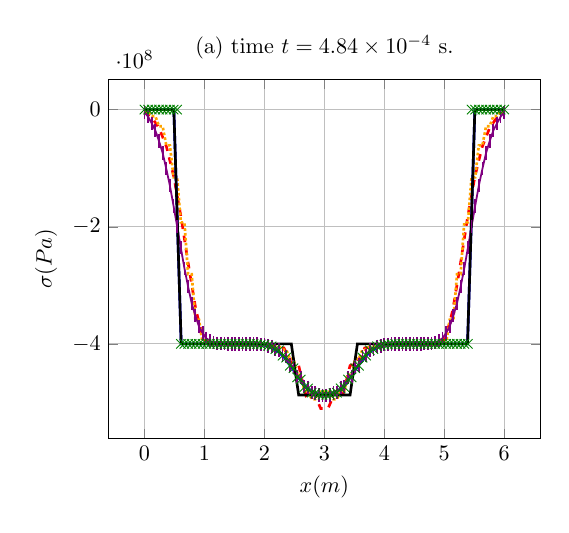
\begin{tikzpicture}[scale=0.8]
\begin{axis}[xlabel=$x (m)$,ylabel=$\sigma (Pa)$,ymajorgrids=true,xmajorgrids=true,legend pos=outer north east,title={(a) time $t = 4.84\times 10^{-4} $ s.}]
\addplot[Red,very thick,mark=none,dashed,mark size=3pt] coordinates {(0.0,-3669561.908091424) (0.12244897959183673,-13594450.379485756) (0.24489795918367346,-31624435.10565728) (0.36734693877551017,-63707048.32128755) (0.4897959183673469,-114660806.5675256) (0.6122448979591837,-184794660.6509606) (0.7346938775510203,-266179173.63903272) (0.8571428571428571,-341775310.1478163) (0.9795918367346939,-390693099.4776282) (1.1020408163265305,-400379159.02115166) (1.2244897959183674,-400770866.2752631) (1.346938775510204,-400849758.67078286) (1.4693877551020407,-400903087.2437715) (1.5918367346938775,-400974206.0457186) (1.7142857142857142,-401177729.4632526) (1.836734693877551,-401187799.71208847) (1.9591836734693877,-401722959.3911894) (2.0816326530612246,-401625095.9277148) (2.204081632653061,-405721718.460188) (2.326530612244898,-406980928.2270958) (2.4489795918367347,-432556847.70391244) (2.571428571428571,-437038541.50331527) (2.693877551020408,-488555362.3021708) (2.816326530612245,-481341619.82050365) (2.9387755102040813,-510307309.7388937) (3.061224489795918,-510307309.7388923) (3.183673469387755,-481341619.8205054) (3.306122448979592,-488555362.3021694) (3.4285714285714284,-437038541.50331557) (3.5510204081632653,-432556847.70391184) (3.673469387755102,-406980928.2270957) (3.7959183673469385,-405721718.4601879) (3.9183673469387754,-401625095.9277147) (4.040816326530612,-401722959.3911895) (4.163265306122449,-401187799.71208847) (4.285714285714286,-401177729.4632526) (4.408163265306122,-400974206.0457186) (4.530612244897959,-400903087.2437715) (4.653061224489796,-400849758.670783) (4.775510204081632,-400770866.2752632) (4.8979591836734695,-400379159.02115154) (5.020408163265306,-390693099.47762805) (5.142857142857142,-341775310.1478161) (5.26530612244898,-266179173.63903314) (5.387755102040816,-184794660.65096068) (5.5102040816326525,-114660806.56752594) (5.63265306122449,-63707048.32128816) (5.755102040816326,-31624435.10565742) (5.877551020408163,-13594450.3794861) (6.0,-3669561.9080915614) };
\addplot[Orange,very thick,mark=none,densely dotted,mark size=3pt] coordinates {(0.0,-2914267.3201301154) (0.06060606060606061,-2914267.3201301154) (0.12121212121212122,-11378318.451142035) (0.18181818181818182,-11378318.451142035) (0.24242424242424243,-28406466.993262846) (0.30303030303030304,-28406466.993262846) (0.36363636363636365,-61055835.593559496) (0.42424242424242425,-61055835.593559496) (0.48484848484848486,-115583582.76704544) (0.5454545454545454,-115583582.76704544) (0.6060606060606061,-192564241.19110337) (0.6666666666666667,-192564241.19110337) (0.7272727272727273,-281227079.2224079) (0.7878787878787878,-281227079.2224079) (0.8484848484848485,-358622783.83691025) (0.9090909090909092,-358622783.83691025) (0.9696969696969697,-399584151.64208454) (1.0303030303030303,-399584151.64208454) (1.0909090909090908,-400518950.3403047) (1.1515151515151516,-400518950.3403047) (1.2121212121212122,-400764480.1267914) (1.2727272727272727,-400764480.1267914) (1.3333333333333335,-400835508.12332404) (1.393939393939394,-400835508.12332404) (1.4545454545454546,-400891006.2882111) (1.5151515151515151,-400891006.2882111) (1.5757575757575757,-400939762.1508219) (1.6363636363636365,-400939762.1508219) (1.696969696969697,-401049302.5008664) (1.7575757575757576,-401049302.5008664) (1.8181818181818183,-401273466.6129426) (1.878787878787879,-401273466.6129426) (1.9393939393939394,-401521516.00275475) (2.0,-401521516.00275475) (2.0606060606060606,-402092208.5638283) (2.121212121212121,-402092208.5638283) (2.1818181818181817,-404027519.3843328) (2.2424242424242427,-404027519.3843328) (2.303030303030303,-409750544.23386204) (2.3636363636363638,-409750544.23386204) (2.4242424242424243,-425145499.736588) (2.484848484848485,-425145499.736588) (2.5454545454545454,-452445709.1416535) (2.606060606060606,-452445709.1416535) (2.666666666666667,-479926155.3868412) (2.7272727272727275,-479926155.3868412) (2.787878787878788,-494460484.088121) (2.8484848484848486,-494460484.088121) (2.909090909090909,-481596066.8615678) (2.9696969696969697,-481596066.8615678) (3.0303030303030303,-481596066.8615678) (3.090909090909091,-481596066.8615678) (3.1515151515151514,-494460484.088121) (3.2121212121212124,-494460484.088121) (3.272727272727273,-479926155.3868412) (3.3333333333333335,-479926155.3868412) (3.393939393939394,-452445709.1416535) (3.4545454545454546,-452445709.1416535) (3.515151515151515,-425145499.736588) (3.5757575757575757,-425145499.736588) (3.6363636363636367,-409750544.23386204) (3.6969696969696972,-409750544.23386204) (3.757575757575758,-404027519.3843328) (3.8181818181818183,-404027519.3843328) (3.878787878787879,-402092208.5638283) (3.9393939393939394,-402092208.5638283) (4.0,-401521516.0027547) (4.0606060606060606,-401521516.0027547) (4.121212121212121,-401273466.6129426) (4.181818181818182,-401273466.6129426) (4.242424242424242,-401049302.5008665) (4.303030303030303,-401049302.5008665) (4.363636363636363,-400939762.15082186) (4.424242424242425,-400939762.15082186) (4.484848484848485,-400891006.2882111) (4.545454545454546,-400891006.2882111) (4.606060606060606,-400835508.12332404) (4.666666666666667,-400835508.12332404) (4.7272727272727275,-400764480.1267914) (4.787878787878788,-400764480.1267914) (4.848484848484849,-400518950.3403046) (4.909090909090909,-400518950.3403046) (4.96969696969697,-399584151.6420844) (5.03030303030303,-399584151.6420844) (5.090909090909091,-358622783.8369101) (5.151515151515151,-358622783.8369101) (5.212121212121212,-281227079.22240764) (5.2727272727272725,-281227079.22240764) (5.333333333333334,-192564241.19110358) (5.3939393939393945,-192564241.19110358) (5.454545454545455,-115583582.76704524) (5.515151515151516,-115583582.76704524) (5.575757575757576,-61055835.59355964) (5.636363636363637,-61055835.59355964) (5.696969696969697,-28406466.99326251) (5.757575757575758,-28406466.99326251) (5.818181818181818,-11378318.451142171) (5.878787878787879,-11378318.451142171) (5.9393939393939394,-2914267.3201301834) (6.0,-2914267.3201301834) };
\addplot[Blue,very thick,mark=none,solid,mark size=3pt] coordinates {(0.0,-1.4032094709741823e-07) (0.12244897959183673,1.4032094709741797e-07) (0.24489795918367346,-5.501313561848306e-23) (0.36734693877551017,-1.4032094709741882e-07) (0.4897959183673469,-4.2096284129225576e-07) (0.6122448979591837,-400000000.0000052) (0.7346938775510203,-400000000.0003803) (0.8571428571428571,-400000000.0131417) (0.9795918367346939,-400000000.2874559) (1.1020408163265305,-400000004.46415013) (1.2244897959183674,-400000052.34678423) (1.346938775510204,-400000481.2046858) (1.4693877551020407,-400003554.03647596) (1.5918367346938775,-400021443.0967657) (1.7142857142857142,-400106894.9802318) (1.836734693877551,-400443646.6051052) (1.9591836734693877,-401540408.59283984) (2.0816326530612246,-404487333.2231472) (2.204081632653061,-410984305.87262785) (2.326530612244898,-422622254.02503896) (2.4489795918367347,-439299786.1010327) (2.571428571428571,-457971198.93456453) (2.693877551020408,-473710434.18348145) (2.816326530612245,-483108267.7934754) (2.9387755102040813,-486652315.1909913) (3.061224489795918,-486652315.1909913) (3.183673469387755,-483108267.7934754) (3.306122448979592,-473710434.18348145) (3.4285714285714284,-457971198.93456453) (3.5510204081632653,-439299786.1010328) (3.673469387755102,-422622254.025039) (3.7959183673469385,-410984305.8726279) (3.9183673469387754,-404487333.2231472) (4.040816326530612,-401540408.59283984) (4.163265306122449,-400443646.6051051) (4.285714285714286,-400106894.98023176) (4.408163265306122,-400021443.0967656) (4.530612244897959,-400003554.0364758) (4.653061224489796,-400000481.20468575) (4.775510204081632,-400000052.3467841) (4.8979591836734695,-400000004.46415013) (5.020408163265306,-400000000.2874559) (5.142857142857142,-400000000.01314175) (5.26530612244898,-400000000.0003803) (5.387755102040816,-400000000.0000052) (5.5102040816326525,1.403209470974181e-07) (5.63265306122449,-4.209628412922546e-07) (5.755102040816326,-7.335084749131074e-23) (5.877551020408163,-7.335084749131074e-23) (6.0,1.4032094709741816e-07) };
\addplot[Purple,thick,mark=|,solid,mark size=3pt] coordinates {(0.0,-4432924.706841537) (0.06060606060606061,-12207367.937325412) (0.12121212121212122,-23531843.32279323) (0.18181818181818182,-35734156.38126936) (0.24242424242424243,-53819967.0341102) (0.30303030303030304,-73960503.34391399) (0.36363636363636365,-100971777.07395627) (0.42424242424242425,-130109924.83030084) (0.48484848484848486,-164461120.69762146) (0.5454545454545454,-199783681.59143203) (0.6060606060606061,-235957589.20194656) (0.6666666666666667,-271228096.10690445) (0.7272727272727273,-302213993.4219046) (0.7878787878787878,-330771054.2743039) (0.8484848484848485,-351899554.770462) (0.9090909090909092,-370258280.79493797) (0.9696969696969697,-381361519.41978526) (1.0303030303030303,-390443246.24646133) (1.0909090909090908,-394697061.64063984) (1.1515151515151516,-397978403.46801) (1.2121212121212122,-399033797.91006035) (1.2727272727272727,-399815009.1781527) (1.3333333333333335,-399928549.7385389) (1.393939393939394,-400001024.16277933) (1.4545454545454546,-400002181.8139095) (1.5151515151515151,-400003409.2713153) (1.5757575757575757,-400013260.9517136) (1.6363636363636365,-400019327.12601054) (1.696969696969697,-400071982.9779926) (1.7575757575757576,-400098745.1685716) (1.8181818181818183,-400318321.7394188) (1.878787878787879,-400414890.0391485) (1.9393939393939394,-401165297.85083073) (2.0,-401450756.0252169) (2.0606060606060606,-403565545.76565593) (2.121212121212121,-404257062.9865757) (2.1818181818181817,-409162020.12612975) (2.2424242424242427,-410524033.8850246) (2.303030303030303,-419802201.6406596) (2.3636363636363638,-421949146.8716409) (2.4242424242424243,-436028496.5842672) (2.484848484848485,-438667957.45895886) (2.5454545454545454,-455363332.4481878) (2.606060606060606,-457791067.839726) (2.666666666666667,-472627847.3837442) (2.7272727272727275,-474182129.162814) (2.787878787878788,-483383494.6652765) (2.8484848484848486,-483980615.0668598) (2.909090909090909,-487493210.5310644) (2.9696969696969697,-487590657.9314887) (3.0303030303030303,-487590657.9314887) (3.090909090909091,-487493210.5310644) (3.1515151515151514,-483980615.0668598) (3.2121212121212124,-483383494.6652765) (3.272727272727273,-474182129.162814) (3.3333333333333335,-472627847.38374436) (3.393939393939394,-457791067.839726) (3.4545454545454546,-455363332.4481878) (3.515151515151515,-438667957.458959) (3.5757575757575757,-436028496.5842673) (3.6363636363636367,-421949146.871641) (3.6969696969696972,-419802201.6406597) (3.757575757575758,-410524033.8850248) (3.8181818181818183,-409162020.1261299) (3.878787878787879,-404257062.98657584) (3.9393939393939394,-403565545.765656) (4.0,-401450756.0252169) (4.0606060606060606,-401165297.85083085) (4.121212121212121,-400414890.0391486) (4.181818181818182,-400318321.7394188) (4.242424242424242,-400098745.1685716) (4.303030303030303,-400071982.9779927) (4.363636363636363,-400019327.12601066) (4.424242424242425,-400013260.95171374) (4.484848484848485,-400003409.2713153) (4.545454545454546,-400002181.8139095) (4.606060606060606,-400001024.16277933) (4.666666666666667,-399928549.7385392) (4.7272727272727275,-399815009.17815316) (4.787878787878788,-399033797.9100607) (4.848484848484849,-397978403.46801054) (4.909090909090909,-394697061.6406404) (4.96969696969697,-390443246.24646163) (5.03030303030303,-381361519.4197858) (5.090909090909091,-370258280.7949385) (5.151515151515151,-351899554.7704626) (5.212121212121212,-330771054.27430445) (5.2727272727272725,-302213993.42190534) (5.333333333333334,-271228096.1069048) (5.3939393939393945,-235957589.201947) (5.454545454545455,-199783681.5914322) (5.515151515151516,-164461120.6976217) (5.575757575757576,-130109924.83030085) (5.636363636363637,-100971777.07395627) (5.696969696969697,-73960503.34391414) (5.757575757575758,-53819967.034110345) (5.818181818181818,-35734156.38126946) (5.878787878787879,-23531843.322793126) (5.9393939393939394,-12207367.937325357) (6.0,-4432924.706841591) };
\addplot[Green,thin,mark=x,only marks,mark size=3pt] coordinates {(0.0,1.2652173515404603e-06) (0.06060606060606061,9.799178020182319e-07) (0.12121212121212122,-4.084567774230407e-07) (0.18181818181818182,-4.3346890516146844e-07) (0.24242424242424243,4.563473356624432e-07) (0.30303030303030304,3.855783469220664e-07) (0.36363636363636365,-5.846850939002003e-07) (0.42424242424242425,-8.185243770739822e-07) (0.48484848484848486,5.883985548618523e-07) (0.5454545454545454,8.148109161123314e-07) (0.6060606060606061,-400000000.0000001) (0.6666666666666667,-400000000.0000003) (0.7272727272727273,-400000000.00001395) (0.7878787878787878,-400000000.0000309) (0.8484848484848485,-400000000.0007001) (0.9090909090909092,-400000000.0014903) (0.9696969696969697,-400000000.0219135) (1.0303030303030303,-400000000.0446493) (1.0909090909090908,-400000000.4778095) (1.1515151515151516,-400000000.93062043) (1.2121212121212122,-400000007.7115201) (1.2727272727272727,-400000014.3371707) (1.3333333333333335,-400000095.54857785) (1.393939393939394,-400000169.3314061) (1.4545454545454546,-400000930.466908) (1.5151515151515151,-400001569.6122349) (1.5757575757575757,-400007232.7377954) (1.6363636363636365,-400011597.9099656) (1.696969696969697,-400045337.5232003) (1.7575757575757576,-400069019.1005317) (1.8181818181818183,-400230656.1994125) (1.878787878787879,-400332993.2150553) (1.9393939393939394,-400955956.96957076) (2.0,-401307731.2616477) (2.0606060606060606,-403233382.7711176) (2.121212121212121,-404189912.7567165) (2.1818181818181817,-408931765.9664936) (2.2424242424242427,-410968365.8644036) (2.303030303030303,-420167583.50623786) (2.3636363636363638,-423508767.0960166) (2.4242424242424243,-437335267.865692) (2.484848484848485,-441457068.1017972) (2.5454545454545454,-457161702.9599444) (2.606060606060606,-460844115.7211842) (2.666666666666667,-473822399.01136905) (2.7272727272727275,-476062326.4885395) (2.787878787878788,-483396938.4157252) (2.8484848484848486,-484223655.8917301) (2.909090909090909,-486749500.07510275) (2.9696969696969697,-486888696.01046515) (3.0303030303030303,-486888696.01046515) (3.090909090909091,-486749500.07510275) (3.1515151515151514,-484223655.8917301) (3.2121212121212124,-483396938.4157252) (3.272727272727273,-476062326.4885395) (3.3333333333333335,-473822399.0113689) (3.393939393939394,-460844115.721184) (3.4545454545454546,-457161702.9599444) (3.515151515151515,-441457068.1017974) (3.5757575757575757,-437335267.865692) (3.6363636363636367,-423508767.0960167) (3.6969696969696972,-420167583.506238) (3.757575757575758,-410968365.8644036) (3.8181818181818183,-408931765.9664936) (3.878787878787879,-404189912.7567166) (3.9393939393939394,-403233382.7711176) (4.0,-401307731.2616477) (4.0606060606060606,-400955956.9695708) (4.121212121212121,-400332993.2150553) (4.181818181818182,-400230656.1994125) (4.242424242424242,-400069019.1005317) (4.303030303030303,-400045337.5232003) (4.363636363636363,-400011597.9099656) (4.424242424242425,-400007232.7377954) (4.484848484848485,-400001569.6122349) (4.545454545454546,-400000930.466908) (4.606060606060606,-400000169.3314062) (4.666666666666667,-400000095.5485779) (4.7272727272727275,-400000014.3371707) (4.787878787878788,-400000007.7115201) (4.848484848484849,-400000000.93062043) (4.909090909090909,-400000000.4778095) (4.96969696969697,-400000000.04464936) (5.03030303030303,-400000000.02191347) (5.090909090909091,-400000000.0014904) (5.151515151515151,-400000000.00070024) (5.212121212121212,-400000000.0000309) (5.2727272727272725,-400000000.0000138) (5.333333333333334,-400000000.00000036) (5.3939393939393945,-400000000.0000002) (5.454545454545455,5.066066144912661e-07) (5.515151515151516,6.159609622880803e-07) (5.575757575757576,-1.4374680478850218e-07) (5.636363636363637,-4.1753698360117076e-07) (5.696969696969697,-4.929735310217885e-07) (5.757575757575758,-6.295940457575577e-07) (5.818181818181818,1.5312531108404206e-06) (5.878787878787879,1.5558077253027814e-06) (5.9393939393939394,-3.6714372754933455e-07) (6.0,-1.9414006084033805e-07) };
\addplot[black,very thick,mark=pentagone*,solid,mark size=3pt] coordinates {(0.0,-0.0) (0.12244897959183673,-0.0) (0.24489795918367346,-0.0) (0.36734693877551017,-0.0) (0.4897959183673469,-0.0) (0.6122448979591837,-400000000.0) (0.7346938775510203,-400000000.0) (0.8571428571428571,-400000000.0) (0.9795918367346939,-400000000.0) (1.1020408163265305,-400000000.0) (1.2244897959183674,-400000000.0) (1.346938775510204,-400000000.0) (1.4693877551020407,-400000000.0) (1.5918367346938775,-400000000.0) (1.7142857142857142,-400000000.0) (1.836734693877551,-400000000.0) (1.9591836734693877,-400000000.0) (2.0816326530612246,-400000000.0) (2.204081632653061,-400000000.0) (2.326530612244898,-400000000.0) (2.4489795918367347,-400000000.0) (2.571428571428571,-487287156.09439695) (2.693877551020408,-487287156.09439695) (2.816326530612245,-487287156.09439695) (2.9387755102040813,-487287156.09439695) (3.061224489795918,-487287156.09439695) (3.183673469387755,-487287156.09439695) (3.306122448979592,-487287156.09439695) (3.4285714285714284,-487287156.09439695) (3.5510204081632653,-400000000.0) (3.673469387755102,-400000000.0) (3.7959183673469385,-400000000.0) (3.9183673469387754,-400000000.0) (4.040816326530612,-400000000.0) (4.163265306122449,-400000000.0) (4.285714285714286,-400000000.0) (4.408163265306122,-400000000.0) (4.530612244897959,-400000000.0) (4.653061224489796,-400000000.0) (4.775510204081632,-400000000.0) (4.8979591836734695,-400000000.0) (5.020408163265306,-400000000.0) (5.142857142857142,-400000000.0) (5.26530612244898,-400000000.0) (5.387755102040816,-400000000.0) (5.5102040816326525,-0.0) (5.63265306122449,-0.0) (5.755102040816326,-0.0) (5.877551020408163,-0.0) (6.0,-0.0) };
%\legend{usl 1ppc,usl 2ppc,dgmpm 1ppc,dgmpm 2ppc,dgmpm 2ppc (RK2),exact}
\end{axis}
\end{tikzpicture}
%%% Local Variables:
%%% mode: latex
%%% TeX-master: "../../mainManuscript"
%%% End:
}
%   % {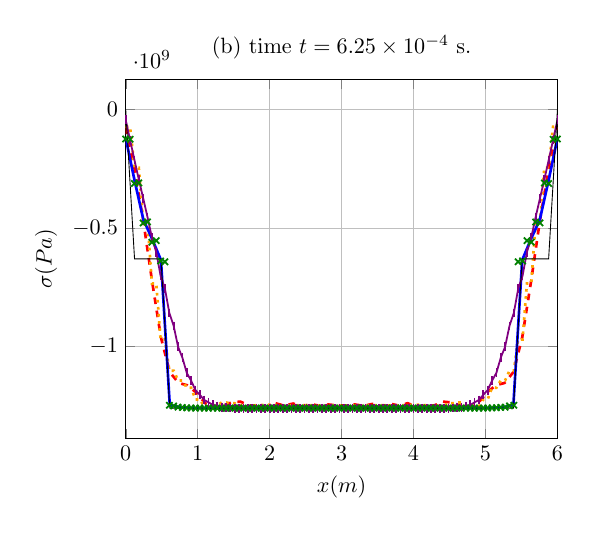
\begin{tikzpicture}[scale=0.8]
\begin{axis}[xlabel=$x (m)$,ylabel=$\sigma (Pa)$,ymajorgrids=true,xmajorgrids=true,legend pos=outer north east,title={(b) time $t = 6.25\times 10^{-4} $ s.},xmin=0.,xmax=6.]
\addplot[Red,very thick,mark=none,dashed] coordinates {(0.0,-74686690.65430246) (0.12244897959183673,-248860978.1693335) (0.24489795918367346,-471505677.3136862) (0.36734693877551017,-727347550.4714894) (0.4897959183673469,-963308331.6520433) (0.6122448979591837,-1108824904.6085515) (0.7346938775510203,-1154837713.915547) (0.8571428571428571,-1164658358.6882505) (0.9795918367346939,-1195327833.6731591) (1.1020408163265305,-1239722495.17177) (1.2244897959183674,-1262625036.5763078) (1.346938775510204,-1250850727.3360605) (1.4693877551020407,-1237335621.1098552) (1.5918367346938775,-1233570784.670482) (1.7142857142857142,-1250022356.590519) (1.836734693877551,-1250064510.2383804) (1.9591836734693877,-1255304260.9119728) (2.0816326530612246,-1240464014.9742188) (2.204081632653061,-1250749408.0219655) (2.326530612244898,-1241771881.0316234) (2.4489795918367347,-1254655253.5739675) (2.571428571428571,-1243386642.1602688) (2.693877551020408,-1251564997.8232079) (2.816326530612245,-1245650942.428049) (2.9387755102040813,-1249901934.3884947) (3.061224489795918,-1249901934.3884926) (3.183673469387755,-1245650942.4280505) (3.306122448979592,-1251564997.8232062) (3.4285714285714284,-1243386642.160271) (3.5510204081632653,-1254655253.5739667) (3.673469387755102,-1241771881.0316243) (3.7959183673469385,-1250749408.0219643) (3.9183673469387754,-1240464014.9742193) (4.040816326530612,-1255304260.911973) (4.163265306122449,-1250064510.238382) (4.285714285714286,-1250022356.59052) (4.408163265306122,-1233570784.670483) (4.530612244897959,-1237335621.1098552) (4.653061224489796,-1250850727.3360612) (4.775510204081632,-1262625036.5763083) (4.8979591836734695,-1239722495.1717708) (5.020408163265306,-1195327833.6731594) (5.142857142857142,-1164658358.688251) (5.26530612244898,-1154837713.915547) (5.387755102040816,-1108824904.6085508) (5.5102040816326525,-963308331.652042) (5.63265306122449,-727347550.4714878) (5.755102040816326,-471505677.3136848) (5.877551020408163,-248860978.16933236) (6.0,-74686690.65430167) };
\addplot[Orange,very thick,mark=none,dotted] coordinates {(0.0,-72186593.07108305) (0.06060606060606061,-72186593.07108305) (0.12121212121212122,-245686493.40496877) (0.18181818181818182,-245686493.40496877) (0.24242424242424243,-474670673.0513873) (0.30303030303030304,-474670673.0513873) (0.36363636363636365,-734906817.2671752) (0.42424242424242425,-734906817.2671752) (0.48484848484848486,-970962001.9023491) (0.5454545454545454,-970962001.9023491) (0.6060606060606061,-1103271474.8574238) (0.6666666666666667,-1103271474.8574238) (0.7272727272727273,-1144170322.1258416) (0.7878787878787878,-1144170322.1258416) (0.8484848484848485,-1175098111.1407657) (0.9090909090909092,-1175098111.1407657) (0.9696969696969697,-1224410658.5301867) (1.0303030303030303,-1224410658.5301867) (1.0909090909090908,-1254385387.017002) (1.1515151515151516,-1254385387.017002) (1.2121212121212122,-1249105579.9476206) (1.2727272727272727,-1249105579.9476206) (1.3333333333333335,-1237157219.1940255) (1.393939393939394,-1237157219.1940255) (1.4545454545454546,-1240480450.514414) (1.5151515151515151,-1240480450.514414) (1.5757575757575757,-1250188640.1270242) (1.6363636363636365,-1250188640.1270242) (1.696969696969697,-1252250954.763) (1.7575757575757576,-1252250954.763) (1.8181818181818183,-1248402726.9188023) (1.878787878787879,-1248402726.9188023) (1.9393939393939394,-1246829218.0208151) (2.0,-1246829218.0208151) (2.0606060606060606,-1248579916.6035461) (2.121212121212121,-1248579916.6035461) (2.1818181818181817,-1249829973.3539176) (2.2424242424242427,-1249829973.3539176) (2.303030303030303,-1249407075.968172) (2.3636363636363638,-1249407075.968172) (2.4242424242424243,-1248930440.9460857) (2.484848484848485,-1248930440.9460857) (2.5454545454545454,-1249182413.9939532) (2.606060606060606,-1249182413.9939532) (2.666666666666667,-1249584324.22758) (2.7272727272727275,-1249584324.22758) (2.787878787878788,-1249734146.6328998) (2.8484848484848486,-1249734146.6328998) (2.909090909090909,-1249747490.5668778) (2.9696969696969697,-1249747490.5668778) (3.0303030303030303,-1249747490.5668783) (3.090909090909091,-1249747490.5668783) (3.1515151515151514,-1249734146.6329007) (3.2121212121212124,-1249734146.6329007) (3.272727272727273,-1249584324.2275805) (3.3333333333333335,-1249584324.2275805) (3.393939393939394,-1249182413.993953) (3.4545454545454546,-1249182413.993953) (3.515151515151515,-1248930440.946085) (3.5757575757575757,-1248930440.946085) (3.6363636363636367,-1249407075.9681716) (3.6969696969696972,-1249407075.9681716) (3.757575757575758,-1249829973.3539178) (3.8181818181818183,-1249829973.3539178) (3.878787878787879,-1248579916.6035466) (3.9393939393939394,-1248579916.6035466) (4.0,-1246829218.0208151) (4.0606060606060606,-1246829218.0208151) (4.121212121212121,-1248402726.9188023) (4.181818181818182,-1248402726.9188023) (4.242424242424242,-1252250954.7630002) (4.303030303030303,-1252250954.7630002) (4.363636363636363,-1250188640.1270244) (4.424242424242425,-1250188640.1270244) (4.484848484848485,-1240480450.5144138) (4.545454545454546,-1240480450.5144138) (4.606060606060606,-1237157219.194025) (4.666666666666667,-1237157219.194025) (4.7272727272727275,-1249105579.9476204) (4.787878787878788,-1249105579.9476204) (4.848484848484849,-1254385387.0170026) (4.909090909090909,-1254385387.0170026) (4.96969696969697,-1224410658.5301871) (5.03030303030303,-1224410658.5301871) (5.090909090909091,-1175098111.140766) (5.151515151515151,-1175098111.140766) (5.212121212121212,-1144170322.125842) (5.2727272727272725,-1144170322.125842) (5.333333333333334,-1103271474.8574243) (5.3939393939393945,-1103271474.8574243) (5.454545454545455,-970962001.902349) (5.515151515151516,-970962001.902349) (5.575757575757576,-734906817.2671752) (5.636363636363637,-734906817.2671752) (5.696969696969697,-474670673.05138755) (5.757575757575758,-474670673.05138755) (5.818181818181818,-245686493.40496898) (5.878787878787879,-245686493.40496898) (5.9393939393939394,-72186593.0710832) (6.0,-72186593.0710832) };
\addplot[Blue,very thick,mark=none,solid] coordinates {(0.0,-120597397.19248778) (0.12244897959183673,-298539345.15508544) (0.24489795918367346,-464504460.170754) (0.36734693877551017,-546627376.3559334) (0.4897959183673469,-635546108.2543886) (0.6122448979591837,-1247334335.3333962) (0.7346938775510203,-1255980074.5990539) (0.8571428571428571,-1259371705.5275755) (0.9795918367346939,-1260535220.1287405) (1.1020408163265305,-1260885267.5005968) (1.2244897959183674,-1260977777.705495) (1.346938775510204,-1260999265.6570995) (1.4693877551020407,-1261003650.0375175) (1.5918367346938775,-1261004434.5740557) (1.7142857142857142,-1261004557.3391547) (1.836734693877551,-1261004574.0682204) (1.9591836734693877,-1261004576.0419452) (2.0816326530612246,-1261004576.241996) (2.204081632653061,-1261004576.2592359) (2.326530612244898,-1261004576.260481) (2.4489795918367347,-1261004576.260556) (2.571428571428571,-1261004576.2605588) (2.693877551020408,-1261004576.260559) (2.816326530612245,-1261004576.2605588) (2.9387755102040813,-1261004576.260559) (3.061224489795918,-1261004576.2605584) (3.183673469387755,-1261004576.2605586) (3.306122448979592,-1261004576.2605588) (3.4285714285714284,-1261004576.2605581) (3.5510204081632653,-1261004576.2605555) (3.673469387755102,-1261004576.260481) (3.7959183673469385,-1261004576.2592354) (3.9183673469387754,-1261004576.2419953) (4.040816326530612,-1261004576.0419443) (4.163265306122449,-1261004574.06822) (4.285714285714286,-1261004557.3391542) (4.408163265306122,-1261004434.5740552) (4.530612244897959,-1261003650.037517) (4.653061224489796,-1260999265.6570988) (4.775510204081632,-1260977777.7054946) (4.8979591836734695,-1260885267.500596) (5.020408163265306,-1260535220.1287398) (5.142857142857142,-1259371705.5275738) (5.26530612244898,-1255980074.5990536) (5.387755102040816,-1247334335.3333952) (5.5102040816326525,-635546108.2543867) (5.63265306122449,-546627376.3559326) (5.755102040816326,-464504460.1707534) (5.877551020408163,-298539345.15508515) (6.0,-120597397.19248791) };
\addplot[Purple,thick,mark=|,solid] coordinates {(0.0,-43439158.01953824) (0.06060606060606061,-128494718.82956168) (0.12121212121212122,-212712806.4484778) (0.18181818181818182,-294968746.093467) (0.24242424242424243,-374066686.2634123) (0.30303030303030304,-454380990.25937665) (0.36363636363636365,-540156903.2805651) (0.42424242424242425,-602480956.5032418) (0.48484848484848486,-702661585.1512607) (0.5454545454545454,-756997379.9274446) (0.6060606060606061,-859011324.2404706) (0.6666666666666667,-914140387.8341031) (0.7272727272727273,-1001733202.5250769) (0.7878787878787878,-1048303078.4017226) (0.8484848484848485,-1112416155.8061078) (0.9090909090909092,-1145155832.8175488) (0.9696969696969697,-1185261988.985457) (1.0303030303030303,-1204786235.0815058) (1.0909090909090908,-1226655831.3690634) (1.1515151515151516,-1236845694.8683596) (1.2121212121212122,-1247415339.0967982) (1.2727272727272727,-1252155381.0243487) (1.3333333333333335,-1256710201.5466359) (1.393939393939394,-1258689335.4211235) (1.4545454545454546,-1260456486.190056) (1.5151515151515151,-1261197436.235882) (1.5757575757575757,-1261810365.4044876) (1.6363636363636365,-1262048555.9214687) (1.696969696969697,-1262232771.7377496) (1.7575757575757576,-1262267932.0178628) (1.8181818181818183,-1262317140.869429) (1.878787878787879,-1262273539.5537865) (1.9393939393939394,-1262278489.6867273) (2.0,-1262229915.5005774) (2.0606060606060606,-1262220408.763863) (2.121212121212121,-1262174209.4696336) (2.1818181818181817,-1262179981.2050242) (2.2424242424242427,-1262122756.5305994) (2.303030303030303,-1262166768.744628) (2.3636363636363638,-1262087669.6055806) (2.4242424242424243,-1262155242.0676785) (2.484848484848485,-1262097413.4000623) (2.5454545454545454,-1262171888.997602) (2.606060606060606,-1262117114.7579942) (2.666666666666667,-1262226451.4058053) (2.7272727272727275,-1262121200.847136) (2.787878787878788,-1262339443.020975) (2.8484848484848486,-1262066956.6541011) (2.909090909090909,-1262521430.1991065) (2.9696969696969697,-1261921359.640449) (3.0303030303030303,-1261921359.6404493) (3.090909090909091,-1262521430.1991067) (3.1515151515151514,-1262066956.6541014) (3.2121212121212124,-1262339443.0209754) (3.272727272727273,-1262121200.8471358) (3.3333333333333335,-1262226451.405806) (3.393939393939394,-1262117114.7579951) (3.4545454545454546,-1262171888.9976025) (3.515151515151515,-1262097413.4000628) (3.5757575757575757,-1262155242.0676794) (3.6363636363636367,-1262087669.6055813) (3.6969696969696972,-1262166768.744628) (3.757575757575758,-1262122756.5305994) (3.8181818181818183,-1262179981.2050242) (3.878787878787879,-1262174209.4696333) (3.9393939393939394,-1262220408.7638628) (4.0,-1262229915.5005774) (4.0606060606060606,-1262278489.6867273) (4.121212121212121,-1262273539.5537865) (4.181818181818182,-1262317140.8694305) (4.242424242424242,-1262267932.0178633) (4.303030303030303,-1262232771.7377505) (4.363636363636363,-1262048555.9214697) (4.424242424242425,-1261810365.4044883) (4.484848484848485,-1261197436.2358823) (4.545454545454546,-1260456486.1900568) (4.606060606060606,-1258689335.4211237) (4.666666666666667,-1256710201.5466368) (4.7272727272727275,-1252155381.0243497) (4.787878787878788,-1247415339.096799) (4.848484848484849,-1236845694.8683605) (4.909090909090909,-1226655831.3690639) (4.96969696969697,-1204786235.0815067) (5.03030303030303,-1185261988.9854574) (5.090909090909091,-1145155832.8175497) (5.151515151515151,-1112416155.8061085) (5.212121212121212,-1048303078.4017233) (5.2727272727272725,-1001733202.5250776) (5.333333333333334,-914140387.834104) (5.3939393939393945,-859011324.2404717) (5.454545454545455,-756997379.9274455) (5.515151515151516,-702661585.1512614) (5.575757575757576,-602480956.5032421) (5.636363636363637,-540156903.2805656) (5.696969696969697,-454380990.25937706) (5.757575757575758,-374066686.26341283) (5.818181818181818,-294968746.09346735) (5.878787878787879,-212712806.44847828) (5.9393939393939394,-128494718.82956178) (6.0,-43439158.019538306) };
\addplot[Green,thick,mark=x,only marks] coordinates {(0.0,-124149916.18460932) (0.06060606060606061,-125384025.95198976) (0.12121212121212122,-312191395.454492) (0.18181818181818182,-309823612.32028496) (0.24242424242424243,-478839586.50914454) (0.30303030303030304,-474422726.8389135) (0.36363636363636365,-560023095.785606) (0.42424242424242425,-553441168.2048206) (0.48484848484848486,-639348195.1618631) (0.5454545454545454,-642840843.3429394) (0.6060606060606061,-1249244226.3218632) (0.6666666666666667,-1251996686.3855102) (0.7272727272727273,-1257129205.37515) (0.7878787878787878,-1258189385.686948) (0.8484848484848485,-1259909142.5036347) (0.9090909090909092,-1260253063.700632) (0.9696969696969697,-1260739786.195639) (1.0303030303030303,-1260833818.3494694) (1.0909090909090908,-1260950011.0851812) (1.1515151515151516,-1260971641.1801379) (1.2121212121212122,-1260995018.2511435) (1.2727272727272727,-1260999205.0818741) (1.3333333333333335,-1261003073.8839324) (1.393939393939394,-1261003729.7383952) (1.4545454545454546,-1261004222.6859503) (1.5151515151515151,-1261004299.406877) (1.5757575757575757,-1261004499.1892421) (1.6363636363636365,-1261004544.8157115) (1.696969696969697,-1261004335.4465394) (1.7575757575757576,-1261004315.5457916) (1.8181818181818183,-1261004554.3249235) (1.878787878787879,-1261004539.201182) (1.9393939393939394,-1261004509.2896533) (2.0,-1261004479.0183125) (2.0606060606060606,-1261004581.0248919) (2.121212121212121,-1261004530.8669846) (2.1818181818181817,-1261004594.5349371) (2.2424242424242427,-1261004535.9740446) (2.303030303030303,-1261004688.980403) (2.3636363636363638,-1261004531.5634973) (2.4242424242424243,-1261004753.5964737) (2.484848484848485,-1261004491.241939) (2.5454545454545454,-1261004855.8046663) (2.606060606060606,-1261004170.2011797) (2.666666666666667,-1261005415.5085306) (2.7272727272727275,-1261003664.942618) (2.787878787878788,-1261005905.0268464) (2.8484848484848486,-1261003146.0581243) (2.909090909090909,-1261018444.8195553) (2.9696969696969697,-1260990588.6825547) (3.0303030303030303,-1260990588.6825557) (3.090909090909091,-1261018444.8195562) (3.1515151515151514,-1261003146.0581238) (3.2121212121212124,-1261005905.0268452) (3.272727272727273,-1261003664.9426184) (3.3333333333333335,-1261005415.5085318) (3.393939393939394,-1261004170.2011807) (3.4545454545454546,-1261004855.804668) (3.515151515151515,-1261004491.241938) (3.5757575757575757,-1261004753.5964735) (3.6363636363636367,-1261004531.563497) (3.6969696969696972,-1261004688.9804025) (3.757575757575758,-1261004535.9740455) (3.8181818181818183,-1261004594.5349386) (3.878787878787879,-1261004530.8669853) (3.9393939393939394,-1261004581.0248923) (4.0,-1261004479.0183132) (4.0606060606060606,-1261004509.2896538) (4.121212121212121,-1261004539.201182) (4.181818181818182,-1261004554.3249235) (4.242424242424242,-1261004315.5457911) (4.303030303030303,-1261004335.4465387) (4.363636363636363,-1261004544.815712) (4.424242424242425,-1261004499.1892428) (4.484848484848485,-1261004299.4068773) (4.545454545454546,-1261004222.6859503) (4.606060606060606,-1261003729.7383952) (4.666666666666667,-1261003073.8839328) (4.7272727272727275,-1260999205.0818748) (4.787878787878788,-1260995018.2511437) (4.848484848484849,-1260971641.1801379) (4.909090909090909,-1260950011.0851815) (4.96969696969697,-1260833818.3494704) (5.03030303030303,-1260739786.1956398) (5.090909090909091,-1260253063.7006326) (5.151515151515151,-1259909142.5036354) (5.212121212121212,-1258189385.6869476) (5.2727272727272725,-1257129205.3751497) (5.333333333333334,-1251996686.3855097) (5.3939393939393945,-1249244226.3218625) (5.454545454545455,-642840843.3429406) (5.515151515151516,-639348195.1618624) (5.575757575757576,-553441168.2048205) (5.636363636363637,-560023095.7856064) (5.696969696969697,-474422726.8389133) (5.757575757575758,-478839586.50914484) (5.818181818181818,-309823612.320285) (5.878787878787879,-312191395.4544924) (5.9393939393939394,-125384025.95198983) (6.0,-124149916.18460946) };
\addplot[black,thin,mark=none,solid] coordinates {(0.0,-0.0) (0.12244897959183673,-630502288.1302795) (0.24489795918367346,-630502288.1302795) (0.36734693877551017,-630502288.1302795) (0.4897959183673469,-630502288.1302795) (0.6122448979591837,-1261004576.260559) (0.7346938775510203,-1261004576.260559) (0.8571428571428571,-1261004576.260559) (0.9795918367346939,-1261004576.260559) (1.1020408163265305,-1261004576.260559) (1.2244897959183674,-1261004576.260559) (1.346938775510204,-1261004576.260559) (1.4693877551020407,-1261004576.260559) (1.5918367346938775,-1261004576.260559) (1.7142857142857142,-1261004576.260559) (1.836734693877551,-1261004576.260559) (1.9591836734693877,-1261004576.260559) (2.0816326530612246,-1261004576.260559) (2.204081632653061,-1261004576.260559) (2.326530612244898,-1261004576.260559) (2.4489795918367347,-1261004576.260559) (2.571428571428571,-1261004576.260559) (2.693877551020408,-1261004576.260559) (2.816326530612245,-1261004576.260559) (2.9387755102040813,-1261004576.260559) (3.061224489795918,-1261004576.260559) (3.183673469387755,-1261004576.260559) (3.306122448979592,-1261004576.260559) (3.4285714285714284,-1261004576.260559) (3.5510204081632653,-1261004576.260559) (3.673469387755102,-1261004576.260559) (3.7959183673469385,-1261004576.260559) (3.9183673469387754,-1261004576.260559) (4.040816326530612,-1261004576.260559) (4.163265306122449,-1261004576.260559) (4.285714285714286,-1261004576.260559) (4.408163265306122,-1261004576.260559) (4.530612244897959,-1261004576.260559) (4.653061224489796,-1261004576.260559) (4.775510204081632,-1261004576.260559) (4.8979591836734695,-1261004576.260559) (5.020408163265306,-1261004576.260559) (5.142857142857142,-1261004576.260559) (5.26530612244898,-1261004576.260559) (5.387755102040816,-1261004576.260559) (5.5102040816326525,-630502288.1302795) (5.63265306122449,-630502288.1302795) (5.755102040816326,-630502288.1302795) (5.877551020408163,-630502288.1302795) (6.0,-0.0) };
%\legend{usl 1ppc,usl 2ppc,dgmpm 1ppc,dgmpm 2ppc,dgmpm 2ppc (RK2),exact}
\end{axis}
\end{tikzpicture}
%%% Local Variables:
%%% mode: latex
%%% TeX-master: "../../mainManuscript"
%%% End:
}
%   {\begin{tikzpicture}[scale=.9]
\begin{groupplot}[group style={group size=3 by 2,
ylabels at=edge left, yticklabels at=edge left,horizontal sep=2.ex,
vertical sep=4ex,xticklabels at=edge bottom,xlabels at=edge bottom},
ymajorgrids=true,xmajorgrids=true,enlargelimits=0,xmin=0.,xmax=6.,xlabel=$x (m)$,
axis on top,scale only axis,width=0.32\linewidth
]
\nextgroupplot[title={(a) $t = 4.17\times 10^{-4} $ s.},ylabel=$\sigma (Pa)$,]
\addplot[Blue,solid,mark=none,very thick,mark size=2pt] coordinates{(0.0,-3.25611587112e-07) (0.122448979592,-6.54162606233e-22) (0.244897959184,0.0) (0.367346938776,3.25611587112e-07) (0.489795918367,-4.88417380668e-07) (0.612244897959,-706703995.006) (0.734693877551,-739923853.313) (0.857142857143,-818114621.328) (0.979591836735,-934350667.086) (1.10204081633,-1056745717.41) (1.22448979592,-1153785079.18) (1.34693877551,-1213891661.99) (1.4693877551,-1243675875.17) (1.59183673469,-1255667377.46) (1.71428571429,-1259628756.78) (1.83673469388,-1260708382.47) (1.95918367347,-1260951555.07) (2.08163265306,-1260996741.7) (2.20408163265,-1261003631.25) (2.32653061224,-1261004484.73) (2.44897959184,-1261004569.31) (2.57142857143,-1261004575.86) (2.69387755102,-1261004576.24) (2.81632653061,-1261004576.26) (2.9387755102,-1261004576.26) (3.0612244898,-1261004576.26) (3.18367346939,-1261004576.26) (3.30612244898,-1261004576.24) (3.42857142857,-1261004575.86) (3.55102040816,-1261004569.31) (3.67346938776,-1261004484.73) (3.79591836735,-1261003631.25) (3.91836734694,-1260996741.7) (4.04081632653,-1260951555.07) (4.16326530612,-1260708382.47) (4.28571428571,-1259628756.78) (4.40816326531,-1255667377.46) (4.5306122449,-1243675875.17) (4.65306122449,-1213891661.99) (4.77551020408,-1153785079.18) (4.89795918367,-1056745717.41) (5.02040816327,-934350667.086) (5.14285714286,-818114621.328) (5.26530612245,-739923853.313) (5.38775510204,-706703995.006) (5.51020408163,-4.88417380668e-07) (5.63265306122,0.0) (5.75510204082,-4.88417380668e-07) (5.87755102041,0.0) (6.0,-4.88417380668e-07) };
\addplot[Purple,only marks,mark=+,thin,mark size=2pt] coordinates{(0.0,-6327912.39976) (0.0606060606061,-17393855.4498) (0.121212121212,-34791452.0156) (0.181818181818,-54271429.8986) (0.242424242424,-85476186.7634) (0.30303030303,-121344975.529) (0.363636363636,-172772413.109) (0.424242424242,-229646809.33) (0.484848484848,-300604808.871) (0.545454545455,-374985968.406) (0.606060606061,-454379573.056) (0.666666666667,-532582620.671) (0.727272727273,-601889718.545) (0.787878787879,-665111214.747) (0.848484848485,-710389190.246) (0.909090909091,-740809726.393) (0.969696969697,-783840999.734) (1.0303030303,-822574838.477) (1.09090909091,-881869005.613) (1.15151515152,-928117392.832) (1.21212121212,-992030440.922) (1.27272727273,-1037630664.81) (1.33333333333,-1094332999.9) (1.39393939394,-1131243116.44) (1.45454545455,-1172779891.01) (1.51515151515,-1197412378.63) (1.57575757576,-1222494297.05) (1.63636363636,-1235925009.98) (1.69696969697,-1248261695.93) (1.75757575758,-1254152813.68) (1.81818181818,-1258986167.93) (1.87878787879,-1260986849.61) (1.93939393939,-1262401857.25) (2.0,-1262863321.6) (2.06060606061,-1263097274.85) (2.12121212121,-1263105090.64) (2.18181818182,-1263091292.13) (2.24242424242,-1263006777.33) (2.30303030303,-1263028365.67) (2.36363636364,-1262931396.23) (2.42424242424,-1262985011.95) (2.48484848485,-1262917562.75) (2.54545454545,-1262983412.75) (2.60606060606,-1262924149.66) (2.66666666667,-1263029713.54) (2.72727272727,-1262927168.66) (2.78787878788,-1263147911.39) (2.84848484848,-1262880892.07) (2.90909090909,-1263338476.16) (2.9696969697,-1262740516.98) (3.0303030303,-1262740516.98) (3.09090909091,-1263338476.16) (3.15151515152,-1262880892.07) (3.21212121212,-1263147911.39) (3.27272727273,-1262927168.66) (3.33333333333,-1263029713.54) (3.39393939394,-1262924149.66) (3.45454545455,-1262983412.75) (3.51515151515,-1262917562.75) (3.57575757576,-1262985011.95) (3.63636363636,-1262931396.23) (3.69696969697,-1263028365.67) (3.75757575758,-1263006777.33) (3.81818181818,-1263091292.13) (3.87878787879,-1263105090.64) (3.93939393939,-1263097274.85) (4.0,-1262863321.6) (4.06060606061,-1262401857.25) (4.12121212121,-1260986849.61) (4.18181818182,-1258986167.93) (4.24242424242,-1254152813.68) (4.30303030303,-1248261695.93) (4.36363636364,-1235925009.98) (4.42424242424,-1222494297.05) (4.48484848485,-1197412378.63) (4.54545454545,-1172779891.01) (4.60606060606,-1131243116.44) (4.66666666667,-1094332999.9) (4.72727272727,-1037630664.81) (4.78787878788,-992030440.922) (4.84848484848,-928117392.832) (4.90909090909,-881869005.613) (4.9696969697,-822574838.477) (5.0303030303,-783840999.734) (5.09090909091,-740809726.393) (5.15151515152,-710389190.246) (5.21212121212,-665111214.747) (5.27272727273,-601889718.545) (5.33333333333,-532582620.671) (5.39393939394,-454379573.056) (5.45454545455,-374985968.406) (5.51515151515,-300604808.871) (5.57575757576,-229646809.33) (5.63636363636,-172772413.109) (5.69696969697,-121344975.529) (5.75757575758,-85476186.7634) (5.81818181818,-54271429.8986) (5.87878787879,-34791452.0156) (5.93939393939,-17393855.4498) (6.0,-6327912.39976) };
\addplot[Duck,only marks,mark=x,thick,mark size=2pt] coordinates{(0.0,-9.93898524111e-07) (0.0606060606061,-1.28538258567e-06) (0.121212121212,8.20148892499e-07) (0.181818181818,4.82297455949e-07) (0.242424242424,-9.83648482392e-07) (0.30303030303,-1.29563262739e-06) (0.363636363636,1.9586488831e-06) (0.424242424242,2.59991333647e-06) (0.484848484848,-1.47908827276e-06) (0.545454545455,-1.45141601125e-06) (0.606060606061,-704729842.246) (0.666666666667,-706002047.131) (0.727272727273,-731613409.083) (0.787878787879,-738307360.325) (0.848484848485,-802443845.411) (0.909090909091,-818702029.0) (0.969696969697,-917273418.408) (1.0303030303,-941457325.325) (1.09090909091,-1045498983.94) (1.15151515152,-1070147015.02) (1.21212121212,-1150104083.78) (1.27272727273,-1168347225.69) (1.33333333333,-1214623647.02) (1.39393939394,-1224762462.12) (1.45454545455,-1245337865.77) (1.51515151515,-1249651955.8) (1.57575757576,-1256756187.73) (1.63636363636,-1258176137.8) (1.69696969697,-1260087550.93) (1.75757575758,-1260449997.18) (1.81818181818,-1260849081.88) (1.87878787879,-1260920429.98) (1.93939393939,-1260984677.09) (2.0,-1260995458.22) (2.06060606061,-1261002466.88) (2.12121212121,-1261003454.06) (2.18181818182,-1261004228.04) (2.24242424242,-1261004332.33) (2.30303030303,-1261004658.42) (2.36363636364,-1261004353.51) (2.42424242424,-1261005248.86) (2.48484848485,-1261004976.04) (2.54545454545,-1261004543.31) (2.60606060606,-1261003848.69) (2.66666666667,-1261005173.64) (2.72727272727,-1261003422.42) (2.78787878788,-1261005964.75) (2.84848484848,-1261003205.95) (2.90909090909,-1261018212.46) (2.9696969697,-1260990356.29) (3.0303030303,-1260990356.29) (3.09090909091,-1261018212.46) (3.15151515152,-1261003205.95) (3.21212121212,-1261005964.75) (3.27272727273,-1261003422.42) (3.33333333333,-1261005173.64) (3.39393939394,-1261003848.69) (3.45454545455,-1261004543.31) (3.51515151515,-1261004976.04) (3.57575757576,-1261005248.86) (3.63636363636,-1261004353.51) (3.69696969697,-1261004658.42) (3.75757575758,-1261004332.33) (3.81818181818,-1261004228.04) (3.87878787879,-1261003454.06) (3.93939393939,-1261002466.88) (4.0,-1260995458.22) (4.06060606061,-1260984677.09) (4.12121212121,-1260920429.98) (4.18181818182,-1260849081.88) (4.24242424242,-1260449997.18) (4.30303030303,-1260087550.93) (4.36363636364,-1258176137.8) (4.42424242424,-1256756187.73) (4.48484848485,-1249651955.8) (4.54545454545,-1245337865.77) (4.60606060606,-1224762462.12) (4.66666666667,-1214623647.02) (4.72727272727,-1168347225.69) (4.78787878788,-1150104083.78) (4.84848484848,-1070147015.02) (4.90909090909,-1045498983.94) (4.9696969697,-941457325.325) (5.0303030303,-917273418.408) (5.09090909091,-818702029.0) (5.15151515152,-802443845.411) (5.21212121212,-738307360.325) (5.27272727273,-731613409.083) (5.33333333333,-706002047.131) (5.39393939394,-704729842.246) (5.45454545455,-9.05250759754e-07) (5.51515151515,-7.22807175807e-07) (5.57575757576,8.56721652335e-07) (5.63636363636,7.71336283226e-07) (5.69696969697,-5.84795808728e-07) (5.75757575758,-7.17650539721e-07) (5.81818181818,1.14987423532e-06) (5.87878787879,1.45501846157e-06) (5.93939393939,-2.54796481511e-06) (6.0,-2.33620899157e-06) };
\addplot[black,solid,mark=none,thin,mark size=2pt] coordinates{(0.0,-0.0) (0.122448979592,-0.0) (0.244897959184,-0.0) (0.367346938776,-0.0) (0.489795918367,-0.0) (0.612244897959,-700000000.0) (0.734693877551,-700000000.0) (0.857142857143,-700000000.0) (0.979591836735,-700000000.0) (1.10204081633,-1261004576.26) (1.22448979592,-1261004576.26) (1.34693877551,-1261004576.26) (1.4693877551,-1261004576.26) (1.59183673469,-1261004576.26) (1.71428571429,-1261004576.26) (1.83673469388,-1261004576.26) (1.95918367347,-1261004576.26) (2.08163265306,-1261004576.26) (2.20408163265,-1261004576.26) (2.32653061224,-1261004576.26) (2.44897959184,-1261004576.26) (2.57142857143,-1261004576.26) (2.69387755102,-1261004576.26) (2.81632653061,-1261004576.26) (2.9387755102,-1261004576.26) (3.0612244898,-1261004576.26) (3.18367346939,-1261004576.26) (3.30612244898,-1261004576.26) (3.42857142857,-1261004576.26) (3.55102040816,-1261004576.26) (3.67346938776,-1261004576.26) (3.79591836735,-1261004576.26) (3.91836734694,-1261004576.26) (4.04081632653,-1261004576.26) (4.16326530612,-1261004576.26) (4.28571428571,-1261004576.26) (4.40816326531,-1261004576.26) (4.5306122449,-1261004576.26) (4.65306122449,-1261004576.26) (4.77551020408,-1261004576.26) (4.89795918367,-1261004576.26) (5.02040816327,-700000000.0) (5.14285714286,-700000000.0) (5.26530612245,-700000000.0) (5.38775510204,-700000000.0) (5.51020408163,-0.0) (5.63265306122,-0.0) (5.75510204082,-0.0) (5.87755102041,-0.0) (6.0,-0.0) };
\nextgroupplot[title={(b) $t = 6.25\times 10^{-4} $ s.},]
\addplot[Blue,solid,mark=none,very thick,mark size=2pt] coordinates{(0.0,-120597397.192) (0.122448979592,-298539345.155) (0.244897959184,-464504460.171) (0.367346938776,-546627376.356) (0.489795918367,-635546108.254) (0.612244897959,-1247334335.33) (0.734693877551,-1255980074.6) (0.857142857143,-1259371705.53) (0.979591836735,-1260535220.13) (1.10204081633,-1260885267.5) (1.22448979592,-1260977777.71) (1.34693877551,-1260999265.66) (1.4693877551,-1261003650.04) (1.59183673469,-1261004434.57) (1.71428571429,-1261004557.34) (1.83673469388,-1261004574.07) (1.95918367347,-1261004576.04) (2.08163265306,-1261004576.24) (2.20408163265,-1261004576.26) (2.32653061224,-1261004576.26) (2.44897959184,-1261004576.26) (2.57142857143,-1261004576.26) (2.69387755102,-1261004576.26) (2.81632653061,-1261004576.26) (2.9387755102,-1261004576.26) (3.0612244898,-1261004576.26) (3.18367346939,-1261004576.26) (3.30612244898,-1261004576.26) (3.42857142857,-1261004576.26) (3.55102040816,-1261004576.26) (3.67346938776,-1261004576.26) (3.79591836735,-1261004576.26) (3.91836734694,-1261004576.24) (4.04081632653,-1261004576.04) (4.16326530612,-1261004574.07) (4.28571428571,-1261004557.34) (4.40816326531,-1261004434.57) (4.5306122449,-1261003650.04) (4.65306122449,-1260999265.66) (4.77551020408,-1260977777.71) (4.89795918367,-1260885267.5) (5.02040816327,-1260535220.13) (5.14285714286,-1259371705.53) (5.26530612245,-1255980074.6) (5.38775510204,-1247334335.33) (5.51020408163,-635546108.254) (5.63265306122,-546627376.356) (5.75510204082,-464504460.171) (5.87755102041,-298539345.155) (6.0,-120597397.192) };
\addplot[Purple,only marks,mark=+,thin,mark size=2pt] coordinates{(0.0,-41900353.5124) (0.0606060606061,-124120627.003) (0.121212121212,-207150312.551) (0.181818181818,-290568140.575) (0.242424242424,-373347284.782) (0.30303030303,-460187655.166) (0.363636363636,-554212875.52) (0.424242424242,-625955573.675) (0.484848484848,-736031613.616) (0.545454545455,-798632909.005) (0.606060606061,-906933283.954) (0.666666666667,-963151699.256) (0.727272727273,-1049186435.19) (0.787878787879,-1090893635.23) (0.848484848485,-1148792493.69) (0.909090909091,-1174903833.76) (0.969696969697,-1208237266.85) (1.0303030303,-1222376396.88) (1.09090909091,-1239200016.61) (1.15151515152,-1245945108.26) (1.21212121212,-1253458948.07) (1.27272727273,-1256335158.62) (1.33333333333,-1259311179.64) (1.39393939394,-1260419697.44) (1.45454545455,-1261473351.93) (1.51515151515,-1261853568.98) (1.57575757576,-1262183108.56) (1.63636363636,-1262290092.48) (1.69696969697,-1262375455.26) (1.75757575758,-1262367824.8) (1.81818181818,-1262384800.04) (1.87878787879,-1262328606.8) (1.93939393939,-1262323478.6) (2.0,-1262270616.0) (2.06060606061,-1262256581.36) (2.12121212121,-1262207764.32) (2.18181818182,-1262210688.91) (2.24242424242,-1262151551.53) (2.30303030303,-1262193833.1) (2.36363636364,-1262113394.12) (2.42424242424,-1262180317.0) (2.48484848485,-1262122040.0) (2.54545454545,-1262196976.76) (2.60606060606,-1262142290.22) (2.66666666667,-1262252383.85) (2.72727272727,-1262146945.39) (2.78787878788,-1262365500.74) (2.84848484848,-1262092523.51) (2.90909090909,-1262546984.0) (2.9696969697,-1261946657.4) (3.0303030303,-1261946657.4) (3.09090909091,-1262546984.0) (3.15151515152,-1262092523.51) (3.21212121212,-1262365500.74) (3.27272727273,-1262146945.39) (3.33333333333,-1262252383.85) (3.39393939394,-1262142290.22) (3.45454545455,-1262196976.76) (3.51515151515,-1262122040.0) (3.57575757576,-1262180317.0) (3.63636363636,-1262113394.12) (3.69696969697,-1262193833.1) (3.75757575758,-1262151551.53) (3.81818181818,-1262210688.91) (3.87878787879,-1262207764.32) (3.93939393939,-1262256581.36) (4.0,-1262270616.0) (4.06060606061,-1262323478.6) (4.12121212121,-1262328606.8) (4.18181818182,-1262384800.04) (4.24242424242,-1262367824.8) (4.30303030303,-1262375455.26) (4.36363636364,-1262290092.48) (4.42424242424,-1262183108.56) (4.48484848485,-1261853568.98) (4.54545454545,-1261473351.93) (4.60606060606,-1260419697.44) (4.66666666667,-1259311179.64) (4.72727272727,-1256335158.62) (4.78787878788,-1253458948.07) (4.84848484848,-1245945108.26) (4.90909090909,-1239200016.61) (4.9696969697,-1222376396.88) (5.0303030303,-1208237266.85) (5.09090909091,-1174903833.76) (5.15151515152,-1148792493.69) (5.21212121212,-1090893635.23) (5.27272727273,-1049186435.19) (5.33333333333,-963151699.256) (5.39393939394,-906933283.954) (5.45454545455,-798632909.005) (5.51515151515,-736031613.616) (5.57575757576,-625955573.675) (5.63636363636,-554212875.52) (5.69696969697,-460187655.166) (5.75757575758,-373347284.782) (5.81818181818,-290568140.575) (5.87878787879,-207150312.551) (5.93939393939,-124120627.003) (6.0,-41900353.5124) };
\addplot[Duck,only marks,mark=x,thick,mark size=2pt] coordinates{(0.0,-124149916.185) (0.0606060606061,-125384025.952) (0.121212121212,-312191395.454) (0.181818181818,-309823612.32) (0.242424242424,-478839586.509) (0.30303030303,-474422726.839) (0.363636363636,-560023095.786) (0.424242424242,-553441168.205) (0.484848484848,-639348195.162) (0.545454545455,-642840843.343) (0.606060606061,-1249244226.32) (0.666666666667,-1251996686.39) (0.727272727273,-1257129205.38) (0.787878787879,-1258189385.69) (0.848484848485,-1259909142.5) (0.909090909091,-1260253063.7) (0.969696969697,-1260739786.2) (1.0303030303,-1260833818.35) (1.09090909091,-1260950011.09) (1.15151515152,-1260971641.18) (1.21212121212,-1260995018.25) (1.27272727273,-1260999205.08) (1.33333333333,-1261003073.88) (1.39393939394,-1261003729.74) (1.45454545455,-1261004222.69) (1.51515151515,-1261004299.41) (1.57575757576,-1261004499.19) (1.63636363636,-1261004544.82) (1.69696969697,-1261004335.45) (1.75757575758,-1261004315.55) (1.81818181818,-1261004554.32) (1.87878787879,-1261004539.2) (1.93939393939,-1261004509.29) (2.0,-1261004479.02) (2.06060606061,-1261004581.02) (2.12121212121,-1261004530.87) (2.18181818182,-1261004594.53) (2.24242424242,-1261004535.97) (2.30303030303,-1261004688.98) (2.36363636364,-1261004531.56) (2.42424242424,-1261004753.6) (2.48484848485,-1261004491.24) (2.54545454545,-1261004855.8) (2.60606060606,-1261004170.2) (2.66666666667,-1261005415.51) (2.72727272727,-1261003664.94) (2.78787878788,-1261005905.03) (2.84848484848,-1261003146.06) (2.90909090909,-1261018444.82) (2.9696969697,-1260990588.68) (3.0303030303,-1260990588.68) (3.09090909091,-1261018444.82) (3.15151515152,-1261003146.06) (3.21212121212,-1261005905.03) (3.27272727273,-1261003664.94) (3.33333333333,-1261005415.51) (3.39393939394,-1261004170.2) (3.45454545455,-1261004855.8) (3.51515151515,-1261004491.24) (3.57575757576,-1261004753.6) (3.63636363636,-1261004531.56) (3.69696969697,-1261004688.98) (3.75757575758,-1261004535.97) (3.81818181818,-1261004594.53) (3.87878787879,-1261004530.87) (3.93939393939,-1261004581.02) (4.0,-1261004479.02) (4.06060606061,-1261004509.29) (4.12121212121,-1261004539.2) (4.18181818182,-1261004554.32) (4.24242424242,-1261004315.55) (4.30303030303,-1261004335.45) (4.36363636364,-1261004544.82) (4.42424242424,-1261004499.19) (4.48484848485,-1261004299.41) (4.54545454545,-1261004222.69) (4.60606060606,-1261003729.74) (4.66666666667,-1261003073.88) (4.72727272727,-1260999205.08) (4.78787878788,-1260995018.25) (4.84848484848,-1260971641.18) (4.90909090909,-1260950011.09) (4.9696969697,-1260833818.35) (5.0303030303,-1260739786.2) (5.09090909091,-1260253063.7) (5.15151515152,-1259909142.5) (5.21212121212,-1258189385.69) (5.27272727273,-1257129205.38) (5.33333333333,-1251996686.39) (5.39393939394,-1249244226.32) (5.45454545455,-642840843.343) (5.51515151515,-639348195.162) (5.57575757576,-553441168.205) (5.63636363636,-560023095.786) (5.69696969697,-474422726.839) (5.75757575758,-478839586.509) (5.81818181818,-309823612.32) (5.87878787879,-312191395.454) (5.93939393939,-125384025.952) (6.0,-124149916.185) };
\addplot[black,solid,mark=none,thin,mark size=2pt] coordinates{(0.0,-0.0) (0.122448979592,-630502288.13) (0.244897959184,-630502288.13) (0.367346938776,-630502288.13) (0.489795918367,-630502288.13) (0.612244897959,-1261004576.26) (0.734693877551,-1261004576.26) (0.857142857143,-1261004576.26) (0.979591836735,-1261004576.26) (1.10204081633,-1261004576.26) (1.22448979592,-1261004576.26) (1.34693877551,-1261004576.26) (1.4693877551,-1261004576.26) (1.59183673469,-1261004576.26) (1.71428571429,-1261004576.26) (1.83673469388,-1261004576.26) (1.95918367347,-1261004576.26) (2.08163265306,-1261004576.26) (2.20408163265,-1261004576.26) (2.32653061224,-1261004576.26) (2.44897959184,-1261004576.26) (2.57142857143,-1261004576.26) (2.69387755102,-1261004576.26) (2.81632653061,-1261004576.26) (2.9387755102,-1261004576.26) (3.0612244898,-1261004576.26) (3.18367346939,-1261004576.26) (3.30612244898,-1261004576.26) (3.42857142857,-1261004576.26) (3.55102040816,-1261004576.26) (3.67346938776,-1261004576.26) (3.79591836735,-1261004576.26) (3.91836734694,-1261004576.26) (4.04081632653,-1261004576.26) (4.16326530612,-1261004576.26) (4.28571428571,-1261004576.26) (4.40816326531,-1261004576.26) (4.5306122449,-1261004576.26) (4.65306122449,-1261004576.26) (4.77551020408,-1261004576.26) (4.89795918367,-1261004576.26) (5.02040816327,-1261004576.26) (5.14285714286,-1261004576.26) (5.26530612245,-1261004576.26) (5.38775510204,-1261004576.26) (5.51020408163,-630502288.13) (5.63265306122,-630502288.13) (5.75510204082,-630502288.13) (5.87755102041,-630502288.13) (6.0,-0.0) };
\nextgroupplot[title={(c) $t = 9.38\times 10^{-4} $ s.},]
\addplot[Blue,solid,mark=none,very thick,mark size=2pt] coordinates{(0.0,-288.000337932) (0.122448979592,-2340.80496129) (0.244897959184,-6717.67363515) (0.367346938776,-31436.1854389) (0.489795918367,-82819.9714218) (0.612244897959,-326370.912329) (0.734693877551,-787154.078436) (0.857142857143,-2592039.57527) (0.979591836735,-5646941.09145) (1.10204081633,-15363721.7031) (1.22448979592,-29743749.6379) (1.34693877551,-65953645.1997) (1.4693877551,-111309952.158) (1.59183673469,-198327314.771) (1.71428571429,-286130814.567) (1.83673469388,-406728211.759) (1.95918367347,-496866659.926) (2.08163265306,-575814412.329) (2.20408163265,-612581021.556) (2.32653061224,-666589640.978) (2.44897959184,-1261004576.26) (2.57142857143,-1261004576.26) (2.69387755102,-1261004576.26) (2.81632653061,-1261004576.26) (2.9387755102,-1261004576.26) (3.0612244898,-1261004576.26) (3.18367346939,-1261004576.26) (3.30612244898,-1261004576.26) (3.42857142857,-1261004576.26) (3.55102040816,-1261004576.26) (3.67346938776,-666589640.978) (3.79591836735,-612581021.556) (3.91836734694,-575814412.329) (4.04081632653,-496866659.926) (4.16326530612,-406728211.759) (4.28571428571,-286130814.567) (4.40816326531,-198327314.771) (4.5306122449,-111309952.158) (4.65306122449,-65953645.1997) (4.77551020408,-29743749.6379) (4.89795918367,-15363721.7031) (5.02040816327,-5646941.09145) (5.14285714286,-2592039.57527) (5.26530612245,-787154.078435) (5.38775510204,-326370.912328) (5.51020408163,-82819.9714216) (5.63265306122,-31436.1854396) (5.75510204082,-6717.67363523) (5.87755102041,-2340.80496198) (6.0,-288.000337821) };
\addplot[Purple,only marks,mark=+,thin,mark size=2pt] coordinates{(0.0,29981.6243964) (0.0606060606061,79506.1102556) (0.121212121212,127449.37178) (0.181818181818,136785.525468) (0.242424242424,131156.735672) (0.30303030303,13897.3793283) (0.363636363636,-9477558.00372) (0.424242424242,8742079.29845) (0.484848484848,-14867282.3805) (0.545454545455,11445490.1668) (0.606060606061,-14232502.8345) (0.666666666667,4365817.15255) (0.727272727273,-16088646.3601) (0.787878787879,-7158473.8196) (0.848484848485,-23588875.9893) (0.909090909091,-24442931.7622) (0.969696969697,-39856946.4484) (1.0303030303,-49690854.228) (1.09090909091,-67409229.7754) (1.15151515152,-85500330.5802) (1.21212121212,-107935573.76) (1.27272727273,-133541659.005) (1.33333333333,-161728969.347) (1.39393939394,-193675172.684) (1.45454545455,-227247760.567) (1.51515151515,-263856826.326) (1.57575757576,-301431610.403) (1.63636363636,-340914104.983) (1.69696969697,-380898264.883) (1.75757575758,-422024971.515) (1.81818181818,-463506676.825) (1.87878787879,-506171726.6) (1.93939393939,-549359465.555) (2.0,-594402146.222) (2.06060606061,-640241036.713) (2.12121212121,-688373564.977) (2.18181818182,-737380487.317) (2.24242424242,-787956110.125) (2.30303030303,-839003089.058) (2.36363636364,-889454194.49) (2.42424242424,-939444788.234) (2.48484848485,-985937519.75) (2.54545454545,-1030735026.55) (2.60606060606,-1069439788.9) (2.66666666667,-1105350375.29) (2.72727272727,-1133661122.14) (2.78787878788,-1158421175.86) (2.84848484848,-1175208882.22) (2.90909090909,-1188017046.95) (2.9696969697,-1193069498.85) (3.0303030303,-1193069498.85) (3.09090909091,-1188017046.95) (3.15151515152,-1175208882.22) (3.21212121212,-1158421175.86) (3.27272727273,-1133661122.14) (3.33333333333,-1105350375.29) (3.39393939394,-1069439788.9) (3.45454545455,-1030735026.55) (3.51515151515,-985937519.75) (3.57575757576,-939444788.234) (3.63636363636,-889454194.49) (3.69696969697,-839003089.058) (3.75757575758,-787956110.125) (3.81818181818,-737380487.317) (3.87878787879,-688373564.977) (3.93939393939,-640241036.713) (4.0,-594402146.222) (4.06060606061,-549359465.555) (4.12121212121,-506171726.6) (4.18181818182,-463506676.825) (4.24242424242,-422024971.515) (4.30303030303,-380898264.883) (4.36363636364,-340914104.983) (4.42424242424,-301431610.403) (4.48484848485,-263856826.326) (4.54545454545,-227247760.567) (4.60606060606,-193675172.684) (4.66666666667,-161728969.347) (4.72727272727,-133541659.005) (4.78787878788,-107935573.76) (4.84848484848,-85500330.5802) (4.90909090909,-67409229.7754) (4.9696969697,-49690854.228) (5.0303030303,-39856946.4484) (5.09090909091,-24442931.7622) (5.15151515152,-23588875.9893) (5.21212121212,-7158473.8196) (5.27272727273,-16088646.3601) (5.33333333333,4365817.15255) (5.39393939394,-14232502.8345) (5.45454545455,11445490.1668) (5.51515151515,-14867282.3805) (5.57575757576,8742079.29845) (5.63636363636,-9477558.00372) (5.69696969697,13897.3793283) (5.75757575758,131156.735671) (5.81818181818,136785.525468) (5.87878787879,127449.37178) (5.93939393939,79506.1102553) (6.0,29981.6243964) };
\addplot[Duck,only marks,mark=x,thick,mark size=2pt] coordinates{(0.0,-529183.788609) (0.0606060606061,528915.675174) (0.121212121212,-2170536.93719) (0.181818181818,2169612.36775) (0.242424242424,-4848239.76586) (0.30303030303,4845071.92334) (0.363636363636,-4954205.43135) (0.424242424242,4936107.40877) (0.484848484848,-2798608.93027) (0.545454545455,2740841.83008) (0.606060606061,-1147127.77967) (0.666666666667,865342.0955) (0.727272727273,-676955.644058) (0.787878787879,-120773.01822) (0.848484848485,-1614432.11784) (0.909090909091,-1478131.32701) (0.969696969697,-3835286.59259) (1.0303030303,-3802349.99841) (1.09090909091,-11674533.0392) (1.15151515152,-11666423.0209) (1.21212121212,-24735837.4596) (1.27272727273,-24733810.5386) (1.33333333333,-59065247.4212) (1.39393939394,-59064739.106) (1.45454545455,-105500524.665) (1.51515151515,-105500394.594) (1.57575757576,-195051612.244) (1.63636363636,-195051578.082) (1.69696969697,-288682910.319) (1.75757575758,-288682899.63) (1.81818181818,-413449876.585) (1.87878787879,-413449862.096) (1.93939393939,-506059141.996) (2.0,-506059111.714) (2.06060606061,-582131660.082) (2.12121212121,-582131609.448) (2.18181818182,-615797172.914) (2.24242424242,-615797114.776) (2.30303030303,-666834588.517) (2.36363636364,-666834431.169) (2.42424242424,-1261004706.34) (2.48484848485,-1261004444.05) (2.54545454545,-1261004924.44) (2.60606060606,-1261004238.85) (2.66666666667,-1261005455.98) (2.72727272727,-1261003705.42) (2.78787878788,-1261005962.97) (2.84848484848,-1261003204.0) (2.90909090909,-1261018510.04) (2.9696969697,-1260990653.9) (3.0303030303,-1260990653.9) (3.09090909091,-1261018510.04) (3.15151515152,-1261003204.0) (3.21212121212,-1261005962.97) (3.27272727273,-1261003705.42) (3.33333333333,-1261005455.98) (3.39393939394,-1261004238.85) (3.45454545455,-1261004924.44) (3.51515151515,-1261004444.05) (3.57575757576,-1261004706.34) (3.63636363636,-666834431.169) (3.69696969697,-666834588.517) (3.75757575758,-615797114.776) (3.81818181818,-615797172.914) (3.87878787879,-582131609.448) (3.93939393939,-582131660.082) (4.0,-506059111.714) (4.06060606061,-506059141.996) (4.12121212121,-413449862.096) (4.18181818182,-413449876.585) (4.24242424242,-288682899.63) (4.30303030303,-288682910.319) (4.36363636364,-195051578.082) (4.42424242424,-195051612.244) (4.48484848485,-105500394.594) (4.54545454545,-105500524.665) (4.60606060606,-59064739.106) (4.66666666667,-59065247.4212) (4.72727272727,-24733810.5386) (4.78787878788,-24735837.4596) (4.84848484848,-11666423.0209) (4.90909090909,-11674533.0392) (4.9696969697,-3802349.99841) (5.0303030303,-3835286.59259) (5.09090909091,-1478131.32701) (5.15151515152,-1614432.11784) (5.21212121212,-120773.01822) (5.27272727273,-676955.644057) (5.33333333333,865342.095501) (5.39393939394,-1147127.77967) (5.45454545455,2740841.83008) (5.51515151515,-2798608.93027) (5.57575757576,4936107.40877) (5.63636363636,-4954205.43136) (5.69696969697,4845071.92334) (5.75757575758,-4848239.76586) (5.81818181818,2169612.36776) (5.87878787879,-2170536.93718) (5.93939393939,528915.675174) (6.0,-529183.788609) };
\addplot[black,solid,mark=none,thin,mark size=2pt] coordinates{(0.0,-0.0) (0.122448979592,-0.0) (0.244897959184,-0.0) (0.367346938776,-0.0) (0.489795918367,-0.0) (0.612244897959,-0.0) (0.734693877551,-0.0) (0.857142857143,-0.0) (0.979591836735,-0.0) (1.10204081633,-0.0) (1.22448979592,-0.0) (1.34693877551,-0.0) (1.4693877551,-0.0) (1.59183673469,-0.0) (1.71428571429,-0.0) (1.83673469388,-630502288.13) (1.95918367347,-630502288.13) (2.08163265306,-630502288.13) (2.20408163265,-630502288.13) (2.32653061224,-630502288.13) (2.44897959184,-1261004576.26) (2.57142857143,-1261004576.26) (2.69387755102,-1261004576.26) (2.81632653061,-1261004576.26) (2.9387755102,-1261004576.26) (3.0612244898,-1261004576.26) (3.18367346939,-1261004576.26) (3.30612244898,-1261004576.26) (3.42857142857,-1261004576.26) (3.55102040816,-1261004576.26) (3.67346938776,-630502288.13) (3.79591836735,-630502288.13) (3.91836734694,-630502288.13) (4.04081632653,-630502288.13) (4.16326530612,-630502288.13) (4.28571428571,-0.0) (4.40816326531,-0.0) (4.5306122449,-0.0) (4.65306122449,-0.0) (4.77551020408,-0.0) (4.89795918367,-0.0) (5.02040816327,-0.0) (5.14285714286,-0.0) (5.26530612245,-0.0) (5.38775510204,-0.0) (5.51020408163,-0.0) (5.63265306122,-0.0) (5.75510204082,-0.0) (5.87755102041,-0.0) (6.0,-0.0) };
\nextgroupplot[ylabel=$\eps^p $,]
\addplot[Blue,solid,mark=none,very thick,mark size=2pt] coordinates{(0.0,0.0) (0.122448979592,0.0) (0.244897959184,0.0) (0.367346938776,0.0) (0.489795918367,0.0) (0.612244897959,-2.42678552261e-05) (0.734693877551,-0.000144520735974) (0.857142857143,-0.000427564240101) (0.979591836735,-0.000848328206646) (1.10204081633,-0.00129138721235) (1.22448979592,-0.00164266092009) (1.34693877551,-0.00186024131036) (1.4693877551,-0.00196805746667) (1.59183673469,-0.00201146561977) (1.71428571429,-0.00202580545439) (1.83673469388,-0.00202971360171) (1.95918367347,-0.00203059386449) (2.08163265306,-0.00203075743601) (2.20408163265,-0.00203078237555) (2.32653061224,-0.00203078546508) (2.44897959184,-0.00203078577127) (2.57142857143,-0.00203078579498) (2.69387755102,-0.00203078579636) (2.81632653061,-0.00203078579642) (2.9387755102,-0.00203078579642) (3.0612244898,-0.00203078579642) (3.18367346939,-0.00203078579642) (3.30612244898,-0.00203078579636) (3.42857142857,-0.00203078579498) (3.55102040816,-0.00203078577127) (3.67346938776,-0.00203078546508) (3.79591836735,-0.00203078237555) (3.91836734694,-0.00203075743601) (4.04081632653,-0.00203059386449) (4.16326530612,-0.00202971360171) (4.28571428571,-0.00202580545439) (4.40816326531,-0.00201146561977) (4.5306122449,-0.00196805746667) (4.65306122449,-0.00186024131036) (4.77551020408,-0.00164266092009) (4.89795918367,-0.00129138721235) (5.02040816327,-0.000848328206646) (5.14285714286,-0.000427564240101) (5.26530612245,-0.000144520735974) (5.38775510204,-2.42678552261e-05) (5.51020408163,0.0) (5.63265306122,0.0) (5.75510204082,0.0) (5.87755102041,0.0) (6.0,0.0) };
\addplot[Purple,only marks,mark=+,thin,mark size=2pt] coordinates{(0.0,0.0) (0.0606060606061,0.0) (0.121212121212,0.0) (0.181818181818,0.0) (0.242424242424,0.0) (0.30303030303,0.0) (0.363636363636,0.0) (0.424242424242,0.0) (0.484848484848,0.0) (0.545454545455,0.0) (0.606060606061,0.0) (0.666666666667,0.0) (0.727272727273,0.0) (0.787878787879,0.0) (0.848484848485,-3.76079284937e-05) (0.909090909091,-0.000147727516356) (0.969696969697,-0.000303496831616) (1.0303030303,-0.000443709822543) (1.09090909091,-0.000658349341584) (1.15151515152,-0.000825764317943) (1.21212121212,-0.00105712376804) (1.27272727273,-0.00122219245181) (1.33333333333,-0.00142744977338) (1.39393939394,-0.00156106105497) (1.45454545455,-0.00171142041993) (1.51515151515,-0.00180058779595) (1.57575757576,-0.00189138207076) (1.63636363636,-0.00194000003611) (1.69696969697,-0.00198465772282) (1.75757575758,-0.00200598303595) (1.81818181818,-0.00202347934092) (1.87878787879,-0.00203072162755) (1.93939393939,-0.00203584382716) (2.0,-0.00203751428632) (2.06060606061,-0.00203836117594) (2.12121212121,-0.0020385186771) (2.18181818182,-0.00203886241734) (2.24242424242,-0.0020391975216) (2.30303030303,-0.00204002274464) (2.36363636364,-0.00204065307045) (2.42424242424,-0.00204160187001) (2.48484848485,-0.00204214484167) (2.54545454545,-0.0020430281672) (2.60606060606,-0.00204361454356) (2.66666666667,-0.00204493632684) (2.72727272727,-0.00204598594239) (2.78787878788,-0.00204854341916) (2.84848484848,-0.00205101579353) (2.90909090909,-0.00205694762121) (2.9696969697,-0.00206219049924) (3.0303030303,-0.00206219049924) (3.09090909091,-0.00205694762121) (3.15151515152,-0.00205101579353) (3.21212121212,-0.00204854341916) (3.27272727273,-0.00204598594239) (3.33333333333,-0.00204493632684) (3.39393939394,-0.00204361454356) (3.45454545455,-0.0020430281672) (3.51515151515,-0.00204214484167) (3.57575757576,-0.00204160187001) (3.63636363636,-0.00204065307045) (3.69696969697,-0.00204002274464) (3.75757575758,-0.0020391975216) (3.81818181818,-0.00203886241734) (3.87878787879,-0.0020385186771) (3.93939393939,-0.00203836117594) (4.0,-0.00203751428632) (4.06060606061,-0.00203584382716) (4.12121212121,-0.00203072162755) (4.18181818182,-0.00202347934092) (4.24242424242,-0.00200598303595) (4.30303030303,-0.00198465772282) (4.36363636364,-0.00194000003611) (4.42424242424,-0.00189138207076) (4.48484848485,-0.00180058779595) (4.54545454545,-0.00171142041993) (4.60606060606,-0.00156106105497) (4.66666666667,-0.00142744977338) (4.72727272727,-0.00122219245181) (4.78787878788,-0.00105712376804) (4.84848484848,-0.000825764317943) (4.90909090909,-0.000658349341584) (4.9696969697,-0.000443709822543) (5.0303030303,-0.000303496831616) (5.09090909091,-0.000147727516356) (5.15151515152,-3.76079284937e-05) (5.21212121212,0.0) (5.27272727273,0.0) (5.33333333333,0.0) (5.39393939394,0.0) (5.45454545455,0.0) (5.51515151515,0.0) (5.57575757576,0.0) (5.63636363636,0.0) (5.69696969697,0.0) (5.75757575758,0.0) (5.81818181818,0.0) (5.87878787879,0.0) (5.93939393939,0.0) (6.0,0.0) };
\addplot[Duck,only marks,mark=x,thick,mark size=2pt] coordinates{(0.0,0.0) (0.0606060606061,0.0) (0.121212121212,0.0) (0.181818181818,0.0) (0.242424242424,0.0) (0.30303030303,0.0) (0.363636363636,0.0) (0.424242424242,0.0) (0.484848484848,0.0) (0.545454545455,0.0) (0.606060606061,-1.71216008889e-05) (0.666666666667,-2.17268674442e-05) (0.727272727273,-0.000114437679938) (0.787878787879,-0.000138669177649) (0.848484848485,-0.00037083744945) (0.909090909091,-0.000429690602716) (0.969696969697,-0.000786510111886) (1.0303030303,-0.000874053666334) (1.09090909091,-0.001250675055) (1.15151515152,-0.0013398986969) (1.21212121212,-0.00162933604987) (1.27272727273,-0.00169537457264) (1.33333333333,-0.00186289102995) (1.39393939394,-0.00189959262304) (1.45454545455,-0.00197407372226) (1.51515151515,-0.00198969033772) (1.57575757576,-0.0020154070144) (1.63636363636,-0.00202054710516) (1.69696969697,-0.0020274662477) (1.75757575758,-0.00202877827033) (1.81818181818,-0.00203022292081) (1.87878787879,-0.00203048119451) (1.93939393939,-0.00203071376323) (2.0,-0.00203075278992) (2.06060606061,-0.00203077816065) (2.12121212121,-0.00203078173415) (2.18181818182,-0.00203078453588) (2.24242424242,-0.00203078491341) (2.30303030303,-0.00203078609382) (2.36363636364,-0.00203078833209) (2.42424242424,-0.00203078903001) (2.48484848485,-0.00203079013072) (2.54545454545,-0.00203079228155) (2.60606060606,-0.00203079545332) (2.66666666667,-0.00203079790719) (2.72727272727,-0.0020308065651) (2.78787878788,-0.00203081686329) (2.84848484848,-0.00203081370213) (2.90909090909,-0.00203089080945) (2.9696969697,-0.00203116680114) (3.0303030303,-0.00203116680114) (3.09090909091,-0.00203089080945) (3.15151515152,-0.00203081370213) (3.21212121212,-0.00203081686329) (3.27272727273,-0.0020308065651) (3.33333333333,-0.00203079790719) (3.39393939394,-0.00203079545332) (3.45454545455,-0.00203079228155) (3.51515151515,-0.00203079013072) (3.57575757576,-0.00203078903001) (3.63636363636,-0.00203078833209) (3.69696969697,-0.00203078609382) (3.75757575758,-0.00203078491341) (3.81818181818,-0.00203078453588) (3.87878787879,-0.00203078173415) (3.93939393939,-0.00203077816065) (4.0,-0.00203075278992) (4.06060606061,-0.00203071376323) (4.12121212121,-0.00203048119451) (4.18181818182,-0.00203022292081) (4.24242424242,-0.00202877827033) (4.30303030303,-0.0020274662477) (4.36363636364,-0.00202054710516) (4.42424242424,-0.0020154070144) (4.48484848485,-0.00198969033772) (4.54545454545,-0.00197407372226) (4.60606060606,-0.00189959262304) (4.66666666667,-0.00186289102995) (4.72727272727,-0.00169537457264) (4.78787878788,-0.00162933604987) (4.84848484848,-0.0013398986969) (4.90909090909,-0.001250675055) (4.9696969697,-0.000874053666334) (5.0303030303,-0.000786510111886) (5.09090909091,-0.000429690602716) (5.15151515152,-0.00037083744945) (5.21212121212,-0.000138669177649) (5.27272727273,-0.000114437679938) (5.33333333333,-2.17268674442e-05) (5.39393939394,-1.71216008889e-05) (5.45454545455,0.0) (5.51515151515,0.0) (5.57575757576,0.0) (5.63636363636,0.0) (5.69696969697,0.0) (5.75757575758,0.0) (5.81818181818,0.0) (5.87878787879,0.0) (5.93939393939,0.0) (6.0,0.0) };
\addplot[black,solid,mark=none,thin,mark size=2pt] coordinates{(0.0,-0.0) (0.122448979592,-0.0) (0.244897959184,-0.0) (0.367346938776,-0.0) (0.489795918367,-0.0) (0.612244897959,-0.0) (0.734693877551,-0.0) (0.857142857143,-0.0) (0.979591836735,-0.0) (1.10204081633,-0.00203078579642) (1.22448979592,-0.00203078579642) (1.34693877551,-0.00203078579642) (1.4693877551,-0.00203078579642) (1.59183673469,-0.00203078579642) (1.71428571429,-0.00203078579642) (1.83673469388,-0.00203078579642) (1.95918367347,-0.00203078579642) (2.08163265306,-0.00203078579642) (2.20408163265,-0.00203078579642) (2.32653061224,-0.00203078579642) (2.44897959184,-0.00203078579642) (2.57142857143,-0.00203078579642) (2.69387755102,-0.00203078579642) (2.81632653061,-0.00203078579642) (2.9387755102,-0.00203078579642) (3.0612244898,-0.00203078579642) (3.18367346939,-0.00203078579642) (3.30612244898,-0.00203078579642) (3.42857142857,-0.00203078579642) (3.55102040816,-0.00203078579642) (3.67346938776,-0.00203078579642) (3.79591836735,-0.00203078579642) (3.91836734694,-0.00203078579642) (4.04081632653,-0.00203078579642) (4.16326530612,-0.00203078579642) (4.28571428571,-0.00203078579642) (4.40816326531,-0.00203078579642) (4.5306122449,-0.00203078579642) (4.65306122449,-0.00203078579642) (4.77551020408,-0.00203078579642) (4.89795918367,-0.00203078579642) (5.02040816327,-0.0) (5.14285714286,-0.0) (5.26530612245,-0.0) (5.38775510204,-0.0) (5.51020408163,-0.0) (5.63265306122,-0.0) (5.75510204082,-0.0) (5.87755102041,-0.0) (6.0,-0.0) };
\nextgroupplot[]
\addplot[Blue,solid,mark=none,very thick,mark size=2pt] coordinates{(0.0,-8.02367288935e-06) (0.122448979592,-0.000176144263873) (0.244897959184,-0.000720754269186) (0.367346938776,-0.00139199304109) (0.489795918367,-0.00181835559844) (0.612244897959,-0.00198130076139) (0.734693877551,-0.00201259755511) (0.857142857143,-0.00202487495214) (0.979591836735,-0.0020290867697) (1.10204081633,-0.0020303539095) (1.22448979592,-0.00203068878807) (1.34693877551,-0.00203076657251) (1.4693877551,-0.00203078244357) (1.59183673469,-0.00203078528353) (1.71428571429,-0.00203078572792) (1.83673469388,-0.00203078578848) (1.95918367347,-0.00203078579563) (2.08163265306,-0.00203078579635) (2.20408163265,-0.00203078579641) (2.32653061224,-0.00203078579642) (2.44897959184,-0.00203078579642) (2.57142857143,-0.00203078579642) (2.69387755102,-0.00203078579642) (2.81632653061,-0.00203078579642) (2.9387755102,-0.00203078579642) (3.0612244898,-0.00203078579642) (3.18367346939,-0.00203078579642) (3.30612244898,-0.00203078579642) (3.42857142857,-0.00203078579642) (3.55102040816,-0.00203078579642) (3.67346938776,-0.00203078579642) (3.79591836735,-0.00203078579641) (3.91836734694,-0.00203078579635) (4.04081632653,-0.00203078579563) (4.16326530612,-0.00203078578848) (4.28571428571,-0.00203078572792) (4.40816326531,-0.00203078528353) (4.5306122449,-0.00203078244357) (4.65306122449,-0.00203076657251) (4.77551020408,-0.00203068878807) (4.89795918367,-0.0020303539095) (5.02040816327,-0.0020290867697) (5.14285714286,-0.00202487495214) (5.26530612245,-0.00201259755511) (5.38775510204,-0.00198130076139) (5.51020408163,-0.00181835559844) (5.63265306122,-0.00139199304109) (5.75510204082,-0.000720754269186) (5.87755102041,-0.000176144263873) (6.0,-8.02367288935e-06) };
\addplot[Purple,only marks,mark=+,thin,mark size=2pt] coordinates{(0.0,0.0) (0.0606060606061,0.0) (0.121212121212,0.0) (0.181818181818,0.0) (0.242424242424,0.0) (0.30303030303,0.0) (0.363636363636,0.0) (0.424242424242,-0.000161706624015) (0.484848484848,-0.000541755116306) (0.545454545455,-0.000779746846934) (0.606060606061,-0.00111580143142) (0.666666666667,-0.00129888098975) (0.727272727273,-0.00152953382954) (0.787878787879,-0.0016494591968) (0.848484848485,-0.00179124180864) (0.909090909091,-0.00185813965456) (0.969696969697,-0.00193132288582) (1.0303030303,-0.00196394127648) (1.09090909091,-0.00199709045415) (1.15151515152,-0.00201101493683) (1.21212121212,-0.002024083802) (1.27272727273,-0.00202911209914) (1.33333333333,-0.00203344449302) (1.39393939394,-0.00203493752092) (1.45454545455,-0.00203606266174) (1.51515151515,-0.00203642794626) (1.57575757576,-0.00203663683975) (1.63636363636,-0.00203669809059) (1.69696969697,-0.00203684055806) (1.75757575758,-0.00203698102861) (1.81818181818,-0.00203732199842) (1.87878787879,-0.00203758565322) (1.93939393939,-0.00203796272022) (2.0,-0.00203812741703) (2.06060606061,-0.00203836117594) (2.12121212121,-0.0020385186771) (2.18181818182,-0.00203886241734) (2.24242424242,-0.0020391975216) (2.30303030303,-0.00204002274464) (2.36363636364,-0.00204065307045) (2.42424242424,-0.00204160187001) (2.48484848485,-0.00204214484167) (2.54545454545,-0.0020430281672) (2.60606060606,-0.00204361454356) (2.66666666667,-0.00204493632684) (2.72727272727,-0.00204598594239) (2.78787878788,-0.00204854341916) (2.84848484848,-0.00205101579353) (2.90909090909,-0.00205694762121) (2.9696969697,-0.00206219049924) (3.0303030303,-0.00206219049924) (3.09090909091,-0.00205694762121) (3.15151515152,-0.00205101579353) (3.21212121212,-0.00204854341916) (3.27272727273,-0.00204598594239) (3.33333333333,-0.00204493632684) (3.39393939394,-0.00204361454356) (3.45454545455,-0.0020430281672) (3.51515151515,-0.00204214484167) (3.57575757576,-0.00204160187001) (3.63636363636,-0.00204065307045) (3.69696969697,-0.00204002274464) (3.75757575758,-0.0020391975216) (3.81818181818,-0.00203886241734) (3.87878787879,-0.0020385186771) (3.93939393939,-0.00203836117594) (4.0,-0.00203812741703) (4.06060606061,-0.00203796272022) (4.12121212121,-0.00203758565322) (4.18181818182,-0.00203732199842) (4.24242424242,-0.00203698102861) (4.30303030303,-0.00203684055806) (4.36363636364,-0.00203669809059) (4.42424242424,-0.00203663683975) (4.48484848485,-0.00203642794626) (4.54545454545,-0.00203606266174) (4.60606060606,-0.00203493752092) (4.66666666667,-0.00203344449302) (4.72727272727,-0.00202911209914) (4.78787878788,-0.002024083802) (4.84848484848,-0.00201101493683) (4.90909090909,-0.00199709045415) (4.9696969697,-0.00196394127648) (5.0303030303,-0.00193132288582) (5.09090909091,-0.00185813965456) (5.15151515152,-0.00179124180864) (5.21212121212,-0.0016494591968) (5.27272727273,-0.00152953382954) (5.33333333333,-0.00129888098975) (5.39393939394,-0.00111580143142) (5.45454545455,-0.000779746846934) (5.51515151515,-0.000541755116306) (5.57575757576,-0.000161706624015) (5.63636363636,0.0) (5.69696969697,0.0) (5.75757575758,0.0) (5.81818181818,0.0) (5.87878787879,0.0) (5.93939393939,0.0) (6.0,0.0) };
\addplot[Duck,only marks,mark=x,thick,mark size=2pt] coordinates{(0.0,-5.33553207074e-06) (0.0606060606061,-6.77065180979e-06) (0.121212121212,-0.000142962723704) (0.181818181818,-0.0001686315467) (0.242424242424,-0.000663830008664) (0.30303030303,-0.000734378934081) (0.363636363636,-0.00136688879543) (0.424242424242,-0.00143819875849) (0.484848484848,-0.00182285371696) (0.545454545455,-0.00185823266593) (0.606060606061,-0.00198821439393) (0.666666666667,-0.00199817805026) (0.727272727273,-0.00201675730453) (0.787878787879,-0.00202059506131) (0.848484848485,-0.00202682042535) (0.909090909091,-0.00202806538896) (0.969696969697,-0.00202982728035) (1.0303030303,-0.00203016766823) (1.09090909091,-0.00203058827542) (1.15151515152,-0.00203066657441) (1.21212121212,-0.00203075119729) (1.27272727273,-0.00203076635324) (1.33333333333,-0.00203078035795) (1.39393939394,-0.00203078273208) (1.45454545455,-0.00203078451651) (1.51515151515,-0.00203078479423) (1.57575757576,-0.00203078551743) (1.63636363636,-0.00203078568259) (1.69696969697,-0.0020307857241) (1.75757575758,-0.002030785876) (1.81818181818,-0.00203078595118) (1.87878787879,-0.00203078604182) (1.93939393939,-0.00203078613481) (2.0,-0.00203078632215) (2.06060606061,-0.0020307863446) (2.12121212121,-0.00203078667282) (2.18181818182,-0.00203078677444) (2.24242424242,-0.00203078701549) (2.30303030303,-0.00203078740971) (2.36363636364,-0.00203078833209) (2.42424242424,-0.00203078903001) (2.48484848485,-0.00203079013072) (2.54545454545,-0.00203079228155) (2.60606060606,-0.00203079545332) (2.66666666667,-0.00203079790719) (2.72727272727,-0.0020308065651) (2.78787878788,-0.00203081686329) (2.84848484848,-0.00203081370213) (2.90909090909,-0.00203089080945) (2.9696969697,-0.00203116680114) (3.0303030303,-0.00203116680114) (3.09090909091,-0.00203089080945) (3.15151515152,-0.00203081370213) (3.21212121212,-0.00203081686329) (3.27272727273,-0.0020308065651) (3.33333333333,-0.00203079790719) (3.39393939394,-0.00203079545332) (3.45454545455,-0.00203079228155) (3.51515151515,-0.00203079013072) (3.57575757576,-0.00203078903001) (3.63636363636,-0.00203078833209) (3.69696969697,-0.00203078740971) (3.75757575758,-0.00203078701549) (3.81818181818,-0.00203078677444) (3.87878787879,-0.00203078667282) (3.93939393939,-0.0020307863446) (4.0,-0.00203078632215) (4.06060606061,-0.00203078613481) (4.12121212121,-0.00203078604182) (4.18181818182,-0.00203078595118) (4.24242424242,-0.002030785876) (4.30303030303,-0.0020307857241) (4.36363636364,-0.00203078568259) (4.42424242424,-0.00203078551743) (4.48484848485,-0.00203078479423) (4.54545454545,-0.00203078451651) (4.60606060606,-0.00203078273208) (4.66666666667,-0.00203078035795) (4.72727272727,-0.00203076635324) (4.78787878788,-0.00203075119729) (4.84848484848,-0.00203066657441) (4.90909090909,-0.00203058827542) (4.9696969697,-0.00203016766823) (5.0303030303,-0.00202982728035) (5.09090909091,-0.00202806538896) (5.15151515152,-0.00202682042535) (5.21212121212,-0.00202059506131) (5.27272727273,-0.00201675730453) (5.33333333333,-0.00199817805026) (5.39393939394,-0.00198821439393) (5.45454545455,-0.00185823266593) (5.51515151515,-0.00182285371696) (5.57575757576,-0.00143819875849) (5.63636363636,-0.00136688879543) (5.69696969697,-0.000734378934081) (5.75757575758,-0.000663830008664) (5.81818181818,-0.0001686315467) (5.87878787879,-0.000142962723704) (5.93939393939,-6.77065180979e-06) (6.0,-5.33553207073e-06) };
\addplot[black,solid,mark=none,thin,mark size=2pt] coordinates{(0.0,-0.0) (0.122448979592,-0.0) (0.244897959184,-0.0) (0.367346938776,-0.00203078579642) (0.489795918367,-0.00203078579642) (0.612244897959,-0.00203078579642) (0.734693877551,-0.00203078579642) (0.857142857143,-0.00203078579642) (0.979591836735,-0.00203078579642) (1.10204081633,-0.00203078579642) (1.22448979592,-0.00203078579642) (1.34693877551,-0.00203078579642) (1.4693877551,-0.00203078579642) (1.59183673469,-0.00203078579642) (1.71428571429,-0.00203078579642) (1.83673469388,-0.00203078579642) (1.95918367347,-0.00203078579642) (2.08163265306,-0.00203078579642) (2.20408163265,-0.00203078579642) (2.32653061224,-0.00203078579642) (2.44897959184,-0.00203078579642) (2.57142857143,-0.00203078579642) (2.69387755102,-0.00203078579642) (2.81632653061,-0.00203078579642) (2.9387755102,-0.00203078579642) (3.0612244898,-0.00203078579642) (3.18367346939,-0.00203078579642) (3.30612244898,-0.00203078579642) (3.42857142857,-0.00203078579642) (3.55102040816,-0.00203078579642) (3.67346938776,-0.00203078579642) (3.79591836735,-0.00203078579642) (3.91836734694,-0.00203078579642) (4.04081632653,-0.00203078579642) (4.16326530612,-0.00203078579642) (4.28571428571,-0.00203078579642) (4.40816326531,-0.00203078579642) (4.5306122449,-0.00203078579642) (4.65306122449,-0.00203078579642) (4.77551020408,-0.00203078579642) (4.89795918367,-0.00203078579642) (5.02040816327,-0.00203078579642) (5.14285714286,-0.00203078579642) (5.26530612245,-0.00203078579642) (5.38775510204,-0.00203078579642) (5.51020408163,-0.00203078579642) (5.63265306122,-0.00203078579642) (5.75510204082,-0.0) (5.87755102041,-0.0) (6.0,-0.0) };
\nextgroupplot[legend style={at={($(0.3,-0.45)+(0.cm,1cm)$)},legend columns=2}]
\addplot[Blue,solid,mark=none,very thick,mark size=2pt] coordinates{(0.0,-8.02367288935e-06) (0.122448979592,-0.000176144263873) (0.244897959184,-0.000720754269186) (0.367346938776,-0.00139199304109) (0.489795918367,-0.00181835559844) (0.612244897959,-0.00198130076139) (0.734693877551,-0.00202243709213) (0.857142857143,-0.00202973458775) (0.979591836735,-0.00203068454071) (1.10204081633,-0.00203077818689) (1.22448979592,-0.00203078534335) (1.34693877551,-0.00203078577479) (1.4693877551,-0.00203078579558) (1.59183673469,-0.00203078579639) (1.71428571429,-0.00203078579642) (1.83673469388,-0.00203078579642) (1.95918367347,-0.00203078579642) (2.08163265306,-0.00203078579642) (2.20408163265,-0.00203078579642) (2.32653061224,-0.00203078579642) (2.44897959184,-0.00203078579642) (2.57142857143,-0.00203078579642) (2.69387755102,-0.00203078579642) (2.81632653061,-0.00203078579642) (2.9387755102,-0.00203078579642) (3.0612244898,-0.00203078579642) (3.18367346939,-0.00203078579642) (3.30612244898,-0.00203078579642) (3.42857142857,-0.00203078579642) (3.55102040816,-0.00203078579642) (3.67346938776,-0.00203078579642) (3.79591836735,-0.00203078579642) (3.91836734694,-0.00203078579642) (4.04081632653,-0.00203078579642) (4.16326530612,-0.00203078579642) (4.28571428571,-0.00203078579642) (4.40816326531,-0.00203078579639) (4.5306122449,-0.00203078579558) (4.65306122449,-0.00203078577479) (4.77551020408,-0.00203078534335) (4.89795918367,-0.00203077818689) (5.02040816327,-0.00203068454071) (5.14285714286,-0.00202973458775) (5.26530612245,-0.00202243709213) (5.38775510204,-0.00198130076139) (5.51020408163,-0.00181835559844) (5.63265306122,-0.00139199304109) (5.75510204082,-0.000720754269186) (5.87755102041,-0.000176144263873) (6.0,-8.02367288935e-06) };
\addplot[Purple,only marks,mark=+,thin,mark size=2pt] coordinates{(0.0,0.0) (0.0606060606061,0.0) (0.121212121212,0.0) (0.181818181818,0.0) (0.242424242424,0.0) (0.30303030303,0.0) (0.363636363636,0.0) (0.424242424242,-0.000161706624015) (0.484848484848,-0.000541755116306) (0.545454545455,-0.000779746846934) (0.606060606061,-0.00111580143142) (0.666666666667,-0.00129888098975) (0.727272727273,-0.00152953382954) (0.787878787879,-0.0016494591968) (0.848484848485,-0.00179124180864) (0.909090909091,-0.00185813965456) (0.969696969697,-0.00193132288582) (1.0303030303,-0.00196394127648) (1.09090909091,-0.00199709045415) (1.15151515152,-0.00201101493683) (1.21212121212,-0.002024083802) (1.27272727273,-0.00202911209914) (1.33333333333,-0.00203344449302) (1.39393939394,-0.00203493752092) (1.45454545455,-0.00203606266174) (1.51515151515,-0.00203642794626) (1.57575757576,-0.00203663683975) (1.63636363636,-0.00203669809059) (1.69696969697,-0.00203684055806) (1.75757575758,-0.00203698102861) (1.81818181818,-0.00203732199842) (1.87878787879,-0.00203758565322) (1.93939393939,-0.00203796272022) (2.0,-0.00203812741703) (2.06060606061,-0.00203836117594) (2.12121212121,-0.0020385186771) (2.18181818182,-0.00203886241734) (2.24242424242,-0.0020391975216) (2.30303030303,-0.00204002274464) (2.36363636364,-0.00204065307045) (2.42424242424,-0.00204160187001) (2.48484848485,-0.00204214484167) (2.54545454545,-0.0020430281672) (2.60606060606,-0.00204361454356) (2.66666666667,-0.00204493632684) (2.72727272727,-0.00204598594239) (2.78787878788,-0.00204854341916) (2.84848484848,-0.00205101579353) (2.90909090909,-0.00205694762121) (2.9696969697,-0.00206219049924) (3.0303030303,-0.00206219049924) (3.09090909091,-0.00205694762121) (3.15151515152,-0.00205101579353) (3.21212121212,-0.00204854341916) (3.27272727273,-0.00204598594239) (3.33333333333,-0.00204493632684) (3.39393939394,-0.00204361454356) (3.45454545455,-0.0020430281672) (3.51515151515,-0.00204214484167) (3.57575757576,-0.00204160187001) (3.63636363636,-0.00204065307045) (3.69696969697,-0.00204002274464) (3.75757575758,-0.0020391975216) (3.81818181818,-0.00203886241734) (3.87878787879,-0.0020385186771) (3.93939393939,-0.00203836117594) (4.0,-0.00203812741703) (4.06060606061,-0.00203796272022) (4.12121212121,-0.00203758565322) (4.18181818182,-0.00203732199842) (4.24242424242,-0.00203698102861) (4.30303030303,-0.00203684055806) (4.36363636364,-0.00203669809059) (4.42424242424,-0.00203663683975) (4.48484848485,-0.00203642794626) (4.54545454545,-0.00203606266174) (4.60606060606,-0.00203493752092) (4.66666666667,-0.00203344449302) (4.72727272727,-0.00202911209914) (4.78787878788,-0.002024083802) (4.84848484848,-0.00201101493683) (4.90909090909,-0.00199709045415) (4.9696969697,-0.00196394127648) (5.0303030303,-0.00193132288582) (5.09090909091,-0.00185813965456) (5.15151515152,-0.00179124180864) (5.21212121212,-0.0016494591968) (5.27272727273,-0.00152953382954) (5.33333333333,-0.00129888098975) (5.39393939394,-0.00111580143142) (5.45454545455,-0.000779746846934) (5.51515151515,-0.000541755116306) (5.57575757576,-0.000161706624015) (5.63636363636,0.0) (5.69696969697,0.0) (5.75757575758,0.0) (5.81818181818,0.0) (5.87878787879,0.0) (5.93939393939,0.0) (6.0,0.0) };
\addplot[Duck,only marks,mark=x,thick,mark size=2pt] coordinates{(0.0,-5.33553207074e-06) (0.0606060606061,-6.77065180979e-06) (0.121212121212,-0.000142962723704) (0.181818181818,-0.0001686315467) (0.242424242424,-0.000663830008664) (0.30303030303,-0.000734378934081) (0.363636363636,-0.00136688879543) (0.424242424242,-0.00143819875849) (0.484848484848,-0.00182285371696) (0.545454545455,-0.00185823266593) (0.606060606061,-0.00198821439393) (0.666666666667,-0.00199817805026) (0.727272727273,-0.00202493729596) (0.787878787879,-0.00202667329557) (0.848484848485,-0.00203023331316) (0.909090909091,-0.00203043089165) (0.969696969697,-0.00203074895329) (1.0303030303,-0.00203076415649) (1.09090909091,-0.00203078363854) (1.15151515152,-0.00203078447681) (1.21212121212,-0.0020307853629) (1.27272727273,-0.00203078546212) (1.33333333333,-0.00203078564552) (1.39393939394,-0.00203078566855) (1.45454545455,-0.00203078580619) (1.51515151515,-0.00203078583314) (1.57575757576,-0.00203078590664) (1.63636363636,-0.00203078592001) (1.69696969697,-0.00203078593252) (1.75757575758,-0.00203078593578) (1.81818181818,-0.00203078597335) (1.87878787879,-0.00203078604182) (1.93939393939,-0.00203078613481) (2.0,-0.00203078632215) (2.06060606061,-0.0020307863446) (2.12121212121,-0.00203078667282) (2.18181818182,-0.00203078677444) (2.24242424242,-0.00203078701549) (2.30303030303,-0.00203078740971) (2.36363636364,-0.00203078833209) (2.42424242424,-0.00203078903001) (2.48484848485,-0.00203079013072) (2.54545454545,-0.00203079228155) (2.60606060606,-0.00203079545332) (2.66666666667,-0.00203079790719) (2.72727272727,-0.0020308065651) (2.78787878788,-0.00203081686329) (2.84848484848,-0.00203081370213) (2.90909090909,-0.00203089080945) (2.9696969697,-0.00203116680114) (3.0303030303,-0.00203116680114) (3.09090909091,-0.00203089080945) (3.15151515152,-0.00203081370213) (3.21212121212,-0.00203081686329) (3.27272727273,-0.0020308065651) (3.33333333333,-0.00203079790719) (3.39393939394,-0.00203079545332) (3.45454545455,-0.00203079228155) (3.51515151515,-0.00203079013072) (3.57575757576,-0.00203078903001) (3.63636363636,-0.00203078833209) (3.69696969697,-0.00203078740971) (3.75757575758,-0.00203078701549) (3.81818181818,-0.00203078677444) (3.87878787879,-0.00203078667282) (3.93939393939,-0.0020307863446) (4.0,-0.00203078632215) (4.06060606061,-0.00203078613481) (4.12121212121,-0.00203078604182) (4.18181818182,-0.00203078597335) (4.24242424242,-0.00203078593578) (4.30303030303,-0.00203078593252) (4.36363636364,-0.00203078592001) (4.42424242424,-0.00203078590664) (4.48484848485,-0.00203078583314) (4.54545454545,-0.00203078580619) (4.60606060606,-0.00203078566855) (4.66666666667,-0.00203078564552) (4.72727272727,-0.00203078546212) (4.78787878788,-0.0020307853629) (4.84848484848,-0.00203078447681) (4.90909090909,-0.00203078363854) (4.9696969697,-0.00203076415649) (5.0303030303,-0.00203074895329) (5.09090909091,-0.00203043089165) (5.15151515152,-0.00203023331316) (5.21212121212,-0.00202667329557) (5.27272727273,-0.00202493729596) (5.33333333333,-0.00199817805026) (5.39393939394,-0.00198821439393) (5.45454545455,-0.00185823266593) (5.51515151515,-0.00182285371696) (5.57575757576,-0.00143819875849) (5.63636363636,-0.00136688879543) (5.69696969697,-0.000734378934081) (5.75757575758,-0.000663830008664) (5.81818181818,-0.0001686315467) (5.87878787879,-0.000142962723704) (5.93939393939,-6.77065180979e-06) (6.0,-5.33553207073e-06) };
\addplot[black,solid,mark=none,thin,mark size=2pt] coordinates{(0.0,-0.0) (0.122448979592,-0.0) (0.244897959184,-0.0) (0.367346938776,-0.00203078579642) (0.489795918367,-0.00203078579642) (0.612244897959,-0.00203078579642) (0.734693877551,-0.00203078579642) (0.857142857143,-0.00203078579642) (0.979591836735,-0.00203078579642) (1.10204081633,-0.00203078579642) (1.22448979592,-0.00203078579642) (1.34693877551,-0.00203078579642) (1.4693877551,-0.00203078579642) (1.59183673469,-0.00203078579642) (1.71428571429,-0.00203078579642) (1.83673469388,-0.00203078579642) (1.95918367347,-0.00203078579642) (2.08163265306,-0.00203078579642) (2.20408163265,-0.00203078579642) (2.32653061224,-0.00203078579642) (2.44897959184,-0.00203078579642) (2.57142857143,-0.00203078579642) (2.69387755102,-0.00203078579642) (2.81632653061,-0.00203078579642) (2.9387755102,-0.00203078579642) (3.0612244898,-0.00203078579642) (3.18367346939,-0.00203078579642) (3.30612244898,-0.00203078579642) (3.42857142857,-0.00203078579642) (3.55102040816,-0.00203078579642) (3.67346938776,-0.00203078579642) (3.79591836735,-0.00203078579642) (3.91836734694,-0.00203078579642) (4.04081632653,-0.00203078579642) (4.16326530612,-0.00203078579642) (4.28571428571,-0.00203078579642) (4.40816326531,-0.00203078579642) (4.5306122449,-0.00203078579642) (4.65306122449,-0.00203078579642) (4.77551020408,-0.00203078579642) (4.89795918367,-0.00203078579642) (5.02040816327,-0.00203078579642) (5.14285714286,-0.00203078579642) (5.26530612245,-0.00203078579642) (5.38775510204,-0.00203078579642) (5.51020408163,-0.00203078579642) (5.63265306122,-0.00203078579642) (5.75510204082,-0.0) (5.87755102041,-0.0) (6.0,-0.0) };
\addlegendentry{dgmpm 1ppc}
\addlegendentry{dgmpm 2ppc}
\addlegendentry{dgmpm 2ppc (RK2)}
\addlegendentry{exact}

\end{groupplot}
\end{tikzpicture}
%%% Local Variables:
%%% mode: latex
%%% TeX-master: "../../mainManuscript"
%%% End:
}
%   \caption{Influence of the number of particles lying in cells and time discretization used within the DGMPM using the elastoplastic Riemann solver for the plane wave problem.}
%   \label{fig:RP_EP_dgmpm_ppc}
% \end{figure}
%%%%%%%%%%%%%%%%%%%%%%%%%%%%%%%%%%%%%%%%%%%%%%%%%%%%%%%%%%%%%%%%%%%%%

Figure \ref{fig:RP_EP_dgmpm_fvm} moreover shows explicit P1-finite element using lumped mass matrix and FVM solutions. As for MPM, constitutive equations are integrated by means of a radial return within FEM. 
On the other hand, a second-order TVD finite volume method using Superbee flux limiters (SB) \cite{Thomas_EP} and the DGMPM-Euler (1ppc), both based on an elastoplastic Riemann solver, are considered.
Finite element solutions are extracted at integration points, consistently with finite volumes centroids and particles.

Since the DGMPM is only first-order accurate (see section \ref{sec:convergence}), slope or flux limiters \cite{vanLeer_Limiters} ensuring high-order in smooth regions and accurate resolution of sharp solutions have not been considered yet. Moreover, as seen in section \ref{subsec:scheme_equations}, DGMPM schemes are equivalent to Godunov scheme when one particle lies in every cells of the grid, so that the comparison here made highlights improvements enabled by SB limiters. In figure \ref{fig:RP_EP_dgmpm_fvm}\subref{subfig:ep_dgmpm_fvm1}, the incident elastic waves are perfectly captured by every methods due to a CFL number set to unity. On the other hand, plastic fronts are steeper for FEM and FVM solutions than for DGMPM one, though FEM oscillations yield an overestimated plastic strain. 
\begin{figure}[h!]
  \centering
  {\phantomsubcaption \label{subfig:ep_dgmpm_fvm1}}
  {\phantomsubcaption \label{subfig:ep_dgmpm_fvm2}}
  {\phantomsubcaption \label{subfig:ep_dgmpm_fvm3}}
  {\begin{tikzpicture}[scale=.9]
\begin{groupplot}[group style={group size=3 by 2,
ylabels at=edge left, yticklabels at=edge left,horizontal sep=2.ex,
vertical sep=4ex,xticklabels at=edge bottom,xlabels at=edge bottom},
ymajorgrids=true,xmajorgrids=true,enlargelimits=0,xmin=0.,xmax=6.,xlabel=$x (m)$,
axis on top,scale only axis,width=0.32\linewidth
]
\nextgroupplot[title={(a) $t = 4.17\times 10^{-4} $ s.},ymin=-1490030330.3270838,ymax=192511976.64755264,]
\addplot[Red,solid,mark=+,very thick,mark size=3pt,mark repeat=2] coordinates{(0.0,-3.2561158711216654e-07) (0.12244897959183673,-6.54162606232603e-22) (0.24489795918367346,0.0) (0.36734693877551017,3.2561158711216643e-07) (0.4897959183673469,-4.884173806682499e-07) (0.6122448979591837,-706703995.0062007) (0.7346938775510203,-739923853.3127105) (0.8571428571428571,-818114621.3278772) (0.9795918367346939,-934350667.0858994) (1.1020408163265305,-1056745717.4113452) (1.2244897959183674,-1153785079.176232) (1.346938775510204,-1213891661.9862223) (1.4693877551020407,-1243675875.166416) (1.5918367346938775,-1255667377.4619899) (1.7142857142857142,-1259628756.7765899) (1.836734693877551,-1260708382.472525) (1.9591836734693877,-1260951555.06527) (2.0816326530612246,-1260996741.6987677) (2.204081632653061,-1261003631.246593) (2.326530612244898,-1261004484.7294881) (2.4489795918367347,-1261004569.3136225) (2.571428571428571,-1261004575.8625927) (2.693877551020408,-1261004576.2443771) (2.816326530612245,-1261004576.2601426) (2.9387755102040813,-1261004576.2605536) (3.061224489795918,-1261004576.2605536) (3.183673469387755,-1261004576.2601426) (3.306122448979592,-1261004576.2443776) (3.4285714285714284,-1261004575.862593) (3.5510204081632653,-1261004569.3136227) (3.673469387755102,-1261004484.7294881) (3.7959183673469385,-1261003631.2465928) (3.9183673469387754,-1260996741.6987677) (4.040816326530612,-1260951555.0652697) (4.163265306122449,-1260708382.4725246) (4.285714285714286,-1259628756.7765894) (4.408163265306122,-1255667377.4619899) (4.530612244897959,-1243675875.1664157) (4.653061224489796,-1213891661.9862223) (4.775510204081632,-1153785079.176232) (4.8979591836734695,-1056745717.4113454) (5.020408163265306,-934350667.0858992) (5.142857142857142,-818114621.327877) (5.26530612244898,-739923853.3127109) (5.387755102040816,-706703995.0062011) (5.5102040816326525,-4.884173806682498e-07) (5.63265306122449,0.0) (5.755102040816326,-4.884173806682498e-07) (5.877551020408163,0.0) (6.0,-4.884173806682498e-07) };
\addplot[Orange,dotted,mark=none,very thick,mark size=3pt,mark repeat=2] coordinates{(0.0,0.0) (0.12244897959183673,0.0) (0.24489795918367346,0.0) (0.36734693877551017,0.0) (0.4897959183673469,0.0) (0.6122448979591837,-700099961.461325) (0.7346938775510203,-702215400.6707044) (0.8571428571428571,-720845446.6905135) (0.9795918367346939,-807249777.2239016) (1.1020408163265305,-1021817726.088786) (1.2244897959183674,-1257135415.8766613) (1.346938775510204,-1201909815.2742617) (1.4693877551020407,-1284541316.0967622) (1.5918367346938775,-1197762497.5853782) (1.7142857142857142,-1280230396.1356874) (1.836734693877551,-1230639248.475009) (1.9591836734693877,-1232614670.2907715) (2.0816326530612246,-1296340561.1434355) (2.204081632653061,-1163180742.3691304) (2.326530612244898,-1344085453.2920678) (2.4489795918367347,-1125286993.986051) (2.571428571428571,-1354573027.5700727) (2.693877551020408,-1144440690.6862848) (2.816326530612245,-1331966839.3238678) (2.9387755102040813,-1234245710.8866477) (3.061224489795918,-1234245710.8866642) (3.183673469387755,-1331966839.3238637) (3.306122448979592,-1144440690.6862931) (3.4285714285714284,-1354573027.570076) (3.5510204081632653,-1125286993.9860492) (3.673469387755102,-1344085453.2920709) (3.7959183673469385,-1163180742.369132) (3.9183673469387754,-1296340561.143439) (4.040816326530612,-1232614670.2907667) (4.163265306122449,-1230639248.4750104) (4.285714285714286,-1280230396.1356888) (4.408163265306122,-1197762497.5853772) (4.530612244897959,-1284541316.0967634) (4.653061224489796,-1201909815.2742698) (4.775510204081632,-1257135415.8766532) (4.8979591836734695,-1021817726.0887933) (5.020408163265306,-807249777.2238963) (5.142857142857142,-720845446.6905184) (5.26530612244898,-702215400.6706979) (5.387755102040816,-700099961.4613259) (5.5102040816326525,0.0) (5.63265306122449,0.0) (5.755102040816326,0.0) (5.877551020408163,0.0) (6.0,0.0) };
\addplot[Blue,solid,mark=none,very thick,mark size=3pt,mark repeat=2] coordinates{(0.0,0.0) (0.12244897959183673,0.0) (0.24489795918367346,0.0) (0.36734693877551017,0.0) (0.4897959183673469,0.0) (0.6122448979591837,-706703995.0062009) (0.7346938775510203,-739923853.3127103) (0.8571428571428571,-818114621.3278768) (0.9795918367346939,-934350667.085899) (1.1020408163265305,-1056745717.4113449) (1.2244897959183674,-1153785079.176232) (1.346938775510204,-1213891661.9862218) (1.4693877551020407,-1243675875.1664155) (1.5918367346938775,-1255667377.4619896) (1.7142857142857142,-1259628756.7765894) (1.836734693877551,-1260708382.4725244) (1.9591836734693877,-1260951555.06527) (2.0816326530612246,-1260996741.6987672) (2.204081632653061,-1261003631.246593) (2.326530612244898,-1261004484.7294877) (2.4489795918367347,-1261004569.3136225) (2.571428571428571,-1261004575.862593) (2.693877551020408,-1261004576.2443774) (2.816326530612245,-1261004576.2601426) (2.9387755102040813,-1261004576.2605534) (3.061224489795918,-1261004576.2605536) (3.183673469387755,-1261004576.2601426) (3.306122448979592,-1261004576.2443774) (3.4285714285714284,-1261004575.862593) (3.5510204081632653,-1261004569.3136225) (3.673469387755102,-1261004484.729488) (3.7959183673469385,-1261003631.246593) (3.9183673469387754,-1260996741.6987672) (4.040816326530612,-1260951555.06527) (4.163265306122449,-1260708382.4725244) (4.285714285714286,-1259628756.7765892) (4.408163265306122,-1255667377.4619894) (4.530612244897959,-1243675875.1664155) (4.653061224489796,-1213891661.9862218) (4.775510204081632,-1153785079.1762319) (4.8979591836734695,-1056745717.4113448) (5.020408163265306,-934350667.0858989) (5.142857142857142,-818114621.3278767) (5.26530612244898,-739923853.3127103) (5.387755102040816,-706703995.0062009) (5.5102040816326525,0.0) (5.63265306122449,0.0) (5.755102040816326,0.0) (5.877551020408163,0.0) (6.0,0.0) };
\addplot[Purple,solid,mark=x,thick,mark size=3pt,mark repeat=2] coordinates{(0.0,0.0) (0.12244897959183673,0.0) (0.24489795918367346,0.0) (0.36734693877551017,0.0) (0.4897959183673469,0.0) (0.6122448979591837,-700149009.8511133) (0.7346938775510203,-702792255.866507) (0.8571428571428571,-725326867.326901) (0.9795918367346939,-850156660.8530495) (1.1020408163265305,-1109984935.9712873) (1.2244897959183674,-1250258832.4370122) (1.346938775510204,-1260471082.9558206) (1.4693877551020407,-1260981625.9873586) (1.5918367346938775,-1261003693.8957453) (1.7142857142857142,-1261004546.9659622) (1.836734693877551,-1261004575.4299965) (1.9591836734693877,-1261004576.2405941) (2.0816326530612246,-1261004576.260158) (2.204081632653061,-1261004576.2605524) (2.326530612244898,-1261004576.260559) (2.4489795918367347,-1261004576.260559) (2.571428571428571,-1261004576.260559) (2.693877551020408,-1261004576.260559) (2.816326530612245,-1261004576.2605588) (2.9387755102040813,-1261004576.2605588) (3.061224489795918,-1261004576.260559) (3.183673469387755,-1261004576.2605588) (3.306122448979592,-1261004576.2605588) (3.4285714285714284,-1261004576.2605588) (3.5510204081632653,-1261004576.2605588) (3.673469387755102,-1261004576.2605588) (3.7959183673469385,-1261004576.260553) (3.9183673469387754,-1261004576.2601585) (4.040816326530612,-1261004576.2405944) (4.163265306122449,-1261004575.4299967) (4.285714285714286,-1261004546.9659626) (4.408163265306122,-1261003693.895745) (4.530612244897959,-1260981625.987358) (4.653061224489796,-1260471082.955823) (4.775510204081632,-1250258832.4370096) (4.8979591836734695,-1109984935.971287) (5.020408163265306,-850156660.8530501) (5.142857142857142,-725326867.326901) (5.26530612244898,-702792255.866507) (5.387755102040816,-700149009.8511133) (5.5102040816326525,0.0) (5.63265306122449,0.0) (5.755102040816326,0.0) (5.877551020408163,0.0) (6.0,0.0) };
\addplot[black,solid,mark=none,thin,mark size=3pt,mark repeat=2] coordinates{(0.0,-0.0) (0.12244897959183673,-0.0) (0.24489795918367346,-0.0) (0.36734693877551017,-0.0) (0.4897959183673469,-0.0) (0.6122448979591837,-700000000.0) (0.7346938775510203,-700000000.0) (0.8571428571428571,-700000000.0) (0.9795918367346939,-700000000.0) (1.1020408163265305,-1261004576.260559) (1.2244897959183674,-1261004576.260559) (1.346938775510204,-1261004576.260559) (1.4693877551020407,-1261004576.260559) (1.5918367346938775,-1261004576.260559) (1.7142857142857142,-1261004576.260559) (1.836734693877551,-1261004576.260559) (1.9591836734693877,-1261004576.260559) (2.0816326530612246,-1261004576.260559) (2.204081632653061,-1261004576.260559) (2.326530612244898,-1261004576.260559) (2.4489795918367347,-1261004576.260559) (2.571428571428571,-1261004576.260559) (2.693877551020408,-1261004576.260559) (2.816326530612245,-1261004576.260559) (2.9387755102040813,-1261004576.260559) (3.061224489795918,-1261004576.260559) (3.183673469387755,-1261004576.260559) (3.306122448979592,-1261004576.260559) (3.4285714285714284,-1261004576.260559) (3.5510204081632653,-1261004576.260559) (3.673469387755102,-1261004576.260559) (3.7959183673469385,-1261004576.260559) (3.9183673469387754,-1261004576.260559) (4.040816326530612,-1261004576.260559) (4.163265306122449,-1261004576.260559) (4.285714285714286,-1261004576.260559) (4.408163265306122,-1261004576.260559) (4.530612244897959,-1261004576.260559) (4.653061224489796,-1261004576.260559) (4.775510204081632,-1261004576.260559) (4.8979591836734695,-1261004576.260559) (5.020408163265306,-700000000.0) (5.142857142857142,-700000000.0) (5.26530612244898,-700000000.0) (5.387755102040816,-700000000.0) (5.5102040816326525,-0.0) (5.63265306122449,-0.0) (5.755102040816326,-0.0) (5.877551020408163,-0.0) (6.0,-0.0) };
\nextgroupplot[title={(b) $t = 6.25\times 10^{-4} $ s.},ymin=-1490030330.3270838,ymax=192511976.64755264,]
\addplot[Red,solid,mark=+,very thick,mark size=3pt,mark repeat=2] coordinates{(0.0,-120597397.19248778) (0.12244897959183673,-298539345.15508544) (0.24489795918367346,-464504460.170754) (0.36734693877551017,-546627376.3559334) (0.4897959183673469,-635546108.2543886) (0.6122448979591837,-1247334335.3333962) (0.7346938775510203,-1255980074.5990539) (0.8571428571428571,-1259371705.5275755) (0.9795918367346939,-1260535220.1287405) (1.1020408163265305,-1260885267.5005968) (1.2244897959183674,-1260977777.705495) (1.346938775510204,-1260999265.6570995) (1.4693877551020407,-1261003650.0375175) (1.5918367346938775,-1261004434.5740557) (1.7142857142857142,-1261004557.3391547) (1.836734693877551,-1261004574.0682204) (1.9591836734693877,-1261004576.0419452) (2.0816326530612246,-1261004576.241996) (2.204081632653061,-1261004576.2592359) (2.326530612244898,-1261004576.260481) (2.4489795918367347,-1261004576.260556) (2.571428571428571,-1261004576.2605588) (2.693877551020408,-1261004576.260559) (2.816326530612245,-1261004576.2605588) (2.9387755102040813,-1261004576.260559) (3.061224489795918,-1261004576.2605584) (3.183673469387755,-1261004576.2605586) (3.306122448979592,-1261004576.2605588) (3.4285714285714284,-1261004576.2605581) (3.5510204081632653,-1261004576.2605555) (3.673469387755102,-1261004576.260481) (3.7959183673469385,-1261004576.2592354) (3.9183673469387754,-1261004576.2419953) (4.040816326530612,-1261004576.0419443) (4.163265306122449,-1261004574.06822) (4.285714285714286,-1261004557.3391542) (4.408163265306122,-1261004434.5740552) (4.530612244897959,-1261003650.037517) (4.653061224489796,-1260999265.6570988) (4.775510204081632,-1260977777.7054946) (4.8979591836734695,-1260885267.500596) (5.020408163265306,-1260535220.1287398) (5.142857142857142,-1259371705.5275738) (5.26530612244898,-1255980074.5990536) (5.387755102040816,-1247334335.3333952) (5.5102040816326525,-635546108.2543867) (5.63265306122449,-546627376.3559326) (5.755102040816326,-464504460.1707534) (5.877551020408163,-298539345.15508515) (6.0,-120597397.19248791) };
\addplot[Orange,dotted,mark=none,very thick,mark size=3pt,mark repeat=2] coordinates{(0.0,-176853791.94554004) (0.12244897959183673,-378394340.717152) (0.24489795918367346,-693239198.8311979) (0.36734693877551017,-523439989.89111507) (0.4897959183673469,-693552985.1722431) (0.6122448979591837,-1243921088.325841) (0.7346938775510203,-1243896835.4237814) (0.8571428571428571,-1238512519.7129703) (0.9795918367346939,-1242876003.1599257) (1.1020408163265305,-1229134621.6433644) (1.2244897959183674,-1260098267.149167) (1.346938775510204,-1238022210.520185) (1.4693877551020407,-1269111852.1192086) (1.5918367346938775,-1241379610.2251832) (1.7142857142857142,-1289870286.8459477) (1.836734693877551,-1207539167.6018116) (1.9591836734693877,-1302352875.6492124) (2.0816326530612246,-1179646467.1836338) (2.204081632653061,-1302099080.7920847) (2.326530612244898,-1195754724.162506) (2.4489795918367347,-1294783662.9363751) (2.571428571428571,-1223699568.3092146) (2.693877551020408,-1275816869.6395779) (2.816326530612245,-1243094391.3994842) (2.9387755102040813,-1250401942.2614183) (3.061224489795918,-1250401942.2613835) (3.183673469387755,-1243094391.3995185) (3.306122448979592,-1275816869.6395504) (3.4285714285714284,-1223699568.3092418) (3.5510204081632653,-1294783662.9363482) (3.673469387755102,-1195754724.16253) (3.7959183673469385,-1302099080.7920847) (3.9183673469387754,-1179646467.1836205) (4.040816326530612,-1302352875.6492195) (4.163265306122449,-1207539167.601786) (4.285714285714286,-1289870286.8459682) (4.408163265306122,-1241379610.2251687) (4.530612244897959,-1269111852.1192243) (4.653061224489796,-1238022210.5201812) (4.775510204081632,-1260098267.1491652) (4.8979591836734695,-1229134621.643366) (5.020408163265306,-1242876003.159929) (5.142857142857142,-1238512519.712955) (5.26530612244898,-1243896835.4238017) (5.387755102040816,-1243921088.3258262) (5.5102040816326525,-693552985.1722746) (5.63265306122449,-523439989.8910899) (5.755102040816326,-693239198.8312114) (5.877551020408163,-378394340.71715474) (6.0,-176853791.9455247) };
\addplot[Blue,solid,mark=none,very thick,mark size=3pt,mark repeat=2] coordinates{(0.0,-96650988.15728289) (0.12244897959183673,-314215597.0101885) (0.24489795918367346,-447225867.04361707) (0.36734693877551017,-549691260.4581364) (0.4897959183673469,-561200942.1999743) (0.6122448979591837,-1247334335.3333952) (0.7346938775510203,-1255980074.5990531) (0.8571428571428571,-1259371705.5275743) (0.9795918367346939,-1260535220.1287396) (1.1020408163265305,-1260885267.5005958) (1.2244897959183674,-1260977777.7054944) (1.346938775510204,-1260999265.6570985) (1.4693877551020407,-1261003650.037517) (1.5918367346938775,-1261004434.5740547) (1.7142857142857142,-1261004557.3391533) (1.836734693877551,-1261004574.0682194) (1.9591836734693877,-1261004576.041944) (2.0816326530612246,-1261004576.2419949) (2.204081632653061,-1261004576.259235) (2.326530612244898,-1261004576.260481) (2.4489795918367347,-1261004576.2605555) (2.571428571428571,-1261004576.2605588) (2.693877551020408,-1261004576.2605588) (2.816326530612245,-1261004576.2605588) (2.9387755102040813,-1261004576.260559) (3.061224489795918,-1261004576.2605588) (3.183673469387755,-1261004576.260559) (3.306122448979592,-1261004576.260559) (3.4285714285714284,-1261004576.260559) (3.5510204081632653,-1261004576.2605555) (3.673469387755102,-1261004576.2604809) (3.7959183673469385,-1261004576.2592351) (3.9183673469387754,-1261004576.241995) (4.040816326530612,-1261004576.041944) (4.163265306122449,-1261004574.0682197) (4.285714285714286,-1261004557.3391535) (4.408163265306122,-1261004434.5740547) (4.530612244897959,-1261003650.0375168) (4.653061224489796,-1260999265.6570985) (4.775510204081632,-1260977777.7054942) (4.8979591836734695,-1260885267.5005958) (5.020408163265306,-1260535220.1287396) (5.142857142857142,-1259371705.5275743) (5.26530612244898,-1255980074.5990531) (5.387755102040816,-1247334335.333395) (5.5102040816326525,-561200942.1999743) (5.63265306122449,-549691260.4581364) (5.755102040816326,-447225867.0436171) (5.877551020408163,-314215597.0101884) (6.0,-96650988.15728283) };
\addplot[Purple,solid,mark=x,thick,mark size=3pt,mark repeat=2] coordinates{(0.0,-178085389.46677893) (0.12244897959183673,-530375739.95348394) (0.24489795918367346,-606212710.479109) (0.36734693877551017,-629775762.9786947) (0.4897959183673469,-602317892.3964041) (0.6122448979591837,-1261002720.0436904) (0.7346938775510203,-1261004493.0577958) (0.8571428571428571,-1261004572.8496082) (0.9795918367346939,-1261004576.1336117) (1.1020408163265305,-1261004576.256299) (1.2244897959183674,-1261004576.2604308) (1.346938775510204,-1261004576.2605557) (1.4693877551020407,-1261004576.260559) (1.5918367346938775,-1261004576.2605586) (1.7142857142857142,-1261004576.2605586) (1.836734693877551,-1261004576.260559) (1.9591836734693877,-1261004576.260559) (2.0816326530612246,-1261004576.2605586) (2.204081632653061,-1261004576.2605588) (2.326530612244898,-1261004576.2605588) (2.4489795918367347,-1261004576.2605588) (2.571428571428571,-1261004576.2605586) (2.693877551020408,-1261004576.2605588) (2.816326530612245,-1261004576.2605586) (2.9387755102040813,-1261004576.2605588) (3.061224489795918,-1261004576.2605588) (3.183673469387755,-1261004576.260559) (3.306122448979592,-1261004576.2605584) (3.4285714285714284,-1261004576.2605584) (3.5510204081632653,-1261004576.2605586) (3.673469387755102,-1261004576.2605588) (3.7959183673469385,-1261004576.2605588) (3.9183673469387754,-1261004576.260559) (4.040816326530612,-1261004576.2605586) (4.163265306122449,-1261004576.2605588) (4.285714285714286,-1261004576.2605586) (4.408163265306122,-1261004576.2605586) (4.530612244897959,-1261004576.2605586) (4.653061224489796,-1261004576.2605553) (4.775510204081632,-1261004576.2604303) (4.8979591836734695,-1261004576.2562997) (5.020408163265306,-1261004576.133612) (5.142857142857142,-1261004572.8496091) (5.26530612244898,-1261004493.0577967) (5.387755102040816,-1261002720.0436902) (5.5102040816326525,-602317892.3964037) (5.63265306122449,-629775762.9786928) (5.755102040816326,-606212710.4791106) (5.877551020408163,-530375739.9534838) (6.0,-178085389.4667765) };
\addplot[black,solid,mark=none,thin,mark size=3pt,mark repeat=2] coordinates{(0.0,-0.0) (0.12244897959183673,-630502288.1302795) (0.24489795918367346,-630502288.1302795) (0.36734693877551017,-630502288.1302795) (0.4897959183673469,-630502288.1302795) (0.6122448979591837,-1261004576.260559) (0.7346938775510203,-1261004576.260559) (0.8571428571428571,-1261004576.260559) (0.9795918367346939,-1261004576.260559) (1.1020408163265305,-1261004576.260559) (1.2244897959183674,-1261004576.260559) (1.346938775510204,-1261004576.260559) (1.4693877551020407,-1261004576.260559) (1.5918367346938775,-1261004576.260559) (1.7142857142857142,-1261004576.260559) (1.836734693877551,-1261004576.260559) (1.9591836734693877,-1261004576.260559) (2.0816326530612246,-1261004576.260559) (2.204081632653061,-1261004576.260559) (2.326530612244898,-1261004576.260559) (2.4489795918367347,-1261004576.260559) (2.571428571428571,-1261004576.260559) (2.693877551020408,-1261004576.260559) (2.816326530612245,-1261004576.260559) (2.9387755102040813,-1261004576.260559) (3.061224489795918,-1261004576.260559) (3.183673469387755,-1261004576.260559) (3.306122448979592,-1261004576.260559) (3.4285714285714284,-1261004576.260559) (3.5510204081632653,-1261004576.260559) (3.673469387755102,-1261004576.260559) (3.7959183673469385,-1261004576.260559) (3.9183673469387754,-1261004576.260559) (4.040816326530612,-1261004576.260559) (4.163265306122449,-1261004576.260559) (4.285714285714286,-1261004576.260559) (4.408163265306122,-1261004576.260559) (4.530612244897959,-1261004576.260559) (4.653061224489796,-1261004576.260559) (4.775510204081632,-1261004576.260559) (4.8979591836734695,-1261004576.260559) (5.020408163265306,-1261004576.260559) (5.142857142857142,-1261004576.260559) (5.26530612244898,-1261004576.260559) (5.387755102040816,-1261004576.260559) (5.5102040816326525,-630502288.1302795) (5.63265306122449,-630502288.1302795) (5.755102040816326,-630502288.1302795) (5.877551020408163,-630502288.1302795) (6.0,-0.0) };
\nextgroupplot[title={(c) $t = 9.38\times 10^{-4} $ s.},ymin=-1490030330.3270838,ymax=192511976.64755264,]
\addplot[Red,solid,mark=+,very thick,mark size=3pt,mark repeat=2] coordinates{(0.0,-288.000337932026) (0.12244897959183673,-2340.8049612902105) (0.24489795918367346,-6717.6736351549625) (0.36734693877551017,-31436.18543893099) (0.4897959183673469,-82819.9714218378) (0.6122448979591837,-326370.9123286009) (0.7346938775510203,-787154.078435719) (0.8571428571428571,-2592039.5752673745) (0.9795918367346939,-5646941.091449976) (1.1020408163265305,-15363721.703147352) (1.2244897959183674,-29743749.637923777) (1.346938775510204,-65953645.19968498) (1.4693877551020407,-111309952.15841854) (1.5918367346938775,-198327314.7707913) (1.7142857142857142,-286130814.5665431) (1.836734693877551,-406728211.7590317) (1.9591836734693877,-496866659.92587715) (2.0816326530612246,-575814412.3291717) (2.204081632653061,-612581021.5556204) (2.326530612244898,-666589640.9783571) (2.4489795918367347,-1261004576.260559) (2.571428571428571,-1261004576.2605588) (2.693877551020408,-1261004576.2605588) (2.816326530612245,-1261004576.260559) (2.9387755102040813,-1261004576.260559) (3.061224489795918,-1261004576.2605588) (3.183673469387755,-1261004576.2605588) (3.306122448979592,-1261004576.2605586) (3.4285714285714284,-1261004576.260559) (3.5510204081632653,-1261004576.2605588) (3.673469387755102,-666589640.9783564) (3.7959183673469385,-612581021.5556185) (3.9183673469387754,-575814412.3291717) (4.040816326530612,-496866659.92587644) (4.163265306122449,-406728211.7590302) (4.285714285714286,-286130814.5665426) (4.408163265306122,-198327314.77079123) (4.530612244897959,-111309952.15841806) (4.653061224489796,-65953645.19968575) (4.775510204081632,-29743749.637924016) (4.8979591836734695,-15363721.703146577) (5.020408163265306,-5646941.091449976) (5.142857142857142,-2592039.5752685666) (5.26530612244898,-787154.0784354806) (5.387755102040816,-326370.91232824326) (5.5102040816326525,-82819.97142159939) (5.63265306122449,-31436.185439646244) (5.755102040816326,-6717.673635229468) (5.877551020408163,-2340.804961979389) (6.0,-288.00033782143146) };
\addplot[Orange,dotted,mark=none,very thick,mark size=3pt,mark repeat=2] coordinates{(0.0,175010887.86141148) (0.12244897959183673,-157010320.72319484) (0.24489795918367346,157731015.99830914) (0.36734693877551017,-141347084.0250168) (0.4897959183673469,117914146.10742596) (0.6122448979591837,-112262666.61428112) (0.7346938775510203,51745557.76652613) (0.8571428571428571,-67268258.78012908) (0.9795918367346939,25135893.71762538) (1.1020408163265305,-51161038.25586742) (1.2244897959183674,38244096.87732005) (1.346938775510204,-71286114.06399637) (1.4693877551020407,42529781.300441384) (1.5918367346938775,-256057713.884533) (1.7142857142857142,-344993293.7306862) (1.836734693877551,-602082756.2554108) (1.9591836734693877,-551416188.3408538) (2.0816326530612246,-667542863.5679615) (2.204081632653061,-569236978.9147782) (2.326530612244898,-673381420.6974866) (2.4489795918367347,-1276652083.3178082) (2.571428571428571,-1242412632.5978575) (2.693877551020408,-1262303877.9393654) (2.816326530612245,-1245296647.9512377) (2.9387755102040813,-1251720925.4068818) (3.061224489795918,-1251720925.406923) (3.183673469387755,-1245296647.951198) (3.306122448979592,-1262303877.9393706) (3.4285714285714284,-1242412632.5978665) (3.5510204081632653,-1276652083.3177838) (3.673469387755102,-673381420.6975331) (3.7959183673469385,-569236978.9147345) (3.9183673469387754,-667542863.5679996) (4.040816326530612,-551416188.3408496) (4.163265306122449,-602082756.2553713) (4.285714285714286,-344993293.7307386) (4.408163265306122,-256057713.88448328) (4.530612244897959,42529781.300438166) (4.653061224489796,-71286114.06398582) (4.775510204081632,38244096.877307296) (4.8979591836734695,-51161038.2558347) (5.020408163265306,25135893.71758467) (5.142857142857142,-67268258.78007948) (5.26530612244898,51745557.766474634) (5.387755102040816,-112262666.6142239) (5.5102040816326525,117914146.10736191) (5.63265306122449,-141347084.02495122) (5.755102040816326,157731015.9982485) (5.877551020408163,-157010320.7231324) (6.0,175010887.86135092) };
\addplot[Blue,solid,mark=none,very thick,mark size=3pt,mark repeat=2] coordinates{(0.0,-672.000788774134) (0.12244897959183673,-2317.190485430212) (0.24489795918367346,-11624.7450740413) (0.36734693877551017,-31435.028274873635) (0.4897959183673469,-131180.5918317446) (0.6122448979591837,-326370.86669091054) (0.7346938775510203,-1145540.9690250745) (0.8571428571428571,-2592039.5738099255) (0.9795918367346939,-7576352.574992208) (1.1020408163265305,-15363721.703109615) (1.2244897959183674,-36933763.60530679) (1.346938775510204,-65953645.19968625) (1.4693877551020407,-128588545.2855558) (1.5918367346938775,-198327314.77079248) (1.7142857142857142,-310077223.60174906) (1.836734693877551,-406728211.759032) (1.9591836734693877,-512542911.78098124) (2.0816326530612246,-575814412.329173) (2.204081632653061,-615644905.6578237) (2.326530612244898,-597093014.0061195) (2.4489795918367347,-1261004576.2605588) (2.571428571428571,-1261004576.2605586) (2.693877551020408,-1261004576.2605588) (2.816326530612245,-1261004576.2605584) (2.9387755102040813,-1261004576.2605588) (3.061224489795918,-1261004576.2605586) (3.183673469387755,-1261004576.2605586) (3.306122448979592,-1261004576.2605586) (3.4285714285714284,-1261004576.2605588) (3.5510204081632653,-1261004576.2605584) (3.673469387755102,-597093014.0061196) (3.7959183673469385,-615644905.6578233) (3.9183673469387754,-575814412.329173) (4.040816326530612,-512542911.78098106) (4.163265306122449,-406728211.759032) (4.285714285714286,-310077223.601749) (4.408163265306122,-198327314.77079242) (4.530612244897959,-128588545.28555562) (4.653061224489796,-65953645.199686386) (4.775510204081632,-36933763.60530707) (4.8979591836734695,-15363721.703109678) (5.020408163265306,-7576352.5749919815) (5.142857142857142,-2592039.5738102393) (5.26530612244898,-1145540.9690254903) (5.387755102040816,-326370.8666910869) (5.5102040816326525,-131180.5918318261) (5.63265306122449,-31435.028275203294) (5.755102040816326,-11624.74507411075) (5.877551020408163,-2317.1904855701214) (6.0,-672.0007888251785) };
\addplot[Purple,solid,mark=x,thick,mark size=3pt,mark repeat=2] coordinates{(0.0,-2.2554342869669835e-07) (0.12244897959183673,-4.253451172600671e-07) (0.24489795918367346,-1.2920591556701192e-05) (0.36734693877551017,-5.986342632906781e-05) (0.4897959183673469,-0.0056401329400634255) (0.6122448979591837,-0.02444787812144389) (0.7346938775510203,-1.8760696294301331) (0.8571428571428571,-7.9566149629172855) (0.9795918367346939,-503.4524595203254) (1.1020408163265305,-2086.1665527314763) (1.2244897959183674,-111480.01946610014) (1.346938775510204,-452326.4024975486) (1.4693877551020407,-21130457.36149759) (1.5918367346938775,-83990511.6868726) (1.7142857142857142,-358373061.4587475) (1.836734693877551,-536458450.92552686) (1.9591836734693877,-614366251.640357) (2.0816326530612246,-627343167.840607) (2.204081632653061,-630228089.3811917) (2.326530612244898,-602429197.2873981) (2.4489795918367347,-1261004576.2605584) (2.571428571428571,-1261004576.2605586) (2.693877551020408,-1261004576.2605581) (2.816326530612245,-1261004576.2605586) (2.9387755102040813,-1261004576.2605584) (3.061224489795918,-1261004576.2605586) (3.183673469387755,-1261004576.2605584) (3.306122448979592,-1261004576.2605588) (3.4285714285714284,-1261004576.2605584) (3.5510204081632653,-1261004576.2605586) (3.673469387755102,-602429197.287398) (3.7959183673469385,-630228089.3811923) (3.9183673469387754,-627343167.8406069) (4.040816326530612,-614366251.6403568) (4.163265306122449,-536458450.9255258) (4.285714285714286,-358373061.45874953) (4.408163265306122,-83990511.68687272) (4.530612244897959,-21130457.361496225) (4.653061224489796,-452326.4024989642) (4.775510204081632,-111480.01946637034) (4.8979591836734695,-2086.166552579263) (5.020408163265306,-503.4524587330095) (5.142857142857142,-7.956613651988789) (5.26530612244898,-1.8760695971344141) (5.387755102040816,-0.024446596221118888) (5.5102040816326525,-0.005640085558921308) (5.63265306122449,-6.008348006163438e-05) (5.755102040816326,-1.352714115819129e-05) (5.877551020408163,-1.6124271861316672e-09) (6.0,-1.7267558828412451e-07) };
\addplot[black,solid,mark=none,thin,mark size=3pt,mark repeat=2] coordinates{(0.0,-0.0) (0.12244897959183673,-0.0) (0.24489795918367346,-0.0) (0.36734693877551017,-0.0) (0.4897959183673469,-0.0) (0.6122448979591837,-0.0) (0.7346938775510203,-0.0) (0.8571428571428571,-0.0) (0.9795918367346939,-0.0) (1.1020408163265305,-0.0) (1.2244897959183674,-0.0) (1.346938775510204,-0.0) (1.4693877551020407,-0.0) (1.5918367346938775,-0.0) (1.7142857142857142,-0.0) (1.836734693877551,-630502288.1302795) (1.9591836734693877,-630502288.1302795) (2.0816326530612246,-630502288.1302795) (2.204081632653061,-630502288.1302795) (2.326530612244898,-630502288.1302795) (2.4489795918367347,-1261004576.260559) (2.571428571428571,-1261004576.260559) (2.693877551020408,-1261004576.260559) (2.816326530612245,-1261004576.260559) (2.9387755102040813,-1261004576.260559) (3.061224489795918,-1261004576.260559) (3.183673469387755,-1261004576.260559) (3.306122448979592,-1261004576.260559) (3.4285714285714284,-1261004576.260559) (3.5510204081632653,-1261004576.260559) (3.673469387755102,-630502288.1302795) (3.7959183673469385,-630502288.1302795) (3.9183673469387754,-630502288.1302795) (4.040816326530612,-630502288.1302795) (4.163265306122449,-630502288.1302795) (4.285714285714286,-0.0) (4.408163265306122,-0.0) (4.530612244897959,-0.0) (4.653061224489796,-0.0) (4.775510204081632,-0.0) (4.8979591836734695,-0.0) (5.020408163265306,-0.0) (5.142857142857142,-0.0) (5.26530612244898,-0.0) (5.387755102040816,-0.0) (5.5102040816326525,-0.0) (5.63265306122449,-0.0) (5.755102040816326,-0.0) (5.877551020408163,-0.0) (6.0,-0.0) };
\nextgroupplot[ylabel=$\eps^p $,ymin=-0.002673167970693595,ymax=0.0,]
\addplot[Red,solid,mark=+,very thick,mark size=3pt,mark repeat=2] coordinates{(0.0,0.0) (0.12244897959183673,0.0) (0.24489795918367346,0.0) (0.36734693877551017,0.0) (0.4897959183673469,0.0) (0.6122448979591837,-2.4267855226065594e-05) (0.7346938775510203,-0.00014452073597361284) (0.8571428571428571,-0.0004275642401009131) (0.9795918367346939,-0.0008483282066457896) (1.1020408163265305,-0.0012913872123487611) (1.2244897959183674,-0.001642660920094959) (1.346938775510204,-0.0018602413103573651) (1.4693877551020407,-0.0019680574666657586) (1.5918367346938775,-0.00201146561977191) (1.7142857142857142,-0.002025805454394895) (1.836734693877551,-0.0020297136017104972) (1.9591836734693877,-0.002030593864489664) (2.0816326530612246,-0.002030757436013639) (2.204081632653061,-0.0020307823755532774) (2.326530612244898,-0.002030785465084119) (2.4489795918367347,-0.0020307857712710334) (2.571428571428571,-0.00203078579497771) (2.693877551020408,-0.0020307857963597366) (2.816326530612245,-0.002030785796416807) (2.9387755102040813,-0.002030785796418294) (3.061224489795918,-0.002030785796418294) (3.183673469387755,-0.0020307857964168056) (3.306122448979592,-0.002030785796359739) (3.4285714285714284,-0.0020307857949777124) (3.5510204081632653,-0.002030785771271032) (3.673469387755102,-0.002030785465084119) (3.7959183673469385,-0.002030782375553277) (3.9183673469387754,-0.0020307574360136386) (4.040816326530612,-0.002030593864489664) (4.163265306122449,-0.0020297136017104964) (4.285714285714286,-0.0020258054543948927) (4.408163265306122,-0.002011465619771909) (4.530612244897959,-0.0019680574666657573) (4.653061224489796,-0.0018602413103573651) (4.775510204081632,-0.0016426609200949592) (4.8979591836734695,-0.001291387212348762) (5.020408163265306,-0.0008483282066457893) (5.142857142857142,-0.00042756424010091193) (5.26530612244898,-0.00014452073597361384) (5.387755102040816,-2.4267855226067292e-05) (5.5102040816326525,0.0) (5.63265306122449,0.0) (5.755102040816326,0.0) (5.877551020408163,0.0) (6.0,0.0) };
\addplot[Orange,dotted,mark=none,very thick,mark size=3pt,mark repeat=2] coordinates{(0.0,0.0) (0.12244897959183673,0.0) (0.24489795918367346,0.0) (0.36734693877551017,0.0) (0.4897959183673469,0.0) (0.6122448979591837,-3.6185144371068533e-07) (0.7346938775510203,-8.019549939201378e-06) (0.8571428571428571,-7.545863055389513e-05) (0.9795918367346939,-0.00038823448768833166) (1.1020408163265305,-0.0011649510446652884) (1.2244897959183674,-0.0020167797859788647) (1.346938775510204,-0.002107399619958115) (1.4693877551020407,-0.002131770374563102) (1.5918367346938775,-0.0021403574192086572) (1.7142857142857142,-0.0021224712498380525) (1.836734693877551,-0.0021223153729543927) (1.9591836734693877,-0.002051517588290279) (2.0816326530612246,-0.00215869886386764) (2.204081632653061,-0.00229323761080671) (2.326530612244898,-0.002383730340592019) (2.4489795918367347,-0.002422023782426279) (2.571428571428571,-0.0024301527006305407) (2.693877551020408,-0.0023776240406298606) (2.816326530612245,-0.0022924966391795762) (2.9387755102040813,-0.002209718054457858) (3.061224489795918,-0.002209718054457853) (3.183673469387755,-0.00229249663917957) (3.306122448979592,-0.002377624040629834) (3.4285714285714284,-0.0024301527006305133) (3.5510204081632653,-0.0024220237824262893) (3.673469387755102,-0.0023837303405920274) (3.7959183673469385,-0.0022932376108067225) (3.9183673469387754,-0.002158698863867652) (4.040816326530612,-0.0020515175882902612) (4.163265306122449,-0.00212231537295439) (4.285714285714286,-0.002122471249838043) (4.408163265306122,-0.002140357419208655) (4.530612244897959,-0.0021317703745630944) (4.653061224489796,-0.0021073996199581038) (4.775510204081632,-0.002016779785978835) (4.8979591836734695,-0.0011649510446653149) (5.020408163265306,-0.00038823448768831226) (5.142857142857142,-7.54586305539126e-05) (5.26530612244898,-8.019549939178096e-06) (5.387755102040816,-3.6185144371335306e-07) (5.5102040816326525,0.0) (5.63265306122449,0.0) (5.755102040816326,0.0) (5.877551020408163,0.0) (6.0,0.0) };
\addplot[Blue,solid,mark=none,very thick,mark size=3pt,mark repeat=2] coordinates{(0.0,0.0) (0.12244897959183673,0.0) (0.24489795918367346,0.0) (0.36734693877551017,0.0) (0.4897959183673469,0.0) (0.6122448979591837,-2.4267855226066533e-05) (0.7346938775510203,-0.00014452073597361162) (0.8571428571428571,-0.0004275642401009113) (0.9795918367346939,-0.0008483282066457879) (1.1020408163265305,-0.0012913872123487594) (1.2244897959183674,-0.0016426609200949575) (1.346938775510204,-0.0018602413103573636) (1.4693877551020407,-0.0019680574666657573) (1.5918367346938775,-0.002011465619771908) (1.7142857142857142,-0.002025805454394894) (1.836734693877551,-0.0020297136017104955) (1.9591836734693877,-0.0020305938644896646) (2.0816326530612246,-0.002030757436013637) (2.204081632653061,-0.002030782375553278) (2.326530612244898,-0.002030785465084118) (2.4489795918367347,-0.0020307857712710316) (2.571428571428571,-0.002030785794977712) (2.693877551020408,-0.002030785796359737) (2.816326530612245,-0.002030785796416805) (2.9387755102040813,-0.0020307857964182922) (3.061224489795918,-0.0020307857964182935) (3.183673469387755,-0.002030785796416805) (3.306122448979592,-0.002030785796359737) (3.4285714285714284,-0.002030785794977712) (3.5510204081632653,-0.0020307857712710316) (3.673469387755102,-0.0020307854650841186) (3.7959183673469385,-0.002030782375553278) (3.9183673469387754,-0.002030757436013637) (4.040816326530612,-0.0020305938644896646) (4.163265306122449,-0.0020297136017104955) (4.285714285714286,-0.002025805454394893) (4.408163265306122,-0.002011465619771907) (4.530612244897959,-0.0019680574666657573) (4.653061224489796,-0.0018602413103573636) (4.775510204081632,-0.0016426609200949566) (4.8979591836734695,-0.0012913872123487594) (5.020408163265306,-0.0008483282066457876) (5.142857142857142,-0.0004275642401009109) (5.26530612244898,-0.00014452073597361162) (5.387755102040816,-2.4267855226066533e-05) (5.5102040816326525,0.0) (5.63265306122449,0.0) (5.755102040816326,0.0) (5.877551020408163,0.0) (6.0,0.0) };
\addplot[Purple,solid,mark=x,thick,mark size=3pt,mark repeat=2] coordinates{(0.0,0.0) (0.12244897959183673,0.0) (0.24489795918367346,0.0) (0.36734693877551017,0.0) (0.4897959183673469,0.0) (0.6122448979591837,-5.394021759754931e-07) (0.7346938775510203,-1.010771354391672e-05) (0.8571428571428571,-9.168096769918878e-05) (0.9795918367346939,-0.0005435535234499527) (1.1020408163265305,-0.0014841083655069223) (1.2244897959183674,-0.001991887176242578) (1.346938775510204,-0.002028854598935097) (1.4693877551020407,-0.0020307027185062754) (1.5918367346938775,-0.002030782602337539) (1.7142857142857142,-0.0020307856903745234) (1.836734693877551,-0.002030785793411752) (1.9591836734693877,-0.002030785796346042) (2.0816326530612246,-0.002030785796416862) (2.204081632653061,-0.002030785796418289) (2.326530612244898,-0.0020307857964183135) (2.4489795918367347,-0.0020307857964183135) (2.571428571428571,-0.0020307857964183135) (2.693877551020408,-0.0020307857964183135) (2.816326530612245,-0.0020307857964183135) (2.9387755102040813,-0.0020307857964183135) (3.061224489795918,-0.0020307857964183135) (3.183673469387755,-0.0020307857964183135) (3.306122448979592,-0.0020307857964183126) (3.4285714285714284,-0.0020307857964183135) (3.5510204081632653,-0.0020307857964183126) (3.673469387755102,-0.0020307857964183126) (3.7959183673469385,-0.002030785796418291) (3.9183673469387754,-0.0020307857964168632) (4.040816326530612,-0.0020307857963460427) (4.163265306122449,-0.0020307857934117523) (4.285714285714286,-0.002030785690374525) (4.408163265306122,-0.0020307826023375384) (4.530612244897959,-0.0020307027185062733) (4.653061224489796,-0.002028854598935106) (4.775510204081632,-0.0019918871762425686) (4.8979591836734695,-0.0014841083655069208) (5.020408163265306,-0.0005435535234499549) (5.142857142857142,-9.168096769918878e-05) (5.26530612244898,-1.010771354391672e-05) (5.387755102040816,-5.394021759754931e-07) (5.5102040816326525,0.0) (5.63265306122449,0.0) (5.755102040816326,0.0) (5.877551020408163,0.0) (6.0,0.0) };
\addplot[black,solid,mark=none,thin,mark size=3pt,mark repeat=2] coordinates{(0.0,-0.0) (0.12244897959183673,-0.0) (0.24489795918367346,-0.0) (0.36734693877551017,-0.0) (0.4897959183673469,-0.0) (0.6122448979591837,-0.0) (0.7346938775510203,-0.0) (0.8571428571428571,-0.0) (0.9795918367346939,-0.0) (1.1020408163265305,-0.002030785796418313) (1.2244897959183674,-0.002030785796418313) (1.346938775510204,-0.002030785796418313) (1.4693877551020407,-0.002030785796418313) (1.5918367346938775,-0.002030785796418313) (1.7142857142857142,-0.002030785796418313) (1.836734693877551,-0.002030785796418313) (1.9591836734693877,-0.002030785796418313) (2.0816326530612246,-0.002030785796418313) (2.204081632653061,-0.002030785796418313) (2.326530612244898,-0.002030785796418313) (2.4489795918367347,-0.002030785796418313) (2.571428571428571,-0.002030785796418313) (2.693877551020408,-0.002030785796418313) (2.816326530612245,-0.002030785796418313) (2.9387755102040813,-0.002030785796418313) (3.061224489795918,-0.002030785796418313) (3.183673469387755,-0.002030785796418313) (3.306122448979592,-0.002030785796418313) (3.4285714285714284,-0.002030785796418313) (3.5510204081632653,-0.002030785796418313) (3.673469387755102,-0.002030785796418313) (3.7959183673469385,-0.002030785796418313) (3.9183673469387754,-0.002030785796418313) (4.040816326530612,-0.002030785796418313) (4.163265306122449,-0.002030785796418313) (4.285714285714286,-0.002030785796418313) (4.408163265306122,-0.002030785796418313) (4.530612244897959,-0.002030785796418313) (4.653061224489796,-0.002030785796418313) (4.775510204081632,-0.002030785796418313) (4.8979591836734695,-0.002030785796418313) (5.020408163265306,-0.0) (5.142857142857142,-0.0) (5.26530612244898,-0.0) (5.387755102040816,-0.0) (5.5102040816326525,-0.0) (5.63265306122449,-0.0) (5.755102040816326,-0.0) (5.877551020408163,-0.0) (6.0,-0.0) };
\nextgroupplot[ymin=-0.002673167970693595,ymax=0.0,]
\addplot[Red,solid,mark=+,very thick,mark size=3pt,mark repeat=2] coordinates{(0.0,-8.02367288935203e-06) (0.12244897959183673,-0.00017614426387335805) (0.24489795918367346,-0.0007207542691858686) (0.36734693877551017,-0.0013919930410856215) (0.4897959183673469,-0.001818355598439618) (0.6122448979591837,-0.001981300761387861) (0.7346938775510203,-0.0020125975551096974) (0.8571428571428571,-0.002024874952136019) (0.9795918367346939,-0.0020290867696967987) (1.1020408163265305,-0.002030353909504423) (1.2244897959183674,-0.0020306887880741907) (1.346938775510204,-0.0020307665725143873) (1.4693877551020407,-0.0020307824435747243) (1.5918367346938775,-0.0020307852835259937) (1.7142857142857142,-0.0020307857279245408) (1.836734693877551,-0.0020307857884822454) (1.9591836734693877,-0.00203078579562695) (2.0816326530612246,-0.002030785796351117) (2.204081632653061,-0.0020307857964135248) (2.326530612244898,-0.002030785796418031) (2.4489795918367347,-0.002030785796418302) (2.571428571428571,-0.0020307857964183135) (2.693877551020408,-0.002030785796418313) (2.816326530612245,-0.002030785796418313) (2.9387755102040813,-0.002030785796418314) (3.061224489795918,-0.0020307857964183135) (3.183673469387755,-0.0020307857964183135) (3.306122448979592,-0.0020307857964183126) (3.4285714285714284,-0.0020307857964183113) (3.5510204081632653,-0.0020307857964183005) (3.673469387755102,-0.002030785796418031) (3.7959183673469385,-0.0020307857964135217) (3.9183673469387754,-0.0020307857963511138) (4.040816326530612,-0.002030785795626948) (4.163265306122449,-0.0020307857884822433) (4.285714285714286,-0.0020307857279245403) (4.408163265306122,-0.0020307852835259915) (4.530612244897959,-0.0020307824435747226) (4.653061224489796,-0.0020307665725143842) (4.775510204081632,-0.002030688788074188) (4.8979591836734695,-0.0020303539095044196) (5.020408163265306,-0.0020290867696967953) (5.142857142857142,-0.0020248749521360144) (5.26530612244898,-0.0020125975551096966) (5.387755102040816,-0.0019813007613878565) (5.5102040816326525,-0.0018183555984396154) (5.63265306122449,-0.0013919930410856195) (5.755102040816326,-0.0007207542691858678) (5.877551020408163,-0.0001761442638733595) (6.0,-8.023672889353243e-06) };
\addplot[Orange,dotted,mark=none,very thick,mark size=3pt,mark repeat=2] coordinates{(0.0,-3.955614396475477e-08) (0.12244897959183673,-9.316948262183543e-06) (0.24489795918367346,-0.00024388789370993148) (0.36734693877551017,-0.001442592108388968) (0.4897959183673469,-0.00204828198640817) (0.6122448979591837,-0.002067557310378223) (0.7346938775510203,-0.0020594157964176534) (0.8571428571428571,-0.0020372674628823476) (0.9795918367346939,-0.0020807928937422093) (1.1020408163265305,-0.0020931249622338447) (1.2244897959183674,-0.0021438341556582357) (1.346938775510204,-0.0021820311184349702) (1.4693877551020407,-0.002216170966229309) (1.5918367346938775,-0.002229918265686059) (1.7142857142857142,-0.002201581328157663) (1.836734693877551,-0.0021483028099073733) (1.9591836734693877,-0.002180462898277691) (2.0816326530612246,-0.0021876731020669623) (2.204081632653061,-0.00229323761080671) (2.326530612244898,-0.002383730340592019) (2.4489795918367347,-0.002422023782426279) (2.571428571428571,-0.0024301527006305407) (2.693877551020408,-0.0023776240406298606) (2.816326530612245,-0.0022924966391795762) (2.9387755102040813,-0.002209718054457858) (3.061224489795918,-0.002209718054457853) (3.183673469387755,-0.00229249663917957) (3.306122448979592,-0.002377624040629834) (3.4285714285714284,-0.0024301527006305133) (3.5510204081632653,-0.0024220237824262893) (3.673469387755102,-0.0023837303405920274) (3.7959183673469385,-0.0022932376108067225) (3.9183673469387754,-0.002187673102066998) (4.040816326530612,-0.0021804628982777176) (4.163265306122449,-0.002148302809907372) (4.285714285714286,-0.00220158132815765) (4.408163265306122,-0.0022299182656860483) (4.530612244897959,-0.0022161709662292563) (4.653061224489796,-0.0021820311184349156) (4.775510204081632,-0.002143834155658191) (4.8979591836734695,-0.0020931249622338105) (5.020408163265306,-0.002080792893742207) (5.142857142857142,-0.002037267462882373) (5.26530612244898,-0.002059415796417687) (5.387755102040816,-0.0020675573103782394) (5.5102040816326525,-0.0020482819864081916) (5.63265306122449,-0.0014425921083889624) (5.755102040816326,-0.00024388789370993877) (5.877551020408163,-9.316948262168749e-06) (6.0,-3.955614396669495e-08) };
\addplot[Blue,solid,mark=none,very thick,mark size=3pt,mark repeat=2] coordinates{(0.0,-8.023672889352762e-06) (0.12244897959183673,-0.00017614426387335818) (0.24489795918367346,-0.0007207542691858663) (0.36734693877551017,-0.0013919930410856193) (0.4897959183673469,-0.0018183555984396156) (0.6122448979591837,-0.0019813007613878556) (0.7346938775510203,-0.0020125975551096944) (0.8571428571428571,-0.0020248749521360153) (0.9795918367346939,-0.002029086769696795) (1.1020408163265305,-0.0020303539095044188) (1.2244897959183674,-0.0020306887880741876) (1.346938775510204,-0.0020307665725143834) (1.4693877551020407,-0.0020307824435747226) (1.5918367346938775,-0.0020307852835259902) (1.7142857142857142,-0.002030785727924537) (1.836734693877551,-0.002030785788482242) (1.9591836734693877,-0.002030785795626947) (2.0816326530612246,-0.002030785796351112) (2.204081632653061,-0.0020307857964135196) (2.326530612244898,-0.002030785796418031) (2.4489795918367347,-0.0020307857964183005) (2.571428571428571,-0.0020307857964183126) (2.693877551020408,-0.0020307857964183143) (2.816326530612245,-0.0020307857964183143) (2.9387755102040813,-0.0020307857964183143) (3.061224489795918,-0.0020307857964183135) (3.183673469387755,-0.0020307857964183135) (3.306122448979592,-0.0020307857964183135) (3.4285714285714284,-0.0020307857964183135) (3.5510204081632653,-0.0020307857964183005) (3.673469387755102,-0.0020307857964180303) (3.7959183673469385,-0.002030785796413521) (3.9183673469387754,-0.0020307857963511138) (4.040816326530612,-0.002030785795626947) (4.163265306122449,-0.002030785788482243) (4.285714285714286,-0.0020307857279245373) (4.408163265306122,-0.0020307852835259902) (4.530612244897959,-0.0020307824435747213) (4.653061224489796,-0.0020307665725143834) (4.775510204081632,-0.0020306887880741867) (4.8979591836734695,-0.0020303539095044188) (5.020408163265306,-0.002029086769696795) (5.142857142857142,-0.0020248749521360153) (5.26530612244898,-0.0020125975551096944) (5.387755102040816,-0.001981300761387855) (5.5102040816326525,-0.001818355598439614) (5.63265306122449,-0.0013919930410856186) (5.755102040816326,-0.0007207542691858663) (5.877551020408163,-0.0001761442638733578) (6.0,-8.023672889352762e-06) };
\addplot[Purple,solid,mark=x,thick,mark size=3pt,mark repeat=2] coordinates{(0.0,-5.896527565960431e-08) (0.12244897959183673,-1.0175215434139024e-05) (0.24489795918367346,-0.00030290594091646547) (0.36734693877551017,-0.0017602606272338914) (0.4897959183673469,-0.002029328897607904) (0.6122448979591837,-0.0020307790770812324) (0.7346938775510203,-0.0020307854952318397) (0.8571428571428571,-0.00203078578407098) (0.9795918367346939,-0.0020307857959587752) (1.1020408163265305,-0.002030785796402892) (1.2244897959183674,-0.002030785796417849) (1.346938775510204,-0.0020307857964183013) (1.4693877551020407,-0.0020307857964183135) (1.5918367346938775,-0.0020307857964183126) (1.7142857142857142,-0.0020307857964183135) (1.836734693877551,-0.0020307857964183135) (1.9591836734693877,-0.0020307857964183135) (2.0816326530612246,-0.0020307857964183126) (2.204081632653061,-0.0020307857964183135) (2.326530612244898,-0.0020307857964183135) (2.4489795918367347,-0.0020307857964183135) (2.571428571428571,-0.0020307857964183135) (2.693877551020408,-0.0020307857964183135) (2.816326530612245,-0.0020307857964183135) (2.9387755102040813,-0.0020307857964183135) (3.061224489795918,-0.0020307857964183135) (3.183673469387755,-0.0020307857964183135) (3.306122448979592,-0.0020307857964183135) (3.4285714285714284,-0.0020307857964183135) (3.5510204081632653,-0.0020307857964183135) (3.673469387755102,-0.0020307857964183135) (3.7959183673469385,-0.0020307857964183126) (3.9183673469387754,-0.0020307857964183135) (4.040816326530612,-0.0020307857964183135) (4.163265306122449,-0.0020307857964183126) (4.285714285714286,-0.0020307857964183117) (4.408163265306122,-0.0020307857964183117) (4.530612244897959,-0.0020307857964183117) (4.653061224489796,-0.0020307857964182996) (4.775510204081632,-0.0020307857964178473) (4.8979591836734695,-0.002030785796402895) (5.020408163265306,-0.002030785795958776) (5.142857142857142,-0.002030785784070983) (5.26530612244898,-0.002030785495231843) (5.387755102040816,-0.0020307790770812315) (5.5102040816326525,-0.0020293288976078977) (5.63265306122449,-0.0017602606272338914) (5.755102040816326,-0.0003029059409164685) (5.877551020408163,-1.0175215434139024e-05) (6.0,-5.896527565960431e-08) };
\addplot[black,solid,mark=none,thin,mark size=3pt,mark repeat=2] coordinates{(0.0,-0.0) (0.12244897959183673,-0.0) (0.24489795918367346,-0.0) (0.36734693877551017,-0.002030785796418313) (0.4897959183673469,-0.002030785796418313) (0.6122448979591837,-0.002030785796418313) (0.7346938775510203,-0.002030785796418313) (0.8571428571428571,-0.002030785796418313) (0.9795918367346939,-0.002030785796418313) (1.1020408163265305,-0.002030785796418313) (1.2244897959183674,-0.002030785796418313) (1.346938775510204,-0.002030785796418313) (1.4693877551020407,-0.002030785796418313) (1.5918367346938775,-0.002030785796418313) (1.7142857142857142,-0.002030785796418313) (1.836734693877551,-0.002030785796418313) (1.9591836734693877,-0.002030785796418313) (2.0816326530612246,-0.002030785796418313) (2.204081632653061,-0.002030785796418313) (2.326530612244898,-0.002030785796418313) (2.4489795918367347,-0.002030785796418313) (2.571428571428571,-0.002030785796418313) (2.693877551020408,-0.002030785796418313) (2.816326530612245,-0.002030785796418313) (2.9387755102040813,-0.002030785796418313) (3.061224489795918,-0.002030785796418313) (3.183673469387755,-0.002030785796418313) (3.306122448979592,-0.002030785796418313) (3.4285714285714284,-0.002030785796418313) (3.5510204081632653,-0.002030785796418313) (3.673469387755102,-0.002030785796418313) (3.7959183673469385,-0.002030785796418313) (3.9183673469387754,-0.002030785796418313) (4.040816326530612,-0.002030785796418313) (4.163265306122449,-0.002030785796418313) (4.285714285714286,-0.002030785796418313) (4.408163265306122,-0.002030785796418313) (4.530612244897959,-0.002030785796418313) (4.653061224489796,-0.002030785796418313) (4.775510204081632,-0.002030785796418313) (4.8979591836734695,-0.002030785796418313) (5.020408163265306,-0.002030785796418313) (5.142857142857142,-0.002030785796418313) (5.26530612244898,-0.002030785796418313) (5.387755102040816,-0.002030785796418313) (5.5102040816326525,-0.002030785796418313) (5.63265306122449,-0.002030785796418313) (5.755102040816326,-0.0) (5.877551020408163,-0.0) (6.0,-0.0) };
\nextgroupplot[legend style={at={($(0.25,-0.45)+(0.cm,1cm)$)},legend columns=5},ymin=-0.002673167970693595,ymax=0.0]
\addplot[Red,solid,mark=+,very thick,mark size=3pt,mark repeat=2] coordinates{(0.0,-8.02367288935203e-06) (0.12244897959183673,-0.00017614426387335805) (0.24489795918367346,-0.0007207542691858686) (0.36734693877551017,-0.0013919930410856215) (0.4897959183673469,-0.001818355598439618) (0.6122448979591837,-0.001981300761387861) (0.7346938775510203,-0.0020224370921330336) (0.8571428571428571,-0.0020297345877472663) (0.9795918367346939,-0.0020306845407067867) (1.1020408163265305,-0.0020307781868908383) (1.2244897959183674,-0.002030785343345076) (1.346938775510204,-0.0020307857747949186) (1.4693877551020407,-0.002030785795584013) (1.5918367346938775,-0.0020307857963921434) (1.7142857142857142,-0.002030785796417646) (1.836734693877551,-0.0020307857964183005) (1.9591836734693877,-0.0020307857964183143) (2.0816326530612246,-0.002030785796418315) (2.204081632653061,-0.0020307857964183143) (2.326530612244898,-0.0020307857964183143) (2.4489795918367347,-0.002030785796418315) (2.571428571428571,-0.002030785796418316) (2.693877551020408,-0.0020307857964183143) (2.816326530612245,-0.0020307857964183143) (2.9387755102040813,-0.0020307857964183143) (3.061224489795918,-0.0020307857964183143) (3.183673469387755,-0.0020307857964183143) (3.306122448979592,-0.002030785796418315) (3.4285714285714284,-0.0020307857964183143) (3.5510204081632653,-0.002030785796418313) (3.673469387755102,-0.0020307857964183126) (3.7959183673469385,-0.0020307857964183126) (3.9183673469387754,-0.0020307857964183135) (4.040816326530612,-0.0020307857964183126) (4.163265306122449,-0.002030785796418296) (4.285714285714286,-0.002030785796417643) (4.408163265306122,-0.002030785796392141) (4.530612244897959,-0.002030785795584008) (4.653061224489796,-0.0020307857747949147) (4.775510204081632,-0.002030785343345074) (4.8979591836734695,-0.0020307781868908327) (5.020408163265306,-0.002030684540706785) (5.142857142857142,-0.0020297345877472632) (5.26530612244898,-0.0020224370921330275) (5.387755102040816,-0.0019813007613878565) (5.5102040816326525,-0.0018183555984396154) (5.63265306122449,-0.0013919930410856195) (5.755102040816326,-0.0007207542691858678) (5.877551020408163,-0.0001761442638733595) (6.0,-8.023672889353243e-06) };
\addplot[Orange,dotted,mark=none,very thick,mark size=3pt,mark repeat=2] coordinates{(0.0,-3.955614396475477e-08) (0.12244897959183673,-9.316948262183543e-06) (0.24489795918367346,-0.00024388789370993148) (0.36734693877551017,-0.001442592108388968) (0.4897959183673469,-0.001979171452323965) (0.6122448979591837,-0.0019696385021251146) (0.7346938775510203,-0.0019590467396223233) (0.8571428571428571,-0.002002159412384819) (0.9795918367346939,-0.0020807928937422093) (1.1020408163265305,-0.0021284152884479294) (1.2244897959183674,-0.002199935820182276) (1.346938775510204,-0.002257015267092954) (1.4693877551020407,-0.0022897192056862007) (1.5918367346938775,-0.0022954467182249422) (1.7142857142857142,-0.0022732935717256217) (1.836734693877551,-0.0022412792897339127) (1.9591836734693877,-0.002198807789533973) (2.0816326530612246,-0.0021876731020669623) (2.204081632653061,-0.00229323761080671) (2.326530612244898,-0.002383730340592019) (2.4489795918367347,-0.002422023782426279) (2.571428571428571,-0.0024301527006305407) (2.693877551020408,-0.0023776240406298606) (2.816326530612245,-0.0022924966391795762) (2.9387755102040813,-0.002209718054457858) (3.061224489795918,-0.002209718054457853) (3.183673469387755,-0.00229249663917957) (3.306122448979592,-0.002377624040629834) (3.4285714285714284,-0.0024301527006305133) (3.5510204081632653,-0.0024220237824262893) (3.673469387755102,-0.0023837303405920274) (3.7959183673469385,-0.0022932376108067225) (3.9183673469387754,-0.002187673102066998) (4.040816326530612,-0.002198807789534004) (4.163265306122449,-0.0022412792897338833) (4.285714285714286,-0.0022732935717255836) (4.408163265306122,-0.0022954467182248507) (4.530612244897959,-0.0022897192056861304) (4.653061224489796,-0.0022570152670928906) (4.775510204081632,-0.0021999358201822217) (4.8979591836734695,-0.002128415288447894) (5.020408163265306,-0.002080792893742207) (5.142857142857142,-0.002002159412384943) (5.26530612244898,-0.001959046739622413) (5.387755102040816,-0.001969638502125169) (5.5102040816326525,-0.001979171452324045) (5.63265306122449,-0.0014425921083889624) (5.755102040816326,-0.00024388789370993877) (5.877551020408163,-9.316948262168749e-06) (6.0,-3.955614396669495e-08) };
\addplot[Blue,solid,mark=none,very thick,mark size=3pt,mark repeat=2] coordinates{(0.0,-8.023672889352762e-06) (0.12244897959183673,-0.00017614426387335818) (0.24489795918367346,-0.0007207542691858663) (0.36734693877551017,-0.0013919930410856193) (0.4897959183673469,-0.0018183555984396156) (0.6122448979591837,-0.0019813007613878556) (0.7346938775510203,-0.0020224370921330293) (0.8571428571428571,-0.0020297345877472632) (0.9795918367346939,-0.002030684540706785) (1.1020408163265305,-0.002030778186890834) (1.2244897959183674,-0.002030785343345074) (1.346938775510204,-0.0020307857747949142) (1.4693877551020407,-0.0020307857955840078) (1.5918367346938775,-0.002030785796392141) (1.7142857142857142,-0.0020307857964176434) (1.836734693877551,-0.0020307857964182996) (1.9591836734693877,-0.0020307857964183135) (2.0816326530612246,-0.0020307857964183135) (2.204081632653061,-0.0020307857964183135) (2.326530612244898,-0.0020307857964183135) (2.4489795918367347,-0.0020307857964183135) (2.571428571428571,-0.0020307857964183135) (2.693877551020408,-0.0020307857964183143) (2.816326530612245,-0.0020307857964183143) (2.9387755102040813,-0.0020307857964183143) (3.061224489795918,-0.0020307857964183135) (3.183673469387755,-0.0020307857964183135) (3.306122448979592,-0.0020307857964183135) (3.4285714285714284,-0.0020307857964183135) (3.5510204081632653,-0.0020307857964183135) (3.673469387755102,-0.0020307857964183126) (3.7959183673469385,-0.0020307857964183126) (3.9183673469387754,-0.0020307857964183126) (4.040816326530612,-0.0020307857964183126) (4.163265306122449,-0.0020307857964182996) (4.285714285714286,-0.0020307857964176426) (4.408163265306122,-0.002030785796392141) (4.530612244897959,-0.002030785795584007) (4.653061224489796,-0.0020307857747949134) (4.775510204081632,-0.002030785343345075) (4.8979591836734695,-0.0020307781868908335) (5.020408163265306,-0.002030684540706784) (5.142857142857142,-0.0020297345877472624) (5.26530612244898,-0.002022437092133028) (5.387755102040816,-0.001981300761387855) (5.5102040816326525,-0.001818355598439614) (5.63265306122449,-0.0013919930410856186) (5.755102040816326,-0.0007207542691858663) (5.877551020408163,-0.0001761442638733578) (6.0,-8.023672889352762e-06) };
\addplot[Purple,solid,mark=x,thick,mark size=3pt,mark repeat=2] coordinates{(0.0,-5.896527565960431e-08) (0.12244897959183673,-1.0175215434139024e-05) (0.24489795918367346,-0.00030290594091646547) (0.36734693877551017,-0.0017602606272338914) (0.4897959183673469,-0.002029328897607904) (0.6122448979591837,-0.0020307790770812324) (0.7346938775510203,-0.00203078577079084) (0.8571428571428571,-0.002030785796339569) (0.9795918367346939,-0.00203078579641812) (1.1020408163265305,-0.0020307857964183117) (1.2244897959183674,-0.0020307857964183126) (1.346938775510204,-0.0020307857964183126) (1.4693877551020407,-0.0020307857964183135) (1.5918367346938775,-0.0020307857964183126) (1.7142857142857142,-0.0020307857964183135) (1.836734693877551,-0.0020307857964183135) (1.9591836734693877,-0.0020307857964183135) (2.0816326530612246,-0.0020307857964183135) (2.204081632653061,-0.0020307857964183135) (2.326530612244898,-0.0020307857964183135) (2.4489795918367347,-0.0020307857964183135) (2.571428571428571,-0.0020307857964183135) (2.693877551020408,-0.0020307857964183135) (2.816326530612245,-0.0020307857964183135) (2.9387755102040813,-0.0020307857964183135) (3.061224489795918,-0.0020307857964183135) (3.183673469387755,-0.0020307857964183135) (3.306122448979592,-0.0020307857964183135) (3.4285714285714284,-0.0020307857964183135) (3.5510204081632653,-0.0020307857964183135) (3.673469387755102,-0.0020307857964183135) (3.7959183673469385,-0.0020307857964183135) (3.9183673469387754,-0.0020307857964183135) (4.040816326530612,-0.0020307857964183135) (4.163265306122449,-0.0020307857964183126) (4.285714285714286,-0.0020307857964183126) (4.408163265306122,-0.0020307857964183126) (4.530612244897959,-0.0020307857964183126) (4.653061224489796,-0.0020307857964183126) (4.775510204081632,-0.0020307857964183126) (4.8979591836734695,-0.0020307857964183117) (5.020408163265306,-0.002030785796418117) (5.142857142857142,-0.002030785796339571) (5.26530612244898,-0.002030785770790841) (5.387755102040816,-0.0020307790770812315) (5.5102040816326525,-0.0020293288976078977) (5.63265306122449,-0.0017602606272338914) (5.755102040816326,-0.0003029059409164685) (5.877551020408163,-1.0175215434139024e-05) (6.0,-5.896527565960431e-08) };
\addplot[black,solid,mark=none,thin,mark size=3pt,mark repeat=2] coordinates{(0.0,-0.0) (0.12244897959183673,-0.0) (0.24489795918367346,-0.0) (0.36734693877551017,-0.002030785796418313) (0.4897959183673469,-0.002030785796418313) (0.6122448979591837,-0.002030785796418313) (0.7346938775510203,-0.002030785796418313) (0.8571428571428571,-0.002030785796418313) (0.9795918367346939,-0.002030785796418313) (1.1020408163265305,-0.002030785796418313) (1.2244897959183674,-0.002030785796418313) (1.346938775510204,-0.002030785796418313) (1.4693877551020407,-0.002030785796418313) (1.5918367346938775,-0.002030785796418313) (1.7142857142857142,-0.002030785796418313) (1.836734693877551,-0.002030785796418313) (1.9591836734693877,-0.002030785796418313) (2.0816326530612246,-0.002030785796418313) (2.204081632653061,-0.002030785796418313) (2.326530612244898,-0.002030785796418313) (2.4489795918367347,-0.002030785796418313) (2.571428571428571,-0.002030785796418313) (2.693877551020408,-0.002030785796418313) (2.816326530612245,-0.002030785796418313) (2.9387755102040813,-0.002030785796418313) (3.061224489795918,-0.002030785796418313) (3.183673469387755,-0.002030785796418313) (3.306122448979592,-0.002030785796418313) (3.4285714285714284,-0.002030785796418313) (3.5510204081632653,-0.002030785796418313) (3.673469387755102,-0.002030785796418313) (3.7959183673469385,-0.002030785796418313) (3.9183673469387754,-0.002030785796418313) (4.040816326530612,-0.002030785796418313) (4.163265306122449,-0.002030785796418313) (4.285714285714286,-0.002030785796418313) (4.408163265306122,-0.002030785796418313) (4.530612244897959,-0.002030785796418313) (4.653061224489796,-0.002030785796418313) (4.775510204081632,-0.002030785796418313) (4.8979591836734695,-0.002030785796418313) (5.020408163265306,-0.002030785796418313) (5.142857142857142,-0.002030785796418313) (5.26530612244898,-0.002030785796418313) (5.387755102040816,-0.002030785796418313) (5.5102040816326525,-0.002030785796418313) (5.63265306122449,-0.002030785796418313) (5.755102040816326,-0.0) (5.877551020408163,-0.0) (6.0,-0.0) };
\addlegendentry{dgmpm}
\addlegendentry{fem}
\addlegendentry{fvm}
\addlegendentry{fvm (SB)}
\addlegendentry{exact}

\end{groupplot}
\end{tikzpicture}
%%% Local Variables:
%%% mode: latex
%%% TeX-master: "../../mainManuscript"
%%% End:
}
  \caption{Stress and plastic strain solutions of the Riemann problem in a one-dimensional elastoplastic medium: comparison between FEM, Superbee FVM and DGMPM-Euler using an elastoplastic Riemann solver.}
  \label{fig:RP_EP_dgmpm_fvm}
\end{figure}
After reflexion of waves on the free boundaries (figures \ref{fig:RP_EP_dgmpm_fvm}\subref{subfig:ep_dgmpm_fvm2} and \ref{fig:RP_EP_dgmpm_fvm}\subref{subfig:ep_dgmpm_fvm3}), additional numerical noise appears in the FEM solution and elastic unloading waves are differently solved by FVM and DGMPM. Hence, the final plastic strain profiles in figure \ref{fig:RP_EP_dgmpm_fvm}\subref{subfig:ep_dgmpm_fvm3} differ so that the best solution is provided by second-order TVD finite volumes.

%%% Local Variables:
%%% mode: latex
%%% TeX-master: "../mainManuscript"
%%% End: